
\documentclass[11pt,a4paper]{article}

%\usepackage[utf8]{inputenc}
\usepackage[T1]{fontenc}
\usepackage{amsmath,amsthm,amsopn,amsfonts,amssymb,dsfont,color}
\usepackage{mathrsfs}
%\usepackage{tikz}
\usepackage{statex}
\usepackage{graphicx}
\usepackage{float}
\usepackage{xcolor}
\usepackage{mathrsfs}
\usepackage{mathtools}
\usepackage{accents}
\usepackage{setspace}
%\usepackage{hyperref}
%\usepackage{appendix}
\usepackage{times}
\usepackage{listings}
\usepackage{enumerate}
\usepackage{indentfirst}
\usepackage{a4,a4wide}
\usepackage{tikz}
%\usepackage{showlabels}
%\usepackage{refcheck}
%\usepackage[marginal]{footmisc}
%\usepackage{chngcntr}
%\usepackage{apptools}
%\AtAppendix{\counterwithin{lemma}{section}}

\newcommand{\vp}{(\lambda_{1} + \sigma^{2})}



%\DeclareMathOperator{\vect}{span}
%\DeclareMathOperator{\supp}{supp}

\newtheorem{theorem}{\textbf{Theorem}}[section]
\newtheorem{lemma}[theorem]{\textbf{Lemma}}
\newtheorem{proposition}[theorem]{\textbf{Proposition}}
\newtheorem{claim}[theorem]{\textbf{Claim}}
\newtheorem{corollary}[theorem]{\textbf{Corollary}}
\newtheorem{definition}[theorem]{\textbf{Definition}}
\newtheorem{notation}[theorem]{\textbf{Notation}}
\newtheorem{assumption}[theorem]{\textbf{Assumption}}
\newtheorem{remark}[theorem]{\textbf{Remark}}
\newtheorem{example}[theorem]{\textbf{Example}}
\numberwithin{equation}{section}
\numberwithin{figure}{section}

\makeatletter
\g@addto@macro\th@plain{\thm@headpunct{}}
\makeatother

\def\ackno#1{\par\medskip{\small\textbf{Acknowledgements.}~#1}}
\newcommand\dps{\displaystyle}
\newcommand{\red}[1]{{\color{red}#1}}
\newcommand{\blue}[1]{{\color{blue}#1}}
\newcommand{\green}[1]{{\color{green}#1}}
\newcommand{\pur}[1]{{\color{purple}#1}}
\newcommand{\teal}[1]{{\color{teal}#1}}
\newcommand\bt{{\bf t}}
\newcommand\bT{{\bf T}}
\newcommand\ep{\epsilon}


\newcommand\bea{\begin{eqnarray}}
\newcommand\eea{\end{eqnarray}}
\newcommand\beaa{\begin{eqnarray*}}
\newcommand\eeaa{\end{eqnarray*}}



%%%%%%%%%%%%%%%%%%%%%%%%%%%%%%%%%%%%%%%%%%%%%%%%%%%%%%%%%%%%%%%%%%%%%%%%%%

%%%%%%%%%%%%%%%%%%%%%%%%%%%%%%%%%%%%%%%%%%%%%%%%%%%%%%%%%%%%%%%%%%%%%%%%%%
\title{Linear vs. nonlinear determinacy on the propagation speed
 of Lotka-Volterra competition systems}
\date{}
\author{}
%%%%%%%%%%%%%%%%%%%%%%%%%%%%%%%%%%%%%
\begin{document}

%%%%%%%%%%%%%%%%%%%%%%%%%%%%%%%%%%%%%
\maketitle
\vspace{-30pt}
\begin{center}
{\large\bf
Chang-Hong Wu
\footnote{Department of Applied Mathematics, National Yang Ming Chiao Tung University, Hsinchu, Taiwan.

e-mail: {\tt changhong@math.nctu.edu.tw}}
\footnote{National Center for Theoretical Sciences, Taipei, Taiwan},
Dongyuan Xiao\footnote{Graduate School of Mathematical Science, The University of Tokyo, Tokyo, Japan.

e-mail: {\tt dongyuanx@hotmail.com}} and
Maolin Zhou\footnote{Chern Institute of Mathematics and LPMC, Nankai University, Tianjin, China.

e-mail: {\tt zhouml123@nankai.edu.cn}}
} \\
[2ex]
\end{center}


%%%%%%%%%%%%%%%%%%%%%%%%%%%%%%%%%%%%%
\begin{abstract}
In this paper, we mainly consider the speed selection problem for the classical Lotka-Volterra competition system. By investigating the decay rates of the minimal traveling wave front, we propose a sufficient and necessary condition for this long-standing issue, which reveals the essence of propagation phenomena. Furthermore, through the comparison principle, our result can be extended to more general monostable dynamical systems, such as the integro-differential equation.
\\

\noindent{\underline{Key Words:} competition-diffusion system, linear selection, traveling waves, Cauchy problem, long-time behavior.}\\

\noindent{\underline{AMS Subject Classifications:}  35K57 (Reaction-diffusion equations), 35B40 (Asymptotic behavior of solutions).}
\end{abstract}
%%%%%%%%%%%%%%%%%%%%%%%%%%%%%%%%%%%%%

\newpage
\tableofcontents

%%%%%%%%%%%%%%%%%%%%%%%%%%%%%%%%%%%%%%
\newpage
\section{Introduction}
%In the present paper, we first consider a scalar reaction-diffusion equation


The phenomenon of the front propagation into unstable states is a classical issue and has been discussed by many physical researchers in early works, e.g.,
\cite{Benguria Depassier1994,Benguria Depassier1996, van Saarloos1988,van Saarloos1989,van Saarloos2003}.
In the long survey paper \cite{van Saarloos2003}, van Saarloos highlighted the practical significance of this problem, pointing out that it
 %this propagation problem
 is not only esoteric from purely academic interest but also plays an important role in reality,
as there are numerous important experimental examples
for which the fronts propagate rapidly into an unstable state.
Among other things, he also
emphasized the importance of the connection %link
between pulled fronts and pushed fronts, which is crucial in studying the speed selection problem of %the
front propagation. %phenomenon.

%In this paper, we revisit the speed selection problem
%%classical problem regarding the
%%speed selection problem
%for the minimal wave speed of
%traveling waves to scalar reaction-diffusion equations with monostable nonlinearity and competitive-diffusion Lotka-Volterra systems,
%respectively.


A typical model to describe the transition from a stable state to an unstable one in reaction-diffusion equations is
\begin{equation}\label{scalar equation}
\left\{
\begin{aligned}
&w_t=w_{xx}+f(w),\ \ t>0,\ x\in\mathbb{R},\\
&w(0,x)=w_0(x),\ \ x\in\mathbb{R},
\end{aligned}
\right.
\end{equation}
where %$f\in C^2$
$f$ is of the monostable type that satisfies
\begin{equation*}
f(0)=f(1)=0,\ f'(0)>0>f'(1),\ \text{and}\ f(w)>0\ \text{for all}\ w\in(0,1).
\end{equation*}
Early in 1937,  Fisher \cite{Fisher} and Kolmogorov  et al. \cite{KPP} proposed the so-called Fisher-KPP equation 
\beaa%\label{KPP eq}
w_t=w_{xx}+w(1-w),\ \ t>0,\ x\in\mathbb{R},
\eeaa
to depict the spatial propagation of organisms such as dominant genes and invasive species in a homogeneous environment. 
It is well-known, as shown in \cite{Fisher,KPP}, that under the KPP condition:
\begin{equation}\label{kpp condition}
f'(0)w\geq f(w)\ \text{for all}\ w\in[0,1],
\end{equation}
the propagation speed of \eqref{scalar equation} can be directly derived from the linearization at the invading state $w=0$:
$$w_t=w_{xx}+w.$$
For a long time, it had been strongly conjectured that nonlinear differential equations for population spread always have the same velocity as their linear approximation.
This so-called {\it ``linear conjecture''}, developed over more than $80$ years from numerous instances, is stated explicitly by Bosch et al. \cite{Bosch Metz Diekmann} and Mollison \cite{Mollison}.

For the general monostable equation, it is well-known that the global dynamics of \eqref{scalar equation} are highly related to the properties of traveling wave solutions,
which are particular solutions in the form
%having \red{an invariant} profile and moving at a constant speed $c$.
$w(t, x)=W(x-ct)$ satisfying
\begin{equation}\label{def of scalar tw}
\left\{
\begin{aligned}
&W''+cW'+f(W)=0,\ \xi\in\mathbb{R},\\
&W(-\infty)=1,\ W(+\infty)=0,\ W'(\cdot)<0.
\end{aligned}
\right.
\end{equation}
It has been proved that (see \cite{Aronson Weinberger,Volpert}) there exists 
$$c^*\geq 2\sqrt{f'(0)}>0$$
such that \eqref{def of scalar tw} admits a solution if and only if $c\geq c^*$. Thus, $c^*$ is called the minimal traveling wave speed. Moreover, Aronson and Weinberger \cite{Aronson Weinberger} showed the existence of a speed $c_w=c^*$ indicating the %propagation the front 
spreading property
of the solution to the Cauchy problem \eqref{scalar equation}
as follows:
\begin{equation*}
\left\{
\begin{aligned}
&\lim_{t\to\infty}\sup_{|x|\ge ct}w(t,x)=0\ \ \mbox{for all} \ \ c>c_w;\\
&\lim_{t\to\infty}\sup_{|x|\le ct}|1-w(t,x)|=0\ \ \mbox{for all} \ \ c<c_w.
\end{aligned}
\right.
\end{equation*}
Therefore, the speed $c_w$ is called the asymptotic speed of spread (in short, spreading speed).
We remark that, in general, the minimal speed $c^*$ depends on the shape of $f$ and cannot be characterized explicitly.







In the literature, the minimal traveling wave is classified into two types: {\em pulled front} and
{\em pushed front} \cite{Rothe1981,Stokes1976,van Saarloos2003}.
\begin{itemize}
    \item The minimal traveling wave $W$ with the speed $c^*$ is called a {\em pulled front} if $c^*=2\sqrt{f'(0)}$.
In this case, the front is pulled by the leading edge with speed determined by the linearized problem at the unstable state $w=0$. Therefore, the minimal speed $c^*$ is said to be linearly selected. 
\item On the other hand, if $c^*>2\sqrt{f'(0)}$,
the minimal traveling wave $W$ with the speed $c^*$ is called a {\em pushed front} since
the propagation speed is determined by the whole wave, not only by the behavior of the leading edge. Thus
the minimal speed $c^*$ is said to be nonlinearly selected.
\end{itemize}

 % These can be also realized from \cite[Theorem 5.2]{Lucia Muratov Novaga}.


In the remarkable work \cite{Lucia Muratov Novaga},
Lucia, Muratov, and Novaga proposed a variational approach to rigorously establish a mechanism to determine speed linear selection and nonlinear selection on the single monostable reaction-diffusion equations. Roughly speaking, the following two conditions are equivalent:
\begin{itemize}
\item[(i)] the minimal traveling wave speed of
$w_t=w_{xx}+f(w)$
is nonlinearly selected;
\item[(ii)] $\Phi_c[w]\leq 0$ holds for some $c>2\sqrt{f'(0)}$ and $w(\not\equiv 0)\in C_0^\infty(\mathbb{R})$, where
\beaa
\Phi_c[w]:=\int_\mathbb{R}e^{cx}\Big[\frac{1}{2}w_x^2-\int_0^wf(s)ds\Big]dx.
\eeaa
\end{itemize}
As an application, some explicit and easy-to-check results can be obtained to determine linear and nonlinear selection (see Section 5 in \cite{Lucia Muratov Novaga}). A related issue can be found in \cite{Ma Ou} using the theory of abstract monotone semiflow.




The main target of this paper is to study the speed selection problem of the two-species Lotka-Volterra competition system, which is of significant biological relevance \cite{Murray1993}:
%The second part of this paper is concerned with the speed linear and nonlinear selection problem of
%the following two-species competition-diffusion system
\begin{equation}\label{system}
\left\{
\begin{aligned}
&u_t=u_{xx}+u(1-u-av), & t>0,\ x\in\mathbb{R},\\
&v_t=dv_{xx}+rv(1-v-bu), & t>0,\ x\in \mathbb{R}.
\end{aligned}
\right.
\end{equation}
%Note that, the variational approach in \cite{Lucia Muratov Novaga} can not be extended to the system due to the lack of a variational structure.
In this system, $u=u(t,x)$ and $v=v(t,x)$ represent the population densities of two competing species at the time $t$ and position $x$; $d$ and $r$ stand for the diffusion rate and intrinsic growth rate of $v$, respectively; $a$ and $b$ represent the competition coefficient of $v$ and $u$, respectively. Here, all parameters are assumed to be positive and satisfy the monostable structure, i.e. %In present paper, we consider the strong-weak competition case:
$a$ and $b$ satisfy

\begin{itemize}
\item[{\bf(H)}] $0<a<1$ and $b>0$.
\end{itemize}





Similar to the single equation, the spreading speed of the solution starting from the initial datum 
\begin{equation}\label{initial datum}
u_0(x)\ge 0\ \ \text{compactly supported continuous function,}\ v_0(x)>0\ \ \text{uniformly positive},
\end{equation}
can be characterized by the minimal traveling wave speed $c_{LV}^{*}$ (see \cite{Lewis Li Weinberger 1}). 
%The properties of traveling wave solutions of \eqref{system} will be stated later.
The linear and nonlinear selection of $c_{LV}^{*}$ can be defined as follows:
\begin{itemize}
\item
It is linearly selected if
$c_{LV}^{*}=2\sqrt{1-a}$ since the linearization of  \eqref{system}
at the unstable state $(u,v)=(0,1)$ results in the linear speed $2\sqrt{1-a}$.
This situation is also called {\em pulled front} case since the propagation speed is determined only by the leading edge of the distribution of the population.
\item 
In the case $c_{LV}^{*}>2\sqrt{1-a}$, we say that the minimal traveling wave speed $c_{LV}^{*}$ is nonlinearly selected.
This situation is also called {\em pushed front} case since the propagation speed is not only determined by the behavior of the leading edge of the population distribution, but by the whole wave.
\end{itemize}
We also refer to the work of Roques et al. \cite{Roques et al 2015} that introduced another definition of the pulled front and the pushed front for \eqref{system}.


%Another terminology comes from Stokes \cite{Stokes1976}. We may say that $c^*=2\sqrt{1-a}$ is linearly selected while $c^*>2\sqrt{1-a}$ is nonlinearly selected.

Sufficient conditions for linear or nonlinear selection mechanism for \eqref{system} with 
$0<a<1<b$ have been investigated
widely.  Okubo et al. \cite{Okubo etal} used a heuristic argument to conjecture that the minimal speed $c_{LV}^{*}$ is linearly selected, and applied it to study the competition between gray squirrels and red squirrels.
Hosono \cite{Hosono 1998} suggested that $c_{LV}^{*}$ can be nonlinear selected in some parameter regimes.
%linear determinacy does not always hold.
It has been proved by Lewis, Li and Weinberger \cite{Lewis Li Weinberger 1} that linear selection holds when
\bea\label{LLW-cond}
0<d<2\quad {\rm and}\quad  r(ab-1)\leq (2-d)(1-a).
\eea
An improvement for the sufficient condition for linear selection was found by Huang \cite{Huang2010}:
\begin{equation}\label{huang-condition}
\frac{(2-d)(1-a)+r}{rb}\ge \max\Big\{a,\frac{d-2}{2|d-1|}\Big\}.
\end{equation}
Note that \eqref{LLW-cond} and \eqref{huang-condition} are equivalent when $d\leq 2$.
Although Huang \cite{Huang2010} strongly believed that the condition \eqref{huang-condition} is optimal for linear determinacy,
Roques et al. \cite{Roques et al 2015} numerically reported that the region of the parameter for linear determinacy can still be improved. %More precisely, they considered the parameter space $(a,1/d)$ and numerically proved that
%there exists a threshold value $a^*\in[0,1]$ such that the minimal speed $c_{LV}^{*}$ is nonlinear selected if and only if $a\in(a^*,1)$.
%More recently, Alhasanat and Ou \cite{Alhasanat Ou2019} provided a more optimal sufficient condition for linear selection: if $a<1/3$ and one of the following conditions holds
%\beaa
%\frac{(d-4)(1-a)}{4}<r<\frac{d(1-a)}{2b}\quad {\rm or}\quad \frac{d(1-a)}{2b}\leq r<\frac{(d+4)(1-a)}{4(b-1)}.
%\eeaa
For the minimal speed $c_{LV}^{*}$ being nonlinearly selected, Huang and Han \cite{HuangHan2011} constructed examples in which linear determinacy fails to hold.
%under the conditions: $r=d$ and $a$ is sufficiently close to $1$.
Holzer and Scheel \cite{Holzer Scheel 2012} showed that, for fixed $a$, $b$, and $r$,
 the minimal speed $c_{LV}^{*}$ becomes nonlinear selection as $d\to\infty$. %Alhasanat and Ou \cite{Alhasanat Ou2019}
%proved that $c_{LV}^{*}$ is nonlinear if
%\beaa
%\frac{(d+2)(1-a)+r}{rb}<1-2(1-a).
%\eeaa
For related discussions, we also refer to, e.g.,
\cite{Alhasanat Ou2019-1, Alhasanat Ou2019, Guo Liang, Hosono 1995, Hosono 2003} and the references cited therein.

To the best of our knowledge,
%a comprehensive 
the understanding of the sufficient and necessary condition of linear or nonlinear selection mechanism for \eqref{system}, under assumption {\bf(H)}, has not been completely achieved in the literature.
In particular, previous works on speed selection problems for \eqref{system} primarily focused on the strong-weak competition case ($0<a<1<b$). %Nevertheless,
 However, as we will demonstrate in Remark~\ref{rm: c nonlinear selection} and Section \ref{sec: sufficient condition 1} below, %we provide
there are some cases that the speed $c_{LV}^{*}$ is nonlinearly selected for all $b>1$. These observations indicate that the speed selection problem for \eqref{system}
cannot be %well
fully explained by considering only the strong-weak competition case. 

In this paper we will fix $a$, $r$, and $d$, and set the competition rate $b\in\mathbb{R}^+$ as a continuously %changing
varying
parameter.
By analyzing
the asymptotic behavior of the minimal traveling wave at $+\infty$ and constructing novel super-solutions,
we can establish the threshold behavior between linear selection and nonlinear selection with respect to $b$.
Our result reveals the fundamental mechanism underlying the transition from speed linear selection to speed nonlinear selection for the system \eqref{system}.


The second part of this paper is dedicated to the speed selection problem of the single equations. We begin by revisiting the speed selection problem
for the minimal traveling wave speed of single monostable reaction-diffusion equations.
We establish a new sufficient and necessary condition for determining the linear or nonlinear selection mechanism by considering a family of continuously varying nonlinearities.
By varying the parameter within the nonlinearity, we obtain a full understanding of how the decay rate of the minimal traveling wave
at infinity affects the minimal speed.
This approach provides insight into the essence underlying the transition from linear selection to nonlinear selection.
The propagation phenomenon and inside dynamics
of the front for more general single equations have been widely discussed in the literature.
We may refer to, e.g., \cite{Berestycki Hamel2012, Fife McLeod1977, Gardner et al 2012, Liang Zhao 2007, Roques et al 2012, Rothe1981, Stokes1976} and references cited therein.



Furthermore,
as noted in \cite{van Saarloos2003}, many natural elements such as
advection, nonlocal diffusion, and periodicity need to be considered in the propagation problem.  The variational approach, %limited by its nature,  
as discussed in \cite{Lucia Muratov Novaga}, can %only 
treat homogeneous single equations with the standard Laplace diffusion, 
but it is difficult to handle reaction-diffusion systems with different mobility.
In contrast, our method can be applied to the equations and systems as long as the comparison principle holds.
In this paper, we also extend our observation on the threshold behavior between linear selection and nonlinear selection to the monostable integro-differential equation, a type of nonlocal diffusion equation.
%Additionally, by using our methodology, we can complete the classification of all kinds of monotone traveling wave solutions, make the asymptotic behaviors of them clear.


%\red{
%The last part of this paper devotes to the classification of the traveling wave
%}

\subsection{Main results on the Lotka-Volterra competition system}

\noindent

Depending on the different dynamics of the related ODE systems, the assumption {\bf(H)} can be classified into three cases:
\begin{itemize}
\item[(I)] $0<a<1<b$ {\em{(the strong-weak competition case)}};
\item[(II)] $0<a<1$ and $0<b<1$ {\em{(the weak competition case)}};
\item[(III)] $0<a<1$ and $b=1$ {\em{(the critical case)}}.
\end{itemize}
Regarding the traveling wave solution of \eqref{system} for the case (I),
Kan-on  \cite{Kan-on1997} showed
that there exists
the minimal traveling wave speed $c_{LV}^{*}\in[2\sqrt{1-a},2]$
such that \eqref{system} admits a positive solution
$(u,v)(x,t)=(U,V)(x-ct)$
 satisfying
\begin{equation}\label{tw solution}
\left\{
\begin{aligned}
&U''+cU'+U(1-U-aV)=0,\\
&dV''+cV'+rV(1-V-bU)=0,\\
&(U,V)(-\infty)=(1,0),\ (U,V)(\infty)=(0,1),\\
&U'<0,\ V'>0,
\end{aligned}
\right.
\end{equation}
if and only if $c\ge c_{LV}^{*}$.
For the case (II),
it has been showed in \cite[Example 4.2]{Lewis Li Weinberger 2} that
there exists
the minimal traveling wave speed $c_{LV}^{*}>0$
such that \eqref{system} admits a positive solution
$(u,v)(x,t)=(U,V)(x-ct)$, connecting 
$$(U,V)=(\frac{1-a}{1-ab},\frac{1-b}{1-ab})\quad \text{and}\quad (U,V)=(0,1),$$
if and only if $c\ge c_{LV}^{*}$.
Additionally, the existence of the minimal wave speed for Case (III) can be established by a certain approximation argument.
Moreover, by fixing parameters $a$, $d$, and $r$, the minimal traveling wave speed $c_{LV}^{*}$ is continuous on $b>0$.
Further details
are given in the Appendix.
Note that,  we define
$$(u^*,v^*)=(1,0)\ \text{if}\ b\ge 1, (u^*,v^*)=(\frac{1-a}{1-ab},\frac{1-b}{1-ab})\ \text{if}\ b<1,$$
and use 
\begin{equation}\label{tw solution weak}
\left\{
\begin{aligned}
&U''+cU'+U(1-U-aV)=0,\\
&dV''+cV'+rV(1-V-bU)=0,\\
&(U,V)(-\infty)=(u^*,v^*),\ (U,V)(\infty)=(0,1),\\
&U'<0,\ V'>0,
\end{aligned}
\right.
\end{equation}
to indicate traveling wave solutions of \eqref{system} throughout this paper
whenever we consider the case (I), (II), or (III).





As seen in the literature, the minimal traveling wave speed depends on system parameters $d, r, a,$ and $b$, but whether linear selection holds is not completely understood until now.
In this paper, we always assume {\bf(H)} and fix $d,r>0$ and $a\in(0,1)$.
We choose the competition rate $b\in\mathbb{R}^+$
as a continuously varying parameter and establish a threshold behavior between linear selection and nonlinear selection in terms of $b$.
To emphasize the dependence on parameter $b$, we denote the minimal traveling wave speed as $c^*_{LV}(b)$.
We will show that there exists $b^*\in(0,+\infty)$ such that
$c_{LV}^{*}(b)$ is linearly selected for $0<b\leq b^*$ and is nonlinearly selected for $b>b^*$. %\blue{More importantly, we gain a full understanding of how the \red{decay rate of $U$-fronts at infinity impact the mechanism of speed.}}% providing  a natural explanation  for why the optimal range of the parameters for linear selection cannot be attained. See also Remark~\ref{rm: c nonlinear selection}.}


%In other words, $b^*$ is the threshold of linear selection and nonlinear selection of the minimal traveling wave speed.


A key role in characterizing the transition from linear selection to nonlinear selection is
the asymptotic behavior of the {\em pulled-to-pushed transition front} $U_{b^{*}}$ at $+\infty$. %In this case, $c_{LV}^{*}(b^*)=2\sqrt{1-a}$.
%Let $(c^*,U_{c^*},V_{c^*})$ be a solution of the system (\ref{tw solution}) with \red{$b=b^*>1$}. %To describe the asymptotic behavior of $(U,V)$ near $+\infty$, we consider the following characteristic equations:
%\begin{equation}
%c^*\lambda+\lambda^2+(1-a)=0,
%\end{equation}
%%\begin{equation}
%%c^*\lambda+d\lambda^2-r=0.
%%\end{equation}
%Since $c^*=2\sqrt{1-a}$, one has $\lambda_u=-\sqrt{1-a}<0$.
%%\ \lambda_v=\frac{-c^*-\sqrt{c^{*2}+4rd}}{2d}<0.$$
%By linearizing \eqref{tw solution} around $(u,v)=(0,1)$, it is easy to find that
%The asymptotic behavior of fronts near $\infty$ can be found in
It is well known that (see  \cite{Girardin Lam} or \cite{MoritaTachibana2009}) that, if $c^*_{LV}(b)=2\sqrt{1-a}$, then
\begin{equation}\label{1}
U_{b}(\xi)=A\xi e^{-\lambda_u\xi}+B e^{-\lambda_u\xi}+o(e^{-\lambda_u\xi})\ \ \mbox{as}\ \ \xi\to+\infty,
\end{equation}
where $\lambda_u:=\sqrt{1-a}>0$, $A\geq0$, $B\in\mathbb{R}$, and
if $A=0$, then $B>0$. We gain a full understanding of how the decay rate of $U$-fronts at infinity impacts the mechanism of speed selection by showing that $A=0$ occurs if and only if  $b=b^*$.
%\blue{However, whether $A=0$ occurs for $b=b^*$ is still open. Our main contribution is to show that for the threshold value $b^*$, $A=0$ holds true.
Namely, the leading order term of the decay rate of $U_{b^{*}}(\xi)$ at $\xi=+\infty$ is $e^{-\lambda_u\xi}$.

%\red{Can A>0 and B<0?}
%Our following result shows that,
%By a delicate construction of super-solution, we can show that, for the threshold value $b^*$,


We state our main results as follows.

\begin{theorem}\label{th:threshold}
For any $d>0$, $r>0$ and $a\in(0,1)$, there exists $b^*\in(0,+\infty)$
such that
\begin{equation*}
c^{*}_{LV}(b)=2\sqrt{1-a}\ \ \mbox{for}\ \ b\in(0,b^*];\quad c^{*}_{LV}(b)>2\sqrt{1-a} \ \ \mbox{for}\ \  b\in(b^*,+\infty),
\end{equation*}
%and
%\begin{equation*}
%c^{*}(b)=2\sqrt{1-a}\ \ %\mbox{for}\ \ b\in(0,b^*].
%\end{equation*}
Furthermore,
for the minimal traveling wave $(c^{*}_{LV}(b),U_b,V_b)$ %defined as in 
satisfying \eqref{tw solution weak},
%it holds
the following two conditions are equivalent:
\begin{itemize}
\item[(i)] $b=b^*$;
%\item[(ii)] $(U_b,V_b)$ is the pulled-to-pushed transition front;
\item[(ii)] $U_b(\xi)=Be^{-\lambda_u\xi}+o(e^{-\lambda_u\xi})$ as $\xi\to+\infty$ for some $B>0$,
%\red{Does it still hold for $b\le 1$?}.
\end{itemize}
where $\lambda_u:=\sqrt{1-a}$.
%with $B>0$ if and only if $b=b^*>1$.
\end{theorem}

%\bea
%&& b= b^*,\label{b=b*}\\
%&&U(\xi)=Be^{-\lambda_u\xi}+o(e^{-\lambda_u\xi})\quad \mbox{for some $B>0$ as $\xi\to+\infty$}, \label{threshold rate}\\
%&& \int_{-\infty}^{\infty} e^{\lambda_u\xi} U(\xi)[a(1-V)-U](\xi)d\xi=0,\label{implicit form}
%\eea
Theorem~\ref{th:threshold} indicates that $(U_{b^*},V_{b^*})$ is the 
{\em pulled-to-pushed transition front}.
 Furthermore, with Lemma \ref{lm: behavior around + infty} and Remark \ref{rk:DuWangZhou},
we can fully understand how the decay rates of the minimal traveling wave solution depend on $b$ and completely classify propagation fronts.
\begin{corollary}\label{cor: different minimal tw system}
Asymptotic behaviors of the pulled front, pushed front, and pulled-to-pushed transition front of \eqref{system} are shown as follows.
\begin{itemize}
    \item[(1)] Pulled front: if $b\in[0,b^*)$, then $U_b(\xi)=A\xi e^{-\lambda_u\xi}+Be^{-\lambda_u\xi}+o(e^{-\lambda_u\xi})$ as $\xi\to+\infty$ with $A>0$ and $B\in \mathbb{R}$;
    \item[(2)] Pulled-to-pushed transition front: if $b=b^*$, then $U_{b^*}(\xi)=Be^{-\lambda_u\xi}+o(e^{-\lambda_u\xi})$ as $\xi\to+\infty$ with $B>0$;
    \item[(3)] Pushed front: if $b\in(b^*,\infty)$, then $U_b(\xi)=Ae^{-\lambda^+_u\xi}+o(e^{-\lambda^+_u\xi})$ as $\xi\to+\infty$ with $A>0$.%and
\end{itemize}
Here $\lambda^+_{u}:=\lambda^+_u(c^*_{LV}(b))$ is defined as that in Lemma \ref{lm: behavior around + infty}.
\end{corollary}



%Furthermore, we found that the
Note that the sub-solution for $U$-component constructed in \cite{Huang2010} has the asymptotic behavior
$\xi e^{-\lambda_u\xi}$ as $\xi\to\infty$, which cannot capture the transition front
$U_{b^*}$ with the asymptotic behavior $e^{-\lambda_u\xi}$ as $\xi\to\infty$ reported in Theorem~\ref{th:threshold}.
This observation gives a natural reason for why the condition \eqref{huang-condition} for linear selection can still be improved (see, e.g., \cite{Alhasanat Ou2019-1,Roques et al 2015}).
We formulate this as a corollary as follows.




\begin{corollary}%\label{cor:optimal issue}
The condition \eqref{huang-condition} for linear selection is not optimal.
\end{corollary}





\begin{remark}\label{rm: c nonlinear selection}
We would like to give some remarks for Theorem \ref{th:threshold} and emphasize the main features of our result.
\begin{itemize}
\item[(1)] It is the first time to provide a sufficient and necessary condition for the speed selection problem of the Lotka-Volterra competition system under {\bf(H)}. %Moreover,
We have improved the understanding of this problem by considering a wide range of competition coefficients $0<a<1$ and $0<b<+\infty$,
%not only $0<a<1<b$.
not just the previously studied case of $0<a<1<b$.
In addition, we expect that
in some cases, $c^*_{LV}(b)>2\sqrt{1-a}$ for all $b>1$, indicating that the threshold $b^*$ may not be well-defined by only considering $b>1$.

For instance,  numerical simulations suggest that
for any fixed $0<a<1$ and $r>0$, there exists $d_0>0$ sufficiently large such that 
$$c^*_{LV}(b)>2\sqrt{1-a}\ \ \text{for all}\ \ b>1\ \ \text{if}\ \ d>d_0.$$
In Figure \ref{Figure0},
%the horizontal axis is the time, the vertical axis is $x(t)/t$, and the orange line indicates the value $2\sqrt{1-a}=\sqrt{2}$.
we consider \eqref{system} with 
$$a=b=1/2,\ r=1,\ v_0(x)\equiv2/3$$
 and $u_0(x)$ satisfying
$$u_0(x)=1\ \ \text{for}\ \ x\le 10,\quad u_0(x)=0\ \ \text{for}\ \ x> 10.$$
Set
$x(t):=\sup_{x\geq 0}\{x>0|\, u(t,x)=1/2\}$.
A numerical simulation suggests that
$$\liminf_{t\to\infty}[x(t)/t]>2\sqrt{1-a}=\sqrt{2}$$
when $d=50$. Together with the comparison principle, it indicates that
the spreading speed should be nonlinearly selected for all $b>1/2$ when $a=1/2$, $r=1$, and $d=50$.
\begin{figure}
\centering
\includegraphics[width=0.9\textwidth]{1}
\caption{The horizontal axis is the time; the vertical axis represents $x(t)/t$;
the orange line indicates the value $2\sqrt{1-a}=\sqrt{2}$, and
the blue curve represents the evolution of $x(t)/t$ on different $d$.} \label{Figure0}
\end{figure}

On the other hand, numerical simulations suggest that for any fixed $0<a<1$ and $d>0$,  there exists $r_0>0$ sufficiently small such that
$$c^*_{LV}(b)>2\sqrt{1-a}\ \ \text{for all}\ \ b>1\ \text{if}\ r<r_0.$$
In Figure \ref{Figure00}, we consider \eqref{system} with $a=b=1/2$, $d=1$,
and the initial datum $(u_0,v_0)$ is taken as the same as the one in Figure~\ref{Figure0}.
%$v_0(x)\equiv2/3$ and $u_0(x)$ satisfying
%$$u_0(x)=1\ \ \text{for}\ \ x\le 10,\quad u_0(x)=0\ \ \text{for}\ \ x> 10.$$
Together with the comparison principle, %it indicates that
it suggests that
the wave speed should be
nonlinearly selected for all $b>1/2$ when $a=1/2$, $d=1$ and $r=0.00001$.
\begin{figure}
\centering
\includegraphics[width=1\textwidth]{Fig1}
\caption{
the blue curve represents the evolution of $x(t)/t$ on different $r$.} \label{Figure00}
\end{figure}

\item[(2)] Why should we not expect an explicit formula for the speed selection problem of the
system \eqref{system}?
%Lotka-Volterra competition system?
%for general $b>1$, one can provide an implicit for the asymptotic behavior of \red{$U_{c^{**}}$} at $+\infty$ (see Proposition~\ref{prop: implicit cond}).
 Lemma~\ref{lm: behavior around + infty} and Proposition~\ref{prop: implicit cond} show that, if $c^*_{LV}(b)=2\sqrt{1-a}$ is linearly selected, then 
$$b=b^*\Longleftrightarrow \int_{-\infty}^{\infty} e^{\lambda_u\xi} U_b(\xi)[a(1-V_b)-U_b](\xi)d\xi=0.$$
This implies that the transition front between linear selection and nonlinear selection is influenced
by the whole traveling wave $(U,V)$, not only the leading edge of the wave. Thus, it should be impossible to have an explicit expression.
\item[(3)] We show the process of how the pulled front changes to the pushed front through the pulled-to-pushed transition front for the two-species Lotka-Volterra competition system.
We expect that such a phenomenon can be found in more complicated models.
\end{itemize}
\end{remark}




%Next, we provide recall some useful known results and establish some decay estimates for later use.

%\subsection{Preliminaries}

%\subsection{Comparison principle}
%For the reader's convenience, we first recall the definitions of super-solution and sub-solution, and the comparison principle. Readers also can see section 2.1 of \cite{Girardin Lam} to find more details.
%Define the operators as follow:
%\begin{equation*}
%N_1[u,v](t,x):=u_t-u_{xx}-u(1-u-av)=u_t-u_{xx}-F(u,v)
%\end{equation*}
%and
%$$N_2[u,v](t,x):=v_t-dv_{xx}-rv(1-v-bu)=v_t-dv_{xx}-G(u,v).$$
%We define $(\bar{u},\underline{v})\in[C(\bar{\Omega})\cap C^{2,1}(\Omega)]^2$ is a pair of super-solution (sub-solution) of %(\ref{system}) in
%$$\Omega:=(t_1,t_2)\times(x_1,x_2),\ 0\le t_1<t_2\le \infty,\ -\infty\le x_1<x_2\le+\infty$$
%if $(\bar{u},\underline{v})$ satisfies $N_1[\bar{u},\underline{v}]\ge 0$ and $N_2[\bar{u},\underline{v}]\le 0$ %($N_1[\bar{u},\underline{v}]\le 0$ and $N_2[\bar{u},\underline{v}]\ge 0$) in $\Omega$.

%\begin{proposition}(Comparison Principle)\label{prop: cp}
%Let $(\bar{u},\underline{v})$ and $(\underline{u},\bar{v})$ be a super-solution and sub-solution of (\ref{system}) in %$\Omega$, respectively. If $(\bar{u},\underline{v})$ and $(\underline{u},\bar{v})$ satisfy
%\begin{equation}\label{cp boundary condition}
%\left\{
%\begin{aligned}
%&\bar{u}(t_1,x)\ge \underline{u}(t_1,x),\ \underline{v}(t_1,x)\le\bar{v}(t_1,x)\ \ \mbox{for all}\ \ x\in(x_1,x_2),\\
%&\bar{u}(t,x_i)\ge \underline{u}(t,x_i),\ \underline{v}(t,x_i)\le\bar{v}(t,x_i)\ \ \mbox{for all}\ \ t\in(t_1,t_2)\  \ %\mbox{and}\ \ i=1,2,
%\end{aligned}
%\right.
%\end{equation}
%then it holds $\bar{u}\ge\underline{u}$ and $\underline{v}\le\bar{v}$ in $\Omega$. If $x_1=-\infty$ or $x_2=+\infty$, the %corresponding boundary condition can be omitted.
%\end{proposition}

%\begin{remark}\label{weak supersol}
%If both $(\bar{u}_1,\underline{v})$ and $(\bar{u}_2,\underline{v})$ are super-solutions, then
%Proposition~\ref{cp boundary condition} still holds if $(\bar{u},\underline{v})$ is replaced by
%$(\min\{\bar{u}_1,\bar{u}_2\},\underline{v})$. If  $(\bar{u},\underline{v}_1)$ and $(\bar{u},\underline{v}_2)$ are %super-solutions, then
%Proposition~\ref{cp boundary condition} still holds if $(\bar{u},\underline{v})$ is replaced by %$(\bar{u},\max\{\underline{v}_1, \underline{v}_2\})$. The details can be found in \cite[Section 2]{Girardin Lam}.
%\end{remark}
\subsection{Main results on the single equation with monostable nonlinearity}
A typical example
for understanding the link between the pulled front and the pushed front of a single reaction-diffusion equation
is as follows % with a parameter
\cite{Hadeler Rothe}:
\bea\label{Hadeler-Rothe eq}
\partial_t w-w_{xx}=w(1-w)(1+sw),
\eea
where $s\geq 0$ is the continuously varying parameter.  Moreover, the KPP condition \eqref{kpp condition} is satisfied if and only if $0\le s\le 1$.
If $s>1$, \eqref{kpp condition} is not satisfied, and such %$f_s$
$f(w;s)$
is called the weak Allee effect.
The minimal traveling wave speed $c^*(s)$ is characterized in \cite{Hadeler Rothe} as:
\begin{equation*}
c^*(s)=
\begin{cases}
\dps 2&\quad\text{if}\quad 0\le s\le 2,\\
\dps \sqrt{\frac{2}{s}}+\sqrt{\frac{s}{2}}&\quad\text{if}\quad s>2.
\end{cases}
\end{equation*}
Then it is easy to see that the minimal speed  $c^*(s)$ is linearly selected for $0<s\le2$, while it is nonlinearly selected for $s>2$. Note particularly that, for $s\in(1,2]$, the minimal speed $c^*(s)$ is still linearly selected
even though the KPP condition \eqref{kpp condition} is not satisfied. 
In addition, we see that the pulled-to-pushed transition front for \eqref{Hadeler-Rothe eq} occurs when $s=2$.
%For the critical case $s=2$, we call the minimal traveling wave as the {\em pulled-to-pushed transition front} from linear selection to nonlinear selection.

\begin{figure}
\begin{center}
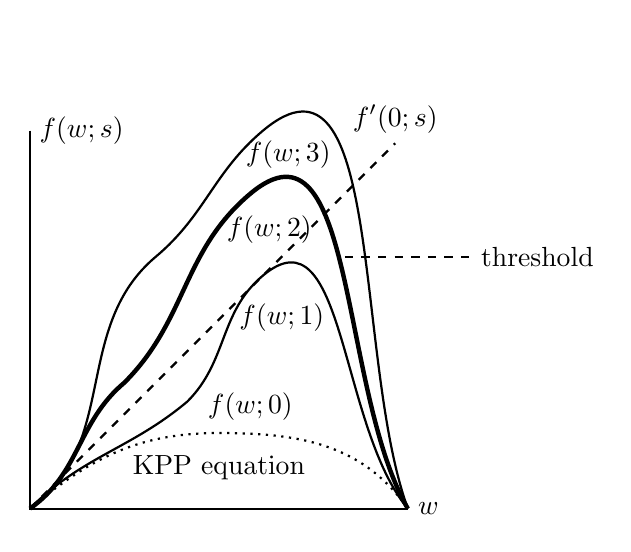
\begin{tikzpicture}[scale = 0.8]
\draw[thick](-3,6)-- (-3,0)-- (3,0) node[right] {$w$};
\draw[dashed] [thick](-3,0)--(2.8,5.8) node[above] {$f'(0;s)$};
\node[right] at (-3,6) {$f(w;s)$};
\draw[dotted] [thick] (-3,0) to [out=40,in=180] (0,1.2) to [out=0,in=125] (3,0);
\node[below] at (0.5,2) {$f(w;0)$};
\node[below] at (0,1) {KPP equation};
%\node[below] at (0,-0.5) {{\bf{Figure 1}}: The transition from linear selection to nonlinear selection};
%\node[below] at (0.5,-1) {of the minimal traveling wave speed of \eqref{Hadeler-Rothe eq}.};
\draw [thick] (-3,0) to [out=45, in=220] (-0.5,1.7) to [out=45,in=220] (0.7,3.7) to [out=40,in=130] (3,0);
\node[below] at (1,3.4) {$f(w;1)$};
\draw [ultra thick] (-3,0) to [out=35, in=220] (-1.5,2) to [out=45,in=220] (0.5,5) to [out=40,in=120] (3,0);
\node[below] at (0.8,4.8) {$f(w;2)$};
\draw [thick] (-3,0) to [out=35, in=220] (-1,4) to [out=40,in=220] (0.7,6) to [out=40,in=110] (3,0);
\node[below] at (1.1,6) {$f(w;3)$};
\draw[dashed] [thick] (2,4)--(4,4) node[right] {threshold};
\end{tikzpicture}
\caption{The transition from linear selection to nonlinear selection of \eqref{Hadeler-Rothe eq}.}
\end{center}
\end{figure}

\subsubsection{The reaction-diffusion equation}

\noindent

We first consider the following single reaction-diffusion equation
\beaa
w_t= w_{xx} +f(w;s),
\eeaa
where
$\{f(\cdot;s)\}\subset C^2$ is a one-parameter family of nonlinear functions satisfying monostable condition and varies continuously and monotonously on the parameter $s\in[0,\infty)$. %That is,
The assumptions on $f$ are as follows:
\begin{itemize}
    \item[(A1)](monostable condition) $f(\cdot;s)\in C^2([0,1])$, $f(0;s)=f(1;s)=0$, $f'(0;s):=\gamma_0>0>f'(1;s)$,  and $f(w;s)>0$ for all $s\in\mathbb{R}^+$ and $w\in(0,1)$.
    \item[(A2)] (Lipschitz continuity) $f(\cdot;s)$, $f'(\cdot;s)$, and $f''(\cdot;s)$ are Lipschitz continuous on $s\in\mathbb{R}^+$
    uniformly in $w$. In other words,
    there exists $L_0>0$ such that
    \beaa
    |f^{(n)}(w;s_1)-f^{(n)}(w;s_2)|\leq L_0|s_1-s_2|\quad \mbox{for all $\ $ $w\in[0,1]$ and $n=0,1,2$,}
    \eeaa
    where $f^{(n)}$ mean the $n$th derivative of $f$ with respect to $w$ for $n\in\mathbb{N}$, i.e. $f^{(0)}=f$, $f^{(1)}=f'$, and $f^{(2)}=f''$.

    \item[(A3)] (monotonicity condition) $f(w;\hat{s})>f(w;s)$ for all $w\in (0,1)$ if $\hat{s}>s$, and $f''(0;\hat{s})> f''(0;s)$ if $\hat{s}>s$.
    %$f(\cdot;s)$ is strictly increasing on $s\in\mathbb{R}^+$,
\end{itemize}


\begin{remark}%\label{rm:A1}
Without loss of generality, we assume $\gamma_0=1$ in (A1), in the part concerned with the single reaction-diffusion equation, such that the linearly selected propagation speed equals to $2$. 
\end{remark}


\begin{remark}
Note that, in this paper, we always assume $\{f(\cdot;s)\}\subset C^2$ as that in (A1) for the simplicity of the proof. As a matter of fact,
our approach still works for weaker regularity of $f$, say
$\{f(\cdot;s)\}\subset C^{1,\alpha}$ for some $\alpha\in(0,1)$.
If we consider a higher degree of regularity for $f$, such as ${f(\cdot;s)}\subset C^k$ for some $k>2$, then the condition in (A3) for $f''(0;\cdot)$ will be replaced by $f^{(i)}(0;\cdot)$ for some $1<i\le k$.
%for $\{f(\cdot;s)\}\subset C^{1,\alpha}$ with weaker regularity, our approach still works.
\end{remark}

%$f'(w;s)$ and $f''(w;s)$ mean the derivative of $f$ with respect to $w$.

Thanks to (A1), there exists the minimal traveling wave speed for all $s\in[0,\infty)$, denoted by $c^*(s)$, such that
the system
\begin{equation}\label{scalar tw-parameter s}
\left\{
\begin{aligned}
&W''+cW'+f(W;s)=0,\quad  \xi\in\mathbb{R},\\
&W(-\infty)=1,\ W(+\infty)=0,\\
&W'<0,\quad \xi\in\mathbb{R},
\end{aligned}
\right.
\end{equation}
admits a unique (up to translations) solution $(c,W)$ if and only if  $c\geq c^*(s)$.

We further assume that linear (resp., nonlinear) selection mechanism can occur at some $s$.
More precisely, $f(\cdot;s)$ satisfies %some additional assumptions as follows:
\begin{itemize}
     %\item[(A1)] $f_s(w)$ is strictly increasing on $s$ for all $s\in\mathbb{R}^+$;
    \item[(A4)] there exists $s_1>0$ such that $f(w;s_1)$ satisfies KPP condition \eqref{kpp condition},
    %if and only if $s\in[0,s_1]$;
   and thus $c^*(s_1)=2$.
    \item[(A5)]  there exists  %$s_1<s_2<\infty$
     $s_2>s_1$ such that $c^*(s_2)>2$.
\end{itemize}

\begin{remark}\label{rk:a4+a5}
In view of (A3), a simple comparison yields that $c^*(\hat{s})\geq c^*(s)$ if $\hat{s}\geq s$.
Together with (A4), (A5) and the fact $c^*(s)\geq 2$ for all $s\geq0$, we see that:
\begin{itemize}
\item[(1)] $c^*(s)=2$ for all $0\leq s\leq s_1$;
\item[(2)] $c^*(s)>2$ for all $s\geq s_2$.
\end{itemize}
\end{remark}


\begin{remark}
It is easy to check that \eqref{Hadeler-Rothe eq} satisfies assumptions  (A1)-(A5).
\end{remark}




Our first main result describes how a pulled front
evolves to a pulled-to-pushed transition front in terms of the varying parameter $s$, which gives a new necessary and sufficient condition to determine linear %selection
and nonlinear selection.
The key point is to completely characterize the evolution of the decay rate of the minimal traveling wave $W_s(\xi)$ with respect to $s$.
It is well known (\cite{Aronson Weinberger}) that if $c^*(s)=2$, then
\bea\label{decay-W-linear}
W_s(\xi)=A\xi e^{-\xi}+Be^{-\xi}+o(e^{-\xi})\quad \mbox{as $\xi\to+\infty$},
\eea
where %$A,B\geq0$ \red{Can B<0 when A>0?}
$A\geq0$ and $B\in \mathbb{R}$,
and $B>0$ if $A=0$. On the other hand, from \cite{Rothe1981}, we see that if $c^*(s)>2$, then
\bea\label{decay-W-nonlinear}
W_s(\xi)=Ae^{-\lambda_s^+\xi}+o(e^{-\lambda_s^+\xi})\quad \mbox{as $\xi\to+\infty$},
\eea
where $A>0$ and
\bea\label{lambda-s}
\lambda^+_{s}:=\frac{c^*(s)+\sqrt{(c^{*}(s))^2-4}}{2}>1.
\eea
As we will see, the key point to understand the speed selection problem is to determine the leading order of the decay rate of $W_s(\xi)$, i.e.
whether $A>0$ or $A=0$ in \eqref{decay-W-linear}.
%we figure out that



\begin{theorem}\label{th: threshold scalar equation}
Assume that (A1)-(A5) hold. Then there exists the threshold value $s^*\in[s_1,s_2)$ such that the minimal traveling wave speed of \eqref{scalar tw-parameter s} satisfies
\begin{equation}\label{def of threshold scalar}
c^*(s)=2\quad\text{for all}\ s\in[0,s^*];\quad c^*(s)>2\quad\text{for all}\ s\in(s^*,\infty).
\end{equation}
Moreover,
the minimal traveling wave $W_s(\xi)$ satisfies %,it holds
\begin{equation}\label{asy tw threshold scalar}
W_s(\xi)=Be^{-\xi}+o(e^{-\xi})\quad \mbox{as}\quad \xi\to+\infty\quad\text{for some}\quad B>0,
\end{equation}
%with $B>0$ as $\xi\to+\infty$
if and only if $s=s^*$.
\end{theorem}


\begin{remark}
\begin{itemize}
\item[(1)]
Note that \eqref{asy tw threshold scalar} in Theorem~\ref{th: threshold scalar equation} indicates that, as $\xi\to+\infty$, the leading order of the decay rate of $W_s(\xi)$ switches from $\xi e^{-\xi}$ to $e^{-\xi}$ as $s\to s^*$ from below.
\item[(2)] In our proof of \eqref{def of threshold scalar} and the sufficient condition for \eqref{asy tw threshold scalar},
the condition in (A3) that $f''(0;\hat{s})> f''(0;s)$ for $\hat{s}>s$ is not required.
\end{itemize}
\end{remark}



Combining \eqref{decay-W-linear}, \eqref{decay-W-nonlinear} and Theorem \ref{th: threshold scalar equation},
we can fully understand how the decay rates of the minimal traveling wave depend on $s$, which is formulated as follows:

%\begin{remark}
\begin{corollary}\label{cor: different minimal tw}
%Let $f(w;s)$ satisfy (A1)-(A5).
Assume that (A1)-(A5) hold. Then asymptotic behaviors of the pulled front, pushed front, and pulled-to-pushed transition front are shown as follows.
\begin{itemize}
    \item[(1)] Pulled front: if $s\in[0,s^*)$, then $W_s(\xi)=A\xi e^{-\xi}+Be^{-\xi}+o(e^{-\xi})$ as $\xi\to+\infty$ with $A>0$ and $B\in \mathbb{R}$;
    \item[(2)] Pulled-to-pushed transition front: if $s=s^*$, then $W_s(\xi)=Be^{-\xi}+o(e^{-\xi})$ as $\xi\to+\infty$ with $B>0$;
    \item[(3)] Pushed front: if $s\in(s^*,\infty)$, then $W_s(\xi)=Ae^{-\lambda_s^+\xi}+o(e^{-\lambda_s^+\xi})$ as $\xi\to+\infty$ with $A>0$.%and
        %\beaa
        %\lambda_{s}:=\frac{c^*(s)+\sqrt{(c^{*}(s))^2-4\beta^2}}{2},
        %\eeaa
\end{itemize}
Here $\lambda_{s}^+$ is defined as \eqref{lambda-s}.
\end{corollary}

\subsubsection{The integro-differential equation}\label{sec: intro nonlocal}

\noindent

Next, we  consider the following single integro-differential equation
\bea\label{nonlocal equation}
w_t= J\ast w-w +f(w;q),
\eea
where
$\{f(\cdot;q)\}\subset C^2$ is a one-parameter family of nonlinear functions satisfying (A1)-(A3) defined in Subsection 1.2.1 with $s=q$, %$q=s$. 
$J$ is a nonnegative dispersal kernel defined on $\mathbb{R}$, and $J\ast w$ is defined as
$$J\ast w(x):=\int_{\mathbb{R}}J(x-y)w(y)dy.$$ %That is,
For the simplicity of our discussion, throughout this paper, we always assume that the dispersal kernel
\begin{equation}\label{assumption on J}
J\ \text{is compactly supported, symmetric, and}\ \int_{\mathbb{R}}J=1.
\end{equation}



%$f'(w;s)$ and $f''(w;s)$ mean the derivative of $f$ with respect to $w$.

Under the assumption (A1), it has been proved in \cite{Coville} that there exists the minimal traveling wave speed for all $q\in[0,\infty)$, denoted by $c_{NL}^*(q)$, such that
the system
\begin{equation}\label{scalar nonlocal tw-parameter s}
\left\{
\begin{aligned}
&J\ast \mathcal{W}+c\mathcal{W}'+f(\mathcal{W};q)-\mathcal{W}=0,\quad  \xi\in\mathbb{R},\\
&\mathcal{W}(-\infty)=1,\ \mathcal{W}(+\infty)=0,\\
&\mathcal{W}'<0,\quad \xi\in\mathbb{R},
\end{aligned}
\right.
\end{equation}
admits a unique (up to translations) solution $(c,\mathcal{W})$ if and only if
$c\geq c_{NL}^*(q)$. %\ge c_0^*$.
Moreover, there is a lower bound estimate for the minimal speed $c_{NL}^*(q)\geq c_0^*$,
where the critical speed $c_0^*$ is given by the following variational formula
\begin{equation}\label{formula of c_NL}
c_{0}^*:=\min_{\lambda>0}\frac{1}{\lambda}\Big(\int_{\mathbb{R}}J(x)e^{\lambda x}dx+f'(0;q)-1\Big),
\end{equation}
which derived from the linearization of \eqref{scalar nonlocal tw-parameter s} at the trivial state $\mathcal{W}= 0$.
If $f(\cdot;q)$ also satisfies the KPP condition \eqref{kpp condition}, then
$c_{NL}^*(q)= c_0^*$. Therefore, we call the case $c_{NL}^*(q)= c_0^*$ as the speed linear selection and the case $c_{NL}^*(q)> c_0^*$ as the speed nonlinear selection.



\begin{remark}\label{rm:lambda_0}
Let $h(\lambda)$ be defined by
$$h(\lambda):=\int_{\mathbb{R}}J(z)e^{\lambda z}dz-1+f'(0;q).$$
It is easy to check that $\lambda\to h(\lambda)$ is an increasing, strictly convex, and sublinear function satisfying $h(0)=f'(0;q)>0$.
Therefore, there exist only one $\lambda_0>0$ satisfying $h(\lambda_0)=c_0^*\lambda_0$, and for $c>c_0^*$, the equation $h(\lambda)=c\lambda$ admits two different positive roots $\lambda_q^-(c)$ and $\lambda_q^+(c)$ satisfying $0<\lambda_q^-(c)<\lambda_0<\lambda_q^+(c)$. Since only the minimal traveling wave is considered in this paper, we denote $\lambda_q^{\pm}(c):=\lambda_q^{\pm}$ for simplicity.
\end{remark}



We further assume that a linear (resp., nonlinear) selection mechanism can occur at some $q$.
More precisely, $f(\cdot;q)$ satisfies %some additional assumptions as follows:
\begin{itemize}
     %\item[(A1)] $f_s(w)$ is strictly increasing on $s$ for all $s\in\mathbb{R}^+$;
    \item[(A6)] there exists $q_1>0$ such that $f(w;q_1)$ satisfies KPP condition \eqref{kpp condition},
    %if and only if $s\in[0,s_1]$;
   and thus $c_{NL}^*(q_1)=c^*_0$.
    \item[(A7)]  there exists  %$s_1<s_2<\infty$
     $q_2>q_1$ such that $c_{NL}^*(q_2)>c^*_0$.
\end{itemize}

\begin{remark}\label{rk:a6+a7}
In view of (A3), a simple comparison yields that $c_{NL}^*(\hat{q})\geq c_{NL}^*(q)$ if $\hat{q}\geq q$.
Together with (A6), (A7) and the fact 
$c_{NL}^*(q)\geq c^*_0\ \ \text{for all}\ \ q\geq0,$
we see that
$$c_{NL}^*(q)=c^*_0\ \ \text{for all}\ \ 0\leq q\leq q_1\ \ \text{and}\ \ c_{NL}^*(q)>c^*_0\ \ \text{for all}\ \ q\geq q_2.$$
\end{remark}


It has been proved in \cite{Carr Chmaj} by Ikehara's Theorem that, if $f(w;q)$ satisfies the KPP condition \eqref{kpp condition}, then
\beaa
\mathcal{W}_q(\xi)=A\xi e^{-\lambda_0\xi}+Be^{-\lambda_0\xi}+o(e^{-\lambda_0\xi})\quad \mbox{as $\xi\to+\infty$},
\eeaa
where $A>0$ and $B\in \mathbb{R}$.
The asymptotic estimate %has been
can be extended to the general monostable case (i.e.(A1)) %by \cite{Coville}
as follows:
\begin{itemize}
\item[(1)] if $c_{NL}^*(q)=c^*_0$ and $c=c_{NL}^*(q)$, then
\bea\label{decay-U-linear-1}
\mathcal{W}_q(\xi)=A\xi e^{-\lambda_0\xi}+Be^{-\lambda_0\xi}+o(e^{-\lambda_0\xi})\quad \mbox{as $\xi\to+\infty$},
\eea
where $A\geq0$ and $B\in \mathbb{R}$,
and $B>0$ if $A=0$.
\item[(2)] if $c_{NL}^*(q)\ge c^*_0$ and $c>c_{NL}^*(q)$, then
\bea\label{decay-U-nonlinear}
\mathcal{W}_q(\xi)=Ae^{-\lambda^-_q\xi}+o(e^{-\lambda_q^-\xi})\quad \mbox{as $\xi\to+\infty$},
\eea
where $A>0$ and $\lambda^-_q$ is defined in Remark \ref{rm:lambda_0}.
\end{itemize}
We remark that \eqref{decay-U-linear-1} and \eqref{decay-U-nonlinear} has been discussed in
\cite{Coville}; however, the proof provided in \cite[Theorem 1.6]{Coville} contains a gap such that they deduced that $A>0$ always holds in \eqref{decay-U-linear-1}.
We will fix the gap in Proposition~\ref{prop:correction-U-linear-decay} below.


The first result is concerned with how the {\em pulled front} %change
evolves to the pulled-to-pushed transition front in terms of the varying parameter $q$. Similar to Theorem \ref{th: threshold scalar equation}, the key point is to completely characterize the evolution of the decay rate of the minimal traveling wave $\mathcal{W}_q(\xi)$ with respect to $q$.

\begin{theorem}\label{th: threshold scalar equation nonlocal}
Assume that (A1)-(A3) and (A6)-(A7) hold. Then there exists the threshold value $q^*\in[q_1,q_2)$ such that the minimal traveling wave speed of \eqref{scalar nonlocal tw-parameter s} satisfies
\begin{equation}\label{def of threshold scalar nonlocal}
c_{NL}^*(q)=c_0^*\quad\text{for all}\ q\in[0,q^*];\quad c_{NL}^*(q)>c_0^*\quad\text{for all}\ q\in(q^*,\infty).
\end{equation}
Moreover,
the minimal traveling wave $U_s(\xi)$ satisfies %,it holds
\begin{equation}\label{asy tw threshold scalar nonlocal}
\mathcal{W}_q(\xi)=Be^{-\lambda_0\xi}+o(e^{-\lambda_0\xi})\quad \mbox{as}\quad \xi\to+\infty\quad\text{for some}\quad B>0,
\end{equation}
 %with $B>0$ as $\xi\to+\infty$
if and only if $q=q^*$.
\end{theorem}


\begin{remark}
Note that, \eqref{asy tw threshold scalar nonlocal} in Theorem~\ref{th: threshold scalar equation nonlocal} indicates that, as $\xi\to+\infty$, the leading order of the decay rate of $\mathcal{W}_q(\xi)$ switches from $\xi e^{-\lambda_0\xi}$ to $e^{-\lambda_0\xi}$ as $q\to q^*$ from below.
\end{remark}

\begin{remark}
In our proof of \eqref{def of threshold scalar nonlocal} and the sufficient condition for \eqref{asy tw threshold scalar nonlocal},
the condition in (A3) that $f''(0;\hat{q})> f''(0;q)$ for $\hat{q}>q$ is not required.
\end{remark}

Our second result is concerned with the asymptotic behavior of the minimal traveling wave in the case when
$c_{NL}^*(q)>c^*_0$. In the reaction-diffusion case, it decays with a fast rate (see the statement (3) of Corollary \ref{cor: different minimal tw}). In this paper, we will prove that the conclusion holds true also for the integro-differential case. Furthermore, with \eqref{decay-U-linear} and Theorem \ref{th: threshold scalar equation nonlocal},
we can fully understand how the decay rates of the minimal traveling wave depend on $q$, which is formulated as follows:
\begin{corollary}\label{cor: different minimal tw nonlocal}
%Let $f(w;s)$ satisfy (A1)-(A5).
Assume that (A1)-(A3) and (A6)-(A7) hold. Then asymptotic behaviors of the pulled front, pushed front, and pulled-to-pushed transition front are shown as follows.
\begin{itemize}
    \item[(1)] Pulled front: if $q\in[0,q^*)$, then $\mathcal{W}_q(\xi)=A\xi e^{-\lambda_0\xi}+Be^{-\lambda_0\xi}+o(e^{-\lambda_0\xi})$ as $\xi\to+\infty$ with $A>0$ and $B\in \mathbb{R}$;
    \item[(2)] Pulled-to-pushed transition front: if $q=q^*$, then $\mathcal{W}_q(\xi)=Be^{-\lambda_0\xi}+o(e^{-\lambda_0\xi})$ as $\xi\to+\infty$ with $B>0$;
    \item[(3)] Pushed front: if $q\in(q^*,\infty)$, then $\mathcal{W}_q(\xi)=Ae^{-\lambda^+_q\xi}+o(e^{-\lambda^+_q\xi})$ as $\xi\to+\infty$ with $A>0$.%and
\end{itemize}
Here $\lambda^+_{q}$ is defined as that in Remark \ref{rm:lambda_0}.
\end{corollary}

\begin{remark}\label{rm: asy of minimal tw nonlinear case}
The asymptotic behaviors of the pushed front is crucial for understanding the long-time behavior of the solution of the Cauchy problem (see \cite{Rothe1981} for the scalar reaction-diffusion equation and \cite{Wu Xiao Zhou} for the Lotka-Volterra competition-diffusion system). 
\end{remark}

\begin{remark}\label{rm: solved an open}
We remark that (3) of Corollary~\ref{cor: different minimal tw nonlocal} indicates that the pushed front always has a fast decay, which answers an open problem given in \cite{Bonnefon Coville Garnier Roques2014}. 
%As one of the applications of our main methodology, we will show that the pushed front always has a fast decay, particularly for integro-differential equations. 
More importantly, our approach is applicable to establish the decay rate of pushed fronts for more general monostable equations and systems as long as the comparison principle holds.
\end{remark}


\subsection{Outline of the paper}
The rest of this paper is organized as follows. 

In Section 2, we study the speed selection mechanism
for the single reaction-diffusion equation, where Theorem \ref{th: threshold scalar equation} is established. The construction of a super-solution to prove the sufficient condition is the most involved part, while the necessary condition is proved by applying the sliding method.

Sections 3, 4, and 5 are devoted to the speed selection problem for the Lotka-Volterra competition system.
In Section 3, we propose a sufficient condition, established by the singular perturbation method,  under which the propagation speed of the Lotka-Volterra competition system is nonlinearly selected.
This condition highlights the importance of expanding the common parameter range 
$0<a<1<b$ to $0<a<1,\ b>0$. 
In Section 4, we extend our argument to the Lotka-Volterra competition system and complete the proof of Theorem \ref{th:threshold}. 

In Section 5, we address the continuity of spreading speed on parameters $a>0,\ b>1$, including the degenerate case $a=1$. %either $a=1$ or $b=1$
By establishing the existence of the minimal traveling wave speed and its sign in the case where $a=1$ and $b>1$, %by studying the sign of the traveling wave speed for the case $a=1$ and $b>1$
we establish another sufficient condition for speed nonlinear selection and discover a new criterion for determining the sign of the wave speed for bistable fronts.

In Section 6, we extend our analysis to integro-differential equations and complete the proof of Theorem \ref{th: threshold scalar equation nonlocal}. 
The challenge in this extension is accurately on how to characterize the propagation fronts.

In Section 7, we make a conclusion of our observations regarding the speed selection problem and provide a complete classification of the minimal traveling wave fronts, i.e. Corollary \ref{cor: different minimal tw system},  \ref{cor: different minimal tw}, and \ref{cor: different minimal tw nonlocal}.

In the end of this paper,
the Appendix section is devoted to the results for the existence of the minimal traveling wave speed
of \eqref{tw solution weak}, the asymptotic behavior of traveling waves of \eqref{tw solution weak} under condition ({\bf H}), and the asymptotic behavior of traveling waves of intergo-differential equation \eqref{scalar nonlocal tw-parameter s}.  It also includes
proofs for results that have not been previously established in the literature.

%The rest of this paper is organized as follows. In Section~\ref{sec:threshold-system}, we study
%the speed selection mechanism for a two-species competition system, where Theorem~\ref{th:threshold} is established.
%In the end of this paper, the Appendix section is devoted to the results for the existence of the minimal traveling wave speed of \eqref{system} and the asymptotic behavior of traveling wave at $\pm\infty$ under condition {\bf(H)}. It also includes proofs for results that have not been previously established in the literature.}

\section{Threshold of the reaction-diffusion equation}\label{sec:threshold scalar}


In this section, we aim to prove Theorem~\ref{th: threshold scalar equation}.
First, it is well known that for each $s\geq0$, under (A1), the minimal traveling wave is unique (up to a translation).
Together with (A2), one can use the standard compactness argument to conclude that $c^*(s)$ is continuous for all $s\ge 0$.
It follows from (A3)-(A5) and Remark~\ref{rk:a4+a5} that $c^*(s)$ is nondecreasing in $s$. Thus, we immediately obtain the following result.

\begin{lemma}\label{lem: th1-part1}
Assume that (A1)-(A5) hold. Then there exists a threshold $s^*\in[s_1,s_2)$ such that \eqref{def of threshold scalar} holds.
\end{lemma}



Thanks to Lemma~\ref{lem: th1-part1}, to prove Theorem~\ref{th: threshold scalar equation}, it suffices to show that
\eqref{asy tw threshold scalar} holds if and only if $s=s^*$.
Let $W_{s^*}$ be the minimal traveling wave satisfying \eqref{scalar tw-parameter s} with $s=s^*$
and $c^*(s^*)=2$. For simplicity, we denote $W_*:=W_{s^*}$.
The first and the most involved step is to show that if $s=s^*$, then \eqref{asy tw threshold scalar} holds.
%the second statement of Theorem \ref{th: threshold scalar equation}.
To do this, we shall use a contradiction argument.
Assume that \eqref{asy tw threshold scalar} is not true. Then, %by Lemma~\ref{lm: behavior around + infty}, we can find $A_0>0$ such that
it holds that (cf. \cite{Aronson Weinberger})
\bea\label{AS-U-infty-for-contradiction scalar}
\lim_{\xi\rightarrow+\infty}\frac{W_{*}(\xi)}{\xi e^{-\xi}}=A_0\quad \mbox{for some $A_0>0$.}
\eea

%Since $c^*(b^*)=2\sqrt{1-a}$ (Lemma~\ref{lm: existence b*}), we see that $\lambda_u>\lambda_v$ is equivalent to
%\beaa
%\frac{-2\sqrt{1-a}}{2}>\frac{-2\sqrt{1-a}-\sqrt{(2\sqrt{1-a}\,)^2+4rd}}{2d},
%\eeaa
%which implies that
%\begin{equation}\label{condition lambda_u>lambda_v}
%(d-2)(1-a)<r.
%\end{equation}
%Also, by Lemma~\ref{lm: behavior around + infty}, we have
%\bea\label{AS-V-infty-for-contradiction}
%\lim_{\xi\rightarrow+\infty}\frac{1-V_{*}(\xi)}{\xi^{} e^{\lambda_u\xi}}=C_0
%\eea
%for some $C_0>0$.


Under the condition \eqref{AS-U-infty-for-contradiction scalar},
we shall prove the following proposition.

\begin{proposition}\label{Prop-supersol}
Assume that (A1)-(A5) hold. In addition, if \eqref{AS-U-infty-for-contradiction scalar} holds,
then there exists an auxiliary continuous function $R_w(\xi)$ defined in $\mathbb{R}$ satisfying
\begin{equation}\label{decay rate of Rw}
R_w(\xi)=O(\xi e^{-\xi}) \quad \mbox{as $\xi\to\infty$},
\end{equation}
such that 
$$\bar{W}(\xi):=\min\{W_{*}(\xi)-R_w(\xi),1\}\geq (\not\equiv) 0$$
is a super-solution
satisfying
\bea\label{tw super solution scalar}
&N_0[\bar W]:=\bar W''+2\bar W'+f(\bar W;s^*+\delta_0)\le0,\quad  \mbox{a.e. in $\mathbb{R}$},
\eea
%forms a super-solution  of \eqref{scalar tw-parameter s} with $s=s^*$.
%\begin{equation}\label{tw super solution scalar}
%\left\{
%\begin{aligned}
%&N_0[\bar W]:=\bar W''+2\beta\bar W'+f(\bar W;s^*+\delta_0)\le0,\quad  \mbox{a.e. in $\mathbb{R}$,}\\
%&\bar W(-\infty)=1,\ \bar W(+\infty)=0,\\
%&0\leq \bar W(\xi) \leq 1, \quad  \mbox{in $\mathbb{R}$,}\\
%&\bar W'(\xi)\leq 0,\quad   \mbox{a.e. in $\mathbb{R}$,}
%\end{aligned}
%\right.
%\end{equation}
for some small $\delta_0>0$,
%for all sufficiently small $\delta_0>0$, 
where ${\bar W}'(\xi_0^{\pm})$ exists and
${\bar W}'(\xi_0^+)\leq {\bar W}'(\xi_0^-)$
if $\bar W'$ is not continuous at $\xi_0$.

\end{proposition}
%\blue{In general, we may call such $\bar W$ a {\em super-solution} of $N_0[W]=0$.}
%It is easy to see that such a $\bar{W}(\xi):=(W_{s^*}-R_w)(\xi)$ forms a super-solution  of \eqref{scalar tw-parameter s} with $s=s^*$.

Next, we shall go through a lengthy process to prove Proposition~\ref{Prop-supersol}.
Hereafter, (A1)-(A5) are always assumed.

%we now show that, for any sufficiently small $\sigma>0$, there exists an auxiliary function $R_w(\xi)$  with
%\begin{equation}\label{decay rate of Rw}
%R_w(\xi)=O(\xi e^{-\beta\xi}) \quad \mbox{as $\xi\to\infty$},
%\end{equation}
%such that $\bar{W}(\xi):=(W_*-R_w)(\xi)$ forms a super-solution satisfying
%\begin{equation}\label{tw super solution scalar}
%\left\{
%\begin{aligned}
%&N_0[\bar W]:=\bar W''+(2\beta+\sigma)\bar W'+f(\bar W;s^*+\delta_0)\le0,\\
%&\bar W(-\infty)=1,\ \bar W(+\infty)=0,\ \bar W'< 0,
%\end{aligned}
%\right.
%\end{equation}
%for \red{some small $\sigma>0$} and some sufficiently small $\delta_0>0$ which is independent of $\sigma$.

%%In order to state of our argument,
%\red{The construction of $R_w$ depends on the sign of $f''(0;s^*)0$; so
%we divide %the shapes of $f(w;s^*)$ around $0$
%our discussion into three cases: %(1) $f''(0;s^*)>0$; (2) $f''(0;s^*)<0$; (3) $f''(0;s^*)=0$.
%\bea
%\mbox{Case 1: $f''(0;s^*)>0$\quad  Case 2: $f''(0;s^*)>0$\quad  Case 3: $f''(0;s^*)=0$.}
%\eea
%}


From (A1), by shifting the coordinates, we can immediately obtain
the following lemma.
%%a lemma as follows.

\begin{lemma}\label{lm: divide R to 3 parts}
%%Let $M>0$ be an arbitrarily large constant and
Let $\nu_{1}>0$ be %some
an arbitrary constant. Then there exist
$$-\infty<\xi_2<0<\xi_1<+\infty\ \ \text{with}\ \ |\xi_1|,|\xi_2|\ \text{very large},$$
such that
the following hold:
\begin{itemize}
    \item[(1)]
    $\dps f(W_{*}(\xi);s^*)=W_{*}(\xi)+\frac{f''(0;s^*)}{2}W^2_{*}(\xi)+o(W^2_{*}(\xi))$ for all $\xi\in[\xi_1,\infty)$;
    \item[(2)]  $f'(W_{*}(\xi);s^*)<0$ for all $\xi\in(-\infty,\xi_2]$.
\end{itemize}
\end{lemma}


\subsection{Construction of the super-solution}\label{subsec-2-1}

\noindent

Let us define $R_w(\xi)$ as (see Figure \ref{Figure scalar})
\begin{equation}\label{definition of Rw}
R_w(\xi)=\begin{cases}
\varepsilon_1\sigma(\xi) e^{-\xi},&\ \ \mbox{for}\ \ \xi\ge\xi_{1}+\delta_1,\\
\varepsilon_2 e^{\lambda_1\xi},&\ \ \mbox{for}\ \ \xi_{2}+\delta_2\le\xi\le\xi_{1}+\delta_1,\\
\varepsilon_3\sin(\delta_4(\xi-\xi_2)),&\ \ \mbox{for}\ \ \xi_2-\delta_3\le\xi\le\xi_2+\delta_2,\\
-\varepsilon_4e^{\lambda_2\xi},&\ \ \mbox{for}\ \ \xi\le\xi_2-\delta_3,
\end{cases}
\end{equation}
where $\delta_{i=1,\cdots,4}>0$, $\lambda_{n=1,2}>0$, and $\sigma(\xi)>0$ will be
determined such that $\bar W(\xi)$ satisfies \eqref{decay rate of Rw} and \eqref{tw super solution scalar}. Moreover, we should choose
positive $\varepsilon_{j=1,\cdots,4}\ll A_0$ ($A_0$ is defined in \eqref{AS-U-infty-for-contradiction scalar}) such that $R_w(\xi)\ll W_*(\xi)$ and $\bar W(\xi)$ is continuous for all $\xi\in\mathbb{R}$.


Since $f(\cdot;s^*)\in C^2$, there exist $K_1>0$ and $K_2>0$ such that
\bea\label{K1K2}
|f''(W_*(\xi);s^*)|< K_1,\quad |f'(W_*(\xi);s^*)|< K_2\quad \mbox{for all}\quad\xi\in\mathbb{R}.
\eea
%$|f''(W_*(\xi);s^*)|< K_1$ and
%$|f'(W_*(\xi);s^*)|< K_2$ for all $\xi\in\mathbb{R}$.
We set $\lambda_1>0$ %($L_0$ is defined in (A2))
large enough such that
\begin{equation}\label{condition on lambda 1}
-2\lambda_1-\lambda_1^2+K_2<0\ \text{and}\ \lambda_1>K_2.
\end{equation}
Furthermore, there exists $K_3>0$ such that
\begin{equation}\label{condition on xi_2 scalar}
f'(W_*(\xi); s^*)\le -K_3<0\quad\text{for all}\quad\xi\le \xi_2.
\end{equation}
We set 
$$0<\lambda_2<\lambda_w:=\sqrt{1-f'(1;s^*)}-1$$
sufficiently small
such that
\bea\label{lambda 2}
\lambda_2^2+2\lambda_2-K_3<0.
\eea

%Since $W_*(+\infty)=0$ and $W_*(-\infty)=1$, for any given small $\rho>0$, there exists $M>0$ large enough
%such that
%\begin{equation}\label{rho}
%\begin{cases}
%0< W_*(\xi)<\rho\quad\text{for all}\quad\xi\geq M\\
%1-\rho<W_*(\xi)<1\quad\text{for all}\quad\xi\geq -M.
%\end{cases}
%\end{equation}
%Moreover, up to enlarging $\xi_1$, we may assume $\xi_1>M$.



\begin{figure}
\begin{center}
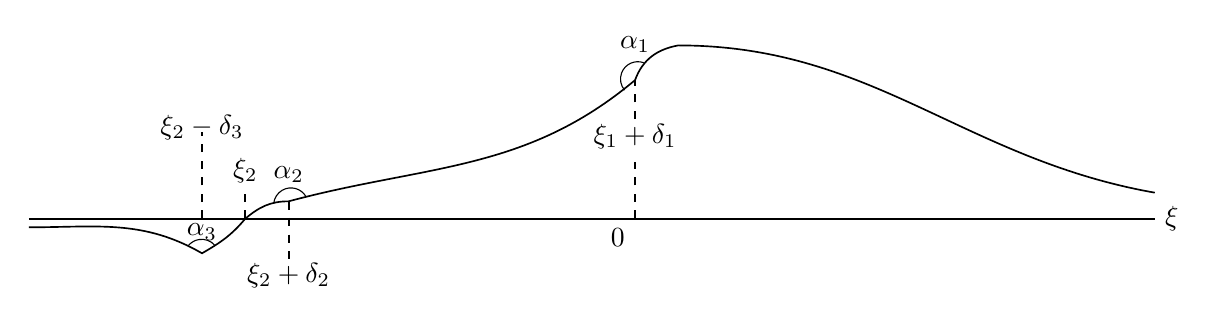
\begin{tikzpicture}[scale = 1.1]
\draw[thick](-6,0) -- (7,0) node[right] {$\xi$};
\draw [semithick] (-6, -0.1) to [ out=0, in=150] (-4,-0.4) to [out=30, in=230] (-3.5,0)  to [out= 40, in=180] (-3,0.2) to [out=15, in=220] (1,1.6) to [out=70,in=190] (1.5,2) to [out=0,in=170] (7,0.3);
\node[below] at (1,1.2) {$\xi_{1}+\delta_1$};
\node[below] at (0.8,0) {$0$};
\draw[dashed] [thick] (-3.5,0)-- (-3.5,0.3);
\node[above] at (-3.5,0.3) {$\xi_2$};
\draw[dashed] [thick] (-3,0.2)-- (-3,-0.5);
\draw[dashed] [thick] (-4,0)-- (-4,1);
\node[above] at (-4,0.8) {$\xi_2-\delta_3$};
\draw[dashed] [thick] (1,0)-- (1,0.65);
\draw[dashed] [thick] (1,1.15)-- (1,1.6);
\node[below] at (-3,-0.4) {$\xi_2+\delta_2$};
\draw [thin] (-3.85,-0.31) arc [radius=0.2, start angle=40, end angle= 140];
\node[above] at (-4,-0.36) {$\alpha_3$};
%\draw [thin] (-2.3,0.355) arc [radius=0.2, start angle=30, end angle= 175];
%\node[above] at (-2.5,0.35) {$\alpha_4$};
\draw [thin] (-2.8,0.255) arc [radius=0.2, start angle=30, end angle= 175];
\node[above] at (-3,0.3) {$\alpha_2$};
\draw [thin] (1.1,1.8) arc [radius=0.2, start angle=70, end angle= 220];
\node[above] at (1,1.8) {$\alpha_1$};
%\node[above] at (2.5,0.5) {\Large{$R_w$}};
%\node[below] at (1,-1.3) {Figure \ref{Figure scalar}: the construction of $R_w(\xi)$.};
\end{tikzpicture}
\caption{the construction of $R_w(\xi)$.}\label{Figure scalar}
\end{center}
\end{figure}


%Next, we will show that there exist positive $\mu_{n=1,2,3}$, $\delta_{i=0,\cdots,6}$, $\varepsilon_{j=1,\cdots,6}$ and %$\eta_{k=1,\cdots,6}$ such that
%$(W_u,W_v)$ satisfies \eqref{tw super solution case 2}.

\medskip





We now divide the proof into several steps.

\noindent{\bf{Step 1}:} We consider $\xi\in[\xi_1+\delta_1,\infty)$ where $\delta_1>0$ is small enough and will be determined in Step 2.
In this case, we have
\beaa
R_w(\xi)=\varepsilon_1\sigma(\xi)\ e^{-\xi}
\eeaa
for some small $\varepsilon_1\ll A_0$ 
such that $\bar W=W_*-R_w>0$ for $\xi\geq \xi_1+\delta_1$.



Note that $W_*$ satisfies \eqref{scalar tw-parameter s} with $c=2$.
By some  straightforward computations, we have
\begin{equation}\label{N0 inequality step 1}
\begin{aligned}
N_0[\bar W]=&-R''_w-2 R'_w-f(W_*;s^*)+f(W_*-R_w;s^*+\delta_0)\\
=&-R''_w-2 R'_w-f(W_*;s^*)+f(W_*-R_w;s^*)\\
&-f(W_*-R_w;s^*)+f(W_*-R_w;s^*+\delta_0).
\end{aligned}
\end{equation}
By the assumption (A1) and the statement (1) of Lemma \ref{lm: divide R to 3 parts}, since $W_*\ll 1$ and $R_w\ll W_*$ for $\xi\in[\xi_1+\delta_1,\infty)$, we have
\begin{equation}\label{estimate 1}
-f(W_*;s^*)+f(W_*-R_w;s^*)= -R_w+f''(0;s^*)(\frac{R^2_w}{2}-W_*R_w)+o((W_*)^2).
\end{equation}
By the assumption (A2) and the statement (1) of Lemma \ref{lm: divide R to 3 parts}, there exists $C_1>0$ such that
\begin{equation}\label{estimate 2}
-f(W_*-R_w;s^*)+f(W_*-R_w;s^*+\delta_0)\le C_1\delta_0(W_*-R_w)^2+o((W_*)^2).
\end{equation}
From \eqref{K1K2}, \eqref{N0 inequality step 1}, \eqref{estimate 1}, \eqref{estimate 2}, % and Lemma \ref{lm: divide R to 3 parts}, 
we have
\bea\label{estimate 3}
N_0[\bar W]\le -\varepsilon_1\sigma''e^{-\xi}+K_1(\frac{R_w^2}{2}+W_*R_w)+C_1\delta_0W_*^2+o((W_*)^2.
\eea


Now, we define
$$\sigma(\xi):=4e^{-\frac{1}{2}(\xi-\xi_1)}-4+4\xi-4\xi_1$$
which satisfies 
$$\sigma(\xi_1)=0,\ \sigma'(\xi)=4-2e^{-\frac{1}{2}(\xi-\xi_1)},\ \sigma''(\xi)=e^{-\frac{1}{2}(\xi-\xi_1)}.$$
Moreover, $\sigma(\xi)= O(\xi)$ as $\xi\to\infty$ implies that $R_w$ satisfies \eqref{decay rate of Rw}.

Due to \eqref{AS-U-infty-for-contradiction scalar} and the equation of $W_*$, we may also assume
\bea\label{W-M}
W_*(\xi) \leq 2A_0\xi e^{-\xi}\quad \mbox{for all}\quad\xi\geq \xi_1.
\eea
Then, from \eqref{estimate 3}, up to enlarging $\xi_1$ if necessary, we always have %can find a small $\delta_0>0$ such that
\beaa
N_0[\bar W]\le -\varepsilon_1e^{-\frac{1}{2}(\xi-\xi_1)}e^{-\xi}+K_1(\frac{R_w^2}{2}+W_*R_w)+C_1\delta_0W_*^2+o((W_*)^2)\le 0
\eeaa
for all sufficiently small $\delta_0>0$
since $R_w^2(\xi)$, $W_*R_w(\xi)$, and  $W_*^2(\xi)$ are $o(e^{-\frac{3}{2}\xi})$
%for $\xi\ge \xi_1$ 
as $\xi\to\infty$
from \eqref{W-M} and the definition of $R_w$.
Therefore, $N_0[\bar W]\leq 0$ for $\xi\ge \xi_1$.


\medskip


\noindent{\bf{Step 2:}} We consider $\xi\in[\xi_2+\delta_2,\xi_1+\delta_1]$ for some small $\delta_2>0$, and small $\delta_1>0$ satisfying
\bea\label{cond delta 1 scalar}
1+3(1-e^{-\frac{\delta_1}{2}})-2\delta_1>0.
\eea
From the definition of $R_w$ in Step 1, it is easy to check that $R'_w((\xi_1+\delta_1)^+)>0$ under the condition \eqref{cond delta 1 scalar}.
In this case, we have $R_w(\xi)=\varepsilon_2 e^{\lambda_1\xi}$
for some large $\lambda_1>0$ satisfying \eqref{condition on lambda 1}.

We first choose
\begin{equation}\label{condition on epsilon 2-RD}
\varepsilon_2=\varepsilon_1\Big(4e^{-\frac{\delta_1}{2}}-4+4\delta_1\Big)e^{-(1+\lambda_1)(\xi_1+\delta_1)}
\end{equation}
such that $R_w(\xi)$ is continuous at $\xi=\xi_{1}+\delta_1$. Then, from \eqref{condition on epsilon 2-RD}, we have
$$R'_w((\xi_1+\delta_1)^{+})=\varepsilon_1\sigma'(\xi_1+\delta_1)e^{-(\xi_1+\delta_1)}- R_w(\xi_1+\delta_1)>R'_w((\xi_1+\delta_1)^{-})=\lambda_1R_w(\xi_1+\delta_1)$$
is equivalent to
$$1+(3+2\lambda_1)(1-e^{-\frac{\delta_1}{2}})>2(1+\lambda_1)\delta_1,$$
which holds by taking $\delta_1$ sufficiently small.
This implies that $\angle\alpha_1<180^{\circ}$.

By some  straightforward computations, we have
\begin{equation*}
\begin{aligned}
N_0[\bar W]=&-(2\lambda_1+\lambda_1^2)R_w-f(W_*;s^*)+f(W_*-R_w;s^*+\delta_0)\\
=&-(2\lambda_1+\lambda_1^2)R_w-f(W_*;s^*)+f(W_*-R_w;s^*)\\
&-f(W_*-R_w;s^*)+f(W_*-R_w;s^*+\delta_0).
\end{aligned}
\end{equation*}
%For $\xi\in[\xi_2+\delta_2,\xi_1+\delta_1]$,
Thanks to \eqref{K1K2}, we have
$$-f(W_*;s^*)+f(W_*-R_w;s^*)< K_2R_w.$$
Moreover, by assumption (A2), %there exists $C_2>0$ such that
$$-f(W_*-R_w;s^*)+f(W_*-R_w;s^*+\delta_0)\le L_0\delta_0.$$
Then, %by setting
since
$\lambda_1$ satisfies \eqref{condition on lambda 1}, we have
$$L_0\delta_0<\varepsilon_2(\lambda_1^2+2\lambda_1-K_2) e^{\lambda_1(\xi_2+\delta_2)}$$
for all sufficiently small $\delta_0>0$,
which implies that $N_0[\bar W]\le 0$ for all $\xi\in[\xi_2+\delta_2,\xi_1+\delta_1]$.


\medskip





\noindent{\bf{Step 3:}} We consider $\xi\in[\xi_2-\delta_3,\xi_2+\delta_2]$ for some small $\delta_2,\delta_3>0$. In this case, $R_w(\xi)=\varepsilon_3\sin(\delta_4(\xi-\xi_2))$.
We first verify the following Claim.
\begin{claim}\label{cl scalar}
For any $\delta_2$ with $\delta_2>\frac{1}{\lambda_1}$, there exist
$\varepsilon_3>0$ and small $\delta_4>0$
such that 
$$R_w((\xi_2+\delta_2)^+)=R_w((\xi_2+\delta_2)^-)$$ 
and $\angle\alpha_2<180^{\circ}$.
\end{claim}
\begin{proof}
Note that 
$$R_w((\xi_2+\delta_2)^+)=\varepsilon_2e^{\lambda_1(\xi_2+\delta_2)},\ R_w((\xi_2+\delta_2)^-)=\varepsilon_3\sin(\delta_4\delta_2).$$
Therefore, we may take
\bea\label{epsilon 3}
\varepsilon_3= \frac{\varepsilon_2e^{\lambda_1(\xi_2+\delta_2)}}{\sin(\delta_4\delta_2)}>0
\eea
such that $R_w((\xi_2+\delta_2)^+)=R_w((\xi_2+\delta_2)^-)$.

By some  straightforward computations, we have
$R'_w((\xi_2+\delta_2)^+)=\lambda_1\varepsilon_2e^{\lambda_1(\xi_2+\delta_2)}$ and
\beaa
R'_w((\xi_2+\delta_2)^-)=\varepsilon_3\delta_4\cos(\delta_4\delta_2)=\frac{\varepsilon_2e^{\lambda_1(\xi_2+\delta_2)}}{\sin(\delta_4\delta_2)}\delta_4\cos(\delta_4\delta_2),
\eeaa
which yields that
$$R'_w((\xi_2+\delta_2)^-)\rightarrow \varepsilon_2e^{\lambda_1(\xi_2+\delta_2)}/\delta_2\ \ \text{as}\ \ \delta_4\to0.$$
In other words, as $\delta_4\to0$,
\bea\label{delta 2}
R'_w((\xi_2+\delta_2)^+)>R'_w((\xi_2+\delta_2)^-)\ \ \text{is equivalent to}\ \ \delta_2>\frac{1}{\lambda_1}.
\eea
Therefore, we can choose $\delta_4>0$ sufficiently small so that $\angle\alpha_2<180^{\circ}$.
This completes the proof of Claim~\ref{cl scalar}.
\end{proof}

Next, we verify the differential inequality of $N_0[\bar W]$ for $\xi\in[\xi_2-\delta_3,\xi_2+\delta_2]$. By some  straightforward computations, we have
\begin{equation*}
\begin{aligned}
N_0[\bar W]=&\delta^2_4R_w-2\varepsilon_3\delta_4\cos(\delta_4(\xi-\xi_2))\\
&-f(W_*;s^*)+f(W_*-R_w;s^*)-f(W_*-R_w;s^*)+f(W_*-R_w;s^*+\delta_0).
\end{aligned}
\end{equation*}
The same argument as in Step 2 implies that
$$-f(W_*;s^*)+f(W_*-R_w;s^*)\le K_2R_w\ \ \text{and}\ \ -f(W_*-R_w;s^*)+f(W_*-R_w;s^*+\delta_0)\le L_0\delta_0,$$
which yields that
\beaa
N_0[\bar W]\leq\delta^2_4R_w-2\varepsilon_3\delta_4\cos(\delta_4(\xi-\xi_2))+K_2R_w+L_0\delta_0.
\eeaa
We first focus on $\xi\in[\xi_2,\xi_2+\delta_2]$. By \eqref{epsilon 3}, \eqref{delta 2}, and the definition of $\lambda_1$ (see \eqref{condition on lambda 1}), we can choose
$\delta_2\in(1/\lambda_1,1/K_2)$ such that
%yields that
\beaa
\min_{\xi\in[\xi_2,\xi_2+\delta_2]}\delta_4\varepsilon_3\cos(\delta_4(\xi-\xi_2))\to\frac{\varepsilon_2e^{\lambda_1(\xi_2+\delta_2)}}{\delta_2}
=\frac{R_w(\xi_2+\delta_2)}{\delta_2}> K_2R_w(\xi_2+\delta_2)
\quad\text{as}\ \delta_4\to0.
\eeaa
%We take $\delta_2<1/\lambda_1$ which is arbitrarily small since \eqref{condition on lambda 1}.
Thus, we have
\beaa%\label{Rv-estimate}
\min_{\xi\in[\xi_2,\xi_2+\delta_2]}\Big[\delta_4\varepsilon_3\cos(\delta_4(\xi-\xi_2))-(K_2+\delta_4^2)R_w(\xi)\Big]>0,
\eeaa
for all sufficiently small $\delta_4>0$.
%by taking $\delta_4$ sufficiently small.
Then, for all sufficiently small $\delta_0>0$, %sufficiently small,
we see that $N_0[\bar W]\le 0$ for $\xi\in[\xi_2,\xi_2+\delta_2]$.

For $\xi\in[\xi_2-\delta_3,\xi_2]$,
by setting $\delta_3>0$ small enough,
$N_0[\bar W]\le 0$ can be verified easier by the same argument since $R_w<0$. This completes the Step 3.

\medskip

\noindent{\bf{Step 4:}} We consider $\xi\in(-\infty,\xi_2-\delta_3]$. In this case, we have $R_w(\xi)=-\varepsilon_4e^{\lambda_2\xi}<0$.
Recall that we choose $0<\lambda_2<\lambda_w$
and 
$$1-W_*(\xi)\sim C_2 e^{\lambda_{w}\xi}\ \ \text{as}\ \ \xi\to-\infty.$$
Then, there exists $M>0$ such that 
$$\bar W:=\min\{W_*-R_w,1\}\equiv 1\ \ \text{for all} \ \ \xi\le -M,$$
and thus $N_0[\bar W]\le 0$ for all $\xi\le -M$. Therefore, we only need to show 
$$N_0[\bar W]\le 0\ \ \text{for all}\ \ -M\le\xi\le -\xi_2-\delta_3.$$

We first choose 
$$\varepsilon_4=\varepsilon_3\sin(\delta_4\delta_3)/e^{\lambda_2(\xi_2-\delta_3)}$$
such that $R_w$ is continuous at $\xi_2-\delta_3$. It is easy to check that 
$$R'_w((\xi_2-\delta_3)^+)>0>R'_w((\xi_2-\delta_3)^-),$$
 and hence $\angle\alpha_3< 180^{\circ}$.

By some  straightforward computations, we have
\begin{equation*}
\begin{aligned}
N_0[\bar W]=&-(\lambda_2^2+2\lambda_2)R_w-f(W_*;s^*)+f(W_*-R_w;s^*+\delta_0)\\
=&-(\lambda_2^2+2\lambda_2)R_w-f(W_*;s^*)+f(W_*-R_w;s^*)\\
&-f(W_*-R_w;s^*)+f(W_*-R_w;s^*+\delta_0).
\end{aligned}
\end{equation*}
From \eqref{condition on xi_2 scalar}, we have 
$$-f(W_*;s^*)+f(W_*-R_w;s^*)< K_3R_w<0.$$
Together with (A2), we have
\beaa
N_0[\bar W]\leq -(\lambda_2^2+2\lambda_2-K_3)R_w+L_0\delta_0\quad\text{for all}\quad \xi\in[-M,\xi_2-\delta_3].
\eeaa
In view of  \eqref{lambda 2},
we can assert that 
$$N_0[\bar W]\le 0\ \ \text{for all}\ \ \xi\in[-M,\xi_2-\delta_3],$$
 provided that $\delta_0$ is sufficiently small.
This completes the Step 4.
%from \eqref{lambda 2}, we have
%$$-(\lambda_2^2+2\beta\lambda_2)R_w-f(W_*;s^*)+f(W_*-R_w;s^*+\delta_0)\le -C_3 R_w$$
%with some $C_3>0$.
%Then, from (A2), we can assert that $N_0[\bar W]\le 0$ for all $\xi\in[-M,\xi_2-\delta_3]$, provided that $\delta_0$ is sufficiently small.


\subsection{Proof of Theorem \ref{th: threshold scalar equation}}

\noindent

We first complete the proof of Proposition~\ref{Prop-supersol}.
\begin{proof}[Proof of Proposition~\ref{Prop-supersol}]
From the discussion from Step 1 to Step 4 in \S \ref{subsec-2-1},
we are now equipped with a suitable function $R_w(\xi)$ %well defined for all
defined as in \eqref{definition of Rw} such that 
$$\bar W (\xi)=\min \{W_*(\xi)-R_w(\xi),1\},$$
 which is independent of the choice of all sufficiently small $\delta_0>0$, forms
a super-solution satisfying \eqref{tw super solution scalar}.
%\red{For any given sufficiently small $\delta_0>0$}
%we constructed a suitable $R_w(\xi)$ %well defined for all
%defined as \eqref{definition of Rw} such that $\bar W (\xi)=\min \{W_*(\xi)-R_w(\xi),1\}$ forms
%a super-solution satisfying \eqref{tw super solution scalar} with $\sigma>0$ independent on $\delta_0$.
%%Moreover, by setting $|R_w|$ very small, we have $\bar W'(\xi)>0$ for all $\xi\in\mathbb{R}$.
%Finally, we have $\bar W'(\xi)\leq0$ for all $\xi\in\mathbb{R}$ expect finitely many points, if necessary, we may replace $R_w$ by $\varepsilon R_w$ for some small $\varepsilon>0$.
Therefore, we complete the proof of Proposition~\ref{Prop-supersol}.
\end{proof}




Now, we are ready to prove Theorem~\ref{th: threshold scalar equation} as follows.

\begin{proof}[Proof of Theorem~\ref{th: threshold scalar equation}]
%As a result, we have a super-solution $\bar W$ and $\bar W'\le 0$ for all $\xi\in\mathbb{R}$.
In view of Lemma~\ref{lem: th1-part1}, we have obtained \eqref{def of threshold scalar}.
It suffices to show that \eqref{asy tw threshold scalar} holds if and only if $s=s^*$.
First, we show that
\bea\label{th1:goal-1}
s=s^* \quad \Longrightarrow \quad \mbox{\eqref{asy tw threshold scalar} holds}.
\eea
Suppose that \eqref{asy tw threshold scalar} does not hold. Then $W_*$ satisfies \eqref{AS-U-infty-for-contradiction scalar}. In view of Proposition~\ref{Prop-supersol}, we can
choose $\delta_0>0$ sufficiently small such that
$$\bar W(\xi)= \min\{W_*(\xi)-R_w(\xi),1\}\geq(\not\equiv) 0$$
satisfies \eqref{tw super solution scalar}. Next,
we consider the following Cauchy problem with compactly supported initial datum $0\le w_0(x)\leq \bar W(x)$:
\begin{equation}\label{scalar cauchy problem}
\left\{
\begin{aligned}
&w_t=w_{xx}+f(w;s^*+\delta_0),\ t\ge 0,\ x\in\mathbb{R},\\
&w(0,x)=w_0(x),\ x\in\mathbb{R}.
\end{aligned}
\right.
\end{equation}
Then, in view of \eqref{def of threshold scalar}, we see that $c^*(s^*+\delta_0)>2$ (the minimal speed is nonlinearly selected). Therefore, we can apply Theorem 2 of \cite{Rothe1981}
to conclude that the spreading speed of the Cauchy problem \eqref{scalar cauchy problem} is strictly greater than $2$.

On the other hand, we
define $\bar{w}(t,x):=\bar W(x-2 t)$, and hence 
$$\bar{w}(0,x)=\bar W(x)\geq w_0(x)\ \ \text{for all}\ \ x\in\mathbb{R}.$$
Since $\bar W$ satisfies \eqref{tw super solution scalar},
$\bar{w}$ forms a super-solution of \eqref{scalar cauchy problem}.
This immediately implies that the spreading speed of the solution, %\eqref{scalar cauchy problem}
namely $w(t,x)$, of \eqref{scalar cauchy problem} is slower than or equal to $2$, due to the comparison principle.
%\red{However,
%in view of \eqref{def of threshold scalar} and Theorem 2 of \cite{Rothe1981}, the spreading speed is strictly greater that $2\beta$.
This contradicts the spreading speed of the Cauchy problem \eqref{scalar cauchy problem}, which is strictly greater than $2$.
Thus, we obtain \eqref{th1:goal-1}.

%It is easily to check that $\bar W(x-2\beta t-C)$ with some large $C>0$ is a super-solution of \eqref{scalar cauchy problem} and satisfying $\bar W(x-C)\ge w_0(x)$. This immediately implies that the spreading speed of \eqref{scalar cauchy problem}  is slower than or equal to $2\beta$. This contradicts to the definition of the threshold $s^*$. The proof of statement (2) of Theorem \ref{th: threshold scalar equation} is complete.

%Next, we prove statement (1) of Theorem \ref{th: threshold scalar equation}.
Finally, we prove that
\bea\label{th1:goal-2}
\mbox{\eqref{asy tw threshold scalar} holds} \quad \Longrightarrow \quad s=s^*.
\eea
Note that for $s>s^*$, from \eqref{def of threshold scalar} we see that $c^{*}(s)>2$; so the asymptotic behavior of $W_s$ at $\xi\approx+\infty$ satisfies \eqref{decay-W-nonlinear}. This implies that
\eqref{asy tw threshold scalar} does not hold for any $s>s^*$. Therefore,
we only need to show that if $s<s^*$, then \eqref{asy tw threshold scalar} does not hold.
We assume by contradiction that there exists $s_0\in(0,s^*)$ such that
the corresponding minimal traveling wave satisfies
\bea\label{W-S0+infty}
W_{s_0}(\xi)=B_0 e^{-\xi}+o(e^{-\xi})\quad\text{as}\quad \xi\to+\infty
\eea
for some $B_0>0$. For $\xi\approx -\infty$, we have
\bea\label{W-S0-infty}
1-W_{s_0}(\xi)=C_0 e^{\hat\lambda\xi}+o(e^{\hat\lambda\xi})\quad\text{as}\quad \xi\to-\infty
\eea
for some $C_0>0$, where $\hat\lambda:=\sqrt{1-f'(1;s_0)}-1$.
Recall that the asymptotic behavior of $W_s^*$ at $\pm\infty$ satisfies
\begin{equation}\label{W-S*-pm-infty}
\begin{aligned}
W_{s^*}(\xi)=B e^{-\xi}+o(e^{-\xi})\ \text{as}\ \xi\to+\infty,\\
1-W_{s^*}(\xi)=C e^{\lambda_w\xi}+o(e^{\lambda_w\xi})\ \text{as}\ \xi\to-\infty,
\end{aligned}
\end{equation}
for some $B,C>0$, where $\lambda_w=\sqrt{1-f'(1;s^*)}-1$. In view of assumption (A3), we have $\lambda_w> \hat\lambda$.
Combining \eqref{W-S0+infty}, \eqref{W-S0-infty}, and \eqref{W-S*-pm-infty}, there exists $L>0$ sufficiently large such that
$$W_{s^*}(\xi-L)> W_{s_0}(\xi)\ \ \text{for all}\ \ \xi\in\mathbb{R}.$$
Now, we define
\beaa
L^*:=\inf\{L\in\mathbb{R}\ |\ W_{s^*}(\xi-L)\ge W_{s_0}(\xi)\ \text{for all}\ \xi\in\mathbb{R}\}.
\eeaa
By the continuity, we have 
$$W_{s^*}(\xi-L^*)\geq W_{s_0}(\xi)\ \ \text{for all}\ \ \xi\in\mathbb{R}.$$
 If there exists $\xi^*\in\mathbb{R}$ such that
$W_{s^*}(\xi^*-L^*)= W_{s_0}(\xi^*)$, by the strong maximum principle, we have $W_{s^*}(\xi-L^*)=W_{s_0}(\xi)$ for $\xi\in\mathbb{R}$,
which is impossible since $W_{s^*}(\cdot-L^*)$ and $W_{s_0}(\cdot)$ satisfy different equations. Consequently,
$$W_{s^*}(\xi-L^*)> W_{s_0}(\xi)\ \ \text{for all}\ \ \xi\in\mathbb{R}.$$
In particular, we have
\beaa
\lim_{\xi\to\infty}\frac{W_{s^*}(\xi-L^*)}{W_{s_0}(\xi)}\geq1.
\eeaa
Furthermore, we can claim that
\bea\label{limit=1}
\lim_{\xi\to\infty}\frac{W_{s^*}(\xi-L^*)}{W_{s_0}(\xi)}=1.
\eea
%\red{
%To prove this, we first claim that it either
%\beaa
%\lim_{\xi\to\infty}\frac{W_{s^*}(\xi-L^*)}{W_{s_0}(\xi)}=1\quad\text{or}\quad\lim_{\xi\to-\infty}\frac{1-W_{s^*}(\xi-L^*)}{1-W_{s_0}(\xi)}=1.
%\eeaa
Otherwise, if the limit in \eqref{limit=1} is strictly bigger than 1, together with
\bea\label{(1-W)-decay}
\lim_{\xi\to-\infty}\frac{1-W_{s^*}(\xi-L^*)}{1-W_{s_0}(\xi)}=0,
\eea
%we can use a standard argument (see, e.g., \cite{Hamel Roques}) to
we can easily  find $\varepsilon>0$ sufficiently small such that
$$W_{s^*}(\xi-(L^*+\varepsilon))> W_{s_0}(\xi)\ \ \text{for}\ \ \xi\in\mathbb{R},$$
which contradicts the definition of $L^*$.
%Notice that,
%\beaa
%\lim_{\xi\to-\infty}\frac{1-W_{s^*}(\xi-L^*)}{1-W_{s_0}(\xi)}=1
%\eeaa
%can never happen since $1-W_{s^*}\approx C_1e^{\nu_1\xi}$, $1-W_{s_0}\approx C_2e^{\nu_2\xi}$, and $\nu_1>\nu_2$  which follows from $s^*>s_0$ and the assumptions (A1)(A3).
As a result, from \eqref{W-S0+infty}, \eqref{W-S*-pm-infty} and \eqref{limit=1}, we obtain $B_0=Be^{L^*}$.


On the other hand, we set $\widehat{W}(\xi)=W_{s^*}(\xi-L^*)-W_{s_0}(\xi)$. Then $\widehat{W}(\xi)$ satisfies
\bea\label{W-hat-eq2}
\widehat{W}''+2\widehat{W}'+\widehat{W}+J(\xi)=0, \quad \xi\in\mathbb{R},
\eea
where
$$J(\xi)=f(W_{s^*};s^*)- W_{s^*}-f(W_{s_0};s_0)+ W_{s_0}.$$
By (A1) and Taylor's Theorem, there exist $\eta_1\in(0, W_{s^*})$ and $\eta_2\in(0,W_{s_0})$ such that
\beaa
J(\xi)&=&f''(\eta_1;s^*)W^2_{s^*}-f''(\eta_2;s_0)W^2_{s_0}\\
      &=&f''(\eta_1;s^*)(W^2_{s^*}-W^2_{s_0})+[f''(\eta_1;s^*)-f''(\eta_2;s_0)]W^2_{s_0}\\
      &=&f''(\eta_1;s^*)(W_{s^*}+W_{s_0})\widehat{W}+[f''(\eta_1;s^*)-f''(\eta_2;s_0)]W^2_{s_0}.
\eeaa
Define 
$$J_1(\xi):=f''(\eta_1;s^*)(W_{s^*}+W_{s_0})\widehat{W},$$ 
$$J_2(\xi):=[f''(\eta_1;s^*)-f''(\eta_2;s_0)]W^2_{s_0}.$$
 It is easy to see that $J_1(\xi)=o(\widehat{W})$. Next, we will show $J_2(\xi)=o(\widehat{W})$.

Since $f''(0;s^*)>f''(0;s_0)$ (from (A3)), we can find small $\delta>0$ such that
$$\min_{\eta\in[0,\delta]}f''(\eta;s^*)>\max_{\eta\in[0,\delta]}f''(\eta;s_0)$$
and thus
there exist $\kappa_1,\kappa_2>0$ such that
\bea\label{J-lower bound}
\kappa_1e^{-2\xi}\ge J_2(\xi)=[f''(\eta_1;s^*)-f''(\eta_2;s_0)]W^2_{s_0}(\xi)\ge \kappa_2 e^{-2\xi}\quad \mbox{for all large $\xi$}.
\eea

%By substituting  $\widehat{W}=\alpha(\xi)e^{-2\xi}$  into \eqref{W-hat-eq2}, since %\eqref{J-lower bound} and 
%$J_1=o(\widehat W)$, 
%we obtain
%\beaa
%(\alpha''-2\alpha'+\alpha+\kappa_1)e^{-2\xi}\le 0\quad \mbox{for all large $\xi$}.
%\eeaa
%Note that $\alpha(\xi)$ is strictly positive, and does not obtain any local maximum point. More precisely, if $\alpha(\xi)$ attains a local maximum at $\xi_0$,
%then we have 
%$$\alpha''(\xi_0)-2\alpha'(\xi_0)+\alpha(\xi_0)+\kappa_1>0$$
%which contradicts to \eqref{W-hat-eq2}.  Moreover, $\alpha''$ and $\alpha'$ can not be equal to $0$ simultaneously from \eqref{W-hat-eq2}.
%As a result, the asymptotic behavior of $\alpha(\xi)$ satisfies
%\begin{itemize}
%\item[(1)] there exists $\xi_1$ large such that $\alpha'(\xi)<0$ for all %$\xi\in(\xi_1,+\infty)$;
%\item[(2)] there exists $\xi_2$ large such that $\alpha'(\xi)=0$ for all %$\xi\in(\xi_2,+\infty)$;
%\item[(3)] there exists $\xi_3$ large such that $\alpha'(\xi)> 0$ for all  %$\xi\in(\xi_1,+\infty)$.
%\end{itemize}

%For (1) and (2), it is easy to show $\alpha''(\xi)\to 0$ as $\xi\to+\infty$ and get the contradiction.
%We assert from (3) that either $\alpha(\xi)\to +\infty$ or $\alpha(\xi)\to \alpha_0<+\infty$ as $\xi\to+\infty$. However, if $\alpha(\xi)\to \alpha_0<+\infty$ as $\xi\to+\infty$, then $\alpha'(\xi)$ and $\alpha''(\xi)$ converge to $0$ as $\xi\to+\infty$, which contradicts \eqref{W-hat-eq2}. As a result, we assert that $\alpha(\xi)\to +\infty$ as $\xi\to+\infty$, which implies
$J(\xi)=J_1(\xi)+J_2(\xi)=o(\widehat{W})$.

We now claim that $J_2(\xi)=o(\widehat{W})$ as $n\to\infty$.
For contradiction, we assume that it is not true. Then there exists $\{\xi_n\}$ with
$\xi_n\to\infty$ as $n\to\infty$ such that for some $\kappa_3>0$,
\bea\label{kappa3}
\frac{J_2(\xi_n)}{\widehat{W}(\xi_n)}\geq \kappa_3\quad \mbox{for all $n\in\mathbb{N}$.}
\eea
Set $\widehat{W}(\xi)=\alpha(\xi)e^{-2\xi}$, where $\alpha(\xi)>0$ for all $\xi$.
By substituting it into \eqref{W-hat-eq2},
we have 
\bea\label{alpha-eq}
L(\xi):=(\alpha''(\xi)-2\alpha'(\xi)+\alpha(\xi))e^{-2\xi}+J_1(\xi)+J_2(\xi)=0\quad \mbox{for all $\xi\in\mathbb{R}$}.
\eea
By \eqref{J-lower bound} and \eqref{kappa3}, we have 
\bea\label{alpha-bdd}
0<\alpha(\xi_n)\leq \frac{\kappa_1}{\kappa_3}\quad  \mbox{for all $n\in\mathbb{N}$.}
\eea
Now, we will reach a contradiction by dividing the behavior of $\alpha(\cdot)$ into two cases:
\begin{itemize}
    \item[(i)] $\alpha(\xi)$ oscillates for all large $\xi$;
    \item[(ii)] $\alpha(\xi)$ is monotone for all large $\xi$.
\end{itemize}
For case (i), there exist local minimum points $\eta_n$ of $\alpha$ with $\eta_n\to\infty$ as $n\to\infty$ such that
\beaa
\alpha(\eta_n)>0,\quad \alpha'(\eta_n)=0,\quad \alpha''(\eta_n)\geq 0\quad  \mbox{for all $n\in\mathbb{N}$.}
\eeaa
Together with \eqref{J-lower bound} and $J_1(\xi)=o(\hat W(\xi))$,
from \eqref{alpha-eq} we see that
\beaa
0=L(\eta_n)\geq \alpha(\eta_n)e^{-2\eta_n}+o(1)\alpha(\eta_n)e^{-2\eta_n}+\kappa_2e^{-2\eta_n}>0
\eeaa
for all large $n$, which reaches a contradiction. 

For case (ii),
due to \eqref{alpha-bdd}, there exists $\alpha_0\in[0, \kappa_1/\kappa_3]$
such that $\alpha(\xi)\to \alpha_0$ as $\xi\to\infty$. Hence, we can find $\{\zeta_n\}$ that tends to $\infty$ such that $\alpha'(\zeta_n)\to0$, $\alpha''(\zeta_n)\to0$ and
$\alpha(\zeta_n)\to \alpha_0$ as $n\to\infty$.
From \eqref{alpha-eq} we deduce that
\beaa
0=L(\zeta_n)\geq (o(1)+\alpha(\zeta_n)+ \kappa_2)e^{-2\zeta_n}>0
\eeaa
for all large $n$, which reaches a contradiction. 
Therefore, we have proved that
$J_2(\xi)=o(\widehat{W})$ as $\xi\to\infty$.
Consequently, we have
\bea\label{J-small o}
J(\xi)=J_1(\xi)+J_2(\xi)=o(\widehat{W}(\xi))\quad \mbox{as $\xi\to\infty$.}
\eea


Thanks to \eqref{J-small o}, we can apply
%Then, applying 
\cite[Chapter 3, Theorem 8.1]{CoddingtonLevison} to assert that
the asymptotic behavior of $\widehat{W}(\xi)$ at $\xi=+\infty$ satisfies
\beaa
\widehat{W}(\xi)=(C_1\xi+C_2)e^{-\xi}+o(e^{-\xi})\quad \mbox{as $\xi\to\infty$},
\eeaa
where  $C_1\geq0$, and $C_2>0$ if $C_1=0$. From \eqref{W-S0+infty} and \eqref{W-S*-pm-infty}, we see that $C_1=0$, and $C_2>0$. On the other hand, $B_0=Be^{ L^*}$ implies that $C_2=0$, which reaches a contradiction.
Therefore, \eqref{th1:goal-2} holds, and the proof is complete.
\end{proof}



\section{Sufficient condition (I) for the speed nonlinear selection}\label{sec: sufficient condition 1}


In this section, we focus on the speed selection problem of the Lotka-Volterra competition system \eqref{system}.
We provide a sufficient condition under which the minimal traveling wave speed $c^*_{LV}$ is nonlinearly selected, i.e. $c^*_{LV}>2\sqrt{1-a}$.
In this section, we fix $r>0$, $0<a<1$, take a suitable $b\in(0,1)$ and 
treat $d>0$ as the moving parameter. We may write the minimal speed $c^*_{LV}$
as $c^*_{LV}(d)$. In Theorem~\ref{th:large-d}, we find some $b$ less than $1$, and $d$ sufficiently large such that $c^*_{LV}(d)>2\sqrt{1-a}$.
This highlights the importance of considering $b>0$ instead of limiting them to $b>1$. 


\begin{theorem}\label{th:large-d}
Let $r>0$ and $0<a<1$. Let $b\in(0,1)$ satisfy
\bea\label{con-th:large-d}
\frac{1}{6}-\frac{b}{2}+\frac{ab}{3}<(1-b)\frac{(v^*)^2}{2}-(1-ab)\frac{(v^*)^3}{3}.
\eea
Then there exists $d_0>0$ sufficiently large such that $c^*_{LV}(d)>2\sqrt{1-a}$, provided $d>d_0$, where
\beaa
v^{*}:=\frac{1-b}{1-ab}\in(0,1).
\eeaa
\end{theorem}

Note that the condition \eqref{con-th:large-d} is not void by the definition of $v^*$.
%Indeed, when $b<1$ and is sufficiently close to $1$
%(we have $(u^*,v^*)\to(1,0)$ as $b\to 1^-$), one can easily
%see that \eqref{con-th:large-d} is satisfied.
Theorem~\ref{th:large-d} can be seen as the corollary of the following result.


\begin{theorem}\label{th:singular perturbation}
Let $r>0$ and $d:=1/\epsilon^2$. Let $0<a,b<1$ satisfy \eqref{con-th:large-d}.
Then there exists $\epsilon_0>0$ sufficiently small such that the following holds:
for each $\epsilon\in(0,\epsilon_0)$, there exists
$\beta=\beta(\epsilon)>0$ satisfying $\beta(\epsilon)\to \beta^*$ as $\epsilon\to 0^+$ for some $\beta^*\in(v^*,1)$, such that
$$c^*_{LV}(1/\epsilon^2)=2\sqrt{1-a\beta(\ep)}.$$
\end{theorem}

The proof of Theorem~\ref{th:singular perturbation} can be divided into two parts. The first part aims to establish that
if the assumptions in Theorem~\ref{th:singular perturbation} holds,
then \eqref{tw solution weak} has a solution as long as
$$c\geq 2\sqrt{1-a\beta(\ep)}\ \ \text{for sufficiently small}\ \ \ep>0.$$
To demonstrate this, we employ the singular perturbation method, as developed in \cite{Fife1976,Hosono Mimura 1982,Hosono 2003}.
The second part is to show that if the assumptions in Theorem~\ref{th:singular perturbation} hold,
\eqref{tw solution weak} does not have any solution when
$c<2\sqrt{1-a\beta(\ep)}$.
The proof relies on the analysis of the asymptotic behavior of solutions at $\xi=\pm\infty$ and employs the sliding method.
Combining these two parts, we thus obtain Theorem~\ref{th:singular perturbation}.


Let us now proceed with the first part.
By setting $d=1/\epsilon^2$ and
\beaa
%\hat{U}(\xi):=U(\epsilon \xi),\quad \hat{V}(\xi):=V(\epsilon \xi),
\hat{U}(\xi):=U(\xi/\epsilon ),\quad \hat{V}(\xi):=V( \xi/\epsilon),
\eeaa
we reduce the equations in \eqref{tw solution weak} into the following system
\begin{equation}\label{singular system}
\left\{
\begin{aligned}
&\epsilon^2\hat{U}''+c\epsilon\hat{U}'+f(\hat{U},\hat{V})=0,\quad \xi\in\mathbb{R},\\
&\hat{V}''+c\epsilon \hat{V}'+g(\hat{U},\hat{V})=0,\quad \xi\in\mathbb{R},
%&\hat{U}'<0,\ \hat{V}'>0,\quad \quad \xi\in\mathbb{R}.
\end{aligned}
\right.
\end{equation}
with the boundary conditions
\bea\label{singular BC}
(\hat{U},\hat{V})(-\infty)=(u^*,v^*):=\Big(\frac{1-a}{1-ab},\frac{1-b}{1-ab}\Big),\ (\hat{U},\hat{V})(+\infty)=(0,1),
\eea
where
\bea\label{fg-def}
f(\hat{U},\hat{V}):=\hat{U}(1-\hat{U}-a\hat{V}),\quad g(\hat{U},\hat{V}):=r\hat{V}(1-\hat{V}-b\hat{U}).
\eea
By the translation invariance of solutions, we may always set
\beaa
\hat{U}(0)=\alpha,\quad  \hat{V}(0)=\beta\in(v^*,1),
\eeaa
where $\alpha$ and $\beta$ will be determined later.
For convenience, we will drop the "hat" sign from $(\hat{U},\hat{V})$ hereafter.





To apply standard asymptotic expansion argument, we will separate $\mathbb{R}$ into $\mathbb{R}_+$ and $\mathbb{R}_-$ and study the following two half-space problems:
\begin{equation}\label{system:R-}
\left\{
\begin{aligned}
&\epsilon^2 U_{-}''+c\epsilon U_{-}'+f(U_-,V_-)=0,\quad \xi\in\mathbb{R}_-,\\
&V_{-}''+c\epsilon V_{-}'+g(U_-,V_-)=0,\quad \xi\in\mathbb{R}_-,\\
&(U_{-},V_{-})(-\infty)=(u^*,v^*),\quad (U_{-},V_{-})(0)=(\alpha,\beta)
%&\hat{U}'<0,\ \hat{V}'>0,\quad \quad \xi\in\mathbb{R}.
\end{aligned}
\right.
\end{equation}
and
\begin{equation}\label{system:R+}
\left\{
\begin{aligned}
&\epsilon^2 U_{+}''+c\epsilon U_{+}'+f(U_+,V_+)=0,\quad \xi\in\mathbb{R}_+,\\
&V_{+}''+c\epsilon V_{+}'+g(U_+,V_+)=0,\quad \xi\in\mathbb{R}_+,\\
&(U_{+},V_{+})(+\infty)=(0,1),\quad (U_{+},V_{+})(0)=(\alpha,\beta)
%&\hat{U}'<0,\ \hat{V}'>0,\quad \quad \xi\in\mathbb{R}.
\end{aligned}
\right.
\end{equation}


For $\ep>0$, we define the weighted norm
\beaa
\lVert u\lVert_{X^{n}_{\sigma,\varepsilon}}:=\sum_{j=0}^{n}\varepsilon^j\sup_{\xi\in I}e^{\sigma|\xi|}\Big|\frac{d^j}{d\xi^j} u(\xi)\Big|,
\eeaa
where $n=0,1,2$ and $I=\mathbb{R}_+$ or $\mathbb{R}_-$.
Here we introduce the following Banach spaces for later use:
\beaa
X^{n}_{\sigma,\varepsilon}(I):=\Big\{u\in C^{n}(I)|\, \lVert u\lVert_{X^{n}_{\sigma,\varepsilon}}<\infty \Big\},\quad
\widetilde{X}^{n}_{\sigma,\varepsilon}(I):=\Big\{u\in X^{n}_{\sigma,\varepsilon}(I)|\, u(0)=0\Big\}.
\eeaa


We will divide our discussion into several subsections.
First, we construct outer approximate solutions to \eqref{system:R-} and \eqref{system:R+}, respectively,
outside the boundary layer near $\xi=0$. Next, inner approximate solutions to \eqref{system:R-} and \eqref{system:R+} are constructed.
Finally, we give the proof of  Theorem~\ref{th:singular perturbation} and Theorem~\ref{th:large-d}.


\subsection{Limiting approximate solutions}

By standard asymptotic expansion argument, we may first set $\epsilon=0$ in \eqref{singular system}. Then
we have
\bea\label{zero-oder sys}
\begin{cases}
f(U,V)=0,\quad \xi\in\mathbb{R},\\
V''+g(U,V)=0,\quad \xi\in\mathbb{R},
\end{cases}
\eea
where $f$ and $g$ are defined in \eqref{fg-def}.
This suggests us to treat $U$ as a function of $V$.
From the first equation of \eqref{zero-oder sys}, we may define
\bea\label{h-eta}
U:=h_{\beta}(V)=
\begin{cases}
h_+(V):=0,&\quad \mbox{if $\beta<V<1$},\\
h_-(V):=1-aV,&\quad \mbox{if $v^*<V<\beta$}.
\end{cases}
\eea
By \eqref{zero-oder sys} and \eqref{h-eta}, we are led to study
\bea\label{zero-oder-v-eq}
\begin{cases}
V''+g(h_{\beta}(V),V)=0,\quad \xi\in\mathbb{R},\\
V(-\infty)=v^*,\quad V(+\infty)=1,\quad V(0)=\beta\in(v^*,1).
\end{cases}
\eea


%Applying Lemma~2.1 of Fife \cite{Fife1973}, we have the following result.

To prove the existence and uniqueness of the solution to \eqref{zero-oder-v-eq}, we first need the following result, given by Fife \cite{Fife1973}.

\begin{lemma}[Lemma~2.1 in \cite{Fife1973}]\label{lem:Fife1973-0}
Let $\alpha>0$ and $h$ be a $C^1$ function satisfying $h(0)=0$, $h'(0)>0$, and
\beaa
\int_0^{\kappa}h(u)du>0\quad \mbox{for $\kappa\in(0,\alpha]$.}
\eeaa
Then there exists a unique monotone solution $V(\xi)$ to the problem
\beaa
\begin{cases}
V''=h(V),\quad  \xi\in[0,\infty),\\
V(0)=\beta,\quad V(+\infty)=0.
\end{cases}
\eeaa
Furthermore, given any $\delta>0$, there exists a positive constant $C_{\delta}$ such that
\beaa
C_{\delta}^{-1}e^{-(\nu+\delta)\xi}\leq V(\xi)\leq C_{\delta}e^{(-\nu+\delta)\xi},\quad \xi\geq 0,
\eeaa
where $\nu=\sqrt{h'(0)}$.
\end{lemma}

By applying Lemma~\ref{lem:Fife1973-0}, we have the following result.



\begin{lemma}\label{lem:Fife1973}
Consider
\beaa
\begin{cases}
V_{\pm}''+g(h_{\pm}(V),V)=0,\quad \xi\in\mathbb{R}_{\pm},\\
 V(\pm\infty)=v_{\pm},\quad V_{\pm}(0)=\beta,
\end{cases}
\eeaa
where $h_{\pm}$ is defined in \eqref{h-eta},
%$g_{\pm}(V):=g(h_{\pm}(V),V)$,
$v_-:=v^*$ and
$v_+:=1$. Then there exists a unique strictly increasing solution $V^0_{\pm}(\xi,\beta)$ defined for $\xi\in\mathbb{R}_{\pm}$.
Moreover, $V^0_{\pm}$ converges exponentially to $v_{\pm}$ as $\xi\to\pm\infty$ satisfying
\bea\label{exp-decay-V0}
|V^0_{\pm}(\xi;\beta)-v_{\pm}|\in X^2_{\sigma,1}(\mathbb{R}_{\pm})
\eea
for any  $0<\sigma<\min\{\sqrt{r(1-b)},\sqrt{r}\}$.
\end{lemma}
\begin{proof}
We first consider the problem for $V_-$. By the definition of $h_-$, we rewrite the problem as
\beaa
V_{-}''+r(1-ab)(v^*-V_-)V_-=0,\quad \xi\leq 0,
\eeaa
with $V_-(0)=\beta$ and $V_-(-\infty)=v^*$. Now, set $\widetilde{V}(\xi):=V_-(-\xi)-v^*$. Then $\widetilde{V}$ satisfies
\beaa
\widetilde{V}''-h(\widetilde{V})=0,\quad \xi\geq 0,
\eeaa
with $\widetilde{V}(0)=\beta-v^*\in(0,1-v^*)$ and $\widetilde{V}(+\infty)=0$,
where 
$$h(V):=r(1-ab)(v^*+V)V.$$
It is easy to check that
\bea\label{Fife-cond}
h\in C^1,\ h(0)=0, \ h'(0)=r(1-b)>0\ \mbox{and}\ \int_0^{\kappa}h(v)dv>0\ \mbox{ for} \ \kappa\in(0,\beta-v^*],
\eea
where $0<a,b<1$ is used.
Due to \eqref{Fife-cond}, we can directly apply %Lemma~2.1 of Fife \cite{Fife1973}
Lemma~\ref{lem:Fife1973-0}
to conclude the desired result.
A similar process can apply to the problem for $V_+$ by setting $\widetilde{V}:=1-V_+$, so we omit the details. This completes the proof.
\end{proof}

Next, in order to glue together $V_+$ and $V_-$ into a solution for the problem \eqref{zero-oder-v-eq}, we introduce
\bea\label{J-func}
G(\beta):=\int_{v^*}^{1} g(h_{\beta}(s),s)ds,
\eea
where $g(h_{\beta}(\cdot),\cdot)$ is defined in \eqref{fg-def} and \eqref{h-eta}.


\begin{lemma}\label{lem:unique zero for J}
Assume that \eqref{con-th:large-d} holds. Then
$G'(\beta)<0$ for all $\beta\in(v^*,1)$ and
$G(\beta)$ has a unique zero at $\beta=\beta^*\in(v^*,1)$.
\end{lemma}
\begin{proof}
By direct computations, we have
\beaa
G(\beta)=r\Big[\frac{1-b}{2}(\beta^2-(v^*)^2)-\frac{1-ab}{3}(\beta^3-(v^*)^3)+\frac{1}{6}-\frac{1}{2}\beta^2+\frac{1}{3}\beta^3\Big].
\eeaa
Using \eqref{con-th:large-d} and $v^{*2}/2-v^{*3}/3<1/6$, we easily see that
$G(1)<0<G(v^*)$. Moreover, we have
\beaa
G'(\beta)=br\beta(a\beta-1)<0\quad \mbox{for all $\beta\in(v^*,1)$}.
\eeaa
%$G'(\beta)=b\red{r}\beta(a\beta-1)<0$ for all $\beta\in(v^*,1)$.
It follows that $G(\beta)$ has a unique zero at $\beta=\beta^*\in(0,1)$. This completes the proof.
\end{proof}

By Lemma~\ref{lem:Fife1973} and Lemma~\ref{lem:unique zero for J}, we have the following result.

\begin{lemma}\label{lem:Fife1973-cor}
The problem \eqref{zero-oder-v-eq} admits a unique strictly increasing solution $V^0(\xi;\beta^*)\in C^1(\mathbb{R})$ defined as
\bea\label{V0}
V^0(\xi;\beta^*)=\begin{cases}
                   V^0_{+}(\xi;\beta^*), & \xi\in\mathbb{R}_+,\\
                   V^0_{-}(\xi;\beta^*), & \xi\in\mathbb{R}_-.
                 \end{cases}
\eea
Moreover, $V^0(\cdot;\beta^*)$ converges exponentially to $v_{\pm}$ as $\xi\to\pm\infty$ satisfying
\bea\label{exp-decay-V0-R}
|V^0(\xi;\beta)-v_{\pm}|\in X^2_{\sigma,1}(\mathbb{R_{\pm}})
\eea
for any $\sigma\in(0,\min\{\sqrt{r(1-b)},\sqrt{r}\})$, where  $\beta^*\in(v^*,1)$ is the unique  zero of $G(\beta)$.
\end{lemma}
\begin{proof}
We first prove the existence of the strictly increasing $C^1$ solution.
By Lemma~\ref{lem:Fife1973}, it suffices to prove that
\bea\label{C1at0}
(V^0)'(0^-;\beta^*)=(V^0)'(0^+;\beta^*).
\eea
To see this, we multiply the equation in \eqref{zero-oder-v-eq} by $V^0$
and integrate it over $\mathbb{R}_+$ and $\mathbb{R}_-$, respectively. This gives us
\beaa
&&\frac{1}{2}[(V^0)'(0^-;\beta^*)]^2+\int_{v^*}^{\beta^*} g(h_{\beta^*}(s),s)ds=0,\\
&&-\frac{1}{2}[(V^0)'(0^+;\beta^*)]^2+\int_{\beta^*}^{1} g(h_{\beta^*}(s),s)ds=0.
\eeaa
Summing up the above two equations, by Lemma~\ref{lem:unique zero for J}, we obtain \eqref{C1at0}.
The uniqueness of the solution follows from the uniqueness of $\beta^*$. Finally, \eqref{exp-decay-V0-R}
holds because of \eqref{exp-decay-V0}. This completes the proof.
\end{proof}


Thanks to Lemma~\ref{lem:Fife1973-cor}, we may define
\bea\label{U0}
U^0(\xi;\beta^*):=
\begin{cases}
h_+(V^0(\xi;\beta^*))=0,&\quad \xi\in \mathbb{R}_+,\\
h_-(V^0(\xi;\beta^*))=1-aV^0(\xi;\beta^*)&\quad \xi\in \mathbb{R}_-,
\end{cases}
\eea
which may form the outer approximate solution to the problem \eqref{singular system}.
In addition, we define
\bea\label{outer-U0pm}
\begin{cases}
%U^0_{\pm}(\xi;\beta^*):=h_{\pm}(V^0_{\pm}(\xi;\beta^*)),\quad \xi\in\mathbb{R}_{\pm}
U^0_{+}(\xi;\beta^*):=h_{+}(V^0_{+}(\xi;\beta^*))=0, &\quad \xi\in\mathbb{R}_{+},\\
U^0_{-}(\xi;\beta^*):=h_{-}(V^0_{-}(\xi;\beta^*))=1-aV^0_{-}(\xi;\beta^*), &\quad \xi\in\mathbb{R}_{-},
\end{cases}
\eea
where $V^0_{\pm}$ is given in Lemma~\ref{lem:Fife1973}.
Then $(U^0_{-},V^0_{-})$ and $(U^0_{+},V^0_{+})$
can be seen as
the outer approximate solution to the problems \eqref{system:R-} and \eqref{system:R+}, respectively.


In order to look for the inner solution we need to modify $U^0(\cdot; \beta^*)$ near $\xi=0$ since there is a jump discontinuity of $U^0(\cdot;\beta^*)$ at $\xi=0$.
For this, we introduce a new variable $\zeta:=\xi/\epsilon$. Then \eqref{singular system} is reduced to
\begin{equation}\label{system-zeta}
\begin{cases}
U''+cU'+f(U,V)=0,\quad \zeta\in\mathbb{R},\\
V''+c\epsilon^2 V'+\epsilon^2 g(U,V)=0,\quad \zeta\in\mathbb{R},
\end{cases}
\end{equation}
with the boundary conditions imposed as (due to the matching property)
\beaa
U(-\infty)=h_-(\beta^*)=1-a\beta^*,\quad U(+\infty)=0,\quad V(\pm\infty)=\beta^*.
\eeaa


%For this, we consider corrections $Q^0_{pm}(\xi,c,\beta)$

%which reduces the equations of \eqref{singular system} into
%\begin{equation}\label{singular system-zeta}
%\left\{
%\begin{aligned}
%&U''+cU'+U(1-U-aV)=0,\quad \zeta\in\mathbb{R},\\
%&V''+c\epsilon^2 V'+\epsilon^2rV(1-V-bU)=0,\quad \zeta\in\mathbb{R}.
%\end{aligned}
%\right.
%\end{equation}
%where the boundary conditions are imposed as (matching property)
%\bea\label{bdry-cond-zeta}
%U(-\infty)=1-a\beta^*,\quad U(+\infty)=0,\quad V(\pm\infty)=\beta^*.
%\eea
%Putting $(U^0_{\pm}+Q^0_{\pm}, V^0_{\pm})$ into \eqref{system:R+} and \eqref{system:R-}, respectively, with $\epsilon=0$, we obtain




Taking $\epsilon=0$ in \eqref{system-zeta}, $V(\cdot)\equiv \beta^*$ in $\mathbb{R}$ follows from the equation of $V$ and $V(\pm\infty)=\beta^*$. This brings us to study the following limiting inner problem:
 \begin{equation}\label{limiting-inner-sys}
\left\{
\begin{aligned}
&U''+cU'+U(1-U-a\beta)=0,\quad \zeta\in\mathbb{R},\\
&U(-\infty)=1-a\beta,\quad U(+\infty)=0,\\
&U(0):=\alpha\in(0,1-a\beta).
\end{aligned}
\right.
\end{equation}
It is well known (\cite{KPP}) that for each $\beta\in(0,1)$, the Fisher-KPP model \eqref{limiting-inner-sys} admits a unique solution, denoted by $U^I(\cdot;\beta)$,
if and only if $c\geq 2\sqrt{1-a\beta}$. Moreover, $U^I(\cdot;\beta)$ is strictly decreasing in $\mathbb{R}$.
This suggests that for any fixed $c\geq 2\sqrt{1-a\beta^*}$, the approximate solution $(U_*,V_*)(\xi)$
to \eqref{singular system}-\eqref{singular BC} has the following form:
\beaa
U_*(\xi):=
\begin{cases}
U^0(\xi;\beta^*)-h_-(\beta^*)+U^I(\xi/\epsilon;\beta^*),&\ \mbox{if $\xi<0$,}\\
\alpha,&\ \mbox{if $\xi=0$},\\
U^0(\xi;\beta^*)+U^I(\xi/\epsilon;\beta^*),&\ \mbox{if $\xi>0$,}
\end{cases}
\quad
V_*(\xi):=V^0(\xi;\beta^*),\ \xi\in\mathbb{R},
\eeaa
where $U^0$ and  $V^0$ are defined in \eqref{U0} and \eqref{V0}, respectively.
The functions $-h_{-}(\beta^*)+U^I(\xi/\epsilon;\beta^*)$ and $U^I(\xi/\epsilon;\beta^*)$ are referred to as the inner layer corrections for $\xi<0$ and $\xi>0$, respectively. Note that $U_*(\xi)\in C(\mathbb{R})$ since we can easily check that $U_*(0^\pm)=\alpha$.



Next, we will prove the following result.

\begin{proposition}\label{prop: approximation}
Let $r>0$ and $0<a,b<1$ such that \eqref{con-th:large-d} holds. Then, for some small $\epsilon_0>0$, there exists a
function $\beta(\epsilon)\in(0,1)$ defined for $0<\epsilon<\epsilon_0$ with $\lim_{\epsilon\to0^+}\beta(\epsilon)=\beta^*$,
such that for $c\geq 2\sqrt{1-a\beta(\epsilon)}$,
the problem \eqref{singular system}-\eqref{singular BC} admits a positive solution $(\hat{U}_c,\hat{V}_c)$ with speed $c$. %satisfying
%\bea\label{estimate-U-V-hat}
%\lVert \hat{U}_c-U_*\lVert_{X^1_{\sigma,\epsilon}(\mathbb{R})}+\lVert\hat{V}_c-V_*\lVert_{X^1_{\sigma,1}(\mathbb{R})}\to0\quad \mbox{as $\epsilon\to 0^+$},
%\eea
%where $(U^*,V^*)$ is defined in \eqref{LAS} and $\sigma>0$ sufficiently small.
\end{proposition}


To prove Proposition~\ref{prop: approximation}, we divide our discuss into $\mathbb{R}_-$ and  $\mathbb{R}_+$, respectively. Namely,
we study the existence of solutions to the systems \eqref{system:R-} and \eqref{system:R+}, respectively, which will be discussed in the next two subsections.

\subsection{The existence of solutions in $\mathbb{R}_{-}$}

In this subsection, we focus on the system \eqref{system:R-}.
Let $V^0_{-}(\xi;\beta)$ be defined in Lemma~\ref{lem:Fife1973} such that
the outer approximate solution to \eqref{system:R-} can be represented by
$(U^0_{-}(\xi;\beta), V^0_{-}(\xi;\beta))$, where $U^0_{-}(\xi;\beta)$ is defined in \eqref{outer-U0pm}.
That is,
\beaa
U^0_{-}(\xi;\beta^*)=h_{-}(V^0_{-}(\xi;\beta^*))=1-aV^0_{-}(\xi;\beta^*),\quad \xi\in \mathbb{R_-}.
\eeaa

To consider the inner problem in $\mathbb{R}_-$, we again introduce $\zeta=\xi/\epsilon$.
Then the equations in \eqref{system:R-} reduces to
\begin{equation}\label{system-zeta-R-}
\begin{cases}
U_-''+cU_-'+f(U_-,V_-)=0,\quad \zeta\in\mathbb{R}_-,\\
V_-''+c\epsilon^2 V_-'+\epsilon^2 g(U_-,V_-)=0,\quad \zeta\in\mathbb{R}_-.
\end{cases}
\end{equation}

As in the previous subsection, by taking $V_-\equiv\beta$, we are led to study
\begin{equation}\label{system-zeta-R-}
U_{-}''+cU_{-}'+f(U_{-},\beta)=0,\quad \zeta\in\mathbb{R}_-,
\end{equation}
with the boundary conditions
\bea\label{BC-zeta-R-}
U_-(-\infty)=h_-(\beta)=1-a\beta,\quad U_-(0)=\alpha\in(0,1-a\beta).
\eea

Let $\delta_0>0$ be a sufficiently small constant. We set
\beaa
\Sigma_{\delta_0}:=\{\mu:=(\alpha,\beta,c)|\, 0<\alpha<h_-(\beta), |\beta-\beta^*|\leq \delta_0, c\geq 2\sqrt{1-a\beta} \}.
\eeaa
Let $\Sigma'_{\delta_0}$ be any compact subset of $\Sigma_{\delta_0}$.
By the property of traveling wave solutions of the single KPP equation,
for any $\mu\in\Sigma'_{\delta_0}$,
the problem \eqref{system-zeta-R-}-\eqref{BC-zeta-R-} admits a unique positive solution $U_-^{I}(\zeta;\mu)\in X^2_{\sigma,1}(\mathbb{R}_-)$, which is
nothing but a truncation of traveling wave solutions, 
for some small $\sigma>0$ and
 $U_-^{I}(\zeta;\mu)$ decays exponentially at $\zeta=-\infty$. Moreover, we can easily verify that $U_-^{I}$ is continuous on $\mu$ in the $X^2_{\sigma,1}$-topology.

We now look for the correction of $V_-$ in the order of $\epsilon^2$. For this, we formally take
\beaa
U_-(\xi)=U^0_{-}(\xi;\beta)+\omega(\xi/\ep;\mu),\quad V_-(\xi)=V^0_{-}(\xi;\beta)+\epsilon^2 \hat{v}_-(\xi/\epsilon;\mu),
\eeaa
where $\omega(\xi/\epsilon;\mu):=U_-^{I}(\xi/\epsilon;\mu)-h_-(\beta)$ as the correction for $U_-$, and $\hat{v}_-(\zeta;\mu)$ is unknown that satisfies
\bea\label{v-hat-infty}
\hat{v}_-(-\infty;\mu)=\hat{v}_{-}'(-\infty;\mu)=0.
\eea

Putting $(U_-,V_-)$ into the equation of $V$ in \eqref{system:R-} and taking $\epsilon\to0$, we formally obtain
\bea\label{v-hat-equation}
(\hat{v}_-)_{\zeta\zeta}-br\beta\omega(\zeta;\mu)=0.
\eea
By \eqref{v-hat-infty} and \eqref{v-hat-equation}, one can solve $\hat{v}_-$ explicitly as
\beaa%\label{v-hat}
\hat{v}_-(\zeta;\mu)=br\beta\int_{-\infty}^{\zeta}\int_{-\infty}^{\zeta'}\omega(\eta;\mu)d\eta d\zeta',\quad \zeta\in \mathbb{R}_-.
\eeaa
This may bring us to look for a solution $(U_{-}, V_{-})$ to \eqref{system:R-} in the following form, as similar to those in \cite{Hosono 2003, Hosono Mimura 1982}:
\bea\label{exact-sol-R-}
\begin{cases}
 U_{-}(\xi;\ep,\mu)=U^0_{-}(\xi;\beta)+\omega(\xi/\epsilon;\mu)+aS_-(\xi;\epsilon,\mu)+R_-(\xi;\epsilon,\mu),\\
 V_{-}(\xi;\ep,\mu)=V^0_{-}(\xi;\beta)+\phi_-(\xi/\ep;\mu)\epsilon^2+S_-(\xi;\epsilon,\mu),
\end{cases}
\eea
where $(R_-,S_-)(0;\epsilon,\mu)=(R_-,S_-)(-\infty;\epsilon,\mu)=0$,
\beaa
\phi_-(\xi/\ep;\mu):=\hat{v}_-(\xi/\epsilon;\mu)-e^{\sigma \xi}\hat{v}_-(0;\mu),
\eeaa
and $\sigma>0$ is a fixed small constant. Note that
\beaa
\phi_-(0;\mu)=0=\phi_-(-\infty;\mu).
\eeaa



Let us set $\bt=(R_-,S_-)$ and plug \eqref{exact-sol-R-} into \eqref{system:R-}.
By some tedious computations, \eqref{system:R-} is reduced to 
\bea\label{Operator T}
\bT(\bt;\epsilon,\mu):=(T_1(\bt;\epsilon,\mu), T_2(\bt;\epsilon,\mu))
={\bf0},
\eea
%\beaa
%\bT(\bt,\epsilon,\mu):=
% \begin{pmatrix}
%    \ep^2R''+c\ep R'+f_u R+f_v S+ N_1(\bt)+F_1\\
%    S''+C\ep S'+ g_u R +g_v S +N_2(\bt)+ F_2\\
%  \end{pmatrix}
%={\bf0},
%\eeaa
with the boundary conditions
\bea\label{T-BCs}
\bt(0;\epsilon,\mu)=\bt(-\infty;\epsilon,\mu)=0,
\eea
where
\beaa
&&T_1=\ep^2R_{-}''+c\ep R_{-}'-\ep^2aS_{-}''+c\omega'+\omega''-c\ep a S_{-}'+\ep^2(U_{-}^0)''+c\ep (U_{-}^0)'+f({u}_0,{v}_0),\\
&&T_2=S_{-}''+c\ep S_{-}'+(V_{-}^0)''+c\ep (V_{-}^0)'+\ep^2 \hat{v}_{-}''+c\ep^3\hat{v}_{-}'+g({u}_0,{v}_0),
\eeaa
and
\bea\label{u0v0}
u_0:=U_{-}^0+\omega-aS_-+R_{-},\ \mbox{and}\ v_0:=V_{-}^0+\phi_{-}\ep^2+S_{-}.
\eea


%Then we  will show there exists $\bt$ such that
%where
%$f_u:=\frac{\partial f}{\partial u}(U^0_{-}+\omega,V^0_{-}+\ep^2 \phi)$ ($f_v$, $g_u$ and $g_v$ are defined in a similar way),
%$N_i$ $(i=1,2)$ denotes the higher order terms with respect to $\bt$, while $F_1$ and $F_2$ are defined as
%\beaa
%&&F_1:=\ep^2 (U^0_{-})''+c\ep (U^0_-)'+\omega''+c\omega'+f(U^0_{-}+\omega,V^0_{-}+\ep^2 \phi),\\
%&&F_2:=(V^0_{-})''+c\ep (V^0_-)'+\phi''+c\ep^2\phi'+g(U^0_{-}+\omega,V^0_{-}+\ep^2 \phi).
%\eeaa
Note that for fixed $\ep$ and $\mu$, $\bT$ is a differential operator mapping from $X$ into $Y$,
where
\beaa
X:=\widetilde{X}^2_{\sigma,\epsilon}(\mathbb{R}_-)\times \widetilde{X}^2_{\sigma,1}(\mathbb{R}_-),\ Y:=X^0_{\sigma,1}(\mathbb{R}_-)\times X^0_{\sigma,1}(\mathbb{R}_-).
\eeaa
Our goal is to apply the implicit function theorem to assert that \eqref{Operator T}-\eqref{T-BCs} admits a solution
$\bt(\ep,\mu)$ satisfying
\beaa
\lVert\bt(\ep,\mu)\lVert_{X}\to0\quad \mbox{as $\ep\to0$}.
\eeaa



By direct computations, we obtain the Frechet derivative $\bT_{\bt}$  of $\bT$ in ${\bt}$ as follows:
\beaa
\bT_{\bt}(\bt;\epsilon,\mu):=
 \begin{pmatrix}
 \mathcal{A}_{11}(\bt;\epsilon,\mu) &  \mathcal{A}_{12}(\bt;\epsilon,\mu)\\
   \mathcal{A}_{21}(\bt;\epsilon,\mu) &  \mathcal{A}_{22}(\bt;\epsilon,\mu)
 \end{pmatrix},
\eeaa
where
\beaa
 &&\mathcal{A}_{11}(\bt;\epsilon,\mu)=\ep^2\frac{d^2}{d \xi^2}+c\ep \frac{d}{d \xi}+1-2u_0-av_0,\\
 && \mathcal{A}_{12}(\bt;\epsilon,\mu)=-a\ep^2\frac{d^2}{d \xi^2}-ca\ep \frac{d}{d \xi}-a(1-u_0-av_0),\\
 &&\mathcal{A}_{21}(\bt;\epsilon,\mu)=-rbv_0,\\
 &&  \mathcal{A}_{22}(\bt;\epsilon,\mu)=\frac{d^2}{d \xi^2}+c\ep \frac{d}{d \xi}+rabv_0+r(1-2v_0-bu_0),
\eeaa
where $u_0$ and $v_0$ are defined in \eqref{u0v0}.

Using the definition of $\mathcal{A}_{ij}$, $i,j=1,2$, it is easy to show that there exists $K_1>0$ independent of $\epsilon$ and $\mu$ such that
\bea\label{modulus-of-continuity}
\lVert  \bT_{\bt}(\bt_1;\epsilon,\mu)-\bT_{\bt}(\bt_2;\epsilon,\mu)\lVert_{\mathcal{L}(X,Y)}\leq K_1 \lVert \bt_1-\bt_2 \lVert_{X}\quad
\eea
for all $\bt_i\in X$ with $\lVert \bt_i\lVert_{X}\ll1$, $i=1,2$, where $\mathcal{L}(X,Y)$ denotes the space of
continuous linear operators mapping from $X$ into $Y$ equipped with
the usual norm.

Furthermore, by using the arguments developed in \cite{Fife1976, Hosono Mimura 1982, Ito1985} with minor modifications, we have

\begin{lemma}\label{lem:For-IFT}
There exist $\ep_0>0$ and $\delta_0>0$ sufficiently small such that
for each $(\ep, \mu)\in (0,\ep_0)\times \Sigma'_{\delta_0}$, the following hold:
\begin{itemize}
  \item[(i)] $\lVert\bT(0;\epsilon,\mu)\lVert_{Y}\to 0$ as $\ep\to0$ uniformly in $\mu$.
  \item[(ii)]  there exists $K_2>0$ independent of $\epsilon$ and $\mu$ such that $\bT(0;\epsilon,\mu)$ has an inverse satisfying
  \beaa
  \lVert\bT_{{\bt}}^{-1}(0;\epsilon,\mu)\lVert_{\mathcal{L}(Y,X)}\leq K_2.
  \eeaa
\end{itemize}
\end{lemma}
\begin{proof}
The proof of (i) can be done as in the proof of \cite[Lemma 5.4 (iii)]{Hosono Mimura 1982} with minor modifications.
%\beaa
%&&T_1({\bf 0},\epsilon,\mu)=c\omega'+\omega''+\ep^2(U_{-}^0)''+c\ep (U_{-}^0)'+f(U_{-}^0+\omega,V^0_{-}+\phi_{-}\ep^2),\\
%&&T_2({\bf 0},\epsilon,\mu)=(V_{-}^0)''+c\ep (V_{-}^0)'+\ep^2 \hat{v}_{-}''+c\ep^3\hat{v}_{-}'+g(U_{-}^0+\omega,V^0_{-}+\phi_{-}\ep^2),
%\eeaa
For (ii), we need to show that for any ${\bf F}=(F_1,F_2)\in Y$, there exists a unique ${\bf t}\in X$ such that $\bT_{{\bt}}^{-1}(0;\epsilon,\mu){\bf t}={\bf F}$ with $\lVert \bt \lVert_{X}\leq K_2 \lVert {\bf F}\lVert_Y$ for some $K_2>0$ independent  of  $\epsilon$ and $\mu$. The proof is standard and can be done by using the argument of \cite[Lemma 3.2]{Fife1976} and  \cite[Lemma 5.3]{Hosono Mimura 1982}, together with \cite[Lemma 4.3]{Ito1985} (the argument used in \cite[Lemma 4.3]{Ito1985} can remove the restriction that 
$$\sup_{\xi\in \mathbb{R}_-}|g_u(U^0_-(\xi;\beta^*),V^0_-(\xi;\beta^*))|\ll1$$
appearing in \cite{Fife1976, Hosono Mimura 1982}). We omit the details here.
\end{proof}

We here give the implicit function theorem of Fife's version \cite{Fife1976} as follows:

\begin{proposition}[Theorem 3.4 in \cite{Fife1976}]\label{Prop: IFT-Fife}
Let $\mathcal{N}$ be a neighborhood of the origin in $\mathbb{R}^m$, and $\ep_0$ a small positive number.
Also, let $\mathcal{X}$ and $\mathcal{Y}$ be Banach spaces, and for each $\ep\in(0,\ep_0)$, $\rho\in\mathcal{N}$,
let $\bT(\cdot; \ep,\rho)$ be a $C^1$ mapping  from $\mathcal{X}$ into $\mathcal{Y}$. Let $p_i(\bt)$, $i=1,2,\cdots,q$, be seminorms on $\mathcal{X}$ such that $\sum_{i=1}^{q}p_i(\bt)$ is a norm.
Let $m_i(\ep)$ be $C^1$ positive functions defined in $[0,\ep_0]$,
and let
$\lVert \bt \lVert_{\mathcal{X},\ep}=\sum_{i=1}^{q}m_{i}(\ep)p_i(\bt)$.
Moreover, assume $\bT(\bt; \ep,\rho)$ satisfies the following:
\begin{itemize}
  \item[(i)] $\bT(\bt; \ep,\rho)$ has derivative (with respect to $\bt$) with modulus of continuity relative to the norm
  $\lVert \cdot \lVert_{\mathcal{X},\ep}$, independently of $\ep$ and $\rho$,
  \item[(ii)] $\bT_{\bt}(0; \ep,\rho)$ has inverse bounded with respect to the norm  $\lVert \cdot \lVert_{\mathcal{X},\ep}$, independently of $\ep$ and $\rho$,
  \item[(iii)] $\lVert \bT(0;\ep,\rho)\lVert_{Y}\to 0$ as $\ep\to0$, uniformly in $\rho$.
\end{itemize}
Then there exists a function $\bt(\ep,\rho)\in \mathcal{X}$ defined for small $\ep$ and small $\rho$ such that
\beaa
\bT(\bt(\ep,\rho); \ep,\rho)=0\quad {\rm and}\quad \lim_{\ep\to0}\lVert \bt(\ep,\rho)\lVert_{\mathcal{X},\ep}=0.
\eeaa
Furthermore, for each $\nu>0$, there exists $\delta>0$ such that
\beaa
\lVert \bt(\ep_1,\rho_1)-\bt(\ep_2,\rho_2) \lVert_{\mathcal{X},\ep}\leq \nu,
\eeaa
provided $|\ep_1-\ep_2|+|\rho_1-\rho_2|<\delta$ with $\ep_i>0$ ($i=1,2$).
\end{proposition}



Thanks to \eqref{modulus-of-continuity} and Lemma~\ref{lem:For-IFT}, we can apply Proposition~\ref{Prop: IFT-Fife}
%the implicit function theorem of Fife's version \cite[Theorem 3.4]{Fife1976}
to $\bT(\cdot; \ep,\beta)={\bf0}$  and conclude that 
\eqref{Operator T}-\eqref{T-BCs} admits a solution
$\bt(\ep,\mu)$ satisfying
\beaa
\lVert\bt(\ep,\mu)\lVert_{X}\to0\quad \mbox{as $\ep\to0$}.
\eeaa
Therefore, we have the following result.


\begin{proposition}\label{prop:R-}
Let $\sigma>0$ and $\delta_0>0$ be sufficiently small. Then for each
$\mu\in\Sigma'_{\delta_0}$, there exists $\ep^->0$ such that for any
$\ep\in(0,\ep^-)$, the problem \eqref{system:R-} has a solution $(U_{-},V_{-})$ with the form \eqref{exact-sol-R-}.
%satisfying
%\begin{itemize}
  %\item[(i)] $\lVert U_{-}(\cdot,\ep,\mu)-U_{-}^I(\cdot/\ep,\mu)\lVert_{\widetilde{X}^2_{\sigma,\ep}(\mathbb{R}_-)}\to0$ as $\ep\to0$ uniformly in $\mu$,
  %\item[(ii)] $\lVert U_{-}-U^0_{-}\lVert_{C^2(-\infty,\rho]}+\lVert V_{-}-V^0_{-}\lVert_{C^1(\mathbb{R}_-)}\to0$ as $\ep\to0$ uniformly in $\mu$, where $\rho>0$ is an arbitrary small constant.
  %\item[(iii)] $(U_{-},V_{-})$ is continuous dependence on $(\ep,\mu)$ in the $X-$topology.
%\end{itemize}
\end{proposition}



\subsection{The existence of solutions in $\mathbb{R}_{+}$}

In this subsection, we will investigate the existence of solutions to the system \eqref{system:R+} with a similar process used in
the previous subsection.
Let $V^0_{+}(\xi;\beta)$ be defined in Lemma~\ref{lem:Fife1973} such that
the outer approximate solution to \eqref{system:R-} can be represented by
\beaa
(U^0_{+}(\xi;\beta), V^0_{+}(\xi;\beta))=(0, V^0_{+}(\xi;\beta)),\quad \xi\in\mathbb{R_+}.
\eeaa
%where $U^0_{+}(\xi;\beta)$ is defined in \eqref{outer-U0pm}.


Similar to the problem defined in $\mathbb{R}_-$, we consider the inner problem in $\mathbb{R}_+$.  By introducing $\zeta=\xi/\epsilon$,
Then the equations in \eqref{system:R+} reduces to
\begin{equation}\label{system-zeta-R+}
\begin{cases}
U_{+}''+cU_{+}'+f(U_{+},V_{+})=0,\quad \zeta\in\mathbb{R}_+,\\
V_{+}''+c\epsilon^2 V_{+}'+\epsilon^2 g(U_{+},V_{+})=0,\quad \zeta\in\mathbb{R}_+,
\end{cases}
\end{equation}
which leads us to study
\begin{equation}\label{system-zeta-R+}
U_{+}''+cU_{+}'+f(U_{+},\beta)=0,\quad \zeta\in\mathbb{R}_+,
\end{equation}
with the boundary conditions
\bea\label{BC-zeta-R+}
U_+(0)=\alpha\in(0,1-a\beta),\quad  U_+(+\infty)=h_+(\beta):=0.
\eea

To use the matching property later, we set
\bea\label{gamma*}
\gamma:=\frac{d U_+}{d \zeta}(0),\quad \gamma^*:=\frac{d U^{I}_-}{d \zeta} (0;\mu),
\eea
where $U^{I}_-$ is defined in the previous subsection. Also, we define
\beaa
\Gamma_{\delta}:=\{\gamma<0|\, |\gamma-\gamma^*|<\delta_1\}.
\eeaa
In view of \cite[Lemma 4.2]{Hosono 2003}, we can derive that for any $\mu\in\Sigma'_{\delta_0}$,
there exists $\delta_1>0$ sufficiently small such that if $\gamma\in \Gamma_{\delta_1}$, then
the problem \eqref{system-zeta-R+}-\eqref{BC-zeta-R+} admits a unique solution 
$$U_+^{I}(\zeta;\mu,\gamma)\in X^2_{\sigma,1}\ \ \text{for any sufficiently small}\ \ \sigma>0.$$ Moreover,
we have
\beaa
|U_+^{I}(\zeta;\mu,\gamma)|+|(U_+^{I})'(\zeta;\mu,\gamma)|\leq C (\alpha+\gamma)e^{-\kappa \zeta}\quad \forall \zeta\geq0,
\eeaa
where $C>0$ is independent of $\alpha$ and $\gamma$, while $\kappa>0$ depends only on $c$ and $\beta$.
%both  $U_+^{I}(\zeta,\mu,\gamma)$ and $(U_+^{I})'(\zeta,\mu,\gamma)$ decays exponentially at $\zeta=+\infty$ and
Additionally, $U_+^{I}(\zeta;\mu,\gamma)$ is continuous on $\mu$ and $\gamma$, respectively, in the $X^2_{\sigma,1}$-topology.


We now look for a solution $(U_{+}, V_{+})$ to \eqref{system:R+} in the following form:
\bea\label{exact-sol-R+}
\begin{cases}
 U_{+}(\xi;\epsilon,\mu,\gamma)=U_+^{I}(\xi/\ep;\mu,\gamma)+R_+(\xi;\epsilon,\mu,\gamma),\\
 V_{+}(\xi;\epsilon,\mu,\gamma)=V^0_{+}(\xi;\beta)+\phi_+(\xi/\ep;\mu,\gamma)\epsilon^2+S_+(\xi;\epsilon,\mu,\gamma),
\end{cases}
\eea
where
\beaa
&&\phi_+(\xi/\ep;\mu,\gamma):=\hat{v}_+(\xi/\epsilon;\mu,\gamma)-e^{-\sigma \xi}\hat{v}_+(0;\mu,\gamma),\\
&&\hat{v}_+(\zeta;\mu,\gamma):=br\beta\int_{\zeta}^{+\infty}\int_{\zeta'}^{+\infty}U_{+}^{I}(\eta;\mu,\gamma)d\eta d\zeta',
\eeaa
and $\sigma>0$ is a fixed small constant. Note that
\beaa
\phi_+(0;\mu,\gamma)=0=\phi_+(+\infty;\mu,\gamma).
\eeaa



Set $\bt=(R_+,S_+)$. By some tedious computations, one can rewrite \eqref{system:R+} as
\beaa
\bT(\bt;\epsilon,\mu):=(T_1(\bt;\epsilon,\mu,\gamma), T_2(\bt;\epsilon,\mu,\gamma))
={\bf0},
\eeaa
with the boundary conditions
\beaa
(R_+,S_+)(0;\epsilon,\mu,\gamma)=(R_+,S_+)(+\infty;\epsilon,\mu,\gamma)=0,
\eeaa
where
\beaa
&&T_1=\ep^2R_{+}''+c\ep R_{+}'-\ep^2aS''+\ep^2(U_{+}^I)''+c\ep (U_{+}^I)'+f(u_0,{v}_0),\\
&&T_2=S_{+}''+c\ep S_{+}'+(V_{+}^0)''+c\ep (V_{+}^0)'+\ep^2 \hat{v}_{+}''+c\ep^3\hat{v}_{+}'+g(u_0,{v}_0),
\eeaa
and $u_0:=U^I_{+}$ and $v_0:=V_{+}^0+\hat{v}_+\ep^2+S_+$.
%where
%$f_u:=\frac{\partial f}{\partial u}(U^0_{-}+\omega,V^0_{-}+\ep^2 \phi)$ ($f_v$, $g_u$ and $g_v$ are defined in a similar way),
%$N_i$ $(i=1,2)$ denotes the higher order terms with respect to $\bt$, while $F_1$ and $F_2$ are defined as
%\beaa
%&&F_1:=\ep^2 (U^0_{-})''+c\ep (U^0_-)'+\omega''+c\omega'+f(U^0_{-}+\omega,V^0_{-}+\ep^2 \phi),\\
%&&F_2:=(V^0_{-})''+c\ep (V^0_-)'+\phi''+c\ep^2\phi'+g(U^0_{-}+\omega,V^0_{-}+\ep^2 \phi).
%\eeaa
Then we see that $\bT$ is a differential operator mapping from $X$ into $Y$,
where
\beaa
X:=\widetilde{X}_{\sigma,\epsilon}(\mathbb{R}_+)\times \widetilde{X}^2_{\sigma,1}(\mathbb{R}_+),\ Y:=X^0_{\sigma,1}(\mathbb{R}_+)\times X^0_{\sigma,1}(\mathbb{R}_+).
\eeaa
The Frechet derivative $\bT_{\bt}$  of $\bT$ in ${\bt}$ can be evaluated as follows:
\beaa
\bT_{\bt}(\bt;\epsilon,\mu,\gamma):=
 \begin{pmatrix}
 \mathcal{A}_{11}(\bt;\epsilon,\mu) &  \mathcal{A}_{12}(\bt;\epsilon,\mu)\\
   \mathcal{A}_{21}(\bt;\epsilon,\mu) &  \mathcal{A}_{22}(\bt;\epsilon,\mu)
 \end{pmatrix},
\eeaa
where
\beaa
 &&\mathcal{A}_{11}=\ep^2\frac{d^2}{d \xi^2}+c\ep \frac{d}{d \xi}+1-2u_0-av_0,\\
 &&\mathcal{A}_{12}=-a\ep^2\frac{d^2}{d \xi^2}-ca\ep \frac{d}{d \xi}-au_0,\\
 &&\mathcal{A}_{21}=-rbv_0,\\
 &&\mathcal{A}_{22}=\frac{d^2}{d \xi^2}+c\ep \frac{d}{d \xi}+r(1-2v_0-bu_0).
\eeaa
It is easy to show that there exists $K_3>0$ independent of $\epsilon$ and $\mu$ such that
\bea\label{modulus-of-continuity}
\lVert  \bT_{\bt}(\bt_1;\epsilon,\mu,\gamma)-\bT_{\bt}(\bt_2;\epsilon,\mu,\gamma)\lVert_{\mathcal{L}(X,Y)}\leq K_3 \lVert \bt_1-\bt_2 \lVert_{X}\quad
\eea
for all $\bt_i\in X$ with $\lVert \bt_i\lVert_{X}\ll1$, $i=1,2$.


Similar to Lemma~\ref{lem:For-IFT}, we obtain

\begin{lemma}\label{lem:For-IFT2}
There exist $\ep_0>0$ and $\delta_0>0$ sufficiently small such that
for each  $(\ep, \mu,\gamma )\in (0,\ep_0)\times\Sigma'_{\delta_0}\times  \Gamma_{\delta_1}$,
the following hold:
\begin{itemize}
  \item[(i)]
  $\lVert\bT(0;\epsilon,\mu,\gamma)\lVert_{Y}\to 0$ as $\ep\to0$ uniformly in $\mu$ and $\gamma$.
  \item[(ii)]
  there exists $K_4>0$ independent of $\epsilon$, $\mu$ and $\gamma$ such that
  $\bT(0;\epsilon,\mu,\gamma)$ has an inverse satisfying
  \beaa
  \lVert\bT_{{\bt}}^{-1}(0;\epsilon,\mu,\gamma)\lVert_{\mathcal{L}(Y,X)}\leq K_4.
  \eeaa
\end{itemize}
\end{lemma}

In view of \eqref{modulus-of-continuity} and Lemma~\ref{lem:For-IFT2}, we again apply the implicit function theorem of Fife's version 
Proposition~\ref{Prop: IFT-Fife}
to obtain the following result:

\begin{proposition}\label{prop:R+}
Let $\sigma>0$, $\delta_0$, and $\delta_1>0$ be sufficiently small. Then for each
$(\mu,\gamma)\in\Sigma'_{\delta_0}\times \Gamma_{\delta_1}$, there exists $\ep^+>0$ such that for any
$\ep\in(0,\ep^+)$,
the problem \eqref{system:R+} has a solution $(U_{+},V_{+})$ with the form \eqref{exact-sol-R+}.
%satisfying
%\begin{itemize}
  %\item[(i)] $\lVert U_{+}(\cdot,\ep,\mu,\gamma)-U_+^I(\cdot/\ep,\mu)\lVert_{\widetilde{X}^2_{\sigma,\ep}(\mathbb{R}_+)}\to0$ as $\ep\to0$ uniformly in $\mu$ and $\gamma$,
  %\item[(ii)] $\lVert U_{+}-U^0_{+}\lVert_{C^2[\rho,\infty)}+\lVert V_{+}-V^0_{+}\lVert_{C^1(\mathbb{R}_+)}\to0$ as $\ep\to0$ uniformly in $\mu$ and $\gamma$, where $\rho>0$ is arbitrary small constant.
  %\item[(iii)] $(U_{+},V_{+})$ is continuous dependence on $(\ep,\mu,\gamma)$ in the $X$-topology.
%\end{itemize}
\end{proposition}



\subsection{Proof of Proposition~\ref{prop: approximation}, Theorem~\ref{th:singular perturbation} and Theorem~\ref{th:large-d}}


We apply Proposition~\ref{prop:R-}, Proposition~\ref{prop:R+}, and the matching argument to prove Proposition~\ref{prop: approximation}.

\begin{proof}[Proof of Proposition~\ref{prop: approximation}]
We aim to match $(U_+,V_+)$ and $(U_-,V_-)$ at $\xi=0$ in the $C^1$ sense.
For this, we first need to choose suitable parameters to ensure the existence of
$(U_+,V_+)$ and $(U_-,V_-)$.
First, let $\delta_0>0$ sufficiently small and also fix $\beta$ such that $|\beta-\beta^*|<\delta_0$.
By Proposition~\ref{prop:R-}, there exists $\ep^->0$ such that a solution $(U_-,V_-)$ of \eqref{system:R-}, provided that $\ep\in(0,\ep^-)$.
Therefore, we can define
\beaa
\hat\gamma=\hat\gamma(\ep,\mu):=\ep \frac{dU_-}{d\xi}(0;\ep,\mu)\quad \text{for all}\quad \ep\in(0,\ep^-).
\eeaa
Moreover, by
$$\epsilon\frac{d}{d\xi}U_-(0)=\frac{d}{d\xi}\Big(\epsilon U_-(0)+U_-^I(0)+a\epsilon S_-(0)+\epsilon R_-(0)\Big),$$
we may make $|\hat\gamma-\gamma^*|$ be arbitrarily small as long as $\ep^-$ is small enough, where $\gamma^*$ is given in
\eqref{gamma*}.
Therefore, Proposition~\ref{prop:R+} is available
to ensure that there exists $\ep^+\in(0,\ep^-)$ such that for any
$\ep\in(0,\ep^+)$, the problem \eqref{system:R+} has a solution $(U_{+},V_{+})$ with $U_+'(0)=\hat\gamma$. This implies that
\beaa
(\hat{U},\hat{V})(\xi;\ep,\mu,\gamma):=\begin{cases}
                             (U_+,V_+)(\xi;\ep,\mu,\hat\gamma), & \mbox{if }\ \xi\geq 0, \\
                             (U_-,V_-)(\xi;\ep,\mu), & \mbox{if}\ \xi<0,
                           \end{cases}
\eeaa
is well defined and $\hat{U}'$ is continuous at $0$, which yields that $\hat{U}\in C^1(\mathbb{R})$.



Next, we set
\beaa
\Psi(\ep;\mu)&:=&\Big[\frac{d}{d\xi}V_+(0;\ep,\mu,\hat\gamma(\ep,\mu))\Big]^2-\Big[\frac{d}{d\xi}V_-(0;\ep,\mu)\Big]^2.
\eeaa
Note that
\beaa
\Psi(0;\mu)=\Big[\frac{d}{d\xi}V_+(0;0,\mu,\hat\gamma)\Big]^2-\Big[\frac{d}{d\xi}V_-(0;0,\mu)\Big]^2=2G(\beta),
\eeaa
where $G$ is defined in \eqref{J-func}.
Since $G'(\beta^*)\neq 0$ by Lemma~\ref{lem:unique zero for J}, we can apply the implicit function theorem to conclude that
there exists $\ep^{*}\in(0,\ep^+)$ such that $\beta=\beta(\ep)$ is well-defined in $(0,\ep^{*})$ and it holds that
\beaa
\Psi(\ep;\alpha,\beta(\ep),c)=0,\quad \lim_{\ep\to0}\beta(\ep)=\beta^*.
\eeaa
Therefore, for $\ep\in(0,\ep^{*})$, $\beta=\beta(\ep)$, and small $\alpha\in (0,1-a\beta(\epsilon))$, 
$$c\geq 2\sqrt{1-a\beta(\ep)}\ \ \text{and}\ \ \gamma=\gamma(\ep,\alpha,\beta(\ep),c),$$
we see that $(\hat{U},\hat{V})(\xi;\ep,\mu,\gamma)$ is a solution of \eqref{singular system}-\eqref{singular BC}. Moreover, we see that $(\hat{U},\hat{V})(\xi;\ep,\mu,\gamma)$ is strictly monotone by using standard sliding method.
%Finally, note that \eqref{estimate-U-V-hat} follows from Proposition~\ref{prop:R-} and Proposition~\ref{prop:R+}.
This completes the proof of Proposition~\ref{prop: approximation}.
\end{proof}


\medskip

We are ready to prove Theorem~\ref{th:singular perturbation}.

\begin{proof}[Proof of Theorem~\ref{th:singular perturbation}]
In view of Proposition~\ref{prop: approximation}, it suffices to prove that for any fixed $\ep\in(0,\ep_0)$,
\eqref{tw solution weak} has no solution if $c<c_*:=2\sqrt{1-a\beta(\ep)}$.

For contradiction, we assume that
there exists a monotone traveling wave $(U_c,V_c)$ with speed $c\in(2\sqrt{1-a}, c_*)$.
%This means that $(U_c,V_c)$ forms a pushed front. 
By Lemma~\ref{lm: behavior around + infty}, %and  Remark~\ref{rk:DuWangZhou},
$$U_c\sim e^{-\Lambda (c)\xi}\ \ \text{as}\ \ \xi\to\infty,\quad \Lambda (c)\in
\{\lambda_u^{+}(c), \lambda_u^{-}(c)\}.$$
Let $(U_{c^*},V_{c^*})$ be a monotone traveling wave with speed $c_*$ 
constructed in Proposition~\ref{prop: approximation}. According to the solution we constricted, we see that $U_{c^*}$ is a faster decay front; namely, 
$U_{c^*}(\xi)\sim e^{-\lambda_u^{+} (c^*)\xi}$ as $\xi\to\infty$. 
Therefore, using $c_*>c$, we have 
%which is also a pushed front. It follows that 
%$$U_{c^*}\sim e^{-\lambda_u (c^*)}\ \ \text{as}\ \ \xi\to\infty.$$
%Moreover, we have
\bea\label{decay-compare}
0<\lambda_u^{\pm} (c)<\lambda_u^+ (c^*).
\eea
Moreover, by \eqref{decay-compare}, Lemma~\ref{lm: behavior around + infty} and Lemma~\ref{lem:AS-infty:b<1}, we can find $h\in\mathbb{R}$ such that
\bea\label{order}
U_{c^*}(\xi)<U_c(\xi+h),\ \ V_{c^*}(\xi)>V_c(\xi+h)\ \ \text{for all}\ \ \xi\in\mathbb{R}.
\eea
However, this is impossible. To see this, we may consider the initial value problem to \eqref{system} with initial datum
$$(u_1,v_1)(x,0)=(U_{c^*},V_{c^*})(x)\ \ \text{and}\ \ (u_2,v_2)(x,0)=(U_{c},V_{c})(x+h),$$
respectively. By \eqref{order},
we have $u_1<u_2$ and $v_1>v_2$ for all $t\geq0$. However, $(u_1,v_1)$ propagates to the right at speed $c^*$, which is bigger than
the speed $c$ of $(u_2,v_2)$. Consequently, it is impossible to have $u_1<u_2$ for all $t \geq 0$.
Thus, we reach a contradiction, so $c_*$ must be the minimal wave speed.
This completes the proof.
\end{proof}

\begin{proof}[Proof of Theorem~\ref{th:large-d}]
It immediately follows from Theorem~\ref{th:singular perturbation}.
\end{proof}



%%%%%%%%%%%%%%%%%%%%%%%%%%%%%%%%%%%%%%%%%%%%%%%%%%%%


\section{Threshold of the Lotka-Volterra competition system}\label{sec:threshold-system}
%\setcounter{equation}{0}

This section is devoted to the proof of Theorem~\ref{th:threshold}. Let us fix the parameters $a\in(0,1)$, $d>0$, and $r>0$.
It is well known (cf. \cite[Lemma 5.6]{Kan-on1997}) that the minimal traveling wave speed $c_{LV}^{*}(b)$ is a continuous function on $(0,+\infty)$.
Moreover, by Theorem 1.1 of \cite{Wu Xiao Zhou} and a simple comparison argument, we see that $c_{LV}^{*}(b)$ is nondecreasing on $b$.
We first introduce a crucial proposition which implies $0<b^*<\infty$ is well-defined.




%we conclude that there exists a threshold $0< b^*< \infty$ such that $c^{*}(b)=2\sqrt{1-a}$ for $b\in(1,b^*]$, and $c^{*}(b)>2\sqrt{1-a}$ for $b\in(b^*,+\infty)$.


\subsection{The well-defined threshold}\label{sec:prop3.1}

\noindent

Let us start by briefly recalling the competitive comparison principle.
Consider a domain $
\Omega:=(t_1,t_2)\times(x_1,x_2)$ with  $0\le t_1<t_2\le + \infty$ and $-\infty\le x_1<x_2\le+\infty$. A (classical) super-solution is a pair  $(\overline{u},\underline{v})\in \Big[C^1\Big((t_1,t_2),C^2((x_1,x_2))\Big)\cap C_b\left(\overline \Omega\right)\Big]^2$
satisfying
\begin{equation*}
\overline u_t-\overline u_{xx}-\overline u(1-\overline u-a\underline v)\ge 0\quad \text{ and } \quad \overline v_t-d\overline v_{xx}-r\overline v(1-\overline v-b\overline u)\le 0\ \ \text{in}\ \ \Omega.
\end{equation*}
Similarly, a (classical) sub-solution $(\underline u, \overline v)$ requires  
\begin{equation*}
\overline u_t-\overline u_{xx}-\overline u(1-\overline u-a\overline v)\le 0\quad \text{ and } \quad \overline v_t-d\overline v_{xx}-r\overline v(1-\overline v-b\underline u)\ge 0\ \ \text{in}\ \ \Omega.
\end{equation*}


\begin{proposition}[Comparison Principle]%\label{prop: cp}
Let $(\overline{u},\underline{v})$ and $(\underline{u},\overline{v})$ be a super-solution and sub-solution of system (\ref{system}) in $\Omega$, respectively. If
$$
\overline{u}(t_1,x)\ge \underline{u}(t_1,x) \quad \text{and} \quad \underline{v}(t_1,x)\le\overline{v}(t_1,x),\quad\text{for all } x\in (x_1,x_2),
$$
and, for $i=1,2$, 
$$
\overline{u}(t,x_i)\ge \underline{u}(t,x_i) \quad \text{and} \quad \underline{v}(t,x_i)\le\overline{v}(t,x_i),\quad\text{for all } t\in(t_1,t_2),
$$
then, it holds
$$ 
\overline{u}(t,x) \ge\underline{u}(t,x) \quad \text{ and } \quad \underline{v}(t,x)\le\overline{v}(t,x),\quad  \text{for all } (t,x)\in\Omega.
$$
If $x_1=-\infty$ or $x_2=+\infty$, the hypothesis on the corresponding boundary condition can be omitted.
\end{proposition}


We refer to the clear exposition of  {\it generalized} sub- and super-solutions in \cite[subsection 2.1]{Girardin Lam} for more  details. In particular,  if $(\underline {u}_1,\overline{v})$  and $(\underline {u}_2, \overline{v})$ are both classical sub-solutions, then $(\max(\underline {u}_1,\underline{u}_2),\overline v)$ is a generalized sub-solution. Also, 
if $(\underline u,\overline{v}_1)$    and $(\underline u, \overline{v}_2)$ are both classical sub-solutions, then $(\underline u,\min(\overline{v}_1,\overline{v}_2))$ is a generalized sub-solution. 


\begin{proposition}\label{prop:0<b*<infty}
For any fixed $a\in(0,1)$, $d>0$, and $r>0$, there exists $\varepsilon>0$ very small such that $c_{LV}^{*}(\varepsilon)=2\sqrt{1-a}$. On the other hand, there exists $b_0>0$ sufficiently large such that $c_{LV}^{*}(b)>2\sqrt{1-a}$ for all $b>b_0$.
\end{proposition}
\begin{proof}
We first show $b^*<\infty$.
For contradiction, we assume that $b^*=\infty$.
Due to the monotonicity of $c_{LV}^{*}(b)$, we have $c_{LV}^{*}(b)=2\sqrt{1-a}$ for all $b>0$.
To reach a contradiction, we take a sequence $b_n\uparrow \infty$ and write $(U_n,V_n)$ as the solution of \eqref{tw solution weak} with 
$$c=c_{LV}^{*}(b_n)=2\sqrt{1-a}\ \ \text{and}\ \ b=b_n.$$
By a translation, we may assume that $U_n(0)=1/2$ for all $n$.
Since $0\leq U_n,V_n\leq 1$ in $\mathbb{R}$, by standard elliptic estimates, we have
$\|U_n\|_{C^{2+\alpha}(\mathbb{R})}\leq C$ for some $C>0$ independent of $n$.

We now fix any $R>0$. Then there exists $\varepsilon>0$ such that
\bea\label{U-lower-bdd}
U_n(\xi)\geq \varepsilon\quad \mbox{for all $\xi\in[-R,R]$ and $n\in\mathbb{N}$}.
\eea
Next, we define an auxiliary function
\beaa
\bar{V}_n(\xi)=\frac{e^{-\lambda_n(\xi+2R)}+e^{\lambda_n(\xi-2R)}}{1+e^{-4\lambda_nR}},\quad \xi\in[-2R,2R],
\eeaa
where
\beaa
\lambda_n:=\frac{-c+\sqrt{c^2+4dr(\varepsilon b_n-1)}}{2d}\to\infty\quad\mbox{as $n\to\infty$ and $c=2\sqrt{1-a}$.}
\eeaa
Clearly, $\bar{V}_n(\pm 2R)=1$, $0\leq \bar{V}_n(\xi)\leq 1$ for all $\xi\in[-2R,2R]$ and $n\in\mathbb{N}$, and $\bar{V}_n\to0$ uniformly in $[-R,R]$ as $n\to\infty$.
Furthermore, by direct computation, for all large $n$ we have
\beaa
c\bar{V}'_n+d\bar{V}''_n+r\bar{V}_n(1-\bar{V}_n)-rb_n\varepsilon \bar{V}_n\leq 0,\quad \xi\in[-2R,2R].
\eeaa
Together with \eqref{U-lower-bdd}, one can apply the comparison principle to conclude that $V_n\leq \bar{V}_n$ in $[-2R,2R]$ for all large $n$. In particular, we have
\bea\label{Vn-to-0}
\sup_{\xi\in[-R,R]}|V_n(\xi)|\to0\quad \mbox{as $n\to\infty$}.
\eea
Thanks to \eqref{Vn-to-0} and the $C^{2+\alpha}$ bound of $U_n$, up to subtract a subsequence, we may assume that
$U_n\to U_{R}$ uniformly in $[-R,R]$ as $n\to\infty$,
where $U_{R}$ is defined in $[-R,R]$ and satisfies
$U_{R}(0)=1/2$, $U'_{R}\leq0$ in $[-R,R]$ and
\beaa
cU_R'+U_R''+U_R(1-U_R)=0, \quad \xi\in[-R,R].
\eeaa
Next, by standard elliptic estimates and taking $R\to\infty$, up to subtract a subsequence, we may assume that $U_R\to U_{\infty}$ locally uniformly in $\mathbb{R}$ as $n\to\infty$, where $U_{\infty}$ satisfies
\beaa
cU_{\infty}'+U_{\infty}''+U_{\infty}(1-U_{\infty})=0, \quad \xi\in\mathbb{R},\quad U_{\infty}(0)=1/2,\quad  U'_{\infty}\leq 0.
\eeaa
It is not hard to see that $U_{\infty}(-\infty)=1$ and $U_{\infty}(+\infty)=0$. Therefore, $U_{\infty}$ forms a traveling front with speed $c=2\sqrt{1-a}$,
which is impossible since $c\geq 2$ (see \cite{KPP}). This contradiction shows that $b^*<\infty$.


Next, we prove $b^*>0$. To do this, we assume by contradiction that $b^*=0$ and let $W_*(\xi)$ be the minimal traveling wave satisfying
\beaa
\begin{cases}
W_*''+2\sqrt{1-a}W_*'+W_*(1-a-W_*)=0,\quad \xi\in\mathbb{R}\\
W_*(-\infty)=1,\quad W_*(+\infty)=0.
\end{cases}
\eeaa

We look for continuous function $(R_u(\xi),R_v(\xi))$
defined in $\mathbb{R}$,
such that
\beaa
(W_u,W_v)(\xi):=\Big(\min\{W_*-R_u,1\},1+R_v\Big)(\xi)
\eeaa
forms a super-solution satisfying
\begin{equation}\label{super solution b=0}
\left\{
\begin{aligned}
&N_1[W_u,W_v]:=W_u''+2\sqrt{1-a}W_u'+W_u(1-W_u-aW_v)\le0,\ \mbox{a.e. in $\mathbb{R}$},\\
&N_2[W_u,W_v]:=dW_v''+2\sqrt{1-a}W_v'+rW_v(1-W_v-\delta_0W_u)\ge 0,\ \mbox{a.e. in $\mathbb{R}$},
%&W_u'\leq 0,\ W_v'\geq 0, \ \mbox{a.e. in $\mathbb{R}$},
\end{aligned}
\right.
\end{equation}
for some sufficiently small $\delta_0>0$. By some straightforward computations, we have
\bea\label{N3 b=0}
N_1[W_u,W_v]=-R_u''-c^*R_u'-R_u(1-a-2W_*+R_u-aR_v)-aW_*R_v,
\eea
and
\bea\label{N4 b=0}
N_2[W_u,W_v]=dR_v''+c^*R_v'-rR_v(1+R_v)-\delta_0r(1+R_v)(W_*-R_u).
\eea
\begin{figure}
\begin{center}
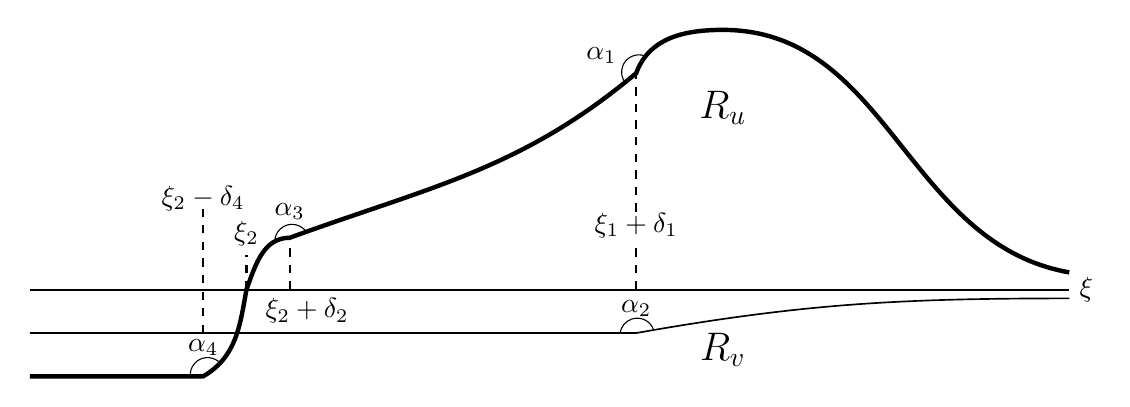
\begin{tikzpicture}[scale = 1.1]
\draw[thick](-6,0) -- (6,0) node[right] {$\xi$};
\draw [semithick] (-6,-0.5)--  (1,-0.5) to [out=10,in=180] (6,-0.1);
\draw [ultra thick] (-6, -1) -- (-4,-1) to [out=30, in=260] (-3.5,0)  to [out= 70, in=180] (-3,0.6) to [out=20, in=220] (1,2.5) to [out=70,in=180] (2,3)to [out=0,in=170] (6,0.2);
\node[below] at (1,1) {$\xi_{1}+\delta_1$};
%\node[below] at (0,-0.1) {$\xi_{\sigma}$};
\draw[dashed] [thick] (-3.5,0)-- (-3.5,0.4);
\node[below] at (-3.5,0.9) {$\xi_2$};
\draw[dashed] [thick] (-3,0.)-- (-3,0.6);
\node[above] at (-2.8,-0.5) {$\xi_2+\delta_2$};
\draw[dashed] [thick] (-4,-0.5)-- (-4,1);
\node[above] at (-4,0.8) {$\xi_2-\delta_4$};
\draw[dashed] [thick] (1,0)-- (1,0.55);
\draw[dashed] [thick] (1,0.9)-- (1,2.5);
\draw [thin] (1.2,-0.46) arc [radius=0.2, start angle=20, end angle= 170];
\node[above] at (1,-0.42) {$\alpha_2$};
\draw [thin] (-3.82,-0.83) arc [radius=0.2, start angle=50, end angle= 185];
\node[above] at (-4,-0.87) {$\alpha_4$};
\draw [thin] (-2.8,0.655) arc [radius=0.2, start angle=30, end angle= 175];
\node[above] at (-3,0.7) {$\alpha_3$};
\draw [thin] (1.1,2.7) arc [radius=0.2, start angle=70, end angle= 220];
\node[above] at (0.6,2.5) {$\alpha_1$};
%\draw [thin] (1.1,3.13) arc [radius=0.2, start angle=50, end angle= 180];
%\node[above] at (1,3.13) {$\alpha_2$};
%\node[above] at (2,1.5) {\Large{$v$}};
\node[above] at (2,1.8) {\Large{$R_u$}};
\node[above] at (2,-1) {\Large{$R_v$}};
%\node[below] at (1,-1.7) {Figure \ref{Figure prop}: $(R_u,R_v)$ to prove Proposition \ref{prop:0<b*<infty}.};
\end{tikzpicture}
\caption{$(R_u,R_v)$ to prove Proposition \ref{prop:0<b*<infty}.}\label{Figure prop}
\end{center}
\end{figure}


We consider $(R_u,R_v)(\xi)$ defined  as (see Figure \ref{Figure prop})
\begin{equation*}
(R_u,R_v)(\xi):=\begin{cases}
(\varepsilon_1\sigma(\xi) e^{-\lambda_u\xi},-\eta_1 e^{-\lambda_1\xi}),&\ \ \mbox{for}\ \ \xi\ge\xi_1+\delta_1,\\
(\varepsilon_2e^{\lambda_2\xi},-\delta_v),&\ \ \mbox{for}\ \ \xi_2+\delta_2\le\xi\le\xi_1+\delta_1,\\
(\varepsilon_3\sin(\delta_3(\xi-\xi_2)),-\delta_v),&\ \ \mbox{for}\ \ \xi_2-\delta_4\le\xi\le\xi_{2}+\delta_2,\\
(-\delta_u,-\delta_v),&\ \ \mbox{for}\ \ \xi\le\xi_2-\delta_4,
\end{cases}
\end{equation*}
where $\lambda_u:=\sqrt{1-a}$, $\xi_1>M_0$ and $\xi_2<-M_0$ are fixed points. Since $|R_u|,|R_v|\ll 1$, up to enlarging $M_0$, for all $\xi\in(-\infty,\xi_2]$, it holds
\bea\label{xi 2 b=0}
1-2W_*-a<-1+a+\rho,
\eea
with arbitrarily small $\rho>0$. We also set $0<\lambda_{1}<\lambda_u$ satisfies
\begin{equation}\label{condition on lambda 1 b=0}
d\lambda_1^2-2\sqrt{1-a}\,\lambda_1-r=:-C_0<0,
\end{equation}
and $\lambda_{2}$ satisfies
\begin{equation}\label{condition on lambda 2 b=0}
\lambda_2^2+2\sqrt{1-a}\,\lambda_2-3+a=:C_1>0.
\end{equation}
Here
$\varepsilon_{1,2,3}>0$ and $\eta_1>0$ make $(R_u,R_v)$ continuous on $\mathbb{R}$, while $\delta_{1,\cdots,4}>0$ will be determined later such that $(W_u,W_v)$ satisfies \eqref{super solution b=0}.  Moreover, we set
\bea\label{delta u v b=0}
\delta_u=\varepsilon_3\sin(\delta_3\delta_4)\quad\text{and}\quad \delta_v=\eta_1e^{-\lambda_1(\xi_1+\delta_1)},
\eea
which yield $(R_u,R_v)(\xi)$ are continuous on $\mathbb{R}$.

Next, we will divide the construction into several steps.

\noindent{\bf{Step 1}:} We consider $\xi\in[\xi_{1}+\delta_1,\infty)$ with $\xi_1>M_0$ and some small $\delta_1$ satisfying
\bea\label{cond delta 1 b=0}
0<\delta_1<\frac{1}{2(\lambda_2+\lambda_u)}.
\eea
In Step 1, we aim to verify that $(W_u,W_v)(\xi)=(U_*-R_u,2+R_v)(\xi)$, with
\beaa
(R_u,R_v)(\xi)=(\varepsilon_1\sigma(\xi)e^{-\lambda_u\xi},-\eta_1 e^{-\lambda_1\xi}),
\eeaa
satisfies \eqref{super solution b=0} by setting  $\delta_0$ sufficiently small.

Similar as the construction of $R_w(\xi)$ for single equation problem, we define
$$\sigma(\xi):=\frac{4}{\lambda_1^2}e^{-\frac{\lambda_1}{2}(\xi-\xi_1)}-\frac{4}{\lambda_1^2}+\frac{4}{\lambda_1}\xi-\frac{4}{\lambda_1}\xi_1$$
which satisfies 
$$\sigma(\xi_1)=0,\ \sigma'(\xi)=\frac{4}{\lambda_1}-\frac{2}{\lambda_1}e^{-\frac{\lambda_1}{2}(\xi-\xi_1)},\ \sigma''(\xi)=e^{-\frac{\lambda_1}{2}(\xi-\xi_1)},$$ 
and $\sigma(\xi)= O(\xi)$ as $\xi\to\infty$.
From \eqref{N3 b=0}, we have
\beaa
N_1[W_u,W_v]\le -e^{-\frac{\lambda_1}{2}(\xi-\xi_1)}R_u+R_u(2W_*-R_u+aR_v)-aW_*R_v.
\eeaa
Since $W_*(\xi)= O(\xi e^{-\lambda_u\xi})$ as $\xi\to\infty$ and  $0<\lambda_1<\lambda_u$, we obtain $N_1[W_u,W_v]\le 0$ for all $\xi\in[\xi_1+\delta_1,\infty)$ up to enlarging $M_0$ if necessary.


Next, we deal with the inequality of $N_2[W_u, W_v]$.
From \eqref{N4 b=0} and \eqref{condition on lambda 1 b=0}, we have
\begin{equation*}
N_2[W_u,W_v]\ge -C_0R_v-rR_vR_v-\delta_0r(1+R_v)W_*.
\end{equation*}
Since $0<\lambda_1<\lambda_u$ and $R_v<0$, by setting $\delta_0$ sufficiently small, then we have $N_2[W_u,W_v]\geq0$ for all $\xi\in[\xi_1+\delta_1,\infty)$ up to enlarging $M_0$ if necessary.

\medskip

\noindent{\bf{Step 2}:} We consider $\xi\in[\xi_{2}+\delta_2,\xi_1+\delta_1]$ with $\delta_1$ satisfying \eqref{cond delta 1 b=0}.
In this case, we have
$(R_u,R_v)(\xi)=(\varepsilon_2e^{\lambda_2\xi},-\delta_v)$
with $\lambda_2$ satisfying \eqref{condition on lambda 2 b=0} and $\delta_v$ defined as \eqref{delta u v b=0}. It is easy to see that $R_v(\xi)$ is continuous on $\xi=\xi_1+\delta_1$, and $\angle \alpha_2<180^{\circ}$ since 
$$R'_v((\xi_1+\delta_1)^+)>0=R'_v((\xi_1+\delta_1)^-).$$

On the other hand, we set
$$\varepsilon_2=\frac{\varepsilon_1\sigma(\xi_1+\delta_1)e^{-\lambda_u(\xi_1+\delta_1)}}{e^{\lambda_2(\xi_1+\delta_1)}}$$
such that $R_u(\xi)$ is continuous on $\xi=\xi_1+\delta_1$. Then, by some straightforward computations, we have
\beaa
&&R_u'((\xi_1+\delta_1)^+)=\varepsilon_1\sigma'(\xi_1+\delta_1)e^{-\lambda_u(\xi_1+\delta_1)}-\varepsilon_1\lambda_u\sigma(\xi_1+\delta_1)e^{-\lambda_u(\xi_1+\delta_1)},\\
&&R_u'((\xi_1+\delta_1)^-)=\lambda_2R_u(\xi_1+\delta_1).
\eeaa
Thus, $R_u'((\xi_1+\delta_1)^+)>R_u'((\xi_1+\delta_1)^-)$ %and $\angle \alpha_1<180^{\circ}$ are
is
equivalent to
$$(\lambda_2+\lambda_u)\sigma(\xi_1+\delta_1)<\sigma'(\xi_1+\delta_1),$$
which holds %since
since
\eqref{cond delta 1 b=0} and $\delta_1$ sufficiently small.


From \eqref{N3 b=0}, \eqref{condition on lambda 2 b=0}, and $R_v<0$, we have
\beaa
N_1[W_u,W_v]\le-C_1R_u+aW_*\delta_v.
\eeaa
Notice that, we can set $\eta_1\ll \varepsilon_1$ such that $\delta_v\ll|R_u|$ for all $\xi\in[\xi_2+\delta_2,\xi_1+\delta_1]$. Therefore, we have $N_1[W_u,W_v]\le 0$ for all $\xi\in[\xi_2+\delta_2,\xi_1+\delta_1]$.
On the other hand, from \eqref{N4 b=0} and $R_v<0$, we have
\beaa
N_2[W_u,W_v]=r\delta_v(1-\delta_v)-\delta_0r(1-\delta_v)(W_*-R_u).
\eeaa
Therefore, up to decreasing $\delta_0$ if necessary, we have $N_2[W_u,W_v]\ge 0$ for all
$\xi\in[\xi_2+\delta_2,\xi_1+\delta_1]$. Moreover, it is easy to see that $N_2[W_u,W_v]\ge 0$ for all $\xi\in(-\infty,\xi_1+\delta_1]$ as long as $\delta_0>0$ is sufficiently small since $W_*-R_u\leq 1$ in $\mathbb{R}$. Therefore, hereafter it suffices to prove the inequality of $N_1[W_u,W_v]$.



\medskip

\noindent{\bf{Step 3}:} We consider $\xi\in[\xi_{2}-\delta_4,\xi_2+\delta_2]$ with
\bea\label{cond delta 2 b=0}
\delta_2>\frac{1}{\lambda_2}.
\eea
In this case, we have $(R_u,R_v)=(\varepsilon_3\sin(\delta_3(\xi-\xi_2)),-\delta_v)$. We first set
$$\varepsilon_3=\frac{\varepsilon_2e^{\lambda_2(\xi_2+\delta_2)}}{\sin(\delta_2\delta_3)}$$
such that $R_u(\xi)$ is continuous on $\xi=\xi_2+\delta_2$.
Then, by some straightforward computations, we have
$$R_u'((\xi_2+\delta_2)^+)=\lambda_2R_u(\xi_2+\delta_2)\quad\text{and}\quad R_u'((\xi_2+\delta_2)^-)=\varepsilon_3\delta_3\cos(\delta_2\delta_3).$$
Thus, from $\frac{x\cos x}{\sin x}\to 1$ as $x\to 0$, 
$$R_u'((\xi_2+\delta_2)^+)>R_u'((\xi_2+\delta_2)^-),\ i.e.,\ \angle \alpha_3<180^{\circ},$$ 
follows by taking
%are equivalent to
$\delta_3$ sufficiently small and $\delta_2$ satisfying \eqref{cond delta 2 b=0}.

It suffices to only verify the inequality of $N_1[W_u,W_v]$. From \eqref{N3 b=0}, we have
\beaa
N_1[W_u,W_v]=\delta_3^2R_u-c^*\delta_3\varepsilon_3\cos(\delta_3(\xi-\xi_2))-R_u(1-a-2W_*+R_u-aR_v)-aW_*R_v.
\eeaa
For $\xi\in[\xi_2,\xi_2+\delta_2]$, we have
$$N_1[W_u,W_v]\le (\delta_3^2+1+a)\varepsilon_3\sin(\delta_2\delta_3)-c^*\delta_3\varepsilon_3\cos(\delta_2\delta_3)-aW_*R_v.$$
Note that, from $\frac{x\cos x}{\sin x}\to 1$ as $x\to 0$,
$$(\delta_3^2+1+a)\varepsilon_3\sin(\delta_2\delta_3)-c^*\delta_3\varepsilon_3\cos(\delta_2\delta_3)\le 0$$
is equivalent to $\delta_2<\frac{\delta_3c^*}{\delta_3^2+1+a}$ which holds since $\lambda_2$ in \eqref{cond delta 2 b=0} can be chosen arbitrarily large.
For $\xi\in[\xi_2-\delta_4,\xi_2]$, from $R_u\le 0$ and \eqref{xi 2 b=0}, up to enlarging $M_0$, we have
$$N_1[W_u,W_v]\le -c^*\delta_3\varepsilon_3\cos(\delta_2\delta_3)-aW_*R_v.$$
Then, by setting
\bea\label{delta 4 b=0}
0<\delta_4<\delta_2<\frac{\delta_3c^*}{\delta_3^2+1+a},
\eea
we have $N_1[W_u,W_v]\le 0$ for all $\xi\in[\xi_2-\delta_4,\xi_2+\delta_2]$ up to decreasing $\delta_0$ if necessary.

\medskip

\noindent{\bf{Step 4}:} We consider $\xi\in(-\infty,\xi_{2}-\delta_4]$. In this case, we have $(R_u,R_v)=(-\delta_u,-\delta_v)$.
From \eqref{delta u v b=0}, $R_u(\xi)$ is continuous on $\xi=\xi_2-\delta_4$. It is easy to see that 
$$R_u'((\xi_2-\delta_4)^+)>0=R_u'((\xi_2-\delta_4)^-)\ \ \text{and}\ \ \angle \alpha_4<180^{\circ}.$$
 Moreover, from \eqref{delta 4 b=0} and $\delta_v\ll R_u(\xi_2+\delta_2)$, we assert that $\delta_v\ll\delta_u$.

From \eqref{N3 b=0} and \eqref{xi 2 b=0}, we have
\beaa
N_1[W_u,W_v]=\delta_u(1-a-2W_*-\delta_u+a\delta_v)+aW_*\delta_v\le 0
\eeaa
since $\delta_v\ll\delta_u$. The construction of $(R_u,R_v)(\xi)$ is complete.

\medskip


\noindent{\bf{Step 5}}: We are ready to complete the proof of Proposition~\ref{prop:0<b*<infty}.
From Step 1 to Step 4, we are equipped with a super-solution $(W_u,W_v)(\xi)$.
Next, we consider the Cauchy problem \eqref{system2} with $b^*=0$.
By applying the same argument in the proof of Theorem \ref{th:threshold}, %for the case $0<b^*<1$,
we can reach a contradiction and thus $b^*=0$ is impossible. This completes the proof of Proposition \ref{prop:0<b*<infty}.
%we can finish the proof of Proposition \ref{prop:0<b*<infty}.
\end{proof}



Together with Proposition \ref{prop:0<b*<infty},
we immediately obtain Lemma~\ref{lm: existence b*}. 
\begin{lemma}\label{lm: existence b*}
For any $d>0$, $r>0$ and $a\in(0,1)$, there exists $0<b^*<\infty$  such that
\begin{equation*}
c_{LV}^{*}(b)=2\sqrt{1-a}\ \ \mbox{for}\ \ b\in(0,b^*]\ \  \mbox{and}\ \  c_{LV}^{*}(b)>2\sqrt{1-a} \ \ \mbox{for}\ \  b\in(b^*,+\infty).
\end{equation*}
\end{lemma}


\subsection{Construction of the super-solution}


\medskip

Now, we are ready to state the most important part of our argument. Let $(c_{LV}^{*}, U_*,V_*)$ be the minimal traveling wave of system \eqref{tw solution weak} with $b=b^*>0$
and $c_{LV}^{*}=c_{LV}^{*}(b^*)=2\sqrt{1-a}$.
Hereafter, for the simplicity we denote
\beaa
\lambda_u:=-\lambda_u^-(c_{LV}^{*}(b^*))>0,\ \lambda_v:=-\lambda_v^-(c_{LV}^{*}(b^*))>0,\
%\mu_u:=\mu_u^+(c^*(b^*))>0,\ \mu_v:=\mu_v^+(c^*(b^*))>0,
\eeaa
 where
$\lambda_u^-$ and $\lambda_v^-$ are defined in the Subsection~\ref{subsec:Asymp behavior}.

The first and most involved step is to show $(i)\Rightarrow (ii)$, i.e. if $b=b^*$, then $A=0$ in \eqref{1}. We shall use a contradiction argument to establish the following result.
\begin{proposition}\label{Prop-supersol-system}
Assume that {\bf(H)} holds. In addition, if
\bea\label{AS-U-infty-for-contradiction}
\lim_{\xi\rightarrow+\infty}\frac{U_{*}(\xi)}{\xi e^{-\lambda_u\xi}}=A_0\quad \mbox{for some $A_0>0$,}
\eea
then there exist two continuous functions $R_u(\xi)$ and $R_v(\xi)$
defined in $\mathbb{R}$ with
\bea\label{decay rate of Ru Rv}
R_u(\xi)=O(\xi e^{-\lambda_u\xi}),\quad R_v(\xi)=O(e^{-\lambda_u\xi}) \quad \mbox{as $\xi\to\infty$},
\eea
such that 
$$(W_u,W_v)(\xi):=\Big(\min\{(U_*-R_u)(\xi),1\},\max\{(V_*+R_v)(\xi),0\}\Big)$$
is a super-solution satisfying%forms a super-solution satisfying
\begin{equation}\label{tw super solution system}
\left\{
\begin{aligned}
&N_3[W_u,W_v]:=W_u''+2\sqrt{1-a}W_u'+W_u(1-W_u-aW_v)\le0,\ \mbox{a.e. in $\mathbb{R}$},\\
&N_4[W_u,W_v]:=dW_v''+2\sqrt{1-a}W_v'+rW_v(1-W_v-(b^*+\delta_0)W_u)\ge 0,\ \mbox{a.e. in $\mathbb{R}$},
%&W_u'\leq 0,\ W_v'\geq 0, \ \mbox{a.e. in $\mathbb{R}$}
\end{aligned}
\right.
\end{equation}
for all small $\delta_0>0$, where
$W'_u(\xi_0^{\pm})$
(resp. $W'_v(\xi_0^{\pm})$) exists and
\beaa
W'_u(\xi_0^+)\leq W'_u(\xi_0^-)\quad (resp.\, W'_v(\xi_0^+)\geq W'_v(\xi_0^-))
\eeaa
if  $W'_u$ (resp., $W'_v$) is not continuous at $\xi_0$.
%if $W'_u$ (resp., $W'_v$) is not continuous at $\xi_0$, then $W'_u(\xi_0^+)\leq W'_u(\xi_0^-)$
%(resp., $W'_v(\xi_0^+)\geq W'_v(\xi_0^-)$).
\end{proposition}


%We now show that for any given small $\sigma>0$,
%there exists two auxiliary functions $R_u(\xi)$ and $R_v(\xi)$ with
%\beaa
%R_u(\xi)=O(\xi e^{-\lambda_u\xi}),\quad R_v(\xi)=O(\xi e^{-\lambda_u\xi}) \quad \mbox{as $\xi\to\infty$},
%\eeaa
%such that $(W_u,W_v)(\xi):=(U_*-R_u,V_*+R_v)(\xi)$ forms a super-solution satisfying
%\begin{equation}\label{tw super solution case 2}
%\left\{
%\begin{aligned}
%&N_3[W_u,W_v]:=W_u''+(2\sqrt{1-a}+\sigma)W_u'+W_u(1-W_u-aW_v)\le0,\\
%&N_4[W_u,W_v]:=dW_v''+(2\sqrt{1-a}+\sigma)W_v'+rW_v(1-W_v-(b^*+\delta_0)W_u)\ge 0,\\
%&(W_u,W_v)(-\infty)=(1,0),\ (W_u,W_v)(+\infty)=(0,1),\\
%&W_u'< 0,\ W_v'> 0,
%\end{aligned}
%\right.
%\end{equation}
%for any sufficiently small $\delta_0>0$ which is independent of $\sigma$.



%%%%%%%%%%%%%%%%%%%%%%%%%%%%%%%%%%%%%%%%%%%%%%%%%%%%%%%%%%%%%%%
%By Lemma~\ref{lm: existence b*}, it suffices to prove \eqref{threshold rate}.
%For this, we assume by contradiction that \eqref{threshold rate} is not true. Then, by Lemma~\ref{lm: behavior around + infty}, we can find $A_0>0$ such that

In the following discussion, we divide the construction of
$(R_u,R_v)(\xi)$ into two subsections: $b^*\ge 1$ (the strong-weak competition case and the critical case); $0<b^*<1$ (the weak competition case).
%into 3 cases: Case (S1)(S2), Case (S3) and Case (S4).


\subsubsection{For the case $b^*\ge 1$}\label{sec:3-1}

\noindent

In this subsection, we always assume $b^*\ge 1$.
First, since
$(U_*,V_*)(-\infty)=(1,0)$ and
$(U_*,V_*)(+\infty)=(0,1)$, for any given small $\rho>0$, we can take $M_0>0$ sufficiently large such that
\bea\label{rho}
\begin{cases}
0< U_*(\xi)<\rho,\quad 1-\rho<V_*(\xi)<1&\quad\mbox{for all}\quad\xi\geq M_0,\\
0< V_*(\xi)<\rho,\quad 1-\rho<U_*(\xi)<1&\quad\mbox{for all}\quad\xi\leq -M_0.
\end{cases}
\eea

For $\xi$ being close to $\infty$, we have the following for later use. First,
due to \eqref{AS-U-infty-for-contradiction} and Lemma~\ref{lm: behavior around + infty}(ii), up to enlarging $M_0$ if necessary, we may assume that for some positive constant $A_0$,
\bea\label{U-M}
U_*(\xi) \leq 2A_0\xi e^{-\lambda_u\xi}\quad\mbox{for all}\quad\xi\geq M_0.
\eea
Moreover, we may also assume there exists $C_0>0$ such that
\bea\label{V-lower-bound-infty}
V_*(\xi) \geq 1-C_0\xi^2 e^{-\min\{\lambda_u,\lambda_v\}\xi}\quad
\mbox{for all}\quad\xi\geq M_0.
\eea
We also define
\bea\label{C1}
C_1:=\max_{\xi\in[M_0,\infty)}\Big|\frac{(d-2)(1-a)}{r}+1-2V_*(\xi)-(b^*+\delta_0)U_*(\xi)\Big|>0.
\eea


%\red{Let $\xi_1>M_0$ be a large positive point and $\xi_2<-M_0$ be a large negative point.}
We now define $(R_u,R_v)(\xi)$ as (see Figure~\ref{Figure:b>1})
\begin{equation*}
(R_u,R_v)(\xi):=\begin{cases}
(\varepsilon_1\sigma(\xi) e^{-\lambda_u\xi},\eta_1 (\xi-\xi_1)e^{-\lambda_u\xi}),&\ \ \mbox{for}\ \ \xi_1+\delta_1\le\xi,\\
(\varepsilon_2\sin(\delta_2(\xi-\xi_1+\delta_3)),\eta_2e^{\lambda_{1}\xi}),&\ \ \mbox{for}\ \ \xi_1-\delta_4\le\xi\le\xi_{1}+\delta_1,\\
(-\varepsilon_3,\eta_2e^{\lambda_{1}\xi}),&\ \ \mbox{for}\ \ \xi_2+\delta_5\le\xi\le\xi_1-\delta_4,\\
(-\varepsilon_4(-\xi)^{\theta}[1-U_*(\xi)],\eta_3\sin(\delta_6(\xi-\xi_2))),&\ \ \mbox{for}\ \ \xi_2-\delta_7\le\xi\le\xi_2+\delta_5,\\
(-\varepsilon_4(-\xi)^{\theta}[1-U_*(\xi)],-\eta_4(-\xi)^{\theta}V_*(\xi),&\ \ \mbox{for}\ \ \xi\le\xi_2-\delta_7,
\end{cases}
\end{equation*}
where
$0<\theta<1$, and $\lambda_{1}>0$ is fixed such that
\begin{equation}\label{condition on lambda 1 system}
d\lambda_1^2+2\sqrt{1-a}\,\lambda_1-r(2+b^*)>0\ \ {\rm and}\ \ \lambda_1>\frac{2r(b^*+1)}{\sqrt{1-a}}.
\end{equation}
Here $\xi_1>M_0$, $\xi_2<-M_0$, $\varepsilon_{i=1,\cdots,4}>0$ and $\eta_{j=1,\cdots,4}>0$, $\delta_{k=1,\cdots,7}>0$,
%make $(W_u,W_v)$ be continuous functions on $\mathbb{R}$
and $\sigma(\xi)$ will be determined later.

%such that $(W_u,W_v)$ satisfies \eqref{tw super solution system} for $\xi\in\mathbb{R}$.

\begin{figure}
\begin{center}
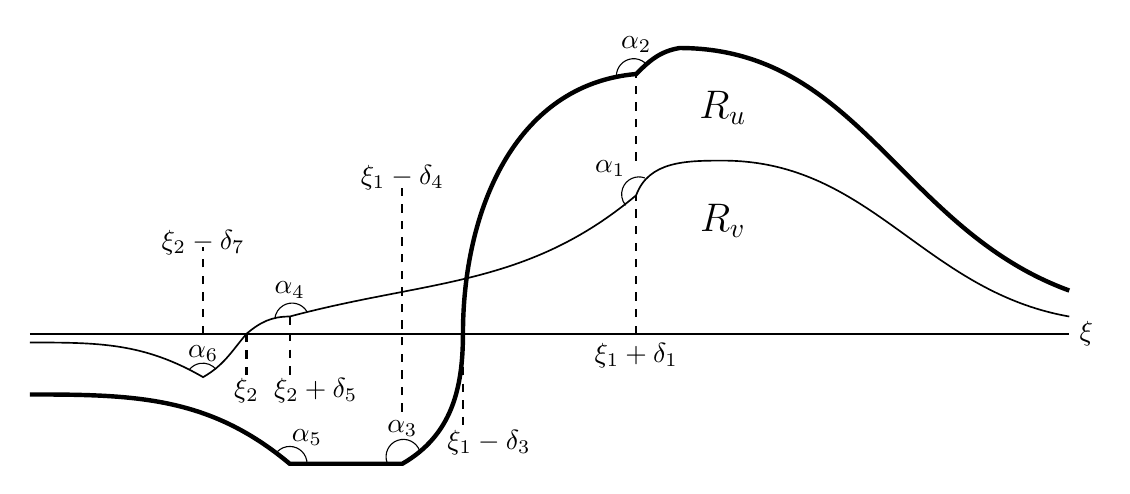
\begin{tikzpicture}[scale = 1.1]
\draw[thick](-6,0) -- (6,0) node[right] {$\xi$};
\draw [ultra thick] (-6,-0.7)to [out=0,in=140] (-3,-1.5) -- (-1.7,-1.5)  to [out=30,in=270]   (-1,0)  to [out=90,in=185]  (1,3) to [out=45,in=190] (1.5,3.3) to [out=0,in=160] (6,0.5);
\draw [semithick] (-6, -0.1) to [ out=0, in=150] (-4,-0.5) to [out=30, in=230] (-3.5,0)  to [out= 40, in=180] (-3,0.2) to [out=15, in=220] (1,1.6) to [out=70,in=180] (2,2)to [out=0,in=170] (6,0.2);
\node[below] at (1,0) {$\xi_{1}+\delta_1$};
%\node[below] at (0,-0.1) {$\xi_{\sigma}$};
\draw[dashed] [thick] (-3.5,0)-- (-3.5,-0.5);
\node[below] at (-3.5,-0.4) {$\xi_2$};
\draw[dashed] [thick] (-3,0.2)-- (-3,-0.5);
\node[below] at (-2.7,-0.4) {$\xi_2+\delta_5$};
\draw[dashed] [thick] (-4,0)-- (-4,1);
\node[above] at (-4,0.8) {$\xi_2-\delta_7$};
\draw[dashed] [thick] (1,0)-- (1,1.6);
\draw[dashed] [thick] (1,2)-- (1,3);
\draw[dashed] [thick] (-1,0)-- (-1,-1.1);
\draw[dashed] [thick] (-1.7,-0.9)-- (-1.7,1.7);
\node[above] at (-1.7,1.55) {$\xi_1-\delta_4$};
%\node[below] at (-2.5,-0.2) {$\xi_2$};
%\draw[dashed] [thick] (-2.5,-0.3)-- (-2.5,0.3);
%\draw[dashed] [thick] (-2.5,-0.7)-- (-2.5,-1);
\node[below] at (-0.7,-1) {$\xi_1-\delta_3$};
\draw [thin] (-3.85,-0.41) arc [radius=0.2, start angle=40, end angle= 140];
\node[above] at (-4,-0.43) {$\alpha_6$};
\draw [thin] (-2.8,-1.5) arc [radius=0.2, start angle=0, end angle= 135];
\node[above] at (-2.8,-1.4) {$\alpha_5$};
\draw [thin] (-2.8,0.255) arc [radius=0.2, start angle=30, end angle= 175];
\node[above] at (-3,0.3) {$\alpha_4$};
\draw [thin] (-1.5,-1.35) arc [radius=0.2, start angle=20, end angle= 200];
\node[above] at (-1.7,-1.3) {$\alpha_3$};
\draw [thin] (1.1,1.8) arc [radius=0.2, start angle=70, end angle= 220];
\node[above] at (0.7,1.7) {$\alpha_1$};
\draw [thin] (1.1,3.13) arc [radius=0.2, start angle=50, end angle= 180];
\node[above] at (1,3.13) {$\alpha_2$};
%\node[above] at (2,1.5) {\Large{$v$}};
\node[above] at (2,2.3) {\Large{$R_u$}};
\node[above] at (2,1) {\Large{$R_v$}};
%\node[below] at (1,-2.3) {Figure~\ref{Figure:b>1}: $(R_u,R_v)$ for the case $b^*\ge 1$.};
\end{tikzpicture}
\caption{$(R_u,R_v)$ for the case $b^*\ge 1$.}\label{Figure:b>1}
\end{center}
\end{figure}




\medskip



%On the other hand, due to Lemma \ref{lm: behavior around - infty b=1}, we may assume
%\bea\label{U-V at -infty}
%1-U_*(\xi)\approx\tau_u(\xi)\quad\text{and}\quad V_*(\xi)\approx \tau_v(\xi)\quad\text{for}\quad\xi\le-M_0,
%\eea
%with $(\tau_u,\tau_v)(\xi)$ satisfies %\eqref{system tau u v}.

%By shifting the coordinates, we may assume $\xi_1<M$ such that
%statment (1) and (3) holds
%for all $\xi\ge \xi_1$.

Next, we  divide the proof into several steps.
\medskip

\noindent{\bf{Step 1}:} We consider $\xi\in[\xi_{1}+\delta_1,\infty)$ with $\xi_1>M_0$ ($M_0$ is defined in \eqref{rho}) and  some small $\delta_1$ satisfying
\bea\label{cond delta 1}
0<\delta_1<\frac{1}{\lambda_u+\lambda_1}\quad\text{and}\quad\frac{1}{\lambda_u}+\frac{3}{\lambda_u}(1-e^{-\frac{\lambda_u\delta_1}{2}})-2\delta_1>0.
\eea
In Step 1, we aim to verify that $(W_u,W_v)(\xi)=(U_*-R_u,V_*+R_v)(\xi)$ with
\beaa
(R_u,R_v)(\xi)=(\varepsilon_1\sigma(\xi)e^{-\lambda_u\xi},\eta_1(\xi-\xi_{1}) e^{-\lambda_u\xi}),
\eeaa
satisfies \eqref{tw super solution system} by setting $\varepsilon_1$ relatively smaller than $A_0$, $\eta_1$ relatively smaller than $\varepsilon_1$, and
\bea\label{cond delta 0 system case 1}
0<\delta_0<\frac{\varepsilon_1rb^*-2rC_1\lambda_u\eta_1-2|1-d|\lambda^2_u\eta_1}{rA_0\lambda_u},
\eea
where $C_1$ is defined in \eqref{C1}.

We define
$$\sigma(\xi):=\frac{4}{\lambda_u^2}e^{-\frac{\lambda_u}{2}(\xi-\xi_1)}-\frac{4}{\lambda_u^2}+\frac{4}{\lambda_u}\xi-\frac{4}{\lambda_u}\xi_1$$
which satisfies 
$$\sigma(\xi_1)=0,\ \sigma'(\xi)=\frac{4}{\lambda_u}-\frac{2}{\lambda_u}e^{-\frac{\lambda_u}{2}(\xi-\xi_1)},\ \sigma''(\xi)=e^{-\frac{\lambda_u}{2}(\xi-\xi_1)},$$ 
and $\sigma(\xi)= O(\xi)$ as $\xi\to\infty$.
Therefore, $R_u$ satisfies \eqref{decay rate of Ru Rv}.
Moreover, by some  straightforward computations, we obtain $R'_v((\xi_1+\delta_1)^+)>0$, while
$R'_u((\xi_1+\delta_1)^+)>0$ follows from \eqref{cond delta 1}.

Recall that, $(U_*,V_*)$ is the minimal traveling wave satisfying \eqref{tw solution weak} with $c=2\sqrt{1-a}$.
By some  straightforward computations,  we have
$$N_3[W_u,W_v]=-\varepsilon_1\sigma''(\xi)e^{-\lambda_u\xi}-R_u(a-2U_*+R_u-aV_*-aR_v)-aR_vU_*,$$
and
\begin{equation*}
\begin{aligned}
N_4[W_u,W_v] = & rR_v\Big[\frac{(d-2)(1-a)}{r}+1-2V_*-R_v-(b^*+\delta_0)U_*+(b^*+\delta_0)R_u\Big]\\
&+2(1-d)\lambda_u\eta_1e^{-\lambda_u\xi}+rV_*[(b^*+\delta_0)R_u-\delta_0U_*].
\end{aligned}
\end{equation*}
 Then, from \eqref{U-M} and \eqref{V-lower-bound-infty}, by setting  $\varepsilon_1>0$ and $\eta_1>0$ relatively small to $A_0$,
for all $\xi\in[\xi_1+\delta_1,\infty)$, it holds
$$a-2U_*+R_u-aV_*-aR_v = o(e^{-\frac{\lambda_u}{2}\xi}).$$
Then, up to enlarging $\xi_1$ if necessary, since $R_v>0$, we obtain that $N_3[W_u,W_v]\leq0$
for all $\xi\in[\xi_1+\delta_1,\infty)$.

Next, we deal with the inequality of $N_4[W_u, W_v]$.
%\red{First, we denote
%\[
%C_1:=\max_{\xi\in[M_0,\infty)}\Big|\frac{(d-2)(1-a)}{r}+1-2V_*-(b^*+\delta_0)U_*\Big|>0.
%\]
%} Then,
For $\xi\in[\xi_1+\delta_1,\infty)$, from \eqref{rho} and \eqref{C1}, we have
\begin{equation*}
N_4[W_u,W_v]\geq -rR_v(C_1+R_v)+2(1-d)\lambda_u\eta_1e^{-\lambda_u\xi}+r(1-\rho)(b^*+\delta_0)R_u-r\delta_0U_*.
\end{equation*}
From the definition of $\sigma(\xi)$, we can find a $M_1>\xi_1$ such that $\sigma(\xi)\approx \frac{4}{\lambda_u}\xi$.
In view of \eqref{U-M} and 
$$2(1-d)\lambda_u\eta_1e^{-\lambda_u\xi}=o(R_u)\ \ \text{as} \ \ \xi\to\infty,$$
by further choosing ${\eta_1}/{\varepsilon_1}$ sufficiently small and $\delta_0$ satisfying \eqref{cond delta 0 system case 1}, we have $N_4[W_u,W_v]\geq0$
for $\xi\geq M_1$. For $\xi\in[\xi_1+\delta_1,M_1]$, by choosing ${\eta_1}/{\varepsilon_1}$ sufficiently small, we have
$$-rR_v(C_1+R_v)+2(1-d)\lambda_u\eta_1e^{-\lambda_u\xi}+r(1-\rho)(b^*+\delta_0)R_u> 0.$$
Since $U_*$ is bounded on $[\xi_1+\delta_1,M_1]$, by setting $\delta_0$ sufficiently small, then we have $N_4[W_u,W_v]\geq0$ for all $\xi\geq \xi_1+\delta_1$.



%On the other hand, for $\xi\in[\xi_1+\delta_1,M]$, since $R_u>0$, we can re-choose $\eta_1>0$ relatively smaller than $\varepsilon_1$ and $\delta_0$ sufficiently small such that $N_4[W_u,W_v]\geq0$ for  $\xi\geq [\xi_1+\delta_1,M]$.

\medskip

\noindent{\bf{Step 2:}} We consider $\xi\in[\xi_1-\delta_4,\xi_1+\delta_1]$ with $\delta_1$ satisfying \eqref{cond delta 1} and $\delta_4>0$ will be determined later. In this case, we have
$$(R_u,R_v)(\xi):=(\varepsilon_2\sin(\delta_2(\xi-\xi_1+\delta_3)),\eta_2e^{\lambda_{1}\xi})$$
with $0<\delta_2<1$ sufficiently small,
\bea\label{cond delta 4}
0<\delta_3<\delta_4\quad\text{satisfying}\quad|\delta_3-\delta_4|\ll 1,
\eea
 and
\bea\label{cond delta 3 4}
\delta_1+\delta_3=\frac{\sqrt{1-a}}{2+a}<\frac{\pi}{2\delta_2}.
\eea


We first verify the following claim: %as follows:
\begin{claim}\label{cl: alpha 1 aplha 2}
There exist %$\xi_2<\xi_1$, $\delta_1>0$ and
$\varepsilon_2>0$ and $\eta_2>0$ sufficiently small
such that
\beaa
&&R_u((\xi_{1}+\delta_1)^+)=R_u((\xi_{1}+\delta_1)^-),\quad R_v((\xi_{1}+\delta_1)^+)=R_v((\xi_{1}+\delta_1)^-),\\ &&\angle\alpha_1<180^{\circ}, \quad\text{and}\quad \angle\alpha_2<180^{\circ},
\eeaa
provided that  $\delta_1,\delta_3$ satisfy \eqref{cond delta 1} and \eqref{cond delta 3 4},  and $\delta_2$ is sufficiently small.
\end{claim}
\begin{proof}
By some  straightforward computations, we have
\beaa
&&R_u((\xi_{1}+\delta_1)^+)=\varepsilon_1\sigma(\xi_1+\delta_1)e^{-\lambda_u(\xi_{1}+\delta_1)},\quad R_u((\xi_{1}+\delta_1)^-)=\varepsilon_2\sin(\delta_2(\delta_1+\delta_3)),\\
&&R'_u((\xi_{1}+\delta_1)^+)=\varepsilon_1\sigma'(\xi_1+\delta_1)e^{-\lambda_u(\xi_{1}+\delta_1)}-\lambda_uR_u(\xi_{1}+\delta_1),\\
&&R'_u((\xi_{1}+\delta_1)^-)=\varepsilon_2\delta_2\cos(\delta_2(\delta_1+\delta_3)).
\eeaa
We first choose %sufficient small and
$\varepsilon_2=\varepsilon_1\sigma(\xi_1+\delta_1)e^{-\lambda_u(\xi_{1}+\delta_1)}/\sin(\delta_2(\delta_1+\delta_3))$ such that
\beaa
R_u((\xi_{1}+\delta_1)^+)=R_u((\xi_{1}+\delta_1)^-).
\eeaa
Then, by applying \eqref{cond delta 3 4} and the fact $\frac{x\cos x}{\sin x}\to 1$ as $x\to 0$, we have 
$$R'_u((\xi_{1}+\delta_1)^+)-R'_u((\xi_{1}+\delta_1)^-)>0$$
 is equivalent to
\beaa
\frac{2}{\lambda_u}+\frac{2}{\lambda_u}(1-e^{-\frac{\lambda_u\delta_1}{2}})>(\frac{1}{\delta_1+\delta_3}+\lambda_u)\sigma(\xi_1+\delta_1),
\eeaa
which holds since $\sigma(\xi_1+\delta_1)\to 0$ as $\delta_1\to 0$ and \eqref{cond delta 3 4}. It follows that $\angle\alpha_1<180^{\circ}$.



On the other hand, by some  straightforward computations, we have
\beaa
&&R_v((\xi_{1}+\delta_1)^-)=\eta_2e^{\lambda_1(\xi_{1}+\delta_1)},\ R_v((\xi_{1}+\delta_1)^+)=\eta_1\delta_1e^{-\lambda_u(\xi_{1}+\delta_1)},\\
&&R'_v((\xi_{1}+\delta_1)^-)=\lambda_1\eta_2e^{\lambda_1(\xi_{1}+\delta_1)},\ R'_v((\xi_{1}+\delta_1)^+)=\eta_1(1-\delta_1\lambda_u)e^{-\lambda_u(\xi_{1}+\delta_1)},
\eeaa
where $\lambda_1$ satisfies \eqref{condition on lambda 1 system}.
We take
\beaa
\eta_2=\eta_1\delta_1e^{-(\lambda_u+\lambda_1)(\xi_{1}+\delta_1)}>0,
\eeaa
which implies $R_v((\xi_{1}+\delta_1)^-)=R_v((\xi_{1}+\delta_1)^+)$. Then, from \eqref{cond delta 1}, we have
\beaa
R_v'((\xi_{1}+\delta_1)^+)-R_v'((\xi_{1}+\delta_1)^-)=\eta_1e^{-\lambda_u(\xi_1+\delta_1)}(1-\delta_1\lambda_u-\delta_1\lambda_1)>0,
\eeaa
which yields that $\angle\alpha_2<180^{\circ}$.
The proof of Claim \ref{cl: alpha 1 aplha 2} is complete.
\end{proof}

To finish Step 2, it suffices to take a small $\delta_2>0$ and suitable $0<\delta_3<\delta_4$ such that
\bea\label{goal: step 3}
N_3[W_u,W_v]\leq 0\quad\text{and}\quad N_4[W_u,W_v]\geq 0\quad \mbox{for}\quad \xi\in[\xi_1-\delta_4,\xi_1+\delta_1].
\eea
By some  straightforward computations, for $\xi\in[\xi_2-\delta_3,\xi_1+\delta_1]$ we have
\beaa
N_3[W_u,W_v]&=&-2\sqrt{1-a}\delta_2\varepsilon_2\cos(\delta_2(\xi-\xi_1+\delta_3))-a(U_*-R_u)R_v\\
&&-R_u(1-\delta_2^2-2U_*+R_u-aV_*),\\
N_4[W_u,W_v]&=&R_v\Big[d\lambda_1^2+2\sqrt{1-a}\lambda_1+r[1-2V_*-R_v-(b^*+\delta_0)(U_*-R_u)]\Big]
            \\&&+rV_*[(b^*+\delta_0)R_u-\delta_0U_*].
\eeaa
%For $\xi\in[\xi_1,\xi_1+\delta_2]$, since $R_u>0$, from  \eqref{mu_1 v}, one has $N_4[W_u,W_v]\ge 0$, up to decrease $\varepsilon_0$ if it is necessary.  Moreover, by applying the same argument in Step 2 of Case 1, one also has $N_3[W_u,W_v]\le 0$, up to decrease $\delta_2$ if it is necessary.
To estimate $N_3[W_u,W_v]$,
we consider $\xi\in[\xi_1-\delta_3,\xi_1+\delta_1]$ and $\xi\in[\xi_1-\delta_4,\xi_1-\delta_3]$ separately as follows:
\begin{itemize}
\item For $\xi\in[\xi_1-\delta_3,\xi_1+\delta_1]$, we have
$$0\le R_u(\xi)\le \varepsilon_2\sin(\delta_2(\delta_1+\delta_3))$$
 and $R_v(\xi)\geq0$.
%\leq R_u(\xi_1+\delta_1)=\varepsilon_2\sin(\delta_2(\xi_1-\xi_2+\delta_1))$.
Then, from \eqref{cond delta 3 4},  we have
\beaa
N_3[W_u,W_v]&\leq& -R_u({\xi})\Big(2\sqrt{1-a}\frac{\delta_2\cos(\delta_2(\delta_1+\delta_3))}{\sin(\delta_2(\delta_1+\delta_3))}+1-\delta_2^2-2U_*-aR_v-aV_*\Big)\\
&\le & -R_u({\xi})\Big(\frac{2\sqrt{1-a}}{\delta_1+\delta_3}-2-a\Big)\leq 0,
\eeaa
provided that $\delta_2$ is sufficiently small.

\item For $\xi\in[\xi_1-\delta_4,\xi_1-\delta_3]$, we have $R_u(\xi)\leq 0$, $R'_u(\xi)\geq 0$, and $R_v(\xi)\ge 0$.
Note that, $|R_u(\xi)|\ll R_v(\xi)$ for $\xi\in[\xi_1-\delta_4,\xi_1-\delta_3]$ and
\bea\label{delta3-4 to 0}
\max_{\xi\in[\xi_1-\delta_4,\xi_1-\delta_3]}|R_u(\xi)|\to 0\quad\text{as}\quad|\delta_3-\delta_4|\to 0.
\eea
Then, since $a(U_*-R_u)R_v> 0$, we have
%$$-2\sqrt{1-a}\delta_2\varepsilon_2\cos(\delta_2(\xi-\xi_2))=-\frac{2\sqrt{1-a}}{\xi-\xi_2}R_u< (1+R_u)R_u\quad\text{as} \quad\delta_2(\xi-\xi_2)\to 0,$$
%there exist $\xi_2$ close to $\xi_1$ and $\delta_5$ very small such that $N_3[W_u,W_v]\le 0$ for all $\xi\in[\xi_2,\xi_1]$.
\beaa
N_3[W_u,W_v]\leq -a(U_*-R_u)R_v-R_u(1-\delta_2^2-2U_*+R_u-aV_*)\leq 0,
\eeaa
provided $|\delta_3-\delta_4|>0$ is chosen sufficiently small.
\end{itemize}
From the above discussion, we asset that 
$$N_3[W_u,W_v]\leq 0\ \ \text{for}\ \ \xi\in[\xi_1-\delta_4,\xi_1+\delta_1],$$
provided that $\delta_1, \delta_3, \delta_4$ satisfy \eqref{cond delta 4} and \eqref{cond delta 3 4}, and
$\delta_2$ is small enough.

On the other hand, thanks to \eqref{condition on lambda 1 system}, we have
\bea\label{N4-Step3}
N_4[W_u,W_v]&\geq&R_v\Big[r(2+b^*)+r[1-2V_*-R_v-(b^*+\delta_0)(U_*-R_u)]\Big]
            \\&&+rV_*[(b^*+\delta_0)R_u-\delta_0U_*]\notag\\
           &\geq&  \frac{r}{2}R_v+rV_*[(b^*+\delta_0)R_u-\delta_0U_*].\notag
\eea
Note that $R_u(\xi)\geq0$ for $\xi\in[\xi_1-\delta_3,\xi_1+\delta_1]$; $R_u(\xi)<0$ but satisfies \eqref{delta3-4 to 0} for $\xi\in[\xi_1-\delta_4,\xi_1-\delta_3)$.
Consequently, we assert that
$$N_4[W_u,W_v]\ge 0\ \ \text{for all}\ \ \xi\in[\xi_2-\delta_3,\xi_1+\delta_1]$$
 up to decreasing $|\delta_3-\delta_4|$ and $\delta_0$ if necessary.
This completes the proof of \eqref{goal: step 3}, and Step 2 is finished.

\medskip


%Next, let us fix $\xi_2$ sufficiently close to $-\infty$.
%Since $U_*(-\infty)=1$
%and $R_u(\xi)=-\varepsilon_2\sin(\delta_2(\delta_3-\delta_4))$ for all $\xi\leq \xi_1-\delta_4$,
%we can take $\xi_0\gg1$ such that $U(\xi)-R_u=U(\xi)+\varepsilon_2\sin(\delta_2(\delta_3-\delta_4))>1$  for all $\xi<-\xi_0$ and then
%\bea\label{xi0}
%W_u(\xi):=\min\{U_*(\xi)-R_u(\xi),1\}=1\quad \mbox{for all $\xi<-\xi_0$}.
%\eea
%Hereafter, let us fix $\xi_2$ close to $-\infty$ such that $\xi_2+\delta_5<\min\{-\xi_0,-M_0\}$, where $M_0$ is defined in \eqref{rho}. Therefore, we have
%\bea\label{Wu=1}
%W_u(\xi)=1\quad \mbox{for all $\xi\leq \xi_2+\delta_5$}
%\eea

\noindent{\bf{Step 3:}} We consider $\xi\in[\xi_2+\delta_5,\xi_1-\delta_4]$ for some $\delta_5>0$ such that $\xi_2+\delta_5<-M_0$ and satisfies
\bea\label{cond delta 5}
\delta_5>\frac{1}{\lambda_1}\quad\text{and}\quad \Big|\delta_5-\frac{1}{\lambda_1}\Big|\ \text{is sufficiently small}.
\eea

In this case, we have
\beaa
(R_u,R_v)(\xi)=(-\varepsilon_3,\eta_2e^{\lambda_1\xi}).
\eeaa

First, we choose $\varepsilon_3=R_u(\xi_1-\delta_4)$ such that $R_u(\xi)$ is continuous at $\xi=\xi_1-\delta_4$.
Clearly, by setting $|\delta_3-\delta_4|$ very small as in Step 2, we have 
$$R'_u((\xi_1-\delta_{4})^+)>0=R'_u((\xi_1-\delta_{4})^-),\  i.e.,\  \angle\alpha_3<180^{\circ}.$$


By some straightforward computations, we have
\beaa
N_3[W_u,W_v]=-R_u(1-2U_*+R_u-a(V_*+R_v))-aU_*R_v,
\eeaa
and $N_4[W_u,W_v]$ satisfies \eqref{N4-Step3}.
Note that, $|\delta_3-\delta_4|\to0$ implies that $\varepsilon_3\to 0$, and $|R_v(\xi)|$
does not depend on $|\delta_3-\delta_4|$.
It follows that 
$$|R_u(\xi)|\ll |R_v(\xi)|\ \ \text{for all}\ \ \xi\in[\xi_2+\delta_5,\xi_1-\delta_4]$$
up to decreasing $|\delta_3-\delta_4|$ if necessary. Also, we have $\min_{\xi\in(-\infty,\xi_1-\delta_4]}U_*(\xi)>0$. Therefore,
we see that 
$$N_3[W_u,W_v]\leq 0\ \ \text{for}\ \ \xi\in[\xi_2+\delta_5,\xi_1-\delta_4]$$
by taking $|\delta_3-\delta_4|$ sufficiently small.
On the other hand, by using the same process in Step 2, we see that 
$$N_4[W_u, W_v]\geq 0\ \ \text{for}\ \ \xi\in[\xi_2+\delta_5,\xi_1-\delta_4]$$
up to decreasing $|\delta_3-\delta_4|$ and $\delta_0$ is necessary. Thus, Step 3 is finished.

\medskip

\noindent{\bf{Step 4:}} We consider $\xi\in[\xi_2-\delta_7,\xi_2+\delta_5]$.
In this case, we have
\beaa
(R_u,R_v)(\xi)=\Big(-\varepsilon_4(-\xi)^{\theta}[1-U_*(\xi)],\eta_3\sin(\delta_6(\xi-\xi_2))\Big),
\eeaa
where $\theta\in(0,1)$ is fixed,
while $\varepsilon_4>0$, $\eta_3>0$,
$\delta_6>0$, and $\delta_7>0$ are determined below.

%In view of Lemma~\ref{lem:AS-infty:b=1} and Lemma~\ref{lem:AS-infty:b>1}, we see that $1-U$ decays to zero either exponentially or algebraically as $\xi\to-\infty$. Therefore,
%without loss of generality, we may assume that
%\beaa
%(-\xi)^{\theta}[1-U_*(\xi)]<\varepsilon_3\quad \mbox{for all $\xi\leq -M_0$.}
%\eeaa

%Note that, $R_u(\xi)\le 0$ on $(-\infty,\xi_2+\delta_5]$ since \blue{$\xi_2+\delta_5\le -M_0$}.

We first choose
\bea\label{epsilon4}
\varepsilon_4=\frac{\varepsilon_3}{(-\xi_2-\delta_5)^{\theta}[1-U_*(\xi_2+\delta_5)]}
\eea
such that $R_u(\xi)$ is continuous at $\xi=\xi_2+\delta_5$,
where $\varepsilon_3$ and $\delta_5$ are fixed in Step 3.
Then, from the behavior of $1-U_*$ for both cases $b^*>1$ and $b^*=1$ as $\xi\to-\infty$ in the Appendix, we may assume that $R'_u(\xi)<0$ for all $\xi\leq \xi_2+\delta_5$. In particular,
%Lemma \ref{lm: behavior around - infty b=1},
we have
\beaa
R'_u((\xi_2+\delta_5)^+)=0>R'_u((\xi_2+\delta_5)^-),
\eeaa
and thus $\angle\alpha_5<180^{\circ}$.
Next, we verify the following claim to obtain the continuity of $R_v$ at $\xi_2+\delta_5$ and the right angle of $\alpha_6$:
\begin{claim}\label{cl 5}
For any $\delta_5$ with $\delta_5>\frac{1}{\lambda_1}$, there exist
% $\gamma_6=\frac{\eta_5}{\varepsilon_5}$, such that $R_v(\xi_3+)=R_v(\xi_3-)$ and $\angle\alpha_4<180^{\circ}$.
$\eta_3>0$ and small $\delta_6>0$
such that $R_v(\xi)$ is continuous at $\xi=\xi_2+\delta_5$ and $\angle\alpha_6<180^{\circ}$.
\end{claim}
\begin{proof}
First, we  take
\bea\label{eta4}
\eta_3= \frac{\eta_2e^{\lambda_1(\xi_2+\delta_5)}}{\sin(\delta_5\delta_6)}>0
\eea
such that $R_v((\xi_2+\delta_5)^+)=R_v((\xi_2+\delta_5)^-)$.

By some straightforward computations, we have
$R'_v((\xi_2+\delta_5)^+)=\lambda_1\eta_2e^{\lambda_1(\xi_2+\delta_5)}$, and from \eqref{eta4},
\beaa
R'_v((\xi_2+\delta_5)^-)=\eta_3\delta_6\cos(\delta_5\delta_6)=\eta_2e^{\lambda_1(\xi_2+\delta_5)}\frac{\delta_6\cos(\delta_5\delta_6)}{\sin(\delta_5\delta_6)},
\eeaa
% We first let $R_v(\xi_3+)=R_v(\xi_3-)$. Then, since $\sin(\delta_3(\xi_3-\xi_4))=\delta_3(\xi_3-\xi_4)\cos(\delta_3(\xi_3-\xi_4))$ as $\delta_3\to 0$, $R'_v(\xi_3+)>R'_v(\xi_3-)$ is equivalent to $(\xi_3-\xi_4)>\frac{1}{\mu_1}$.
which yields that
$$R'_v((\xi_2+\delta_5)^-)\rightarrow \eta_2e^{\lambda_1(\xi_2+\delta_5)}/\delta_5\quad\text{as}\quad \delta_6\to0.$$
Thus, $R'_v((\xi_2+\delta_5)^+)>R'_v((\xi_2+\delta_5)^-)$ is equivalent to $\delta_5>\frac{1}{\lambda_1}$ by setting $\delta_6$ sufficiently small.
This completes the proof of Claim~\ref{cl 5}.
\end{proof}



Next, we prove the following claim to determine $\delta_7$.
Note that the choice of $\delta_7$ is rather technical and crucial when we prove the differential inequalities later.

\begin{claim}\label{cl 6}
There exists $0<\delta_7\le \delta_5$ such that 
$$R_v(\xi_2-\delta_7)=-\varepsilon_4(-\xi_2+\delta_7)^{\theta}V_*(\xi_2-\delta_7)$$ 
and
\bea\label{claim3.6}
-\varepsilon_4(-\xi)^{\theta}V_*(\xi)<R_v(\xi)<0\quad\text{for all}\quad \xi\in(\xi_2-\delta_7,\xi_2).
\eea
\end{claim}
\begin{proof}
Recall from Step 3 and \eqref{epsilon4}
that 
$$R_v(\xi_2+\delta_5)\gg \varepsilon_3=\varepsilon_4(-\xi_2-\delta_5)^{\theta}[1-U_*(\xi_2+\delta_5)].$$
Together with Lemma~\ref{lem:AS-infty:b>1} (if $b^*>1$) and Lemma~\ref{lem:AS-infty:b=1} (if $b^*=1$), we may assume that
%and decreasing $\delta_7$,
\bea\label{Rv>V}
R_v(\xi_2+\delta_5)>\varepsilon_4(-\xi_2-\delta_5)^{\theta}V_*(\xi_2+\delta_5),
\eea
if necessary, we may choose $\varepsilon_3$ smaller by decreasing $|\delta_3-\delta_4|$.
Furthermore, by the asymptotic behavior of $V_*(\xi)$ as $\xi\to -\infty$,  $-\varepsilon_4(-\xi)^{\theta}V_*(\xi)$ is strictly decreasing for all $\xi<\xi_2+\delta_5$.  Together with \eqref{Rv>V}, we obtain that
\beaa
-\eta_3\sin(\delta_5\delta_6)=-R_v(\xi_2+\delta_5)<
-\varepsilon_4(-\xi_2-\delta_5)^{\theta}V_*(\xi_2+\delta_5)<-\varepsilon_4(-\xi_2+\delta_5)^{\theta}V_*(\xi_2-\delta_5).
\eeaa

Define $$F(\xi):=\eta_3\sin(\delta_6(\xi-\xi_2))+\varepsilon_4(-\xi)^{\theta}V_*(\xi).$$
Clearly, $F$ is continuous and strictly increasing for $\xi\in[\xi_2-\delta_5,\xi_2]$. Also,
we have $F(\xi_2)>0$ and $F(\xi_2-\delta_5)<0$.
Then, by the intermediate value theorem, there exists a unique $\delta_7\in(0,\delta_5)$ such that Claim~\ref{cl 6} holds.
\end{proof}


We now prove the differential inequalities.
Note that, it suffices to assume $V_*+R_v\ge0$.
By some straightforward computations, $N_3[W_u,W_v]$ satisfies

\begin{equation}\label{N3 inequalifty -infty}
\begin{aligned}
N_3[W_u,W_v]=&\varepsilon_4(-\xi)^{\theta}\Big(-U_*''-c^*U_*'-\theta(1-\theta)(-\xi)^{-2}(1-U_*)+2\theta(-\xi)^{-1}U_*'\\&-c^*\theta(-\xi)^{-1}(1-U_*)\Big)
-R_u(1-2U_*+R_u-a(V_*+R_v))-aU_*R_v\\
\leq&\varepsilon_4(-\xi)^{\theta}\Big(U_*(1-U_*-aV_*)-c^*\theta(-\xi)^{-1}(1-U_*)\Big)\\&-R_u(1-2U_*+R_u-a(V_*+R_v))-aU_*R_v.
\end{aligned}
\end{equation}
The last inequality holds due to $\theta\in(0,1)$ and $U'_*<0$.

We next divide our discussion into two parts: $\xi\in[\xi_2,\xi_2+\delta_5]$ and $\xi\in[\xi_2-\delta_7,\xi_2]$.
Notice that, $R_u(\xi)<0<R_v(\xi)$ and $(V_*+R_v)(\xi)\ge 0$ for $\xi\in[\xi_2,\xi_2+\delta_5]$ since $\xi_2<-M_0$.
Then, For $\xi\in[\xi_2,\xi_2+\delta_5]$,
\eqref{N3 inequalifty -infty} reduces to
\beaa
N_3[W_u,W_v]\leq \varepsilon_4(-\xi)^{\theta}\Big(U_*(1-U_*-aV_*)+(1-2U_*-c^*\theta(-\xi)^{-1})(1-U_*)\Big).
\eeaa
\begin{itemize}
    \item For $b^*=1$, we see from Lemma~\ref{lem:AS-infty:b=1} and Corolloary~\ref{lm: behavior around - infty b=1} that 
    $$U_*(1-U_*-aV_*)=o(\xi^{-1})$$
     and $1-U_*\approx (-\xi)^{-1}$ as $\xi\to-\infty$, we conclude that $N_3[W_u,W_v]\leq0$
for $\xi\in[\xi_2,\xi_2+\delta_5]$ as long as $M_0$ in \eqref{rho} is chosen sufficiently large.
     \item For $b^*>1$,
we have
\beaa
N_3[W_u,W_v]\leq \varepsilon_4(-\xi)^{\theta}[(1-U_*)+c^*\theta(-\xi)^{-1}](1-U_*).
\eeaa
By Lemma \ref{lem:AS-infty:b>1}, since $1-U_*$ decays exponentially as $\xi\to-\infty$, we obtain $N_3[W_u,W_v]\leq0$
for $\xi\in[\xi_2,\xi_2+\delta_5]$ as long as $M_0$ is chosen sufficiently large.
\end{itemize}





%from \eqref{system tau u v}, we have
%\beaa
%N_3[W_u,W_v]\le-2R_u\tau_u-a\varepsilon_4(-\xi)^{\theta}\tau_v.
%\eeaa

%By Lemma \ref{lm: behavior around - infty b=1}, we assert $N_3[W_u,W_v]\le 0$ for $\xi\in[\xi_2,\xi_2+\delta_5]$ up to enlarging $M_0$ if necessary.

On the other hand, for $\xi\in[\xi_2-\delta_7,\xi_2]$, %it suffices to verify $N_3[W_u,W_v]\le 0$ at $\xi=\xi_2-\delta_7$.
%by setting $\delta_7$ as that in
by using \eqref{claim3.6} and
$$\varepsilon_4(-\xi)^{\theta}U_*(1-U_*)=-R_uU_*,$$
from \eqref{N3 inequalifty -infty} we have
\beaa
N_3[W_u,W_v]&\le&-R_uU_*-a\varepsilon_4(-\xi)^{\theta}U_*V_*+c^*\theta(-\xi)^{-1}R_u-R_u(1-2U_*-aV_*)
\\
&&-R_u^2+aR_uR_v+a\varepsilon_4(-\xi)^{\theta}U_*V_*\\
&=&c^*\theta(-\xi)^{-1}R_u-R_u(1-U_*-aV_*)
-R_u^2+aR_uR_v.
\eeaa


Denote that
\beaa
I_1:=c^*\theta(-\xi)^{-1}R_u,\quad
%&&I_2:=-a\varepsilon_4(-\xi)^{\theta}V_*-R_u(1-U_*)+a\varepsilon_4(-\xi)^{\theta}U_*V_*;\\
I_2:=-R_u(1-U_*-aV_*),\quad
I_3:=-R_u^2+aR_uR_v.
%&&I_4:=-R_u(1-U_*-aV_*).
\eeaa
\begin{itemize}
\item For the case $b^*=1$, by the equation satisfied by $U$,  $1-U_*-aV_*>0$ for all $\xi\leq -M_0$ (if necessary, we may choose $M_0$ larger). Therefore,
\beaa
I_3=-R_u^2+aR_uR_v\leq R_u\varepsilon_4(-\xi)^{\theta}(1-U_*-aV_*)(\xi)<0\quad \mbox{for}\quad \xi\in[\xi_2-\delta_7,\xi_2].
\eeaa
Moreover, in view of Corollary~\ref{lm: behavior around - infty b=1}, we have
$I_2=o(I_1)$ as $\xi\to-\infty$.
%Moreover, we have
%$$I_2=-a\varepsilon_4(-\xi)^{\theta}\tau_v\tau_u-R_u(1-U_*)=\varepsilon_4(-\xi)^{\theta}\tau_u(\tau_u-a\tau_v)=o(I_1).$$
\item For the case $b^*>1$, since $1-U_*-aV_*\to 0$ exponentially (See Lemma \ref{lem:AS-infty:b>1}), we have $I_2,I_3\approx o((-\xi)^{-1})R_u$.
\end{itemize}
Then, up to enlarging $M_0$ if necessary, we have $N_3[W_u,W_v]\le 0$ for $\xi\in[\xi_2-\delta_7,\xi_2]$.

We next deal with the inequality of $N_4[W_u,W_v]$.
By some straightforward computations, we have
\begin{equation}\label{N4 inequality step 5}
\begin{aligned}
N_4[W_u,W_v]=& rR_v\Big(1-2V_*-R_v-(b^*+\delta_0)(U_*-R_u)
-\frac{d}{r}\delta_6^2\Big)\\&+2\sqrt{1-a}\delta_6\eta_3\cos(\delta_6(\xi-\xi_2))+rV_*((b^*+\delta_0)R_u-\delta_0U_*).
\end{aligned}
\end{equation}
For $\xi\in[\xi_2,\xi_2+\delta_5]$, \eqref{eta4} and the fact $\frac{x\cos x}{\sin x}\to 0$ as $x\to 0$ yield that
\beaa
\min_{\xi\in[\xi_2,\xi_2+\delta_5]}\delta_6\eta_3\cos(\delta_6(\xi-\xi_2))\to\frac{\eta_2e^{\lambda_1(\xi_2+\delta_5)}}{\delta_5}
=\frac{R_v(\xi_2+\delta_5)}{\delta_5}
\quad\text{as}\quad \delta_6\to0.
\eeaa
%The condition in Claim \ref{cl 5} implies $N_4[W_u,W_v]\ge 0$, provided that $\frac{2\sqrt{1-a}}{\xi_3-\xi_4}\ge %2\sqrt{1-a}\mu_1>r(b+1)$, and $|\xi_3-\xi_4|\gamma_6$  and $\delta_0$ are sufficiently small.
%By taking $\delta_5$ sufficiently close to $1/\lambda_1$ and applying
In view of \eqref{condition on lambda 1 system} and \eqref{cond delta 5},
we have
\bea\label{Rv-estimate2}
\min_{\xi\in[\xi_2,\xi_2+\delta_5]}\delta_6\eta_3\cos(\delta_6(\xi-\xi_2))>\lambda_1R_v(\xi_2+\delta_5)>R_v(\xi_2+\delta_5)\frac{2r(b^*+1)}{\sqrt{1-a}}.
\eea

By applying \eqref{rho}, \eqref{N4 inequality step 5}, and \eqref{Rv-estimate2}, we have
\begin{equation*}%\label{1}
\begin{aligned}
N_4[W_u,W_v]\ge & -rR_v(\xi_2+\delta_5)\Big(1+R_v+(b^*+\delta_0)+\frac{d}{r}\delta_6^2\Big)+2r(b^*+1)R_v(\xi_2+\delta_5)\\&
+r\rho(b^*+\delta_0)R_u(\xi_2+\delta_5)-r\rho\delta_0.
%&+rV_*[(b^*+\delta_0)R_u(\xi_2+\delta_5)-\delta_0U_*].
\end{aligned}
\end{equation*}
Recall that,
$$|R_u(\xi)|\ll R_v(\xi_2+\delta_5\ \ \text{for all}\ \ \xi\in[\xi_2,\xi_2+\delta_5]$$
up to decreasing $|\delta_3-\delta_4|$.
Therefore, we assert that $N_4[W_u,W_v]\geq 0$ for $\xi\in[\xi_2,\xi_2+\delta_5]$,
and for all small $\delta_0>0$.
%up to decreasing $\delta_0$ and $|\delta_3-\delta_4|$ if necessary.


For $\xi\in[\xi_2-\delta_7,\xi_2]$, since $R_v<0$ and $\xi_2<-M_0$, by applying \eqref{rho}, \eqref{N4 inequality step 5}, and a similar discussion as for
$[\xi_2,\xi_2+\delta_5]$, we have
\begin{equation*}%\label{2}
\begin{aligned}
N_4[W_u,W_v]\ge &rR_v(1-R_v-\frac{d}{r}\delta_6^2)+2\sqrt{1-a}\delta_6\eta_3\cos(\delta_6(\xi-\xi_2))+rV_*((b^*+\delta_0)R_u-\delta_0U_*)\\
\ge &rR_v(\xi_2-\delta_7)\Big(1-R_v(\xi_2-\delta_7)-\frac{d}{r}\delta_6^2\Big)+2r(b^*+1)R_v(\xi_2+\delta_5)\\
&+r\rho(b^*+\delta_0)R_u(\xi_2+\delta_5)-r\rho\delta_0.
%+rV_*[(b^*+\delta_0)R_u(\xi_2-\delta_7)-\delta_0U_*].
\end{aligned}
\end{equation*}
%From \eqref{1} and \eqref{2},
Since $0<\delta_7\le \delta_5$ and $|R_v(\xi_2-\delta_7)|\le R_v(\xi_2+\delta_5)$, $N_4[W_u,W_v]\ge 0$ holds in $[\xi_2-\delta_7,\xi_2]$ for all small $\delta_0>0$. From the above discussion,
%by setting $\delta_7\le \delta_5$. Hence,
the construction for Step 5 is finished.

\medskip

\noindent{\bf{Step 5:}} We consider $\xi\in(-\infty,\xi_2-\delta_7]$.
In this case, we have
\beaa
(R_u,R_v)(\xi)=\Big(-\varepsilon_4(-\xi)^{\theta}[1-U_*(\xi)],-\eta_4(-\xi)^{\theta}V_*(\xi)\Big).
\eeaa
Let us take $$\eta_4=\frac{\eta_3\sin(\delta_6\delta_7)}{(\delta_7-\xi_2)^{\theta}V_*(\xi_2-\delta_7)}$$
 such that
$R_v(\xi)$ is continuous at $\xi=\xi_2-\delta_7$.
Also, since $0<\delta_7\le \delta_5$, we have
$$R'_v((\xi_2-\delta_7)^+)>0>R'_v((\xi_2-\delta_7)^-),$$ %follows from Lemma \ref{lm: behavior around - infty b=1},
and hence $\angle\alpha_6<180^{\circ}$.

%We choose $0<\mu_2=\mu_3<\min\{\mu_u,\mu_v\}$.
%$\angle\alpha_5<180^{\circ}$ is trivial.
Finally, we verify the differentiable inequalities.
Since $\theta>0$, there exists $M_1>M_0$ sufficiently large such that $W_u=1$ and $W_v=0$ for all $\xi\in(-\infty,-M_1]$.
More precisely, Claim \ref{cl 6} implies $\eta_4=\varepsilon_4$. From the definition of $(R_u,R_v)$, we may define $M_1$ satisfying $1-\eta_4(M_1)^{\theta}= 0$, and thus
$W_u(\xi)=1$, $W_v(\xi)=0$ for all $\xi\in(-\infty,-M_1]$, which implies that
%Therefore, it is enough to let $W_u=1$ and $W_v=0$, and hence
$$N_3[W_u,W_v]\le 0\ \ \text{and}\ \ N_4[W_u,W_v]\ge 0\ \ \text{for}\ \ \xi\in(-\infty,-M_1].$$

It suffices to consider $\xi\in[-M_1,\xi_2-\delta_7]$. Without loss of generality, we may assume $\xi_2-\delta_7<\xi_0$,
where $\xi_0$ %which
is defined in Corollary~\ref{lm: behavior around - infty b=1}. Additionally, %since $\eta_4=\varepsilon_4$, we also assume
by the definition of $M_1$ and $\eta_4=\varepsilon_4$, we have
\bea\label{eta 4 epsilon 4}
1-\varepsilon_4(-\xi)^{\theta}=1-\eta_4(-\xi)^{\theta}> 0\quad\text{for all}\quad \xi\in(-M_1,\xi_2-\delta_7],
\eea
which yields $W_u<1$ and $W_v>0$ on $(-M_1,\xi_2-\delta_7]$.
Note that, $R_u,R_v<0$ in $[-M_1,\xi_2-\delta_7]$, and $N_3[W_u,W_v]$ satisfies \eqref{N3 inequalifty -infty}.
By applying the same argument as that in Step 4 for $\xi\in[\xi_2-\delta_7,\xi_2]$, we obtain
$N_3[W_u,W_v]\le 0$ for all $\xi\in[-M_1,\xi_2-\delta_7]$.

On the other hand, by some straight computations, we have
\beaa
N_4[W_u,W_v]&=&d\Big(V_*''+\theta(1-\theta)\eta_4(-\xi)^{\theta-2}V_*+2\theta\eta_4(-\xi)^{\theta-1}V'_*-\eta_4(-\xi)^{\theta}V''_*\Big)\\
&&+c^*\Big(V_*'+\theta\eta_4(-\xi)^{\theta-1}V_*-\eta_4(-\xi)^{\theta}V'_*\Big)\\&&
+r(V_*+R_v)(1-V_*-R_v-(b^*+\delta_0)(U_*-R_u)).
\eeaa
Notice that, in Claim \ref{claim3.6}, we choose a suitable $\delta_7$ such that $\varepsilon_4=\eta_4$.
Then, from $V_*'>0$ and $\theta\in(0,1)$, we further have
\bea\label{Step5-N4}
N_4[W_u,W_v]&\geq& r\eta_4(-\xi)^{\theta}V_*\Big(V_*-b^*(1-U_*)
+\frac{c^*\theta}{r}(-\xi)^{-1}+R_v-b^*R_u\Big)\notag\\
& &-r(U_*-R_u)(V_*+R_v)\delta_0.
\eea
\begin{itemize}
\item For the case $b^*>1$,  both $1-U_*\to 0$ and $V_*\to 0$ exponentially as $\xi\to-\infty$. From \eqref{rho},
up to
enlarging $M_0$ if necessary, we obtain $1-U_*=o((-\xi)^{-1})$ and $R_v=o((-\xi)^{-1})$ for $\xi\in[-M_1,\xi_2-\delta_7]$.
\item For the case $b^*=1$, \eqref{Step5-N4} reduces to
\beaa
N_4[W_u,W_v]&\geq& r\eta_4(-\xi)^{\theta}V_*\Big((\eta_4(-\xi)^{\theta}-1)(1-U_*-V_*)
+\frac{c^*\theta}{r}(-\xi)^{-1}\Big)\\
&&-r(U_*-R_u)(V_*+R_v)\delta_0.
\eeaa
By Corollary \ref{lm: behavior around - infty b=1} and \eqref{eta 4 epsilon 4}, %and \eqref{M1},
up to enlarging $M_0$, we have
$(\eta_4(-\xi)^{\theta}-1)(1-U_*-V_*)>0$ for $\xi\in[-M_1,\xi_2-\delta_7]$.
\end{itemize}
It follows that
$N_4[W_u,W_v]\ge 0$ for $\xi\in[-M_1,\xi_2-\delta_7]$
for all small $\delta_0>0$.
Therefore,
the construction for Step 5 is finished.



%%%%%%%%%%%%%%%%%%%%%%%%%%%%%%%%

\subsubsection{For the case $b^*<1$}\label{sec:3-2}

\noindent

In this subsection, we always assume $0<b^*<1$.
Let $(c_{LV}^*,U_*,V_*)$ be the minimal traveling wave of \eqref{tw solution weak} with $b=b^*$ and $c_{LV}^*=2\sqrt{1-a}$.
Different from the strong-weak competition case and the critical case, since $(U_*,V_*)(+\infty)=(0,1)$,
$$(U_*,V_*)(-\infty)=(\frac{1-a}{1-ab^*},\frac{1-b^*}{1-ab^*}):=(\hat u,\hat v),$$
and $U'_*<0<V_*'$, for any given small $\rho>0$, up to enlarging $M_0>0$ if necessary, we have
\bea\label{rho 2}
\begin{cases}
0< U_*(\xi)<\rho,\quad 1-\rho<V_*(\xi)<1&\quad\mbox{for all}\quad\xi\geq M_0,\\
\hat u-\rho< U_*(\xi)<\hat u,\quad \hat v<V_*(\xi)<\hat v+\rho&\quad\mbox{for all}\quad\xi\leq -M_0.
\end{cases}
\eea

\begin{figure}
\begin{center}
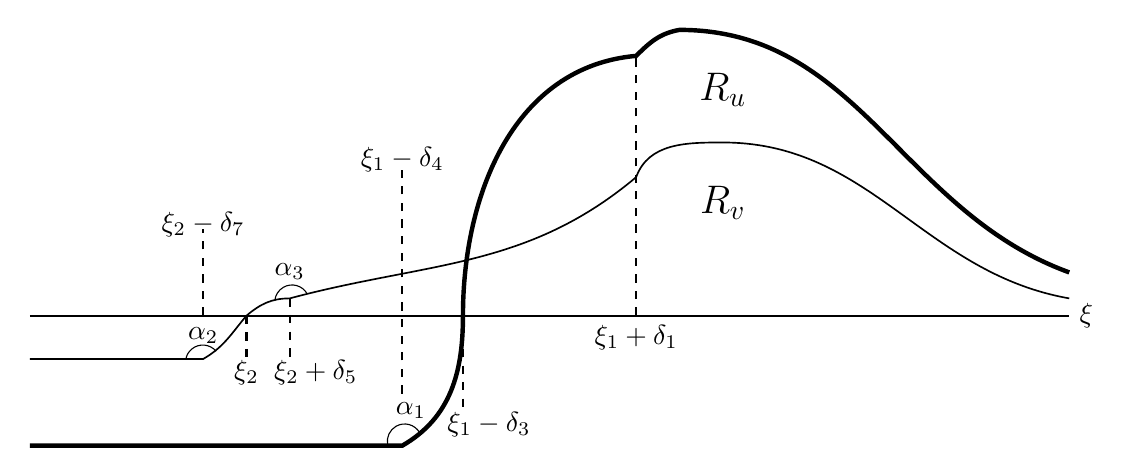
\begin{tikzpicture}[scale = 1.1]
\draw[thick](-6,0) -- (6,0) node[right] {$\xi$};
\draw [ultra thick] (-6,-1.5)--  (-1.7,-1.5)  to [out=30,in=270]   (-1,0)  to [out=90,in=185]  (1,3) to [out=45,in=190] (1.5,3.3) to [out=0,in=160] (6,0.5);
\draw [semithick] (-6, -0.5) -- (-4,-0.5) to [out=30, in=230] (-3.5,0)  to [out= 40, in=180] (-3,0.2) to [out=15, in=220] (1,1.6) to [out=70,in=180] (2,2)to [out=0,in=170] (6,0.2);
\node[below] at (1,0) {$\xi_{1}+\delta_1$};
%\node[below] at (0,-0.1) {$\xi_{\sigma}$};
\draw[dashed] [thick] (-3.5,0)-- (-3.5,-0.5);
\node[below] at (-3.5,-0.4) {$\xi_2$};
\draw[dashed] [thick] (-3,0.2)-- (-3,-0.5);
\node[below] at (-2.7,-0.4) {$\xi_2+\delta_5$};
\draw[dashed] [thick] (-4,0)-- (-4,1);
\node[above] at (-4,0.8) {$\xi_2-\delta_7$};
\draw[dashed] [thick] (1,0)-- (1,3);
\draw[dashed] [thick] (-1,0)-- (-1,-1.1);
\draw[dashed] [thick] (-1.7,-0.9)-- (-1.7,1.7);
\node[above] at (-1.7,1.55) {$\xi_1-\delta_4$};
%\node[below] at (-2.5,-0.2) {$\xi_2$};
%\draw[dashed] [thick] (-2.5,-0.3)-- (-2.5,0.3);
%\draw[dashed] [thick] (-2.5,-0.7)-- (-2.5,-1);
\node[below] at (-0.7,-1) {$\xi_1-\delta_3$};
\draw [thin] (-3.85,-0.41) arc [radius=0.2, start angle=40, end angle= 170];
\node[above] at (-4,-0.43) {$\alpha_2$};
%\draw [thin] (-2.3,0.355) arc [radius=0.2, start angle=30, end angle= 175];
%\node[above] at (-2.5,0.35) {$\alpha_4$};
\draw [thin] (-2.8,0.255) arc [radius=0.2, start angle=30, end angle= 175];
\node[above] at (-3,0.3) {$\alpha_3$};
\draw [thin] (-1.5,-1.35) arc [radius=0.2, start angle=30, end angle= 190];
\node[above] at (-1.6,-1.3) {$\alpha_1$};
%\draw [thin] (1.1,1.8) arc [radius=0.2, start angle=70, end angle= 220];
%\node[above] at (0.7,1.7) {$\alpha_1$};
%\draw [thin] (1.1,3.13) arc [radius=0.2, start angle=50, end angle= 180];
%\node[above] at (1,3.13) {$\alpha_2$};
%\node[above] at (2,1.5) {\Large{$v$}};
\node[above] at (2,2.3) {\Large{$R_u$}};
\node[above] at (2,1) {\Large{$R_v$}};
%\node[below] at (1,-2.3) {Figure \ref{Figure b<1}: $(R_u,R_v)$ for the case $0<b^*< 1$.};
\end{tikzpicture}
\caption{$(R_u,R_v)$ for the case $0<b^*< 1$.}\label{Figure b<1}
\end{center}
\end{figure}


We consider $(R_u,R_v)(\xi)$ defined  as (see Figure \ref{Figure b<1})
\begin{equation*}
(R_u,R_v)(\xi):=\begin{cases}
(\varepsilon_1\sigma(\xi) e^{-\lambda_u\xi},\eta_1(\xi-\xi_1) e^{-\lambda_u\xi}),&\ \ \mbox{for}\ \ \xi\ge\xi_1+\delta_1,\\
(\varepsilon_2\sin(\delta_2(\xi-\xi_1+\delta_3)),\eta_2e^{\lambda_{1}\xi}),&\ \ \mbox{for}\ \ \xi_1-\delta_4\le\xi\le\xi_{1}+\delta_1,\\
(-\delta_u,\eta_2e^{\lambda_{1}\xi}),&\ \ \mbox{for}\ \ \xi_2+\delta_5\le\xi\le\xi_1-\delta_4,\\
(-\delta_u,\eta_3\sin(\delta_6(\xi-\xi_2))),&\ \ \mbox{for}\ \ \xi_2-\delta_7\le\xi\le\xi_2+\delta_5,\\
(-\delta_u,-\delta_v),&\ \ \mbox{for}\ \ \xi\le\xi_2-\delta_7,
\end{cases}
\end{equation*}
where $\xi_1>M_0$ and $\xi_2<-M_0$ are fixed points, and $\lambda_{1}$ satisfies
\begin{equation}\label{condition on lambda 3}
d\lambda_1^2+2\sqrt{1-a}\,\lambda_1-r(2+b^*)>0\ \ {\rm and}\ \ \lambda_1>\frac{r(\hat v+1)}{2\sqrt{1-a}}.
\end{equation}
Here
$\varepsilon_{1,2}>0$, $\eta_{k=1,2,3}>0$, and $\delta_{i=1,\cdots,7}>0$ are chosen as same as that in Subsection 2.1.  Therefore, from \eqref{rho 2} and  $|R_u|,|R_v|\ll 1$, up to enlarging $M_0$, there exist $C_2>0$ and $C_3>0$ such that, for all $\xi\in(-\infty,\xi_2+\delta_5]$, it holds
\bea\label{xi 2 weak}
1-2U_*+R_u-aV_*-aR_v<-C_2<0,
\eea
and
\bea\label{xi 2 weak 2}
-(\hat v+\hat u\delta_0+C_3\rho)<1-2V_*-R_v-(b^*+\delta_0)U_*< C_3\rho.
\eea
Moreover, we set
\bea\label{delta u v}
\delta_u:=\varepsilon_2\sin(\delta_2(\delta_4-\delta_3))\quad\text{and}\quad \delta_v:=\eta_3\sin(\delta_6\delta_7),
\eea
which yield that $(R_u,R_v)(\xi)$ is continuous on $\mathbb{R}$.

Note that, for the construction in Subsection 2.1, we only set $|\delta_3-\delta_4|$  sufficiently small to obtain 
$$|R_u(\xi)|\ll|R_v(\xi_2+\delta_5)|\ \ \text{in}\ \ [\xi_2+\delta_5,\xi_1-\delta_3].$$
 However, for the weak competition case,
%and the critical case,
we will subtly set $\delta_u$ and $\delta_v$ to satisfy
\bea\label{delta u v 1}
\delta_v=\frac{b^*}{\sqrt{a}}\delta_u,
\eea
which can be done by modifying $|\delta_3-\delta_4|$ and $|\delta_7|$.

Now, we define
\beaa
(W_u,W_v)(\xi):=\Big(\min\{(U_*-R_u)(\xi),1\},\max\{(V_*+R_v)(\xi),0\}\Big),
\eeaa
and
%start to verify
show that $(W_u,W_v)$
%=(U_*-R_u,V_*+R_v)$
satisfies \eqref{tw super solution system}.
%for all $\xi\in\mathbb{R}$.
In fact, thanks to \eqref{rho 2} and \eqref{condition on lambda 3},
for $\xi\in[\xi_1-\delta_4,\infty)$, $N_3[W_u,W_v]\le 0$ and $N_4[W_u, W_v]\ge 0$ follow from the same argument as that in Subsection 2.1. Therefore, it suffices to  deal with $\xi\in (-\infty,\xi_1-\delta_4]$.
Next, we divide the discussion into three steps as follows.

\noindent{\bf{Step 1:}} We consider $\xi\in[\xi_2+\delta_5,\xi_1-\delta_4]$ with $\xi_2<-M_0$.
In this case, we have
\beaa
(R_u,R_v)(\xi)=(-\delta_u,\eta_2e^{\lambda_1\xi}),
\eeaa
where $\lambda_1$ satisfies \eqref{condition on lambda 3}, and $\delta_u$ is fixed as that in \eqref{delta u v}.
Note that, $\delta_u\to 0$ as $|\delta_3-\delta_4|\to 0$, and thus 
$$R'_u((\xi_1-\delta_{4})^+)>0=R'_u((\xi_1-\delta_{4})^-),\ i.e.\ \angle \alpha_1<180^{\circ}.$$

By some straightforward computations, since $R_v\ge 0$,
\bea\label{N3-step1 weak}
N_3[W_u,W_v]=\delta_u(1-2U_*-\delta_u-a(V_*+R_v))-aU_*R_v,
\eea
and $N_4[W_u,W_v]$ satisfies \eqref{N4-Step3}.

Note that, $\lambda_1$ and $\eta_2$ have already been determined by the construction on $\xi\in[\xi-\delta_4,\infty)$. Since $\frac{\rho}{2}\le U_*\le \hat u$ and $\hat v\le V_*\le 1$, by setting $|\delta_3-\delta_4|$ small enough such that
\bea\label{delta u 2}
\delta_u<\min\Big\{\frac{a\rho}{2\hat u},\frac{1}{4b^*}\Big\}\eta_2e^{\lambda_1(\xi_2+\delta_5)},
\eea
we have 
$$N_3[W_u,W_v]\le \delta_u(1-aV_*)-aU_*R_v\leq 0$$
 for $\xi\in[\xi_2+\delta_5,\xi_1-\delta_4]$.
Up to decreasing $\delta_0$ is necessary, $N_4[W_u,W_v]\geq 0$ follows immediately from \eqref{N4-Step3} and \eqref{delta u 2}. Thus, Step 1 is finished.

\medskip


\noindent{\bf{Step 2:}} We consider $\xi\in[\xi_2-\delta_7,\xi_2+\delta_5]$ with $\delta_7>0$ very small satisfying
\bea\label{cond delta 7 system}
\frac{2\sqrt{1-a}}{r\delta_7}-C_3\rho>2.
\eea
In this case, we have
\beaa
(R_u,R_v)(\xi)=\Big(-\delta_u,\eta_3\sin(\delta_6(\xi-\xi_2))\Big),
\eeaa
with
$\delta_6, \delta_7>0$ very small, and $\delta_5$ satisfies \eqref{cond delta 5}.
It follows from the same argument as Claim \ref{cl 5} that, there exist $\eta_3>0$ and small $\delta_6>0$
such that $R_v(\xi)$ is continuous at $\xi=\xi_2+\delta_5$ and $\angle\alpha_3<180^{\circ}$.

Note that $N_3[W_u,W_v]$ still satisfies \eqref{N3-step1 weak}.
Then, from \eqref{xi 2 weak} and  $R_v(\xi)>0$ for $\xi\in[\xi_2,\xi_2+\delta_5]$, we have $N_3[W_u,W_v]\le 0$  for $\xi\in[\xi_2,\xi_2+\delta_5]$. For $\xi\in[\xi_2-\delta_7,\xi_2]$, since $-\delta_v\le R_v\le 0$,
from \eqref{rho 2}, \eqref{delta u v 1}, and \eqref{N3-step1 weak}, we obtain that $N_3[W_u,W_v]\le 0$ up to increasing $M_0$ if necessary.

We next deal with the inequality of $N_4[W_u,W_v]$. For $\xi\in[\xi_2,\xi_2+\delta_5]$, by applying the same argument as Step 5 in Subsection 2.1, from \eqref{N4 inequality step 5}, \eqref{Rv-estimate2}, \eqref{condition on lambda 3}, and \eqref{xi 2 weak 2}, we have
\begin{equation*}
\begin{aligned}
N_4[W_u,W_v]\ge & rR_v\Big(1-2V_*-R_v-(b^*+\delta_0)U_*-\frac{d}{r}\delta_6^2\Big)+2\sqrt{1-a}\delta_6\eta_3\cos(\delta_6(\xi-\xi_2))\\
&+rV_*((b^*+\delta_0)R_u-\delta_0U_*)\\
\ge &r\Big(\frac{2\sqrt{1-a}}{r}\lambda_1-\hat v-\hat u\delta_0-C_3\rho-\frac{d}{r}\delta_6^2\Big)R_v(\xi_2+\delta_5)\\
&-r(\hat v+\rho)(b^*+\delta_0)\delta_u-r\delta_0\\
\ge & r(1-\hat u\delta_0-C_3\rho-\frac{d}{r}\delta_6^2)R_v(\xi_2+\delta_5)-r(\hat v+\rho)(b^*+\delta_0)\delta_u-r\delta_0
\end{aligned}
\end{equation*}
Recall that,
$\delta_u\ll R_v(\xi_2+\delta_5)$ up to decreasing $|\delta_3-\delta_4|$, and $\delta_6$ can be chosen sufficiently small such that $\frac{d}{r}\delta_6^2<\frac{1}{4}$. Then we have $N_4[W_u,W_v]\ge 0$ for $\xi\in[\xi_2,\xi_2+\delta_5]$, up to enlarging $M_0$ and decreasing $\delta_0$ if necessary.

For $\xi\in[\xi_2-\delta_7,\xi_2]$, since $R_v<0$ and $\xi_2<-M_0$, from \eqref{N4 inequality step 5}, \eqref{xi 2 weak 2}, and \eqref{cond delta 7 system}, we have
\begin{equation*}
\begin{aligned}
N_4[W_u,W_v]\ge & r(\frac{2\sqrt{1-a}}{r\delta_7}-C_3\rho)\delta_v-r(\hat v+\rho)(b^*+\delta_0)\delta_u-r\delta_0\hat u\\
\ge & 2r\delta_v-r(\hat v+\rho)(b^*+\delta_0)\delta_u-r\delta_0\hat u.
\end{aligned}
\end{equation*}
Then, from \eqref{delta u v 1}, we assert that $N_4[W_u,W_v]\ge 0$
up to decreasing $\delta_0$ if necessary.
Hence, the construction for Step 2 is finished.

\medskip

\noindent{\bf{Step 3:}} We consider $\xi\in(-\infty,\xi_2-\delta_7]$.
In this case, we have
\beaa
(R_u,R_v)(\xi)=(-\delta_u,-\delta_v).
\eeaa
Since $\delta_7\ll\frac{\pi}{2\delta_6}$, we see 
$$R'_v((\xi_2-\delta_7)^-)=0<R'_v((\xi_2-\delta_7)^+),\ i.e.,\ \angle\alpha_2<180^{\circ}.$$

By applying the same argument as Step 2 above, $N_3[W_u,W_v]\le 0$ for $\xi\in(-\infty,\xi_2-\delta_7]$. Therefore, it suffices to verify the inequality of $N_4[W_u,W_v]$.  By some straightforward computations, from \eqref{rho 2}, we have
\begin{equation*}
\begin{aligned}
N_4[W_u,W_v]= & -rV_*(b^*+\delta_0)\delta_u-r\delta_v\Big[1-2V_*+\delta_v-(b^*+\delta_0)(U_*+\delta_u)\Big]\\
\ge & -r(\hat v+\rho)(b^*+\delta_0)\delta_u-r\delta_v\Big[1-2\hat v+\delta_v-(b^*+\delta_0)(\hat u+\rho+\delta_u)\Big].
\end{aligned}
\end{equation*}
Then, from \eqref{delta u v 1} and $0<b^*<1$, we have $N_4[W_u,W_v]\ge 0$ up to enlarging $M_0$ and decreasing $\delta_0$ if necessary. The construction for Step 3 is complete.




\bigskip
\subsection{Proof of Theorem~\ref{th:threshold}}

\noindent

We first prove Proposition~\ref{Prop-supersol-system}.

\begin{proof}[Proof of Proposition~\ref{Prop-supersol-system}]
Combining the construction of $(R_u,R_v)$ in Subsection~\ref{sec:3-1} and Subsection~\ref{sec:3-2},
we are now equipped with a super-solution
\beaa
(W_u,W_v)=(\min\{U_*-R_u,1\},\max\{V_*+R_v,0\})
\eeaa
satisfying \eqref{tw super solution system}.
Moreover, at the points of discontinuity of $W'_u$ and $W'_v$,
the corresponding one-sided derivatives have the right sign.
Therefore, we complete the proof of Proposition~\ref{Prop-supersol-system}.
\end{proof}






We are now ready to prove Theorem~\ref{th:threshold}.

%%%%%%%%%%%%%%%%%%%%%%%%%%%%%%%%%%%%%%%%%%%%%%%%%%%%%%%%%%%%%%%%%%%%%%%%%%%%%%%%%%%%%%
\begin{proof}[Proof of Theorem~\ref{th:threshold}]
In view of Lemma~\ref{lm: existence b*}, it suffices to show that conditions (i) and (ii) are equivalent.
We now deal with ${\rm(i)}\Leftrightarrow {\rm(ii)}$. To prove ${\rm(i)}\Rightarrow{\rm(ii)}$, we use the contradiction argument and assume that (ii) is not true, by Lemma~\ref{lm: behavior around + infty} (ii), we see that $U_*$ satisfies \eqref{AS-U-infty-for-contradiction} and thus Proposition~\ref{Prop-supersol-system} is available.

To reach a contradiction, we consider the Cauchy problem
\begin{equation}\label{system2}
\left\{
\begin{aligned}
&\partial_tu=u_{xx}+u(1-u-av), & t>0,\ x\in\mathbb{R},\\
&\partial_tv=dv_{xx}+rv(1-v-(b^*+\delta_0)u), & t>0,\ x\in \mathbb{R},\\
&u(0,x)=u_0(x),\quad  v(0,x)\equiv1, & \ x\in \mathbb{R},
\end{aligned}
\right.
\end{equation}
where $u_0(x)$ %and $v_0(x)$ are
is compactly supported continuous function. Additionally we assume $\max_{x\in\mathbb{R}} |u_0(x)|<\frac{1-a}{1-ab^*}$ and $\delta_0>0$ is sufficiently small such that
$b^*+\delta_0\neq 1$ if $b^*<1$.
%\red{Then} the corresponding critical front $(c^*,U_*,V_*)$ satisfies \eqref{tw solution} with $b=b^*+\delta_0$ and \red{$c^{**}(b)=c^{**}(b^*+\delta_0)$}.
By the definition of $b^*$, we see that the minimal traveling wave speed $c^{*}_{LV}(b^*+\delta_0)$ corresponding to the system \eqref{tw solution weak} with $b=b^*+\delta_0$ satisfies $c^{*}_{LV}(b^*+\delta_0)>2\sqrt{1-a}$.
Then, according to results from \cite{Lewis Li Weinberger 1, Lewis Li Weinberger 2},
%Thus, from Theorem 1.4 of \cite{Wu Xiao Zhou},
the spreading speed of \eqref{system2} is
exactly $c^{*}_{LV}(b^*+\delta_0)$, strictly greater than $2\sqrt{1-a}$.

Let $(W_u, W_v)$ be constructed in Proposition~\ref{Prop-supersol-system}. Then, thanks to Proposition~\ref{Prop-supersol-system}, it is easy to see that
$(\bar{u},\underline{v})(t,x):=(W_u,W_v)(x-(2\sqrt{1-a})t-\eta)$, forms a super-solution for \eqref{system2} for all $t\ge 0$ and $x\in\mathbb{R}$, where $\eta\in\mathbb{R}$ is chosen large enough to have $\bar{u}(0,x)\geq u_0(x)$ and $\underline{v}(0,x)\leq v_0(x)$ for $x\in\mathbb{R}$.
By applying the comparison principle, we assert that the spreading speed of \eqref{system2} is smaller than or equal to $2\sqrt{1-a}$,
which reaches a contradiction.
%since $\sigma$ is arbitrarily small.
The proof of ${\rm(i)}\Rightarrow {\rm(ii)}$ is finished.

Next, we show ${\rm(ii)}\Rightarrow {\rm(i)}$. Note that for $b>b^*$, the speed is nonlinearly selected, which together with Lemma~\ref{lm: behavior around + infty} implies that (ii) cannot hold. Therefore, it suffices to show that (ii) cannot happen with
$b<b^*$. We assume by contradiction that that there exists $b^\dag\in(0,b^*)$ such that
\beaa
U_{b^\dag}(\xi)=B^\dag e^{-\lambda_u \xi}+o(e^{-\lambda_u \xi})\quad \mbox{as $\xi\to\infty$}
\eeaa
for some $B^\dag>0$.
In view of the asymptotic behavior of fronts at $\pm\infty$ given in the Appendix, we can define
\beaa
L^*:=\inf\{L\in\mathbb{R}|\, U_{*}(\xi-L)\geq U_{b^\dag}(\xi),\ V_{*}(\xi-L)\leq V_{b^\dag}(\xi),\ \forall \xi\in\mathbb{R}\}.
\eeaa
Note that,  we should divide the discussion into several cases: $b^*>1$ and $b^\dag>1,=1,\text{or}<1$; $b^*=1$ and $b^\dag=1,\text{or}<1$; $b^*<1$ and $b^\dag<1$. But to define $L^*$ we only need $0<b^\dag<b^*$.

Next, we will apply the sliding method  to reach a contradiction. By the continuity, we have 
$$U_{b^*}(\xi-L^*)\geq U_{b^\dag}(\xi)\ \ \text{and}\ \ 1-V_{b^*}(\xi-L^*)\geq 1-V_{b^\dag}(\xi)\ \ \text{for all}\ \ \xi\in\mathbb{R}.$$
 If there exists $\xi^*\in\mathbb{R}$ such that
$$U_{b^*}(\xi^*-L^*)= U_{b^\dag}(\xi^*)\ \ \text{or}\ \ 1-V_{b^*}(\xi^*-L^*)=1- V_{b^\dag}(\xi^*),$$
by the strong maximum principle, we have $(U_{b^*},V_{b^*})(\xi-L^*)= (U_{b^\dag},V_{b^\dag})(\xi)$ for all $\xi\in\mathbb{R}$,
which is impossible since they satisfy different equations. Consequently,
\bea\label{U*>U+}
U_{b^*}(\xi-L^*)> U_{b^\dag}(\xi),\quad V_{b^*}(\xi-L^*)< V_{b^\dag}(\xi)\quad \mbox{ for all $\xi\in\mathbb{R}$}.
\eea


Furthermore, we claim that the touch point cannot happen at $-\infty$.
\begin{claim}\label{claim 1 to proof th 1.5}
It holds
\beaa
\text{{\rm(I)}}\lim_{\xi\to-\infty}\frac{1-U_{b^*}(\xi-L^*)}{1-U_{b^\dag}(\xi)}<1\quad\text{and}\quad\text{{\rm(II)}}\lim_{\xi\to-\infty}\frac{V_{b^*}(\xi-L^*)}{V_{b^\dag}(\xi)}<1.
\eeaa
\end{claim}
\begin{proof}
Without loss of generality, we only deal with the case $1<b^\dag<b^*$. The others can be proved by the same argument.
Recall that $\mu^+_u(c^*)$ and $\mu^+_v(c^*)$ defined as that in Lemma \ref{lem:AS-infty:b>1}.
Let us denote for simplicity that
\beaa
\mu_u=\mu^+_u(c^*),\quad  \mu_{v,1}=\mu^+_v(c^*,b^*),\quad  \mu_{v,2}=\mu^+_v(c^*,b^\dag).
\eeaa
Note that $\mu_u$ is independent of $b$.
Clearly, it follows from the definition of $\mu_{v,i}$, $i=1,2$, that $\mu_{v,1}>\mu_{v,2}$.
Then (II) immediately follows from Lemma \ref{lem:AS-infty:b>1}.
%  and  since $V_{b^*}$ and $V_{b^\dag}$ have different decay rates.

Next, we deal with (I).
First, we consider the case $\mu_u\ge \mu_{v,2}$. Since $\mu_{v,1}>\mu_{v,2}$,
(I) follows immediately from Lemma~\ref{lem:AS-infty:b>1} since $1-U_{b^*}(\xi)$ decays faster than
$1-U_{b^\dag}(\xi)$ as $\xi\to-\infty$.

%For the cases $\mu_u\ge \mu_{v,1}>\mu_{v,2}$ and $\mu_{v,1}>\mu_u\ge \mu_{v,2}$, it follows immediately from Lemma \ref{lem:AS-infty:b>1} since $1-U_{b^*}$ and $1-U_{b^\dag}$ have different decay rates.
For the case $\mu_{v,2}>\mu_u$,
%by some straightforward computations, from $U$-equation there exist $C_1>0$ such that $1-U_{b^*}(\xi-L^*)=C_1V_{b^*}(\xi-L^*)$ and $1-U_{b^\dag}(\xi-L^*)=C_1V_{b^\dag}(\xi-L^*)$
we assume by the  contradiction that
$$\lim_{\xi\to-\infty}\frac{1-U_{b^*}(\xi-L^*)}{1-U_{b^\dag}(\xi)}=1.$$
Then from Lemma \ref{lem:AS-infty:b>1}, there exist $C_1,C_2>0$ satisfying $C_1=C_2e^{\mu_u L^*}$ such that 
$$1-U_{b^*}(\xi-L^*)\approx C_1e^{\mu_u\xi}\ \ \text{and}\ \ 1-U_{b^\dag}(\xi)\approx C_2e^{\mu_u\xi}\ \ \text{as}\ \ \xi\to-\infty.$$

%On the other hand,
To reach a contradiction,
we set
\beaa
U_1(\xi)=(1-U_{b^\dag}(\xi))-(1-U_{b^*}(\xi-L^*)), \quad V_1(\xi):= V_{b^\dag}(\xi)-V_{b^*}(\xi-L^*).
\eeaa
Then, by \eqref{U*>U+},
$U_1(\xi)>0$ and $V_1(\xi)>0$ for all $\xi\in\mathbb{R}$, Moreover, $U_1$ satisfies
\bea\label{U1-eq}
U_1''+c^* U_1'-U_1+aV_1+g_1+g_2=0,\quad \xi\in\mathbb{R}.
\eea
where
\beaa
&&g_1(\xi)=[2-U_{b^\dag}(\xi)-U_{b^*}(\xi-L^*)-aV_{b^*}(\xi-L^*)]U_1(\xi),\\
&&g_2(\xi)=-a(1-U_{b^\dag}(\xi))V_1(\xi).
\eeaa
It is clear that $g_1(\xi)=o(U_1(\xi))$ as $\xi\to-\infty$. Next, we show that $(aV_1+g_2)(\xi)$ also satisfies $(aV_1+g_2)(\xi)=o(U_1(\xi))$ as $\xi\to-\infty$.

By using 
%$C_1=C_2e^{\mu_u L^*}$, 
$1-U_{b^\dag}(\xi)\approx C_2e^{\mu_u\xi}$ and $V_1(\xi)\approx C_3e^{\mu_{v,2}\xi}$ (for some $C_3>0$) as $\xi\to-\infty$,
we assume by contradiction that $U_1(\xi)=\alpha(\xi)e^{(\mu_u+\mu_{v,2})\xi}$, with $\alpha(\xi)=O(1)$ or $o(1)$. By $(aV_1+g_2)(\xi)>0$ and the definitions of $\mu_u,\mu_{v,2}$, we obtain
\beaa
U_1''+c^* U_1'-U_1+aV_1+g_1(\xi)+g_2(\xi)>0\quad \mbox{for all large negative $\xi$,}
\eeaa
which contradicts \eqref{U1-eq}. Then, we can assert that $(aV_1+g_2)(\xi)=o(U_1(\xi))$ as $\xi\to-\infty$.

Therefore, by applying \cite[Chapter 3, Theorem 8.1]{CoddingtonLevison}, the asymptotic behavior of $U_1(\xi)$ at $\xi=-\infty$ satisfies $U_1(\xi)\approx e^{\mu_u \xi}$ which contradicts to $C_1=C_2e^{\mu_u L^*}$. The proof of Claim \ref{claim 1 to proof th 1.5} is complete.
\end{proof}


Now, we are  ready to prove that the touch point always happens on $U$-equation at $+\infty$.
\begin{claim}\label{claim 2 of proof of th 1.5}
It holds
\beaa
\lim_{\xi\to+\infty}\frac{U_{b^*}(\xi-L^*)}{U_{b^\dag}(\xi)}=1.
\eeaa
\end{claim}
\begin{proof}
Let $\lambda_v^-(c^*)<0$ be defined as in Lemma \ref{lm: behavior around + infty}. For the case $\lambda_v^-(c^*)\le -\sqrt{1-a}$,
we are going to prove
\bea\label{aaaaa}
\lim_{\xi\to+\infty}\frac{U_{b^*}(\xi-L^*)}{U_{b^\dag}(\xi)}>1\Longrightarrow \lim_{\xi\to+\infty}\frac{1-V_{b^*}(\xi-L^*)}{1-V_{b^\dag}(\xi)}>1.
\eea
%o do this, it is suffice to assume $U_{b^*}(\xi-L^*)=(1+\delta)U_{b^\dag}(\xi)$ with very small $\delta>0$. By some %straightforward computations and Lemma \ref{lm: behavior around + infty}, we have
We divide our discussion into three cases:
\begin{itemize}
    \item[(1)] if $\lambda_v^-(c^*)< -\sqrt{1-a}$, then by Lemma \ref{lm: behavior around + infty},
    we see that $U_b(\xi)$ and $1-V_b(\xi)$ have the same decay rate at $+\infty$ and there exists a positive constant $A_1$ such that
    \beaa
    \lim_{\xi\to+\infty}\frac{U_{b}(\xi)}{1-V_b(\xi)}=A_1.
    \eeaa
    Therefore, one has
    \beaa
     \lim_{\xi\to+\infty}\frac{1-V_{b^*}(\xi-L^*)}{1-V_{b^\dag}(\xi)}&=&
     \lim_{\xi\to+\infty}\Big[\frac{1-V_{b^*}(\xi-L^*)}{U_{b^*}(\xi-L^*)}\frac{U_{b^*}(\xi-L^*)}{U_{b^\dag}(\xi)}
     \frac{U_{b^\dag}(\xi)}{1-V_{b^\dag}(\xi)}\Big]\\
     &=&\frac{1}{A_1}\Big(\lim_{\xi\to+\infty}\frac{U_{b^*}(\xi-L^*)}{U_{b^\dag}(\xi)}\Big)A_1>1.
    \eeaa
    Hence \eqref{aaaaa} holds.

   %$ $$1-V_{b}(\xi-L^*)=\frac{rb}{(2-d)(1-a)+r}U_{b}(\xi-L^*);$$
    \item[(2)] if $\lambda_v^-(c^*)= -\sqrt{1-a}$, then by Lemma \ref{lm: behavior around + infty}, there exists a positive constant $A_2$ such that
    \beaa
    \lim_{\xi\to+\infty}\frac{\xi U_{b}(\xi)}{1-V_b(\xi)}=A_2.
    \eeaa
     Therefore, one has
    \beaa
     \lim_{\xi\to+\infty}\frac{1-V_{b^*}(\xi-L^*)}{1-V_{b^\dag}(\xi)}&=&
     \lim_{\xi\to+\infty}\Big[\frac{1-V_{b^*}(\xi-L^*)}{\xi U_{b^*}(\xi-L^*)}\frac{ U_{b^*}(\xi-L^*)}{U_{b^\dag}(\xi)}
     \frac{\xi U_{b^\dag}(\xi)}{1-V_{b^\dag}(\xi)}\Big]\\
     &=&\frac{1}{A_2}\Big(\lim_{\xi\to+\infty}\frac{U_{b^*}(\xi-L^*)}{U_{b^\dag}(\xi)}\Big)A_2>1,
    \eeaa
    which yields \eqref{aaaaa}.
    %$$1-V_{b}(\xi-L^*)=\frac{rb\xi}{2\sqrt{1-a}(d-1)}U_{b}(\xi-L^*).$$

    \item[(3)] if $\lambda_v^-(c^*)> -\sqrt{1-a}$, we assume by contradiction that
\bea\label{case-iii-lim}
\lim_{\xi\to+\infty}\frac{1-V_{b^*}(\xi-L^*)}{1-V_{b^\dag}(\xi)}=1.
\eea
Then from Lemma \ref{lm: behavior around + infty} and \eqref{case-iii-lim}, there exist $C_1,C_2>0$ satisfying $C_1=C_2e^{\lambda_v^-(c^*) L^*}$ such that 
$$1-V_{b^*}(\xi-L^*)\approx C_1e^{\lambda_v^-(c^*)\xi}\ \ \text{and}\ \ 1-V_{b^\dag}(\xi)\approx C_2e^{\lambda_v^-(c^*)\xi}.$$
To reach a contradiction, similar to the proof of Claim~\ref{claim 1 to proof th 1.5}, we set
\beaa
U_1(\xi):=U_{b^*}(\xi-L^*)-U_{b^\dag}(\xi), \quad V_1(\xi):= (1-V_{b^*}(\xi))-(1-V_{b^\dag}(\xi-L^*)).
\eeaa
Considering the equation satisfied by the positive function $V_1$:
\beaa
cV_1'+dV_1''-rV_1+rbU_1+h_1(\xi)+h_2(\xi)=0,\quad \xi\in\mathbb{R},
\eeaa
where
\beaa
&&h_1(\xi)=r[2-V_{b^*}(\xi)-V_{b^\dag}(\xi-L^*)]V_1(\xi),\\
&&h_2(\xi)=-r b(1-V_{b^\dag}(\xi-L^*))U_1(\xi).
\eeaa
Using a similar argument as in Claim \ref{claim 1 to proof th 1.5}, we can reach a contradiction, and thus \eqref{aaaaa} holds.
\end{itemize}

%Therefore, by $b^{\dag}<b^*$, \eqref{aaaaa} is proved.


%For the case $\lambda_v^-(c^*)> -\sqrt{1-a}$,
%we are going to prove
%$$\lim_{\xi\to+\infty}\frac{1-V_{b^*}(\xi-L^*)}{1-V_{b^\dag}(\xi)}>1.$$
%We assume by contradiction that
%$$\lim_{\xi\to+\infty}\frac{1-V_{b^*}(\xi-L^*)}{1-V_{b^\dag}(\xi)}=1.$$
%Then from Lemma \ref{lm: behavior around + infty}, there exist $C_1,C_2>0$ satisfying $C_1=C_2e^{\lambda_v^-(c^*) L^*}$ such that $1-V_{b^*}(\xi-L^*)\approx C_1e^{\lambda_v^-(c^*)\xi}$ and $1-V_{b^\dag}(\xi)\approx C_2e^{\lambda_v^-(c^*)\xi}$.
%On the other hand, we set $V_1(\xi)=(1-V_{b^*}(\xi))-(1-V_{b^\dag}(\xi-L^*))$. Then $V_1(\xi)$ is a positive solution of the following linear equation
%\beaa
%dV_1''+c^* V_1'-rV_1\Big(1-\frac{b^*(U_{b^*}(\xi-L^*)-b^\dag U_{b^\dag}(\xi))}{V_1}+o(1)\Big) =0.
%\eeaa
%In particular, we have
%$$\frac{b^*(U_{b^*}(\xi-L^*)-b^\dag U_{b^\dag}(\xi))}{V_1}=o(1).$$
%Otherwise, there exists $C_3>0$ such that $V_1(\xi)\approx C_3e^{-\sqrt{1-a}\xi}$ which implies
%\beaa
%dV_1''+c^* V_1'-rV_1\Big(1-\frac{b^*(U_{b^*}(\xi-L^*)-b^\dag U_{b^\dag}(\xi))}{V_1}+o(1)\Big) >0
%\eeaa
%since $\lambda_v^-(c^*)> -\sqrt{1-a}$.
%Then, applying \cite[Chapter 3, Theorem 8.1]{CoddingtonLevison} and similar argument in Claim \ref{claim 1 to proof th 1.5},
%we reach a contradiction.

As a result, if Claim \ref{claim 2 of proof of th 1.5} is not true,
from Claim \ref{claim 1 to proof th 1.5} and \eqref{aaaaa}, %we can use standard argument to find
it is easy to see that there exists
$\varepsilon>0$ sufficiently small such that
$W_{s^*}(\xi-(L^*+\varepsilon))> W_{s_0}(\xi)$ for $\xi\in\mathbb{R}$,
which contradicts the definition of $L^*$. Therefore,
the proof of Claim \ref{claim 2 of proof of th 1.5} is finished.
\end{proof}


Now, we are ready to finish the proof of ${\rm(ii)}\Rightarrow {\rm(i)}$
%Theorem \ref{th:threshold}
by the help of Claim \ref{claim 1 to proof th 1.5} and  Claim  \ref{claim 2 of proof of th 1.5}.
For this, we set
\beaa
U_2(\xi):=U_{b^*}(\xi-L^*)-U_{b^\dag}(\xi), \quad V_2(\xi):= (1-V_{b^*}(\xi))-(1-V_{b^\dag}(\xi-L^*)).
\eeaa
Then we focus on the equation satisfied by $U_2$ and
use a similar argument as in Claim \ref{claim 1 to proof th 1.5}, we can again reach a contradiction.
%We set $U_2(\xi)=U_{b^*}(\xi-L^*)-U_{b^{\dag}}(\xi)$. Then $U_2(\xi)$ satisfies
%\beaa
%U_2''+c^* U_2'+U_2\Big(1-a+\frac{a(U_{b^*}(1-V_{b^*})(\xi-L^*)- U_{b^\dag}(1-V_{b^\dag})(\xi))}{U_2}+o(1)\Big)=0.
%\eeaa
%In particular, we have
%$$\frac{a(U_{b^*}(1-V_{b^*})(\xi-L^*)- U_{b^\dag}(1-V_{b^\dag})(\xi))}{U_2}=o(1).$$
%Otherwise, from the asymptotic behavior of $U_2(+\infty)$ and the fact $U_{b^*}(1-V_{b^*})(\xi-L^*)- U_{b^\dag}(1-V_{b^\dag})%(\xi)>0$, we have
%\beaa
%U_2''+c^* U_2'+U_2\Big(1-a+\frac{a(U_{b^*}(1-V_{b^*})(\xi-L^*)- U_{b^\dag}(1-V_{b^\dag})(\xi))}{U_2}+o(1)\Big)>0.
%\eeaa
%Then, applying \cite[Chapter 3, Theorem 8.1]{CoddingtonLevison},
%%{Maybe we need more details or references here}
%the asymptotic behavior of $U_2(\xi)$ at $\xi=+\infty$ satisfies
%\beaa
%U_2(\xi)=(C_1\xi+C_2)e^{-\beta \xi}+o(e^{-\beta\xi})\quad \mbox{as $\xi\to\infty$},
%\eeaa
%where  $C_1\geq0$, and $C_2>0$ if $C_1=0$. From \eqref{bbbb} and the asymptotic behavior of $U_{b^*}$, we see that $C_1=0$.
%Thus, it holds that $C_2>0$. However, Claim \ref{claim 2 of proof of th 1.5} implies $B_\dag=Be^{\sqrt{1-a} L^*}$ implies that %$C_2=0$, which reaches a contradiction.
Consequently, we obtain
${\rm(ii)}\Rightarrow {\rm(i)}$.  This completes the proof of Theorem \ref{th:threshold}.
%Finally, note that ${\rm(ii)}\Leftrightarrow {\rm(iii)}$ follows from Lemma~\ref{lm: behavior around + infty} and Proposition~\ref{prop: implicit cond}.
\end{proof}


\bigskip

%%%%%%%%%%%%%%%%%%%%%%%%%%%%%%%%%%%%%%%%%%%%%%%%%%%%%%%%%%%%%%%%

\section{Sufficient condition (II) for the speed nonlinear selection}


Regarding the second sufficient condition for the speed nonlinear selection to \eqref{system}, 
we fix $r,d>0$, \red{$b>1$} and 
focus on the degenerate case $a=1$. 
We will show the existence of the \red{minimal speed} of traveling wave solutions for this degenerate case and discuss the continuity of the spreading speed on the parameter $a$. 
Here, the spreading speed is always defined by the solution starting from the initial datum satisfying \eqref{initial datum}. 
As a result, we find that when $a\in(0,1)$ is sufficiently close to the critical value $a=1$, the spreading speed becomes nonlinearly selected.

%In this section, 
We shall first discuss the continuity of spreading speed of \eqref{system} on both competition coefficients $a>0$ and $b>1$. 
For any given $b>1$, the system \eqref{system} is of bistable type when $a>1$, which admits a unique traveling wave solution and a unique traveling wave speed $\hat c_{LV}(a)$ satisfying \eqref{tw solution weak} (see \cite{Kan-On}). Moreover, it has been proved in \cite{Carrere,Peng Wu Zhou} that the spreading speed coincides with the speed of bistable fronts; namely, $c^{**}_{LV}(a)=\hat c_{LV}(a)$ for all $a>1$.
On the other hand, for any given $b>1$,
the system \eqref{system} with $a\in(0,1)$ is of monostable type which admits the minimal traveling wave speed $c^*_{LV}(a)$ satisfying \eqref{tw solution weak} (see \cite{Kan-on1997}). Furthermore, it has been proved in \cite{Lewis Li Weinberger 2} that $c^*_{LV}(a)=c^{**}_{LV}(a)$ for all $a\in(0,1)$. For the degenerate case $a=1$, the relation between the propagation speed and the minimal traveling speed has not been studied yet. 



To emphasize the dependence on both $a$ and $b$, we denote the spreading speed by $c^{**}_{LV}(a,b)$.
It is well known from \cite{Lewis Li Weinberger 2} for $0<a<1$ and $b>1$,
and  \cite{Carrere, Peng Wu Zhou} for $a,b>1$ that
\bea\label{spreading speed}
c^{**}_{LV}(a,b)=\begin{cases}
c^{*}_{LV}(a,b) &\quad \mbox{ if $0<a<1$ and  $b>1$;}\\
\hat{c}_{LV}(a,b) &\quad \mbox{ if $a>1$ and $b>1$},
\end{cases}
\eea
where $c^{*}_{LV}(a,b)$ denotes the minimal traveling wave speed; while 
$\hat{c}_{LV}(a,b)$ denotes the unique wave speed of bistable traveling waves.   


%Since the degeneracy only happens in the case $a=1$ or $b=1$. Thus, by apply the standard continuity argument, 

It is well known that $c^{**}_{LV}(a,b)$ is continuous on the following region
\beaa
\{(a,b)|\, 0<a<1,\ b>1\}\cup \{(a,b)|\, a>1,\ b>1\}.
\eeaa
%four square regions
%$$(1)\ 0<a,\ b<1;\ (2)\ 0<a<1<b;\ (3)\ 0<b<1<a;\ (4)\ a,\ b>1.$$
%and four intervals
%$$(1)\ a=1,\ 0<b<1;\ (2)\ a=1,\ b>1;\ (3)\ b=1,\ 0<a<1;\ (4)\ b=1,\ a>1.$$
%Furthermore, from the discussion in Proposition \ref{prop:existence-appendix}, we can conclude that $c^{**}_{LV}(a,b)$ is also continuous on $\{0<a<1,\ b=1\}$.
%two strip regions.
%$$(1)\ 0<a<1,\ b>0;\ (2)\ 0<b<1,\ a>0.$$
Therefore, to complete the continuity of $c^{**}_{LV}(a,b)$, it is sufficient to fix $b>1$ and prove $c^{**}_{LV}(a)$ is continuous at $a=1$. 
%The case $a>1$ and $b=1$ can be done by the same approach.

Notice that the propagation phenomenon of the critical case $a=b=1$ has been well studied in \cite{Alfaro Xiao}. Since the degeneracy on both $a=1$ and $b=1$, the propagation property of the solution does not depend on $a$ and $b$, but on the value of $dr$. As a result, it is meaningless to consider the continuity on $a=b=1$, and we exclude it from our discussion. 
Our main result reads as follows:


\begin{theorem}\label{th: continuity of the spread speed}
Let $r,d>0$ and $b>1$ in \eqref{system} be fixed. Then the following hold:
\begin{itemize}
    \item[(i)]  Define 
    \bea\label{A}
    A:=\{\tilde{c}\geq 0|\, \mbox{\eqref{tw solution weak} with $a=1$ has a monotone solution with $c=\tilde{c}$}\}.
    \eea
    Then the minimal speed of traveling wave solutions of \eqref{tw solution weak} with $a=1$ exists and is positive. Namely,
    $c^{*}_{LV}(1):=\min A$ is well-defined and is positive;
    \item[(ii)] The spreading speed of \eqref{system} with $a=1$ coincides with the minimal wave speed. Namely, $c^{**}_{LV}(1):=c^{*}_{LV}(1)>0$. Furthermore, 
    the spreading speed $c^{**}_{LV}(a)$ of \eqref{system} is continuous for all $a\in(0,\infty)$.
\end{itemize}
\end{theorem}


Then, by using the continuity argument, it follows immediately from Theorem \ref{th: continuity of the spread speed} that the propagation speed becomes nonlinear selection as $a\to 1$ from below.
\begin{theorem}\label{th: sufficient condition 2}
Let $r,d>0$ and $b>1$ in \eqref{system} be fixed. Then there exists a small $\varepsilon>0$ such that if $a\in (1-\varepsilon,1)$, then 
the spreading speed $c^{**}_{LV}(a)$ of \eqref{system} is nonlinearly selected.
\end{theorem}

Theorem~\ref{th: sufficient condition 2} generalizes the result given in \cite{HuangHan2011}.

% described as follows:

% \begin{proposition}[Theorem 4.1 of \cite{HuangHan2011}]
% Let $d =r$ and $b>1$ be fixed.
% Then there exists $\epsilon>0$ such that for all $a\in(1-\epsilon,1)$, the spreading speed $c^{**}_{LV}(a)$ of \eqref{system} is nonlinearly selected.
% \end{proposition}



\subsection{Existence of traveling waves in the case $a=1$}
We will first show the existence of traveling waves for the degenerate case $a=1$ and $b> 1$ by the approximation argument. 
%We denote 
By simple comparison, $c^*_{LV}(a)$ is nonincreasing for $a\in(0,1)$.
Therefore,
\bea\label{c-}
c_-:=\lim_{a\to 1^-} c^*_{LV}(a)\in[0,2)
\eea
is well-defined. 
%by $c^*_{LV}(a)$ to emphasize the dependence of $a\in (0,1]$.
\begin{proposition}\label{prop:existence-tw}
    Let $r,d>0$ and $b>1$ be given.  For any 
        $c\geq c_-$, %\liminf_{a\to 1^-} c^*_{LV}(a):=c_-, 
     there exists a monotone solution $(c,U,V)$ satisfies \eqref{tw solution weak} with $a=1$. %In other words, the minimal traveling wave speed satisfies $c^*_{LV}(1)\leq  c_-$
\end{proposition}
\begin{proof}
First, note that $c^*_{LV}(a)$ is nonincreasing for $a\in(0,1)$. Hence,
for each $c>c_-$, there exists a sequence $(c, U_n, V_n)$ such that $(U_n, V_n)$ is a monotone solution to \eqref{tw solution weak} with $a=a_n\in(0,1)$ and speed $c$.
Using the same argument as that in {\bf Claim A.2} in the Appendix, we can conclude that 
for each $c>c_-$, the system \eqref{tw solution weak} has a monotone solution with $a=1$ and speed $c$. Furthermore, by standard approximation argument, we can fix $a=1$ and take $c_n\downarrow c_-$
such that the system \eqref{tw solution weak} also admits a monotone solution with $a=1$ and speed $c=c_-$. This completes the proof.

    %Let $ c\geq \liminf_{a\to 1^-} c^*_{LV}(a)$ and take a sequence $a_n<1$ such that $a_n\to 1$ and 
%     \begin{equation*}
%         \lim_{n\to +\infty}  c^*_{LV}(a_n)\leq c.
%     \end{equation*}
%     Then by the well-known existence result from \cite{Kan-on1997}, there exists a sequence $(c_n, U_n, V_n)$ with $|c_n-c|\leq \frac{1}{n}$, such that $(U_n, V_n)$ is a monotone solution to \eqref{tw solution} with $a=a_n$ and $c=c_n$, in the sense that $U_n(\xi)$ is decreasing and $V_n(\xi)$ is increasing. Up to a shift in space we impose the following normalization on $V_n(\xi)$:
%     \begin{equation}\label{eq:normalization-tw-kanon}
%         V_n(0)=\frac{1}{2}.
%     \end{equation}
%     Then, it follows from the Arzel\`a-Ascoli Theorem that there exists a subsequence  locally uniformly converging to a limit $(U(\xi), V(\xi))$. Clearly $U(\xi)$ and $V(\xi)$ solve \eqref{tw solution} with speed $c$ and $a=1$. Moreover, since the limit is locally uniform and $U_n(\xi)$ is decreasing and $V_n(\xi)$ is increasing, then the limit $U(\xi)$ is decreasing (respectively: $V(\xi)$ is increasing). Finally it follows from the normalization \eqref{eq:normalization-tw-kanon} that
%     \begin{equation*}
%         V(0)=\frac{1}{2}.
%     \end{equation*}
%     Suppose by contradiction that $U(\xi)\equiv 0$. Then $V(\xi)$ is a monotone solution to 
%     \begin{equation}\label{eq:KPP-TW}
%         -cV'(\xi)-dV''(\xi)=rV(\xi)(1-V(\xi)), 
%     \end{equation}
%     and since it is increasing it has to connect $0$ near $-\infty$ to $1$ near $+\infty$. However multiplying \eqref{eq:KPP-TW} by $V'(\xi)$ and integrating, we get 
% \begin{equation*}
% -c\int_{\mathbb R}V'(\xi)^2 d\xi - \left[\frac{d}{2}V'(\xi)^2\right]_{-\infty}^{+\infty} = r\left[\frac{1}{2}V(\xi)^2 - \frac{1}{3}V(\xi)^3\right]_{-\infty}^{+\infty}=\frac{r}{6}, 
% \end{equation*}
% which leads to 
% \begin{equation*}
% c\int_{\mathbb R} U'(x)^2dx= -\frac{r}{6}, 
% \end{equation*}
%     which is clearly a contradiction since $c\geq 0$. We conclude that $U(x)$ is not identically $0$, and, since it is decreasing, it connects $1$ near $-\infty$ to $0$ near $+\infty$. Similarly $V(x)$ connects $0$ near $-\infty$ to $1$ near $+\infty$. Proposition \ref{prop:existence-tw} is proved.
\end{proof}

We next show that the minimal wave speed exists for $a=1$ and $b>1$.
The following proposition will show 
that any traveling wave speed for $a = 1$ and $b > 1$ must be strictly positive.

\begin{proposition}\label{prop: minimal tw speed c>0}
    %Assume system \eqref{system} with $a=1$ and $b>1$ admits a traveling wave solution 
Let $(c,U,V)$ satisfy \eqref{tw solution weak} with $a=1$ and $b>1$. Then $c>0$.
    %we have $c>0$.
\end{proposition}
\begin{proof} 
To do this, we assume $c\le 0$, then get the contradiction by some basic properties of traveling wave solutions. We first consider the case $d\le 1$.
We rewrite \eqref{tw solution weak} as 
\begin{equation*}
        \left\{
            \begin{aligned}
                &U''+cU'+U(1-U-V)=0,\\
                &V''+\frac{c}{d}V'+\frac{r}{d}V(1-V-bU)=0,\\
                &(U,V)(-\infty)=(1,0),\quad (U,V)(+\infty)=(0,1),\\
                &U'<0,\quad V'>0,\quad \xi\in\mathbb{R},
            \end{aligned}
            \right.
    \end{equation*}
and add the both sides of $U$-equation and $V$-equation to get
\begin{equation}\label{eq of U+V}
(U+V)''+c(U+V)'+c(\frac{1}{d}-1)V'+(U+\frac{r}{d}V)(1-U-V)+\frac{r}{d}(1-b)UV=0.
\end{equation}
%\begin{claim}\label{cl: U+V<1}
%        $U+V\le 1$ for all $z\in\mathbb{R}$, and $U+V<1$ for all $-\infty<\xi<+\infty$. 
%    \end{claim}
%\begin{proof}
We claim that 
\bea\label{U+V<1}
U(\xi)+V(\xi)<1 \quad \mbox{for all $-\infty<\xi<+\infty$}
\eea
If not, from the boundary conditions, we can find a local maximum point $\xi_0$ such that 
$$(U+V)(\xi_0)\geq 1,\ (U+V)'(\xi_0)=0,\ \ \text{and}\ \ (U+V)''(\xi_0)\leq0.$$
Then, since $c\leq 0$, $d\le 1$, $V'>0$, and $b>1$, the left hand of \eqref{eq of U+V} at $\xi=\xi_0$ is strictly negative. Therefore, we get the contradiction, and \eqref{U+V<1} holds.
 %$U+V\le 1$ for all $\xi\in\mathbb{R}$. 

%Now, by integrating the both sides of $U$-equation from $-\infty$ to $+\infty$, since Claim \ref{cl: U+V<1} the left hand becomes strictly negative unless $c=0$ and $U+V\equiv 1$ for all $\xi\in\mathbb{R}$. However, it is easy to prove from $V$-equation that $c=0$ and $U+V\equiv 1$ can not hold simultaneously.

To deal with the case $d> 1$, we rewrite \eqref{tw solution weak} as 
\begin{equation*}
        \left\{
            \begin{aligned}
                &bU''+cbU'+bU(1-bU-V)+b(b-1)U^2=0,\\
                &V''+\frac{c}{d}V'+\frac{r}{d}V(1-V-bU)=0,\\
                 &(U,V)(-\infty)=(1,0),\quad (U,V)(+\infty)=(0,1),\\
                &U'<0,\quad V'>0,\quad \xi\in\mathbb{R},
            \end{aligned}
            \right.
    \end{equation*}
and add the both sides of $U$-equation and $V$-equation to get
\begin{equation}\label{eq of bU+V}
(bU+V)''+c(bU+V)'+c(\frac{1}{d}-1)V'+(bU+\frac{r}{d}V)(1-bU-V)+b(1-b)U^2=0.
\end{equation}
    % \begin{claim}\label{cl: bU+V>1}
    %     $bU+V\ge 1$ for all $z\in\mathbb{R}$, and $bU+V>1$ for all $-\infty<\xi<+\infty$. 
    % \end{claim}
    % \begin{proof}
Next, we will show 
\bea\label{bU+V>1}
bU(\xi)+V(\xi)> 1 \quad \mbox{for all $-\infty<\xi<+\infty$}
\eea
%$bU+V\ge 1$ for all $\xi\in\mathbb{R}$. 
If not, we can find a local minimum point $\xi_0$ such that 
$$(bU+V)(\xi_0)\leq 1,\ (bU+V)'(\xi_0)=0,\ \ \text{and}\ \ (bU+V)''(\xi_0)\geq 0.$$
Then, since $c\leq 0$, $d> 1$, $V'>0$, and $b>1$, the left hand of \eqref{eq of bU+V} at $\xi=\xi_0$ is strictly positive. Therefore, we get the contradiction, and \eqref{bU+V>1} holds. This completes the proof.
%$bU+V\ge 1$ for all $\xi\in\mathbb{R}$. 
% Now, by integrating the both sides of $V$-equation from $-\infty$ to $+\infty$, since Claim \ref{cl: bU+V>1} the left hand becomes strictly negative unless $c=0$ and $bU+V\equiv 1$ for all $\xi\in\mathbb{R}$. 
% However, it is easy to get contradiction from $U$-equation, and we claim $c=0$ and $bU+V\equiv 1$ can not hold simultaneously.
\end{proof}


In view of Proposition~\ref{prop:existence-tw} 
and Proposition~\ref{prop: minimal tw speed c>0}, we have

\begin{corollary}\label{cor:c_lv(1)}
Let $r,d>0$ and $b>1$ be given. Then the minimal speed of traveling wave solutions
of \eqref{tw solution weak} with $a=1$ exists and is positive. That is, 
\beaa
c^{*}_{LV}(1):=\min A\in(0, c^-].
\eeaa
is well-defined.
where $A$ is defined in \eqref{A}.
\end{corollary}
\begin{proof}
By Proposition~\ref{prop:existence-tw} and Proposition~\ref{prop: minimal tw speed c>0},
we see that the set $A$ is nonempty and has a lower bound zero. Therefore, 
$\inf A$ is well-defined. Moreover, by standard approximation argument, 
we can conclude that \eqref{tw solution weak} also has a monotone solution with $c=\inf A$ and $a=1$, which implies that $c^{*}_{LV}(1):=\min A\geq0$ is well-defined. 
In addition, in view of Proposition~\ref{prop:existence-tw}, we have $c^{*}_{LV}(1)\leq c_-$. By Proposition~\ref{prop: minimal tw speed c>0}, we have 
$c^{*}_{LV}(1)>0$. This completes the proof.
\end{proof}



\subsection{Continuity of the spreading speed}

Now, we fix $b>1$, $r,d>0$, and establish the continuity of the spreading speed of \eqref{system} on $a\in(0,\infty)$. 
%Here, the spreading speed is always defined by the solution starting from the initial datum satisfying \eqref{initial datum}.  
% For any given $a\in(1,\infty)$, the system \eqref{system} is of bistable type which admits a unique traveling wave solution and traveling wave speed $\hat c_{LV}(a)$ satisfying \eqref{tw solution}. Moreover, it has been proved in \cite{Carrere,Peng Wu Zhou} that $\hat c_{LV}(a)=c^{**}_{LV}(a)$ for all $a\in(1,\infty)$.
% On the other hand, for any given $a\in(0,1)$, the system \eqref{system} is of monostable type which admits a minimal traveling wave speed $c^*_{LV}(a)$ satisfying \eqref{tw solution}. Moreover, it has been proved in \cite{Girardin Lam} that $c^*_{LV}(a)=c^{**}_{LV}(a)$ for all $a\in(0,1)$. For the degenerate case $a=1$, the relation between the propagation speed and the minimal traveling speed has not been studied yet. 
% The super and sub-solution approach cannot be used since traveling wave solutions  probably converge to the state $(U,V)=(0,1)$ algebraically fast (see Proposition \ref{prop:asym-invaded} and \ref{prop decay rate a=1}). More precisely, under some certain conditions, the decay rate of the minimal traveling wave solution is not of exponential order, but polynomial order.
%We first 
It suffices to discuss the continuity on %the minimal traveling wave speed 
the spreading speed $c^{**}_{LV}(a)$ %$c^*_{LV}$ 
at $a=1$ on both direction $a\to 1^+$ and $a\to 1^-$. 
%Notice 
Recall from \cite{Kan-On} that, for $a>1$, 
the system \eqref{system} admits a unique traveling wave solution with unique speed $\hat{c}_{LV}(a)\in[-2\sqrt{rd},2]$. Moreover, 
$\hat{c}_{LV}(a)$ is strictly decreasing for $a>1$.
Therefore, we can  
%Here, we treat this unique speed as the minimal traveling wave speed for $a>1$.
define 
\bea\label{c+}
c_+:=\lim_{a\to 1^+}\hat c_{LV}(a).
\eea

% Our main result in this subsection read as follows:
% \begin{theorem}\label{th: continuity of the minimal speed}
% Let $r,d>0$ and $b>1$ in \eqref{system} be fixed. Then the minimal traveling wave speed $c^{*}_{LV}(a)$ of \eqref{system} is continuous for all $a\in(0,\infty)$. Moreover, we have $c^{*}_{LV}(1)=c^{**}_{LV}>0$.
% \end{theorem}



%Note that, 
The relation between $c^*_{LV}(1)$ and $c_-$ follows %immediately from %Proposition \ref{prop:existence-tw}, 
from Corollary~\ref{cor:c_lv(1)},
i.e. $c^*_{LV}(1)\le c_-$. To prove the continuity of %$c^*_{LV}(a)$, 
$c^{**}_{LV}(a)$,
we also need to figure out the relation between $c^*_{LV}(1)$ and $c_+$.

\begin{lemma}\label{prop: c**<hat c}
Let $b>1$ be given. Then we have $c^*_{LV}(1)\ge c_+$.
\end{lemma}
\begin{proof}
This Lemma follows immediately from some comparison argument. Assume by contradiction that $c^*_{LV}(1)< c_+$. Then, there exists $\delta_0$ small enough such that the traveling wave speed of \eqref{system} with $a=1+\delta_0$ satisfying $\hat c_{LV}(1+\delta_0)\in(c^*_{LV}(1),c_{+})$. Denote $(c^*_{LV}(1),\hat U,\hat V)$ as the traveling wave solution of \eqref{system} with $a=1$. It is easy to check that 
$$(\hat U(x-c^*_{LV}(1)t-x_0),\hat V(x-c^*_{LV}(1)t)-x_0)$$ is a super-solution of
\begin{equation}\label{system a=1+delta}
    \left\{\begin{aligned}\relax
    & u_t=u_{xx}+u(1-u-(1+\delta_0)v) \\ 
        & v_t=dv_{xx}+rv(1-bu-v). 
    \end{aligned}\right.
\end{equation}
It has been proved in Theorem 3 of \cite{Peng Wu Zhou} that, the spreading speed of \eqref{system a=1+delta} with the initial datum \eqref{initial datum} is equal to $c^{*}_{LV}(1+\delta_0)$.

On the other hand, by setting $x_0>0$ large enough, we have 
$$\hat U(x-x_0)\ge u_0(x)\ \ \text{and}\ \ \hat V(x-x_0)\le v_0(x)$$
with $(u_0(x),v_0(x))$ satisfying \eqref{initial datum}. Then, by the comparison principle, we get 
$$\hat U(x-c^*_{LV}(1)t-x_0)\ge u(t,x)\ \ \text{and}\ \ \hat V(x-c^*_{LV}(1)t)-x_0)\le v(t,x),$$
which implies the spreading speed is smaller than or equal to $c^*_{LV}(1)$. This contradicts to $c^*_{LV}(1+\delta_0)>c^*_{LV}(1)$.
\end{proof}


Now, we can conclude from Proposition \ref{prop:existence-tw} and Lemma \ref{prop: c**<hat c} that $c_+\le c^*_{LV}(1)\le c_-$. Therefore, to complete the proof of the continuity of $c^*_{LV}$, we only need to verify $c_-=c_+$.
\begin{proposition}\label{prop: c**=c*}
Let $b>1$ be given. Then we have $c_-=c_+$.
\end{proposition}
\begin{proof}
From $c_-\ge  c_+$, we first assume by contradiction that 
$c_->c_+$. To emphasize the dependence on both $a,b>1$, we denote $\hat c_{LV}:=\hat c_{LV}(a,b)$. Since $\hat c_{LV}(a,b)$ is strictly decreasing on $a\in(1,\infty)$ and increasing on $b\in(1,\infty)$, we can choose very small $\delta_*$ such that 
$$c_1:=\hat c_{LV}(1+\delta_*,b)\le c_+.$$
Then we choose
$$c_2=c_++\frac{(c_--c_+)}{2}\in (c_+,c_-)$$ 
such that $c_1<c_2< c_-$.
%Note that, for any fixed  $a\in(1,\infty)$, $\hat c_{LV}(a,b)\to 2$ as $b\to \infty$ since the speed of the traveling wave of \eqref{system} can be approximated by that of the single equation
%$$u_t=u_{xx}+u(1-u)\ \text{with}\ c^*=2.$$ 
%\red{The strict proof is similar to Proposition \ref{prop:0<b*<infty} in \S\ref{sec:prop3.1}. }
%Thus, since $c_-<2$, we can choose $b_0\ge b$ large such that $\hat c_{LV}(1+\delta_1,b_0)\in(c_+,c_-)$. 

%\red{
%Let us fix $c_1=c_++(c_--c_+)/3$. 
%From the discussion above, for any small $\delta_1>0$, 
%we have 
%$$\hat c_{LV}(1+\delta_1,b)=c_1\le c_+.$$
%Then, we choose
%$$c_2=c_++\frac{(c_--c_+)}{2}\in (c_+,c_-)$$ 
%such that $c_1<c_2< c_-$. }
%Without loss of generality, we assume $c_1,c_2>0$.
Next, we show that there exists a super-solution $(\overline U,\underline V)(\xi)$ satisfying 
\begin{equation}\label{def: super solution 1}
\left\{
\begin{aligned}
&N_5[\overline U,\underline V]=\overline U''+c_2\overline U'+\overline U(1-\overline U-(1-\delta_0)\underline V)\le 0,\\
&N_6[\overline U,\underline V]=d\underline V''+c_2\underline V'+r\underline V(1-\underline V-b\overline U)\ge 0,
\end{aligned}
\right.
\end{equation}
for some small $\delta_0>0$.

Let $(U_0,V_0)$ be the traveling wave solution of \eqref{tw solution weak} with $a=1+\delta_*$ and $c=c_1$. 
From the asymptotic behavior provided in \cite{Kan-On}, there exist $\sigma_u^{+}$ and $\sigma_v^+$ such that
%and $\sigma_v^{\pm}$  with $\sigma_u^+\ge \sigma_v^+$ and $\sigma_v^-\ge \sigma_u^-$, such that 
\bea\label{U1 V1 +infty exponential}
U_0(\xi)\approx e^{-\sigma_u^+\xi}\quad\text{and}\quad 1-V_0(\xi)\approx e^{-\sigma_v^+\xi}\quad\text{as}\ \xi\to+\infty.
%&V_0(\xi)&\approx e^{\sigma_v^-\xi}\quad\text{and}\quad 1-U_0(\xi)\approx e^{\sigma_u^-\xi}\quad\text{as}\ \xi\to-\infty.%\label{U1 V1 -infty exponential}
\eea
More precisely, we have 
\begin{equation}\label{delta 3}
\sigma_u^+=\frac{c_1+\sqrt{c_1^2+4\delta_*}}{2}\ \ \text{and}\ \ \sigma_u^+\ge \sigma_v^+.
\end{equation}


Let $(\overline U,\underline V)(\xi)=(U_0-R_u,V_0+R_v)(\xi)$ where  the auxiliary functions $(R_u,R_v)(\xi)$ are defined simliar as that in \S \ref{sec:3-1}. More precisely, we  define $(R_u,R_v)(\xi)$ as 
\begin{equation*}
(R_u,R_v)(\xi):=\begin{cases}
(\varepsilon_1(\xi-\xi_1) e^{-\lambda_*\xi},\eta_1 (\xi-\xi_1)e^{-\lambda_*\xi}),&\ \ \mbox{for}\ \ \xi_1+\delta_1\le\xi,\\
(\varepsilon_2\sin(\delta_2(\xi-\xi_1+\delta_3)),\eta_2e^{\lambda_{1}\xi}),&\ \ \mbox{for}\ \ \xi_1-\delta_4\le\xi\le\xi_{1}+\delta_1,\\
(-\varepsilon_3,\eta_2e^{\lambda_{1}\xi}),&\ \ \mbox{for}\ \ \xi_2+\delta_5\le\xi\le\xi_1-\delta_4,\\
(-\varepsilon_4(-\xi)^{\theta}[1-U_0(\xi)],\eta_3\sin(\delta_6(\xi-\xi_2))),&\ \ \mbox{for}\ \ \xi_2-\delta_7\le\xi\le\xi_2+\delta_5,\\
(-\varepsilon_4(-\xi)^{\theta}[1-U_0(\xi)],-\eta_4(-\xi)^{\theta}V_0(\xi),&\ \ \mbox{for}\ \ \xi\le\xi_2-\delta_7,
\end{cases}
\end{equation*}
where
$0<\theta<1$, $\lambda_*>\sigma_u^+$, 
%is fixed such that
%\begin{equation}\label{condition on lambda 0 system pushed}
%\lambda_0^2-c_2\,\lambda_0>0\ \ {\rm and}\ \ \lambda_1>\frac{2r(b^*+1)}{\sqrt{1-a}}.
%\end{equation}
and $\lambda_{1}>0$ sufficiently large.
%\begin{equation}\label{condition on lambda 1 system pushed}
%d\lambda_1^2+c_2\,\lambda_1-r(2+b)>0\ \ {\rm and}\ \ \lambda_1>\frac{2r(b^*+1)}{\sqrt{1-a}}.
%\end{equation}
We set $\xi_1>M_0$ and $\xi_2<-M_0$ with $M_0$ defined as \eqref{rho}. Here $\varepsilon_{i=1,\cdots,4}>0$ and $\eta_{j=1,\cdots,4}>0$, and $\delta_{k=1,\cdots,7}>0$ will be determined later.





\medskip

Next, we  divide the proof into several steps.
\medskip

\noindent{\bf{Step 1}:} We consider $\xi\in[\xi_{1}+\delta_1,\infty)$ with $\xi_1>M_0$  and  some small $\delta_1$ satisfying
\bea\label{cond delta 1 pushed}
0<\delta_1<\frac{1}{\lambda_*+\lambda_1}.
\eea
In Step 1, we aim to verify that $(\overline U,\underline V)(\xi)=(U_0-R_u,V_0+R_v)(\xi)$ with
\beaa
(R_u,R_v)(\xi)=(\varepsilon_1(\xi-\xi_1)e^{-\lambda_*\xi},\eta_1(\xi-\xi_{1}) e^{-\lambda_*\xi}),
\eeaa
satisfies \eqref{def: super solution 1} by setting $\varepsilon_1$ relatively smaller than $A_0$, $\eta_1$ relatively smaller than $\varepsilon_1$.
%and $\alpha_1,\delta_0$ sufficiently small.
With \eqref{cond delta 1 pushed}, it is easy to check $R'_u((\xi_1+\delta_1)^+)>0$  and $R'_v((\xi_1+\delta_1)^+)>0$.

%\bea\label{cond delta 0 system case 1}
%0<\delta_0<\frac{\varepsilon_1rb^*-2rC_1\lambda_u\eta_1-2|1-d|\lambda^2_u\eta_1}{rA_0\lambda_u},
%\eea
%where $C_1$ is defined in \eqref{C1}.


By some  straightforward computations,  we have
\beaa
N_5[\overline U,\underline V]&=&-R_u(\lambda_*^2-\lambda_*c_2+1-2U_0+R_u-(1-\delta_0)(V+R_v))\\
&&+(c_2-c_1)U'_0+(\delta_0+\delta_*)U_0V_0+(2\lambda_*-c_2)\varepsilon_1e^{-\lambda_*\xi}.\\
\eeaa
From \eqref{U1 V1 +infty exponential} and \eqref{delta 3}, we have $-U_0'/U_0\sim \sigma_u^+$. Note that 
$\sigma_u^+\to c_+$ as $\delta_*\to 0$ by \eqref{delta 3}. Then, by setting $\delta_0,\delta_*$ small enough such that
$$(\delta_0+\delta_*)<(c_--c_+)c_1/2,$$
 we have $(c_2-c_1)U'_0+(\delta_0+\delta_*)U_0V_0<-C_1U'_0$ since $c_2-c_1>(c_--c_+)/2$. 
Moreover, by $\lambda_*>\sigma_u^+$, we have $e^{-\lambda_*\xi}=o(U'_0)$ and $R_u=o(U'_0)$.
Then, up to enlarging $\xi_1$ if necessary, we obtain that $N_5[\overline U,\underline V]\leq0$
for all $\xi\in[\xi_1+\delta_1,\infty)$.


Next, we deal with the inequality of $N_6[\overline U, \underline V]$. By some  straightforward computations,  we have
\begin{equation*}
\begin{aligned}
N_6[\overline U, \underline V] = & (c_2-c_1)V'_0+(c_2-2\lambda_*)\eta_1e^{-\lambda_*\xi}+rbV_0R_u\\
&+ rR_v\Big[\frac{d\lambda_*^2-c_2\lambda_*}{r}+1-2V_0-R_v-b(U_0-R_u)\Big].
\end{aligned}
\end{equation*}
 By $\lambda_*>\sigma_u^+$ and \eqref{U1 V1 +infty exponential}, $e^{-\lambda_*\xi}=o(V'_0)$ and $R_v=o(V'_0)$. Then, up to enlarging $\xi_1$ if necessary, we obtain that $N_6[\overline U,\underline V]\geq0$
for all $\xi\in[\xi_1+\delta_1,\infty)$.


\medskip


\noindent{\bf{Step 2:}} We consider $\xi\in[\xi_1-\delta_4,\xi_1+\delta_1]$ with $\delta_1$ satisfying \eqref{cond delta 1 pushed} and $\delta_4>0$ will be determined later. In this case, we have
$$(R_u,R_v)(\xi):=(\varepsilon_2\sin(\delta_2(\xi-\xi_1+\delta_3)),\eta_2e^{\lambda_{1}\xi})$$
with $0<\delta_2<1$ sufficiently small and $\delta_1+\delta_3<\pi/2\delta_2$.
%\bea\label{cond delta 4 pushed}
%0<\delta_3<\delta_4\quad\text{satisfying}\quad|\delta_3-\delta_4|\ll 1,
%\eea
%and
%\bea\label{cond delta 3 4 pushed}
%\delta_1+\delta_3<\frac{\pi}{2\delta_2}.
%\eea


We first verify the following claim: %as follows:
\begin{claim}%\label{cl: alpha 1 aplha 2 pushed}
There exist %$\xi_2<\xi_1$, $\delta_1>0$ and
$\varepsilon_2>0$ and $\eta_2>0$ sufficiently small
such that
\beaa
&&R_u((\xi_{1}+\delta_1)^+)=R_u((\xi_{1}+\delta_1)^-),\quad R_v((\xi_{1}+\delta_1)^+)=R_v((\xi_{1}+\delta_1)^-),\\ 
&&R'_u((\xi_{1}+\delta_1)^+)>R'_u((\xi_{1}+\delta_1)^-), \quad\text{and}\quad R'_v((\xi_{1}+\delta_1)^+)>R'_v((\xi_{1}+\delta_1)^-),
\eeaa
provided that  $\delta_1,\delta_3$ satisfy \eqref{cond delta 1 pushed},  and $\delta_2$ is sufficiently small.
\end{claim}
\begin{proof}
By some  straightforward computations, we have
\beaa
&&R_u((\xi_{1}+\delta_1)^+)=\varepsilon_1\delta_1e^{-\lambda_*(\xi_{1}+\delta_1)},\quad R_u((\xi_{1}+\delta_1)^-)=\varepsilon_2\sin(\delta_2(\delta_1+\delta_3)),\\
&&R'_u((\xi_{1}+\delta_1)^+)=\varepsilon_1e^{-\lambda_*(\xi_{1}+\delta_1)}-\lambda_*R_u(\xi_{1}+\delta_1),\\
&&R'_u((\xi_{1}+\delta_1)^-)=\varepsilon_2\delta_2\cos(\delta_2(\delta_1+\delta_3)).
\eeaa
We first choose %sufficient small and
$\varepsilon_2=\varepsilon_1\delta_1e^{-\lambda_u(\xi_{1}+\delta_1)}/\sin(\delta_2(\delta_1+\delta_3))$ such that
\beaa
R_u((\xi_{1}+\delta_1)^+)=R_u((\xi_{1}+\delta_1)^-).
\eeaa
Then, by applying  the fact $\frac{x\cos x}{\sin x}\to 1$ as $x\to 0$, we have 
$$R'_u((\xi_{1}+\delta_1)^+)-R'_u((\xi_{1}+\delta_1)^-)>0$$
 is equivalent to
\beaa
\delta_1(\lambda_*+\frac{\delta_2}{\delta_1+\delta_3})<1,
\eeaa
which holds since \eqref{cond delta 1 pushed} and $\delta_2$ very small.



On the other hand, by some  straightforward computations, we have
\beaa
&&R_v((\xi_{1}+\delta_1)^-)=\eta_2e^{\lambda_1(\xi_{1}+\delta_1)},\ R_v((\xi_{1}+\delta_1)^+)=\eta_1\delta_1e^{-\lambda_*(\xi_{1}+\delta_1)},\\
&&R'_v((\xi_{1}+\delta_1)^-)=\lambda_1\eta_2e^{\lambda_1(\xi_{1}+\delta_1)},\ R'_v((\xi_{1}+\delta_1)^+)=\eta_1(1-\delta_1\lambda_*)e^{-\lambda_u(\xi_{1}+\delta_1)},
\eeaa
where $\lambda_1$ is large.
We take
\beaa
\eta_2=\eta_1\delta_1e^{-(\lambda_*+\lambda_1)(\xi_{1}+\delta_1)}>0,
\eeaa
which implies $R_v((\xi_{1}+\delta_1)^-)=R_v((\xi_{1}+\delta_1)^+)$. Then
\beaa
R_v'((\xi_{1}+\delta_1)^+)-R_v'((\xi_{1}+\delta_1)^-)=\eta_1e^{-\lambda_*(\xi_1+\delta_1)}(1-\delta_1\lambda_*-\delta_1\lambda_1)>0,
\eeaa
is equivalent to \eqref{cond delta 1 pushed}.
The proof of Claim \ref{cl: alpha 1 aplha 2} is complete.
\end{proof}

To finish Step 2 and the computation for $\xi\in(-\infty,\xi_1-\delta_4]$, we refer to the similar computation as that in \S\ref{sec:3-1}.
In conclusion, $(c_1,U_0,V_0)$ is a super-solution satisfying \eqref{def: super solution 1}, provided that we choose $\delta_0+\delta_*$ sufficiently small.
    

    Now we are ready to finish the proof of Proposition \ref{prop: c**=c*}. For any given $b>1$, the spreading speed of \eqref{system} with $a=1-\delta_0$ and initial datum satisfying \eqref{initial datum}  is equal to the minimal traveling wave speed $c^*_{LV}(1-\delta_0)>c_-$. On the other hand, we define 
    $$(\overline u,\underline v)(t,x):=(\overline U,\underline V)(x-c_2t-x_0)\ \text{with}\ x_0>0.$$ 
    By setting $x_0>0$ large enough, we have $\overline u(0,x)\ge u_0(x)$ and $\underline v(0,x)\le v_0(x)$ where $(u_0,v_0)$ satisfies \eqref{initial datum} with $v_0\equiv 1$. Then, by applying the comparison principle, the spreading speed is small than or equal to $c_2$ which contradicts to $c_2<c_-<c^*_{LV}(1-\delta_0)$.
\end{proof}

Now, we are ready to prove Theorem \ref{th: continuity of the spread speed}.

\begin{proof}[Proof of Theorem \ref{th: continuity of the spread speed}]
The continuity of $c^*_{LV}(a)$ follows immediately from Proposition \ref{prop: c**=c*}, and hence we only need to show $c^*_{LV}(1)=c^{**}_{LV}(1)$.
Without loss of generality, we assume $c^*_{LV}(1)<c^{**}_{LV}(1)$. Since the minimal traveling wave speed $c^*_{LV}(a)$ is nonincreasing on $a$, there exists $\delta>0$ such that $c^*_{LV}(1-\delta)<c^{**}_{LV}(1)$. Note that, for $a\in (0,1)$, the spreading speed is always equal to the minimal traveling wave speed, i.e.  $c^*_{LV}(1-\delta)=c^{**}_{LV}(1-\delta)$. On the other hand, by the simple comparison argument, the spreading speed $c^{**}_{LV}(a)$ is also nonincreasing on $a$. Therefore, $c^{**}_{LV}(1-\delta)<c^{**}_{LV}(1)$ leads to contradiction.
\end{proof}

% Theorem \ref{th: continuity of the spread speed} and Theorem \ref{th: sufficient condition 2} follows immediately from Theorem \ref{th: continuity of the minimal speed}.

\begin{remark}
At the end this section, we discuss another important application of Theorem \ref{th: continuity of the spread speed}. As we introduced before, for the case $a,b>1$, \eqref{system} is of bistable type and admits a unique traveling wave solution with speed $\hat c_{LV}$. The sign of $\hat c_{LV}$ is important in indicating which species is stronger. However, how to determine the sign of $\hat c_{LV}$ has become a open problem for a long time and has been studied in the literature. Indeed, Guo and Lin \cite{Guo Lin} provided some explicit conditions which can determine the sign directly. In particular, their results conclude that
\begin{itemize}
    \item When $r = d$, then $\hat c_{LV}>0$ if $b > a > 1$, $\hat c_{LV}=0$ if $a = b > 1$,  and $\hat c_{LV}<0$ if $a > b > 1$;
    \item When $r > d$, then $\hat c_{LV}>0$ if $a > 1$ and $b\ge \frac{r^2a}{d^2}$;
\item When $r < d$, then $\hat c_{LV}<0$ if $b > 1$ and $a\ge \frac{d^2b}{r^2}$.
 \end{itemize}
 In addition, they find that if $r, d > 0$ and $a > 1$ are fixed, $\hat c_{LV}>0$ 0 for all large $b$. One
may also see Girardin and Nadin \cite{Girardin Nadin} , Rodrigo and Mimura \cite{Rodrigo Mimura} and Ma, Huang and Ou \cite{Ma Huang Ou} for
related discussion.

As an application of Theorem \ref{th: continuity of the spread speed}, we find a new sufficient condition to determine the sign of $\hat c_{LV}$. Since 
$$\lim_{a\to 1^+}\hat c_{LV}(a)=c^*_{LV}(1)>0,$$
by the continuity of $\hat c_{LV}(a)$, we can conclude that if $a>1$ is very close to $1$, then  $\hat c_{LV}(a)>0$. 

On the other hand, it is natural to consider another limit case: $a>1$ fixed and $b\to +\infty$. Notice that, in Proposition \ref{prop:0<b*<infty}, by assuming $a<1$, we showed the minimal speed $c^*_{LV}\to 2$ as $b\to +\infty$. The proof does not rely on the value of $a$, which implies, for any fixed $a>1$, $\hat c_{LV}>0$ for sufficiently large $b$. 


We write these applications as Corollary \ref{cor: application} and \ref{cor: application 2}.
\end{remark}

\begin{corollary}\label{cor: application}
Let $r,d>0$ and $b>1$ in \eqref{system} be fixed. Then there exists $\varepsilon>0$ such that for any $a\in (1,1+\varepsilon)$ the traveling wave speed satisfies $\hat c_{LV}>0$.
\end{corollary}

\begin{corollary}\label{cor: application 2}
Let $r,d>0$ and $a>1$ in \eqref{system} be fixed. Then there exists $b_0>0$ such that for any $b\ge b_0$ the traveling wave speed satisfies $\hat c_{LV}>0$.
\end{corollary}



%%%%%%%%%%%%%%%%%%%%%%%%%%%%%%%%%%%%%%%%%%%%%%%%%%%%%%%%%%%%%%%%%%%%%%%%%%



\section{Threshold of the integro-differential equation}\label{sec: threshold scalar nonlocal}


In this section, we aim to prove Theorem~\ref{th: threshold scalar equation nonlocal}. The main ideal is similar as that we used for Theorem \ref{th: threshold scalar equation}. The most involved part is how to construct a suitable super-solution to get the contradiction.

\subsection{Preliminary}
In this subsection, we introduce some propositions concerned with the asymptotic behavior of the minimal traveling wave of \eqref{scalar nonlocal tw-parameter s} as $\xi\to+\infty$ and $\xi\to-\infty$.

To obtain the asymptotic behavior at $\xi\to+\infty$, we will use specific linearized results established in \cite{Chen Fu Guo, Zhang_etal2012}.
\begin{proposition}[Proposition 3.7 in \cite{Zhang_etal2012}]\label{prop:Zhang-etal}
Assume that $c>0$ and $B(\cdot)$ is a continuous function having finite limits at infinity $B(\pm \infty):=\lim_{\xi\to\pm\infty}B(\xi)$.
Let $z(\cdot)$ be a measurable function satisfying
\bea\label{eq of z}
c z(\xi)=\int_{\mathbb{R}}J(y)e^{\int_{\xi-y}^{\xi}z(s)ds}dy+B(\xi),\quad \xi\in\mathbb{R}.
\eea
Then $z$ is uniformly continuous and bounded. Furthermore, $\omega^{\pm} = \lim_{\xi\to\pm\infty} z(\xi)$ exist and are real roots of the
characteristic equation
\beaa
c\omega=\int_{\mathbb{R}}J(y)e^{\omega y}dy+B(\pm\infty).
\eeaa
\end{proposition}
%\begin{proof}
%For any given $m$, we define $Z(\xi):=e^{mx+\int_0^\xi z(s)ds}$. Then, we have
%$$cZ'(\xi)=(cm+B(\xi))Z(\xi)+\int_{\mathbb{R}}J(y)e^{my}Z(\xi-y)dy.$$
%By choosing $cm=||B(\cdot)||_{L^{\infty}(\mathbb{R})}$, we have $Z'(x)\ge 0$. 

%Next, we show $z(\xi)$ is bounded, and hence $z(\xi)$ is uniformly continuous by \eqref{eq of z}.
%By some straightforward computation, we have
%$$\int_{\xi-1}^{\xi}cZ'(s)ds\ge\int_{\xi-1}^{\xi}\int_{\mathbb{R}}J(y)e^{my}Z(s-y)dyds,$$
%which implies
%\beaa
%cZ(\xi)-cZ(\xi-1)&\ge& \int_{\mathbb{R}}J(y)e^{my}Z(\xi-1-y)dy\\
%&\ge& \int_{-\infty}^{-2}J(y)e^{my}Z(\xi-1-y)dy\\
%&\ge& Z(\xi+1)\int_{-\infty}^{-2}J(y)e^{my}dy.
%\eeaa
%Thus, we obtain that
%$$\frac{Z(\xi+1)}{Z(\xi)}\le\frac{c}{\int_{-\infty}^{-2}J(y)e^{my}dy}.$$
%In view of \eqref{assumption on J}, $M_1:=\int_{-\infty}^{-2}J(y)e^{my}dy$ is well defined. Then,
%\begin{equation}\label{M1}
%\frac{Z(\xi+1)}{Z(\xi)}\le\frac{c}{M_1}.
%\end{equation}
%Similarly, we have
%$$\int_{\xi}^{\xi+1}cZ'(s)ds\ge\int_{\xi}^{\xi+1}\int_{\mathbb{R}}J(y)e^{my}Z(s-y)dyds,$$
%which yields
%$$cZ(\xi+1)-cZ(\xi)\ge \int_{\mathbb{R}}J(y)e^{my}Z(\xi-y)dy$$
%and
%\begin{equation}\label{M2}
%c\frac{Z(\xi+1)}{Z(\xi)}\ge  \int_{\mathbb{R}}J(y)e^{my}\frac{Z(\xi-y)}{Z(\xi)}dy\le \frac{c^2}{M_1}.
%\end{equation}
%Then \eqref{M1} and \eqref{M2} imply that
%$$ \int_{\mathbb{R}}J(y)e^{my}\frac{Z(\xi-y)}{Z(\xi)}dy\le \frac{c^2}{M_1}$$
%Since 
%$$cz(\xi)=\int_{\mathbb{R}}J(y)e^{my}\frac{Z(\xi-y)}{Z(\xi)}dy+B(\xi),$$
%we obtain $z(\xi)\in L^{\infty}(\mathbb{R})$.

%Now, we define
%$$P_c(\lambda):=c\lambda-\int_{\mathbb{R}}J(y)e^{-\lambda y}dy-b.$$
%\end{proof}

\begin{proposition}\label{prop:correction-U-linear-decay}
Assume that $c_{NL}^*(q)=c^*_0$ and $c=c_{NL}^*(q)$. Then the minimal traveling wave $\mathcal{W}_q(\xi)$ satisfies
\bea\label{decay-U-linear}
\mathcal{W}_q(\xi)=A\xi e^{-\lambda_0\xi}+Be^{-\lambda_0\xi}+o(e^{-\lambda_0\xi})\quad \mbox{as $\xi\to+\infty$},
\eea
where $A\geq0$ and $B\in \mathbb{R}$,
and $B>0$ if $A=0$, where $\lambda_0$ is defined in Remark~\ref{rm:lambda_0}.
\end{proposition}
\begin{proof}
For convenience, we write $\mathcal{W}$ instead of $\mathcal{W}_q(\xi)$.
Let $z(\xi):=-\mathcal{W}'(\xi)/\mathcal{W}(\xi)$. Then, from \eqref{scalar nonlocal tw-parameter s} we have
\beaa
cz(\xi)=\int_{\mathbb{R}}J(y)e^{\int_{\xi-y}^{\xi}z(s)ds}dy+B(\xi),
\eeaa
where $B(\xi)=f(\mathcal{W};q)/\mathcal{W}-1$.
Since $\mathcal{W}(+\infty)=0$, we have $B(+\infty)=f'(0;q)-1$.
It follows from Proposition~\ref{prop:Zhang-etal} and Remark~\ref{rm:lambda_0} that
\bea\label{limit-z}
\lim_{\xi\to+\infty}\frac{\mathcal{W}'(\xi)}{\mathcal{W}(\xi)}=-\lim_{\xi\to+\infty} z(\xi)=-\lambda_0.
\eea

With \eqref{limit-z}, we can correct the proof of \cite[Theorem 1.6]{Coville} and obtain the desired result. To see this, we set 
$$\mathcal{F}(\lambda)=\int_0^{\infty}\mathcal{W}(\xi) e^{-\lambda \xi}d\xi.$$
Because of \eqref{limit-z},
$\mathcal{F}$ is well-defined for $\lambda\in\mathbb{C}$ with $-\lambda_0<{\rm Re}\lambda<0$.
From \eqref{scalar nonlocal tw-parameter s}, we can rewrite it as
\beaa
(c\lambda+h(\lambda))\int_{\mathbb{R}}\mathcal{W}(\xi)e^{-\lambda \xi}d\xi=
\int_{\mathbb{R}} e^{-\lambda \xi}[f'(0;s)\mathcal{W}(\xi)-f(\mathcal{W}(\xi))]d\xi=:Q(\lambda),
\eeaa
where $h(\lambda)=h(-\lambda)$ is defined in Remark~\ref{rm:lambda_0}.
Moreover, we see that $Q(\lambda)$ is well-defined for $\lambda\in\mathbb{C}$ with
$-2\lambda_0<{\rm Re} \lambda<0$
since
$$f(w)=f'(0;q)w+O(w^2)\ \ \text{as}\ \ w\to0.$$
Then, we have
\bea\label{F-form-nonlocal}
\mathcal{F}(\lambda)=\frac{Q(\lambda)}{c\lambda+h(\lambda)}-\int_{-\infty}^{0}\mathcal{W}(\xi)e^{-\lambda \xi}d\xi,
\eea
as long as $\mathcal{F}(\lambda)$ is well-defined.

To apply Ikehara's Theorem (Proposition~\ref{prop:ikehara}), we
rewrite \eqref{F-form-nonlocal} as
\beaa
\mathcal{F}(\lambda)=\frac{H(\lambda)}{(\lambda+\lambda_0)^{p+1}},
\eeaa
where $p\in\mathbb{N}\cup\{0\}$ and
\bea\label{Ikehara-form-nonlocal}
H(\lambda)=\frac{Q(\lambda)}{(c\lambda+h(\lambda))/(\lambda+\lambda_0)^{p+1}}
-(\lambda+\lambda_0)^{p+1}\int_{-\infty}^{0}e^{-\lambda \xi}\mathcal{W}(\xi) d\xi.
\eea
It is well known from (cf. \cite[p.2437]{Carr Chmaj}) that all roots of $c\lambda+h(\lambda)=0$ must be real.  Together with the assumption $c_{NL}^*(q)=c^*_0$ and Remark~\ref{rm:lambda_0},
we see that $\lambda = -\lambda_0$ is the only (double) root of $c\lambda+h(\lambda)=0$.

Next, we will show $H$ is analytic in the strip $\{-\lambda_0\leq  {\rm Re}\lambda<0\}$ and $H(-\lambda_0)\neq 0$ with some $p\in\mathbb{N}\cup\{0\}$.
Note that the second term on the right-hand side of \eqref{Ikehara-form-nonlocal} is analytic on $\{{\rm Re}\lambda<0\}$. 
Consequently, it is enough to deal with the first term. 
\begin{itemize}
    \item[(i)] Assume that
$Q(-\lambda_0)\neq 0$. Then
 by setting $p=1$, we obtain $H(\lambda_0)\neq 0$ (since $c\lambda+h(\lambda)=0$ has the double root $\lambda_0$) and thus
\beaa
\lim_{\xi\to+\infty}\frac{\mathcal{W}(\xi)}{\xi e^{-\lambda_0\xi}}=C_1
\eeaa
for some $C_1>0$.
\item[(ii)] Assume that
$Q(-\lambda_0)=0$. This means that $\lambda=-\lambda_0$ is a root of $Q(\lambda)$.
One can observe from \eqref{Ikehara-form-nonlocal} that the root $\lambda=-\lambda_0$ of $Q$ must be simple; otherwise, $\mathcal{F}(\lambda)$ has a removable singularity at $\lambda=-\lambda_0$ and thus can
be extended to exist over $\{ -\lambda_0-\epsilon\leq  {\rm Re} \lambda<0\}$
for some $\epsilon>0$. However, by \eqref{limit-z}, we see that $\mathcal{F}(\lambda)$ is divergent for
$\lambda$ with ${\rm Re} \lambda<-\lambda_0$,
which leads a contradiction. Therefore, $\lambda=-\lambda_0$ is a simple root of $Q$.
By taking $p=0$ in \eqref{Ikehara-form-nonlocal}, we obtain $H(\lambda_0)\neq 0$ and thus
\beaa
\lim_{\xi\to+\infty}\frac{\mathcal{W}(\xi)}{e^{-\lambda_0\xi}}=C_2
\eeaa
for some $C_2>0$.
\end{itemize}
By Ikehara's Theorem (Proposition~\ref{prop:ikehara}), we have
\beaa
\lim_{\xi\to+\infty}\frac{\mathcal{W}(\xi)}{{\xi}^{p}e^{-\lambda_0\xi}}=\frac{H(-\lambda_0)}{\Gamma(\lambda_0+1)},
\eeaa
which means $A$ and $B$ in \eqref{decay-U-linear} cannot be equal to $0$ at the same time. 
\end{proof}

The third proposition provides the asymptotic behavior of the minimal traveling wave as $\xi\to-\infty$,
\begin{proposition}\label{prop: asy tw - infty nonlocal}
Let $\mathcal{W}_{q,c}$ be the traveling wave satisfying \eqref{scalar nonlocal tw-parameter s} with speed $c\ge c^*_0$ and $q\ge 0$.
We define $\lambda_{q,c}$ as the unique positive root of
\begin{equation}\label{nonlocal root}
c\lambda=I_1(\lambda):=\int_{\mathbb{R}}J(y)e^{\lambda y}dy+f'(1;q)-1.
\end{equation}
Then, there exists $l_0>0$ such that
\begin{equation}\label{asy of nonlocal tw - infty}
\lim_{\xi\to-\infty}\frac{1-\mathcal{W}_{q,c}(\xi)}{e^{\lambda_{q,c}}}=l_0.
\end{equation}
\end{proposition}
By linearizing the equation of \eqref{scalar nonlocal tw-parameter s} near $\mathcal{W}=1$ and changing $1-\mathcal{W}=\hat{\mathcal{W}}$, we have
$$J\ast\hat{\mathcal{W}}-\hat{\mathcal{W}}+c\hat{\mathcal{W}}'+f'(1;q)\hat{\mathcal{W}}=0.$$
Define
$I_2(\lambda)=\int_{\mathbb{R}}\hat{\mathcal{W}}e^{\lambda\xi}d\xi.$
Then, by multiplying $e^{\lambda \xi}$ and integral on $\mathbb{R}$, we obtain
$$I_2(\lambda)\Big(1-f'(1;q)+\lambda c-\int_{\mathbb{R}}J(y)e^{\lambda y}dy\Big)=0.$$
Notice that, $I_1(\lambda)$ is a convex function.
Since $\int_{\mathbb{R}}J(y)e^{\lambda y}dy=1$ when $\lambda=0$, $\int_{\mathbb{R}}J(y)e^{\lambda y}dy\to \infty$ as $\lambda\to\infty$, and $f'(1;q)<0$, \eqref{nonlocal root} admits the unique positive root. Then, the proof of Proposition \ref{prop: asy tw - infty nonlocal} follows from the similar argument as Theorem 1.6 in \cite{Coville}.



\subsection{Construction of the super-solution}\label{subsec-3-1}

\noindent

Under (A1) and \eqref{assumption on J}, from Theorem 1.6 in \cite{Coville}, for each $q\geq0$, there exists a unique minimal traveling wave(up to a translation), and the minimal speed $c_{NL}^*(q)$ is continuous for all $q\ge 0$ by (A2).
Moreover, it follows from (A3) that $c_{NL}^*(q)$ is nondecreasing on $q$. Thus, we immediately obtain the following result by (A6),(A7), and Remark~\ref{rk:a6+a7}.

\begin{lemma}\label{lem: th1-part1 nonlocal}
Assume that (A1)-(A3), (A6), and (A7) hold. Then there exists a threshold $q^*\in[q_1,q_2)$ such that \eqref{def of threshold scalar nonlocal} holds.
\end{lemma}



Thanks to Lemma~\ref{lem: th1-part1 nonlocal}, to prove Theorem~\ref{th: threshold scalar equation nonlocal}, it suffices to show that
\eqref{asy tw threshold scalar nonlocal} holds if and only if $q=q^*$.
Let $\mathcal{W}_{q^*}$ be the minimal traveling wave of \eqref{scalar nonlocal tw-parameter s} with $q=q^*$
and %$c_{min}=
speed $c_{NL}^*(q^*)=c_0^*$ defined as \eqref{formula of c_NL}. For simplicity, we denote $\mathcal{W}_*:=\mathcal{W}_{q^*}$.
Similar as the proof of Theorem \ref{th: threshold scalar equation}, the first and the most involved step is to show that if $q=q^*$, then \eqref{asy tw threshold scalar nonlocal} holds.
%the second statement of Theorem \ref{th: threshold scalar equation}.
To do this, we shall use the contradiction argument again.
Assume that \eqref{asy tw threshold scalar nonlocal} is not true. Then, from \eqref{decay-U-linear}  %by Lemma~\ref{lm: behavior around + infty}, we can find $A_0>0$ such that
it holds that
\bea\label{AS-U-infty-for-contradiction scalar nonlocal}
\lim_{\xi\rightarrow+\infty}\frac{\mathcal{W}_{*}(\xi)}{\xi e^{-\lambda_0\xi}}=A_0\quad \mbox{for some $A_0>0$,}
\eea
where $\lambda_0$ is defined in Remark \ref{rk:a6+a7}.

Under the condition \eqref{AS-U-infty-for-contradiction scalar nonlocal},
we shall prove the following proposition.

\begin{proposition}\label{Prop-supersol nonlocal}
Assume that (A1)-(A3), (A6), and (A7) hold. In addition, if \eqref{AS-U-infty-for-contradiction scalar nonlocal} holds,
then there exists an auxiliary continuous function $\mathcal{R}_w(\xi)$ defined in $\mathbb{R}$ satisfying
\begin{equation}\label{decay rate of Rw nonlocal}
\mathcal{R}_w(\xi)=O(\xi e^{-\lambda_0\xi}) \quad \mbox{as $\xi\to\infty$},
\end{equation}
such that $\bar{\mathcal{W}}(\xi):=\min\{\mathcal{W}_{*}(\xi)-\mathcal{R}_w(\xi),1\}\geq (\not\equiv) 0$
satisfies
\bea\label{tw super solution scalar nonlocal}
\mathcal{N}_0[\bar{\mathcal{W}}]:=J\ast\bar{\mathcal{W}}-\bar{\mathcal{W}}+c^*_0\bar{\mathcal{W}}'+f(\bar{\mathcal{W}};q^*+\delta_0)\le0,\quad  \mbox{a.e. in $\mathbb{R}$},
\eea
%forms a super-solution  of \eqref{scalar tw-parameter s} with $s=s^*$.
%\begin{equation}\label{tw super solution scalar}
%\left\{
%\begin{aligned}
%&N_0[\bar W]:=\bar W''+2\beta\bar W'+f(\bar W;s^*+\delta_0)\le0,\quad  \mbox{a.e. in $\mathbb{R}$,}\\
%&\bar W(-\infty)=1,\ \bar W(+\infty)=0,\\
%&0\leq \bar W(\xi) \leq 1, \quad  \mbox{in $\mathbb{R}$,}\\
%&\bar W'(\xi)\leq 0,\quad   \mbox{a.e. in $\mathbb{R}$,}
%\end{aligned}
%\right.
%\end{equation}
for all sufficiently small $\delta_0>0$, where
${\bar{\mathcal{W}}}'(\xi_0^{\pm})$ exists and
${\bar{\mathcal{W}}}'(\xi_0^+)\leq {\bar{\mathcal{W}}}'(\xi_0^-)$
if $\bar{\mathcal{W}}'$ is not continuous at $\xi_0$.
\end{proposition}

In general, we may call such $\bar{\mathcal{W}}$ a {\em super-solution} of $\mathcal{N}_0[\cdot]=0$.
Next, we shall construct $\mathcal{R}_w(\xi)$ like what we have done in subsection 2.1 to prove Proposition~\ref{Prop-supersol nonlocal}.
Hereafter, (A1)-(A3), (A6), and (A7)  are always assumed.


\begin{figure}
\begin{center}
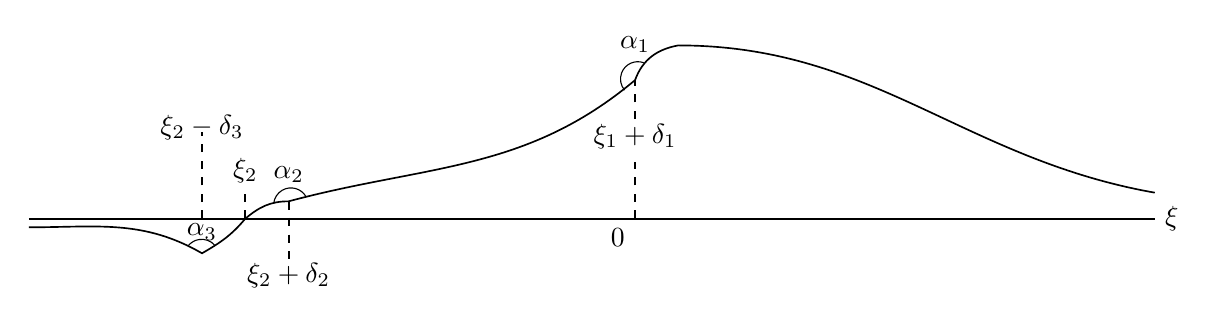
\begin{tikzpicture}[scale = 1.1]
\draw[thick](-6,0) -- (7,0) node[right] {$\xi$};
\draw [semithick] (-6, -0.1) to [ out=0, in=150] (-4,-0.4) to [out=30, in=230] (-3.5,0)  to [out= 40, in=180] (-3,0.2) to [out=15, in=220] (1,1.6) to [out=70,in=190] (1.5,2) to [out=0,in=170] (7,0.3);
\node[below] at (1,1.2) {$\xi_{1}+\delta_1$};
\node[below] at (0.8,0) {$0$};
\draw[dashed] [thick] (-3.5,0)-- (-3.5,0.3);
\node[above] at (-3.5,0.3) {$\xi_2$};
\draw[dashed] [thick] (-3,0.2)-- (-3,-0.5);
\draw[dashed] [thick] (-4,0)-- (-4,1);
\node[above] at (-4,0.8) {$\xi_2-\delta_3$};
\draw[dashed] [thick] (1,0)-- (1,0.65);
\draw[dashed] [thick] (1,1.15)-- (1,1.6);
\node[below] at (-3,-0.4) {$\xi_2+\delta_2$};
\draw [thin] (-3.85,-0.31) arc [radius=0.2, start angle=40, end angle= 140];
\node[above] at (-4,-0.36) {$\alpha_3$};
%\draw [thin] (-2.3,0.355) arc [radius=0.2, start angle=30, end angle= 175];
%\node[above] at (-2.5,0.35) {$\alpha_4$};
\draw [thin] (-2.8,0.255) arc [radius=0.2, start angle=30, end angle= 175];
\node[above] at (-3,0.3) {$\alpha_2$};
\draw [thin] (1.1,1.8) arc [radius=0.2, start angle=70, end angle= 220];
\node[above] at (1,1.8) {$\alpha_1$};
%\node[above] at (2.5,0.5) {\Large{$R_w$}};
%\node[below] at (1,-1.3) {Figure \ref{Figure scalar nl}: the construction of $\mathcal{R}_w(\xi)$.};
\end{tikzpicture}
\caption{the construction of $\mathcal{R}_w(\xi)$.}\label{Figure scalar nl}
\end{center}
\end{figure}


Let $\xi_1,\xi_2$ be chosen like that in Lemma \ref{lm: divide R to 3 parts}. Similar as $R_w(\xi)$, we shall construct auxiliary function $\mathcal{R}_w(\xi)$ (also see Figure \ref{Figure scalar nl}) as follows:
\begin{equation}\label{definition of Rw nonlocal}
\mathcal{R}_w(\xi)=\begin{cases}
\varepsilon_1\sigma(\xi) e^{-\lambda_0\xi},&\ \ \mbox{for}\ \ \xi\ge\xi_{1}+\delta_1,\\
\varepsilon_2 e^{\lambda_1\xi},&\ \ \mbox{for}\ \ \xi_{2}+\delta_2\le\xi\le\xi_{1}+\delta_1,\\
\varepsilon_3\sin(\delta_4(\xi-\xi_2)),&\ \ \mbox{for}\ \ \xi_2-\delta_3\le\xi\le\xi_2+\delta_2,\\
-\varepsilon_4e^{\lambda_2\xi},&\ \ \mbox{for}\ \ \xi\le\xi_2-\delta_3,
\end{cases}
\end{equation}
where $\delta_{i=1,\cdots,4}>0$, $\lambda_{n=1,2}>0$, and $\sigma(\xi)>0$ will be
determined such that $\bar{\mathcal{W}}(\xi)$ satisfies \eqref{tw super solution scalar nonlocal}. Moreover, we should choose
$\varepsilon_{j=1,\cdots,4}\ll A_0$ ($A_0$ is defined in \eqref{AS-U-infty-for-contradiction scalar nonlocal}) such that $\mathcal{R}_w(\xi)\ll {\mathcal{W}}_*(\xi)$ and $\bar{\mathcal{W}}(\xi)$ is continuous for all $\xi\in\mathbb{R}$.


Since $f(\cdot;q^*)\in C^2$, there exist $K_1>0$ and $K_2>0$ such that
\bea\label{K1K2 nonlocal}
|f''({\mathcal{W}}_*(\xi);q^*)|< K_1,\quad |f'({\mathcal{W}}_*(\xi);q^*)|< K_2\quad \mbox{for all}\quad\xi\in\mathbb{R}.
\eea
%$|f''(W_*(\xi);s^*)|< K_1$ and
%$|f'(W_*(\xi);s^*)|< K_2$ for all $\xi\in\mathbb{R}$.
We set $\lambda_1>0$ %($L_0$ is defined in (A2))
large enough such that
\begin{equation}\label{condition on lambda 1 nonlocal}
-c_0^*\lambda_1+1+K_2<0\ \text{and}\ \lambda_1>\frac{4K_2}{c_0^*}.
\end{equation}

Furthermore, there exists $K_3>0$ such that
\begin{equation}\label{condition on xi_2 scalar nonlocal}
f'({\mathcal{W}}_*(\xi); q^*)\le -K_3<0\quad\text{for all}\quad\xi\le \xi_2.
\end{equation}
Since the kernel $J$ has a compact support, without loss of generality, we assume $J\ge0$ on $[-L,L]$, and $J=0$ for $x\in(-\infty,-L)]\cup[L,\infty)$.
We define $\tilde\lambda=\lambda_{q^*,c^*_0}$ which is the unique positive root obtained from Proposition \ref{prop: asy tw - infty nonlocal} with $q=q^*$ and $c=c^*_0$.
Then, by setting $0<\lambda_2<\tilde\lambda$ sufficiently small, we have
\bea\label{lambda 2 nonlocal}
1+K_3-e^{\lambda_2L}-c_0^*\lambda_2>0.
\eea

We now divide the proof into several steps.

\noindent{\bf{Step 1}:} We consider $\xi\in[\xi_1+\delta_1,\infty)$ where $\delta_1>0$ is small enough and will be determined in Step 2.
In this case, we have
\beaa
\mathcal{R}_w(\xi)=\varepsilon_1\sigma(\xi)\ e^{-\lambda_0\xi}
\eeaa
for some small $\varepsilon_1\ll A_0$.



Note that $\mathcal{W}_*$ satisfies \eqref{scalar nonlocal tw-parameter s} with $c=c_0^*$.
By some  straightforward computations , we have
\begin{equation}\label{N0 inequality step 1 nonlocal}
\begin{aligned}
\mathcal{N}_0[\bar{\mathcal{W}}]=&-J\ast \mathcal{R}_w+\mathcal{R}_w-c_0^*\mathcal{R}'_w-f(\mathcal{W}_*;q^*)+f(\mathcal{W}_*-\mathcal{R}_w;q^*+\delta_0)\\
=&-J\ast \mathcal{R}_w+\mathcal{R}_w-c_0^*\mathcal{R}'_w-f(\mathcal{W}_*;q^*)+f(\mathcal{W}_*-\mathcal{R}_w;q^*)\\
&-f(\mathcal{W}_*-\mathcal{R}_w;q^*)+f(\mathcal{W}_*-\mathcal{R}_w;q^*+\delta_0).
\end{aligned}
\end{equation}
By assumption (A1), (A2), and the statement (1) of Lemma \ref{lm: divide R to 3 parts}, since $\mathcal{W}_*\ll 1$ and $\mathcal{R}_w\ll \mathcal{W}_*$ for $\xi\in[\xi_1+\delta_1,\infty)$, we have
\begin{equation}\label{estimate 1 nonlocal}
-f(\mathcal{W}_*;q^*)+f(\mathcal{W}_*-\mathcal{R}_w;q^*)= -\mathcal{R}_w+f''(0;q^*)(\frac{\mathcal{R}^2_w}{2}-\mathcal{W}_*\mathcal{R}_w)+o((\mathcal{W}_*)^2),
\end{equation}
\begin{equation}\label{estimate 2 nonlocal}
-f(\mathcal{W}_*-\mathcal{R}_w;q^*)+f(\mathcal{W}_*-\mathcal{R}_w;q^*+\delta_0)\le C_1\delta_0(\mathcal{W}_*-\mathcal{R}_w)^2+o((\mathcal{W}_*)^2).
\end{equation}

From \eqref{formula of c_NL}, \eqref{K1K2 nonlocal}, \eqref{N0 inequality step 1 nonlocal}, \eqref{estimate 1 nonlocal}, \eqref{estimate 2 nonlocal}, and Lemma \ref{lm: divide R to 3 parts}, we have
\begin{equation}\label{estimate 4 nonlocal}
\begin{aligned}
\mathcal{N}_0[\bar{\mathcal{W}}]\le &-\varepsilon_1e^{-\lambda_0\xi}\Big(\int_{\mathbb{R}}J(y)[\sigma(\xi-y)-\sigma(\xi)] e^{\lambda_0y}dy\Big)-c^*_0\sigma'e^{-\lambda_0\xi}\\
&+K_1(\frac{\mathcal{R}_w^2}{2}+\mathcal{W}_*\mathcal{R}_w)+C_1\delta_0\mathcal{W}_*^2+o((\mathcal{W}_*)^2.
\end{aligned}
\end{equation}
Let $I_1(\lambda)$ be defined as \eqref{nonlocal root}. Since $(I_1(\lambda)/\lambda)'=0$ when $\lambda=\lambda_0$, from \eqref{formula of c_NL}, we get
\begin{equation}\label{c*0 formula}
c^*_0=\int_{\mathbb{R}}yJ(y)e^{\lambda_0y}dy.
\end{equation}
Then, it follows from \eqref{estimate 4 nonlocal} and \eqref{c*0 formula} that
\begin{equation}\label{estimate 3 nonlocal}
\begin{aligned}
\mathcal{N}_0[\bar{\mathcal{W}}]\le &-\varepsilon_1e^{-\lambda_0\xi}\int_{\mathbb{R}}J(y)[\sigma(\xi-y)-\sigma(\xi)+y\sigma'(\xi)] e^{\lambda_0y}dy\\
&+K_1(\frac{\mathcal{R}_w^2}{2}+\mathcal{W}_*\mathcal{R}_w)+C_1\delta_0\mathcal{W}_*^2+o((\mathcal{W}_*)^2.
\end{aligned}
\end{equation}

Now, we define
$$\sigma(\xi):=\frac{1}{\lambda_0^2}e^{-\frac{\lambda_0}{2}(\xi-\xi_1)}-\frac{1}{\lambda_0^2}+\frac{1}{\lambda_0}\xi-\frac{1}{\lambda_0}\xi_1$$
which satisfies 
$$\sigma(\xi_1)=0,\ \sigma'(\xi)=\frac{1}{\lambda_0}-\frac{1}{2\lambda_0}e^{-\frac{\lambda_0}{2}(\xi-\xi_1)}.$$
 Moreover, $\sigma(\xi)= O(\xi)$ as $\xi\to\infty$ implies that $\mathcal{R}_w$ satisfies \eqref{decay rate of Rw nonlocal}.

By some straightforward computation, we have
\begin{equation*}
\int_{\mathbb{R}}J(y)[\sigma(\xi-y)-\sigma(\xi)+y\sigma'(\xi)] e^{\lambda_0y}dy=\frac{1}{\lambda_0^2}e^{-\frac{\lambda_0}{2}(\xi-\xi_1)}\int_{\mathbb{R}}J(y)e^{\lambda_0 y}[e^{\frac{\lambda_0y}{2}}-1-\frac{\lambda_0y}{2}]dy.
\end{equation*}
Notice that, the function 
$$g(y):=e^{\frac{\lambda_0y}{2}}-1-\frac{\lambda_0y}{2}\ge 0$$
 is convex and obtains minimum at $y=0$. Therefore, we assert that there exists $K_4>0$ independent on $\xi_1$ such that
\begin{equation}\label{estimate K4 nonlocal}
-\varepsilon_1e^{-\lambda_0\xi}\int_{\mathbb{R}}J(y)[\sigma(\xi-y)-\sigma(\xi)+y\sigma'(\xi)] e^{\lambda_0y}dy\le -\varepsilon_1K_4e^{-\lambda_0\xi}e^{\frac{\lambda_0(\xi-\xi_1)}{2}}.
\end{equation}



Due to \eqref{AS-U-infty-for-contradiction scalar nonlocal} and the equation of $\mathcal{W}_*$, we may also assume
\bea\label{W-M nonlocal}
\mathcal{W}_*(\xi) \leq 2A_0\xi e^{-\lambda_0\xi}\quad \mbox{for all}\quad\xi\geq \xi_1.
\eea
Then, from \eqref{estimate 3 nonlocal} and \eqref{estimate K4 nonlocal}, up to enlarging $\xi_1$ if necessary, we always have %can find a small $\delta_0>0$ such that
\beaa
\mathcal{N}_0[\bar{\mathcal{W}}]\le -\varepsilon_1K_4e^{-\frac{\lambda_0}{2}(\xi-\xi_1)}e^{-\lambda_0\xi}+K_1(\frac{\mathcal{R}_w^2}{2}+\mathcal{W}_*\mathcal{R}_w)+C_1\delta_0\mathcal{W}_*^2+o((\mathcal{W}_*)^2)\le 0
\eeaa
for all sufficiently small $\delta_0>0$
since $\mathcal{R}_w^2(\xi)$, $\mathcal{W}_*\mathcal{R}_w(\xi)$, and  $\mathcal{W}_*^2(\xi)$ are $o(e^{-\frac{3\lambda_0}{2}\xi})$ for $\xi\ge \xi_1$ from \eqref{W-M nonlocal} and the definition of $\mathcal{R}_w$.
Therefore, $\mathcal{N}_0[\bar{\mathcal{W}}]\leq 0$ for $\xi\ge \xi_1$.


\medskip


\noindent{\bf{Step 2:}} We consider $\xi\in[\xi_2+\delta_2,\xi_1+\delta_1]$ for some small $\delta_2>0$, and sufficiently small $\delta_1>0$ satisfying
\bea\label{cond delta 1 scalar nonlocal}
\frac{3}{2}e^{-\frac{\lambda_0\delta_1}{2}}+\delta_1\lambda_0<2.
\eea
From the definition of $\mathcal{R}_w$ in Step 1, it is easy to check that $\mathcal{R}'_w((\xi_1+\delta_1)^+)>0$ under the condition \eqref{cond delta 1 scalar nonlocal}.
In this case, we have $\mathcal{R}_w(\xi)=\varepsilon_2 e^{\lambda_1\xi}$
for some large $\lambda_1>0$ satisfying \eqref{condition on lambda 1 nonlocal}.

We first choose
\begin{equation}\label{condition on epsilon 2}
\varepsilon_2=\frac{\varepsilon_1}{\lambda^2_0}\Big(e^{-\frac{\lambda_0\delta_1}{2}}-1+\delta_1\lambda_0\Big)e^{-(\lambda_0+\lambda_1)(\xi_1+\delta_1)}
\end{equation}
such that $\mathcal{R}_w(\xi)$ is continuous at $\xi=\xi_{1}+\delta_1$. Then, from \eqref{condition on epsilon 2}, we have
$$\mathcal{R}'_w((\xi_1+\delta_1)^{+})=\varepsilon_1\sigma'(\xi_1+\delta_1)e^{-\lambda_0(\xi_1+\delta_1)}- \lambda_0\mathcal{R}_w(\xi_1+\delta_1),$$
$$\mathcal{R}'_w((\xi_1+\delta_1)^{-})=\lambda_1\mathcal{R}_w(\xi_1+\delta_1),$$
and $\mathcal{R}'_w((\xi_1+\delta_1)^{+})>\mathcal{R}'_w((\xi_1+\delta_1)^{-})$ is equivalent to
$$2(\lambda_0+\lambda_1)(e^{-\frac{\lambda_0\delta_1}{2}}-1+\delta_1\lambda_0)+\lambda_0e^{-\frac{\lambda_0\delta_1}{2}}<2\lambda_0,$$
which holds by taking $\delta_1$ sufficiently small.
This implies that $\angle\alpha_1<180^{\circ}$.

Since $J\ast \mathcal{R}_w\ge 0$, by some  straightforward computations, we have
\begin{equation*}
\begin{aligned}
\mathcal{N}_0[\bar{\mathcal{W}}]
\le&-(c_0^*\lambda_1-1)\mathcal{R}_w-f(\mathcal{W}_*;q^*)+f(\mathcal{W}_*-\mathcal{R}_w;q^*)\\
&-f(\mathcal{W}_*-\mathcal{R}_w;q^*)+f(\mathcal{W}_*-\mathcal{R}_w;q^*+\delta_0).
\end{aligned}
\end{equation*}
%For $\xi\in[\xi_2+\delta_2,\xi_1+\delta_1]$,
Thanks to \eqref{K1K2 nonlocal}, we have
$$-f(\mathcal{W}_*;q^*)+f(\mathcal{W}_*-\mathcal{R}_w;q^*)< K_2\mathcal{R}_w.$$
Moreover, by assumption (A2), %there exists $C_2>0$ such that
$$-f(\mathcal{W}_*-\mathcal{R}_w;q^*)+f(\mathcal{W}_*-\mathcal{R}_w;q^*+\delta_0)\le L_0\delta_0.$$
Then, %by setting
since
$\lambda_1$ satisfies \eqref{condition on lambda 1 nonlocal}, we have
$$L_0\delta_0<\varepsilon_2(c_0^*\lambda_1-1-K_2) e^{\lambda_1(\xi_2+\delta_2)}$$
for all sufficiently small $\delta_0>0$,
which implies that $\mathcal{N}_0[\bar{\mathcal W}]\le 0$ for all $\xi\in[\xi_2+\delta_2,\xi_1+\delta_1]$.


\medskip


\noindent{\bf{Step 3:}} We consider $\xi\in[\xi_2-\delta_3,\xi_2+\delta_2]$ for some small $\delta_2,\delta_3>0$. In this case, we have $\mathcal{R}_w=\varepsilon_3\sin(\delta_4(\xi-\xi_2))$.
We obtain the following Claim by applying the same argument as Claim \ref{cl scalar}.
\begin{claim}\label{cl scalar nonlocal}
For any $\delta_2$ with $\delta_2>\frac{1}{\lambda_1}$, there exist
$\varepsilon_3>0$ and small $\delta_4>0$ satisfying
\bea\label{epsilon 3 nonlocal}
\varepsilon_3= \frac{\varepsilon_2e^{\lambda_1(\xi_2+\delta_2)}}{\sin(\delta_4\delta_2)}>0
\eea
such that $\mathcal{R}_w((\xi_2+\delta_2)^+)=\mathcal{R}_w((\xi_2+\delta_2)^-)$ and $\angle\alpha_2<180^{\circ}$.
\end{claim}


Next, we verify the differential inequality of $\mathcal{N}_0[\bar{\mathcal W}]$ for $\xi\in[\xi_2-\delta_3,\xi_2+\delta_2]$.
Since the kernel $J$ has a compact support,
by some straightforward computations, we have
\begin{equation*}
\begin{aligned}
\mathcal{N}_0[\bar{\mathcal W}]=&\varepsilon_3\int_{-L}^LJ(y)\Big(\sin(\delta_4(\xi-\xi_2)-\sin(\delta_4(\xi-y-\xi_2))\Big)dy-c_0^*\varepsilon_3\delta_4\cos(\delta_4(\xi-\xi_2))\\
&-f(\mathcal{W}_*;s^*)+f(\mathcal{W}_*-\mathcal{R}_w;s^*)-f(\mathcal{W}_*-\mathcal{R}_w;s^*)+f(\mathcal{W}_*-\mathcal{R}_w;s^*+\delta_0)\\
\le &\varepsilon_3\int_{-L}^LJ(y)\Big(\sin(\delta_4(\xi-\xi_2))-\sin(\delta_4(\xi-y-\xi_2))\Big)dy\\
&+K_2\sin(\delta_4(\xi-\xi_2))-c_0^*\varepsilon_3\delta_4\cos(\delta_4(\xi-\xi_2))+L_0\delta_0.
\end{aligned}
\end{equation*}
%The same argument as in Step 2 implies that
%$$-f(W_*;s^*)+f(W_*-R_w;s^*)\le K_2R_w\quad\text{and}\quad -f(W_*-R_w;s^*)+f(W_*-R_w;s^*+\delta_0)\le L_0\delta_0,$$
%which yields that
%\beaa
%N_0[\bar W]\leq &\delta^2_4R_w-2\varepsilon_3\delta_4\cos(\delta_4(\xi-\xi_2))+K_2R_w+L_0\delta_0.
%\eeaa

We first focus on $\xi\in[\xi_2,\xi_2+\delta_2]$. Since the integral is defined on a bounded domain and we always set $\delta_4$ small, up to decreasing $\delta_4$ if necessary, by Taylor series, we have
$$\sin(\delta_4(\xi-\xi_2-y))-\sin(\delta_4(\xi-\xi_2))\approx-y\delta_4^2\cos(\delta_4(\xi-\xi_2))-\frac{y^2\delta_4^4}{2}\sin(\delta_4(\xi-\xi_2)).$$
Then, by setting $\delta_4<c_0^*/2L$,
\begin{equation}\label{inequilty 1}
|y\delta_4^2\cos(\delta_4(\xi-\xi_2))|<c_0^*\delta_4\cos(\delta_4(\xi-\xi_2))/2.
\end{equation}
Therefore, we obtain
\begin{equation}\label{inequality 2}
\mathcal{N}_0[\bar{\mathcal W}]\le -\varepsilon_3\frac{c_0^*\delta_4}{2}\cos(\delta_4(\xi-\xi_2))+(K_2+\frac{L^2\delta_4^4}{2})\sin(\delta_4(\xi-\xi_2))+L_0\delta_0.
\end{equation}

By \eqref{epsilon 3 nonlocal} and the fact $x\cos x\to\sin x$ as $x\to 0$,
\beaa
\min_{\xi\in[\xi_2,\xi_2+\delta_2]}\frac{\delta_4\varepsilon_3c_0^*}{2}\cos(\delta_4(\xi-\xi_2))\to\frac{c_0^*\varepsilon_2e^{\lambda_1(\xi_2+\delta_2)}}{2\delta_2}
=\frac{c^*_0\mathcal{R}_w(\xi_2+\delta_2)}{2\delta_2}
\quad\text{as}\ \delta_4\to0.
\eeaa
Then, by \eqref{condition on lambda 1 nonlocal}, we can choose
$\delta_2\in(1/\lambda_1,c_0^*/4K_2)$ such that
%yields that
\beaa
\frac{c^*_0\mathcal{R}_w(\xi_2+\delta_2)}{2\delta_2}>2 K_2\mathcal{R}_w(\xi_2+\delta_2)
\quad\text{as}\ \delta_4\to0.
\eeaa
%We take $\delta_2<1/\lambda_1$ which is arbitrarily small since \eqref{condition on lambda 1}.
Thus, we have
\beaa%\label{Rv-estimate}
\min_{\xi\in[\xi_2,\xi_2+\delta_2]}\frac{\delta_4\varepsilon_3c_0^*}{2}\cos(\delta_4(\xi-\xi_2))>(K_2+\frac{L^2\delta_4^4}{2})\mathcal{R}_w(\xi),
\eeaa
for all sufficiently small $\delta_4>0$.
Then, from \eqref{inequality 2}, for all sufficiently small $\delta_0>0$, %sufficiently small,
we see that $\mathcal{N}_0[\bar{\mathcal W}]\le 0$ for $\xi\in[\xi_2,\xi_2+\delta_2]$.

For $\xi\in[\xi_2-\delta_3,\xi_2]$, by the same argument
we can set $\delta_3>0$ small enough such that
$\mathcal{N}_0[\bar{\mathcal W}]\le 0$. This completes the Step 3.

\medskip

\noindent{\bf{Step 4:}} We consider $\xi\in(-\infty,\xi_2-\delta_3]$. In this case, we have $\mathcal{R}_w(\xi)=-\varepsilon_4e^{\lambda_2\xi}<0$.
Recall that we choose $0<\lambda_2<\tilde\lambda$
and 
$$1-\mathcal{W}_*(\xi)\approx C_2 e^{\tilde\lambda\xi}\ \ \text{as}\ \ \xi\to-\infty.$$
Then, there exists $M>0$ such that 
$$\bar{\mathcal W}:=\min\{\mathcal{W}_*-\mathcal{R}_w,1\}\equiv 1\ \ \text{for all}\ \ \xi\le -M,$$
and thus 
$$\mathcal{N}_0[\bar{\mathcal W}]\le 0\  \ \text{for all}\ \ \xi\le -M.$$ Therefore, we only need to show 
$$\mathcal{N}_0[\bar{\mathcal W}]\le 0\ \  \text{for all}\ \ -M\le\xi\le -\xi_2-\delta_3.$$

We first choose 
$$\varepsilon_4=\varepsilon_3\sin(\delta_4\delta_3)/e^{\lambda_2(\xi_2-\delta_3)}$$
such that $\mathcal{R}_w$ is continuous at $\xi_2-\delta_3$. It is easy to check that 
$$\mathcal{R}'_w((\xi_2-\delta_3)^+)>0>\mathcal{R}'_w((\xi_2-\delta_3)^-)$$
 and so $\angle\alpha_3< 180^{\circ}$.

Since the kernel $J$ is only defined on $[-L,L]$, by some straightforward computations, we have
\begin{equation*}
\begin{aligned}
\mathcal{N}_0[\bar{\mathcal W}]
\le&-(e^{\lambda_2L}+c_0^*\lambda_2-1)\mathcal{R}_w-f(\mathcal{W}_*;q^*)+f(\mathcal{W}_*-\mathcal{R}_w;q^*)\\
&-f(\mathcal{W}_*-\mathcal{R}_w;q^*)+f(\mathcal{W}_*-\mathcal{R}_w;q^*+\delta_0).
\end{aligned}
\end{equation*}
From \eqref{condition on xi_2 scalar nonlocal}, we have 
$$-f(\mathcal{W}_*;q^*)+f(\mathcal{W}_*-\mathcal{R}_w;q^*)< K_3\mathcal{R}_w<0.$$
Together with (A2), we have
\beaa
\mathcal{N}_0[\bar{\mathcal W}]\leq -(e^{\lambda_2L}+c_0^*\lambda_2-1-K_3)\mathcal{R}_w+L_0\delta_0\quad\text{for all}\quad \xi\in[-M,\xi_2-\delta_3].
\eeaa
In view of \eqref{lambda 2 nonlocal},
we can assert that 
$$\mathcal{N}_0[\bar{\mathcal W}]\le 0\ \ \text{for all}\ \ \xi\in[-M,\xi_2-\delta_3],$$
provided that $\delta_0$ is sufficiently small.
This completes the Step 4.

\subsection{Proof of Theorem \ref{th: threshold scalar equation nonlocal}}

\noindent

We are ready to prove Theorem~\ref{th: threshold scalar equation nonlocal} as follows.

\begin{proof}[Proof of Theorem~\ref{th: threshold scalar equation nonlocal}]
In view of Lemma~\ref{lem: th1-part1 nonlocal}, we have obtained \eqref{def of threshold scalar nonlocal}.
It suffices to show that \eqref{asy tw threshold scalar nonlocal} holds if and only if $q=q^*$.
From the discussion from the Step 1 to Step 4 in \S \ref{subsec-3-1},
we are now equipped with an auxiliary function $\mathcal{R}_w(\xi)$ %well defined for all
defined as in \eqref{definition of Rw nonlocal} such that 
$$\bar{\mathcal W} (\xi)=\min \{\mathcal{W}_*(\xi)-\mathcal{R}_w(\xi),1\},$$
 which is independent of the choice of all sufficiently small $\delta_0>0$, forms
a super-solution satisfying \eqref{tw super solution scalar nonlocal}. By the argument used in the proof of Theorem \ref{th: threshold scalar equation}, similarly we can show
\bea\label{th1:goal-1 nonlocal}
q=q^* \quad \Longrightarrow \quad \mbox{\eqref{asy tw threshold scalar nonlocal} holds}.
\eea
Therefore, it suffice to prove
\bea\label{th1:goal-2 nonlocal}
\mbox{\eqref{asy tw threshold scalar} holds} \quad \Longrightarrow \quad q=q^*
\eea
by the same argument as that in the proof of Theorem \ref{th: threshold scalar equation}.

We assume by contradiction that there exists $q_0\in(0,q^*)$ such that
the corresponding minimal traveling wave satisfies
\bea\label{W-S0+infty nonlocal}
\mathcal{W}_{q_0}(\xi)=B_0 e^{-\lambda_0\xi}+o(e^{-\lambda_0\xi})\quad\text{as}\quad \xi\to+\infty
\eea
for some $B_0>0$. For $\xi\approx -\infty$, from Proposition \ref{prop: asy tw - infty nonlocal}, we have
\bea\label{W-S0-infty nonlocal}
1-\mathcal{W}_{q_0}(\xi)=C_0 e^{\tilde\lambda_0\xi}+o(e^{\tilde\lambda_0\xi})\quad\text{as}\quad \xi\to-\infty
\eea
for some $C_0>0$, where $\tilde\lambda_0=\lambda_{s_0,c_0^*}$.
Recall that the asymptotic behavior of $\mathcal{W}_q^*$ at $\pm\infty$ satisfies
\bea\label{W-S*-pm-infty nonlocal}
\mathcal{W}_{q^*}(\xi)=B e^{-\lambda_0\xi}+o(e^{-\lambda_0\xi})\ \text{as}\ \xi\to+\infty;\ \ 1-\mathcal{W}_{q^*}(\xi)=C e^{\tilde\lambda\xi}+o(e^{\tilde\lambda\xi})\ \text{as}\ \xi\to-\infty
\eea
for some $B,C>0$, where $\tilde\lambda=\lambda_{q^*,c^*_0}$. In view of assumption (A3), we have $\tilde\lambda>\tilde\lambda_0$ since $q^*>q_0$.
Combining \eqref{W-S0+infty nonlocal}, \eqref{W-S0-infty nonlocal} and \eqref{W-S*-pm-infty nonlocal}, there exists $L>0$ sufficiently large such that
$\mathcal{W}_{q^*}(\xi-L)> \mathcal{W}_{q_0}(\xi)$ for all $\xi\in\mathbb{R}$. Now, we define
\beaa
L^*:=\inf\{L\in\mathbb{R}\ |\ \mathcal{W}_{q^*}(\xi-L)\ge \mathcal{W}_{q_0}(\xi)\ \text{for all}\ \xi\in\mathbb{R}\}.
\eeaa
By the continuity, we have 
$$\mathcal{W}_{q^*}(\xi-L^*)\geq \mathcal{W}_{q_0}(\xi)\ \text{for all}\ \ \xi\in\mathbb{R}.$$
 If there exists $\xi^*\in\mathbb{R}$ such that
$\mathcal{W}_{q^*}(\xi^*-L^*)= \mathcal{W}_{q_0}(\xi^*)$, by the strong maximum principle, we have 
$$\mathcal{W}_{q^*}(\xi-L^*)=\mathcal{W}_{q_0}(\xi)\ \ \text{for}\ \ \xi\in\mathbb{R},$$
which is impossible since $\mathcal{W}_{q^*}(\cdot-L^*)$ and $\mathcal{W}_{q_0}(\cdot)$ satisfy different equations. Consequently,
$$\mathcal{W}_{q^*}(\xi-L^*)> \mathcal{W}_{q_0}(\xi)\ \ \text{for all}\ \ \xi\in\mathbb{R}.$$ 
In particular, we have
\beaa
\lim_{\xi\to\infty}\frac{\mathcal{W}_{q^*}(\xi-L^*)}{\mathcal{W}_{q_0}(\xi)}\geq1.
\eeaa
Furthermore, we can claim that
\bea\label{limit=1 nonlocal}
\lim_{\xi\to\infty}\frac{\mathcal{W}_{q^*}(\xi-L^*)}{\mathcal{W}_{q_0}(\xi)}=1.
\eea
%\red{
%To prove this, we first claim that it either
%\beaa
%\lim_{\xi\to\infty}\frac{W_{s^*}(\xi-L^*)}{W_{s_0}(\xi)}=1\quad\text{or}\quad\lim_{\xi\to-\infty}\frac{1-W_{s^*}(\xi-L^*)}{1-W_{s_0}(\xi)}=1.
%\eeaa
Otherwise, if the limit in \eqref{limit=1 nonlocal} is strictly bigger than 1, together with
\bea\label{(1-W)-decay nonlocal}
\lim_{\xi\to-\infty}\frac{1-\mathcal{W}_{q^*}(\xi-L^*)}{1-\mathcal{W}_{q_0}(\xi)}=0,
\eea
%we can use a standard argument (see, e.g., \cite{Hamel Roques}) to
we can easily  find $\varepsilon>0$ sufficiently small such that
$$\mathcal{W}_{q^*}(\xi-(L^*+\varepsilon))> \mathcal{W}_{q_0}(\xi)\ \ \text{for all}\ \ \xi\in\mathbb{R},$$
which contradicts the definition of $L^*$.
%Notice that,
%\beaa
%\lim_{\xi\to-\infty}\frac{1-W_{s^*}(\xi-L^*)}{1-W_{s_0}(\xi)}=1
%\eeaa
%can never happen since $1-W_{s^*}\approx C_1e^{\nu_1\xi}$, $1-W_{s_0}\approx C_2e^{\nu_2\xi}$, and $\nu_1>\nu_2$  which follows from $s^*>s_0$ and the assumptions (A1)(A3).
As a result, from \eqref{W-S0+infty nonlocal}, \eqref{W-S*-pm-infty nonlocal} and \eqref{limit=1 nonlocal}, we obtain $B_0=Be^{L^*}$.


On the other hand, by considering the equation satisfied by $\widehat{\mathcal{W}}(\xi)=\mathcal{W}_{q^*}(\xi-L^*)-\mathcal{W}_{q_0}(\xi)$ and $B_0=Be^{L^*}$,
the asymptotic behavior of $\widehat{\mathcal{W}}(\xi)$ at $\xi=+\infty$ satisfies
\beaa
\widehat{\mathcal{W}}(\xi)=(C_1\xi+C_2)e^{-\beta \xi}+o(e^{-\beta\xi})\quad \mbox{as $\xi\to\infty$},
\eeaa
where  $C_1=0$ and $C_2=0$, which reaches a contradiction to Proposition \ref{prop:correction-U-linear-decay}.
Therefore, \eqref{th1:goal-2 nonlocal} holds, and the proof is complete.
\end{proof}

\section{Classification of the minimal traveling wave}\label{sec:classification}

In this section, we conclude the main results of this paper, and complete the proof of Corollary \ref{cor: different minimal tw}, \ref{cor: different minimal tw system}, and \ref{cor: different minimal tw nonlocal}.

In Section \ref{sec:threshold scalar}, we studied the transition between the speed linear selection and nonlinear selection by considering the single monostable reaction-diffusion equation 
$$w_t=w_{xx}+f(w;s)$$
with a family of continuously increasing nonlinearity $f(w;s)$ satisfying (A1)-(A5). 
The eigenfunction $\lambda^2-c^*(s)\lambda+f'(0;s)=0$, derived from the linearization of minimal traveling wave solutions
$W''+c^*(s)W'+f(W;s)=0$ at $W\approx 0$, admits 
\begin{itemize}
\item one double root $\lambda=\sqrt{f'(0)}$ if $c^*(s)=2\sqrt{f'(0)}$, 
\item two single roots 
$$\lambda_s^{\pm}=\frac{c^*(s)\pm\sqrt{(c^*(s))^2-4f'(0)}}{2}\ \ \text{if}\ \ c^*(s)>2\sqrt{f'(0)}.$$ 
\end{itemize}

By the classical ODE argument, for the case $s\in (0,s^*]$, $c^*(s)=2\sqrt{f'(0)}$ and the asymptotic behavior of the pulled front is given by the linear combination of eigenvectors $\xi e^{-\sqrt{f'(0)}\xi}$ and  $e^{-\sqrt{f'(0)}\xi}$. More importantly, we found that the decay rate of the minimal traveling wave changes to $e^{-\sqrt{f'(0)}\xi}$ if and only if $s=s^*$ which is the threshold between speed linear selection and nonlinear selection. Therefore, the first and the second statements of Corollary \ref{cor: different minimal tw} follow immediately from Theorem \ref{th: threshold scalar equation}. On the other hand, for $s>s^*$, the propagation speed is nonlinearly selected $c^*(s)>2\sqrt{f'(0)}$. Furthermore, it can be proved by the basic phase plane analysis that the asymptotic behavior of the pushed front is given by the fast decay $e^{-\lambda_s^+\xi}$, i.e. statement (3) of Corollary \ref{cor: different minimal tw}.

In Section \ref{sec:threshold-system}, we studied the transition between speed linear selection and nonlinear selection of the Lotka-Volterra competition system
\begin{equation*}
\left\{
\begin{aligned}
u_t=u_{xx}+u(1-u-av),\\
v_t=dv_{xx}+rv(1-v-bu).
\end{aligned}
\right.
\end{equation*}
Note that,  in Section \ref{sec: sufficient condition 1}, we established a condition (see Theorem \ref{th:large-d}) under which the speed is nonlinearly selected for certain values of $0<a,b<1$. Therefore, to fully capture the entire process of how the speed transitions from linear selection to nonlinear selection, it is crucial to consider this problem within the extended parameter range of $0<a<1$ and $b>0$, rather than just $0<a<1$ and $b>1$ (the so-called strong-weak competition case).  The eigenfunction $\lambda^2-c^*(s)\lambda+1-a=0$, derived from the linearization of minimal traveling wave solutions
$U''+c_{LV}^*(b)U'+U(1-U-aV)=0$ at $(U,V)\approx (0,1)$, admits 
\begin{itemize}
\item one double root $\lambda=\sqrt{1-a}$ if $c^*_{LV}(b)=2\sqrt{1-a}$, 
\item two single roots 
$$\lambda_u^{\pm}=\frac{c_{LV}^*(b)\pm\sqrt{(c^*_{LV}(b))^2-4(1-a)}}{2}\ \ \text{if}\ \ c_{LV}^*(b)>2\sqrt{1-a}.$$ 
\end{itemize}


Similar to the single equation problem, for the case $b\in (0,b^*]$, we have $c^*_{LV}(b)=2\sqrt{1-a}$, and the asymptotic behavior of the pulled front is given by the linear combination of eigenvectors $\xi e^{-\sqrt{1-a}\xi}$ and  $e^{-\sqrt{1-a}\xi}$. Importantly,  the decay rate of the minimal traveling wave changes to $e^{-\sqrt{1-a}\xi}$ if and only if $b=b^*$ which is the threshold between speed linear selection and nonlinear selection. Therefore, the first and the second statements of Corollary \ref{cor: different minimal tw system} follow immediately from Theorem \ref{th:threshold}. On the other hand, for $b>b^*$, the propagation speed is nonlinearly selected $c_{LV}^*(b)>2\sqrt{1-a}$. Furthermore, it can be proved by computing the stable invariant manifold that the asymptotic behavior of the pushed front is given by the fast decay $e^{-\lambda_u^+\xi}$ (see \cite{Kan-on1997}), i.e. statement (3) of Corollary \ref{cor: different minimal tw system}.

In Section \ref{sec: threshold scalar nonlocal}, we extended our observation to the integro-differential equation which has a nonlocal diffusion kernel
$$w_t=J\ast w-w+f(w;q)$$
with a family of continuously increasing nonlinearity $f(w;q)$ satisfying (A1)-(A3) and (A6)-(A7). Different with the reaction-diffusion equation, the linearly selected speed is given by a variational formula
$$c_0^*:=\min\frac{1}{\lambda}\Big(\int_{\mathbb{R}}J(x)e^{\lambda x}dx+f'(0;q)-1\Big),$$
which is also derived from the linearization of minimal traveling wave solutions
$J\ast \mathcal{W}+c_{NL}^*(q)\mathcal{W}'+f(\mathcal{W};q)=0$ at $\mathcal{W}\approx 0$. Furthermore, since the function 
$$g(\lambda):=\frac{1}{\lambda}\Big(\int_{\mathbb{R}}J(x)e^{\lambda x}dx+f'(0;q)-1\Big)$$
is positive and strictly concave, 
$c\lambda=\int_{\mathbb{R}}J(x)e^{\lambda x}dx+f'(0;q)-1$ admits
\begin{itemize}
\item one double root $\lambda=\lambda_0$ if $c^*_{NL}( q)=c_0^*$, 
\item two single root $\lambda^{\pm}_q(c)$ satisfying
\begin{equation}\label{two roots}
\lambda^-_q(c)<\lambda_0<\lambda^+_q(c)\ \ \text{if}\ \ c^*_{NL}(q)>c_0^*.
\end{equation}
\end{itemize}

By Ikehara's Theorem, for the case $q\in (0,q^*]$, $c^*_{NL}(q)=c_0^*$ and the asymptotic behavior of the pulled front is given by the linear combination of eigenvectors $\xi e^{-\lambda_0\xi}$ and  $e^{-\lambda_0\xi}$. More importantly, we found that the decay rate of the minimal traveling wave changes to $e^{-\lambda_0\xi}$ if and only if $q=q^*$, which establishes the difference between the pulled front and the pulled-to-pushed front. Therefore, the first and the second statements of Corollary \ref{cor: different minimal tw nonlocal} follow immediately from Theorem \ref{th: threshold scalar equation nonlocal}. On the other hand, for $q>q^*$ when the propagation speed is nonlinearly selected $c_{NL}^*(s)>c_0^*$,  the asymptotic behavior of the pushed front is still an open problem. 


The rest of this section is devoted to completing the proof of Corollary \ref{cor: different minimal tw nonlocal}. We show that the asymptotic behavior of the pushed front is also given by the fast decay $e^{-\lambda^+\xi}$. As a matter of fact, if the pushed front decays with the slow rate $e^{-\lambda^-\xi}$, then we can always construct a traveling wave solution with speed $c<c^*_{NL}$, which contradicts the definition of the minimal speed $c^*_{NL}$. 

In this section, we always assume $c^*_{NL}>c^*_0$ and denote the pushed front by $\mathcal{W}_*(\xi)$.
Then by assuming 
\bea\label{assume}
\mathcal{W}_*(\xi)\sim A_0e^{-\lambda^-\xi}
\eea
which is the smaller root of \eqref{two roots} with $c=c^*_{NL}-\delta_0$,
we can find a sup-solution $\overline{\mathcal{W}}(\xi)$ and a sub-solution $\underline{\mathcal{W}}(\xi)$ of
\begin{equation}\label{N 1}
\mathcal N_1[\mathcal W]:=J\ast \mathcal W+(c^*_{NL}-\delta_0)\mathcal W'-\mathcal W+f(\mathcal W)=0
\end{equation}
with the boundary condition $\overline{\mathcal{W}}(-\infty)=\underline{\mathcal{W}}(-\infty)=1$ and $\overline{\mathcal{W}}(+\infty)=\underline{\mathcal{W}}(+\infty)=0$.
As a result, we can assert that there exists a traveling wave solution with speed $c^*_{NL}-\delta_0$ by applying the iteration argument(see the proof of Theorem 3.1 in \cite{Coville Dupaigne}),  and get the contradiction. In Section \ref{sec:classification}, we denote $c^*:=c^*_{NL}$ for simplicity.


\subsection{Construction of the super-solution}
We first construct the super-solution of \eqref{N 1} which satisfies $\mathcal N_1[\overline{\mathcal W}]\le 0$. The approach is similar to the super-solution \eqref{definition of Rw nonlocal} provided in \S \ref{subsec-3-1}. 

Let $\xi_1,\xi_2$ be chosen like that in Lemma \ref{lm: divide R to 3 parts}. 
We consider a super-solution in the form of (see Figure \ref{Figure sup solution})
\begin{equation*}
\overline{\mathcal W}:=\left\{
\begin{aligned}
&\varepsilon_1e^{-\lambda_*\xi},&\ \ \text{for}\ \ \xi\ge \xi_1,\\
&\mathcal{W}_*(\xi)-\mathcal{R}_w(\xi),&\ \ \text{for}\ \ \xi< \xi_1,
\end{aligned}
\right.
\end{equation*}
in which $\lambda_*\in(\lambda^-(c^*-\delta_0),\lambda^+(c^*-\delta_0))$, $\mathcal{W}_*$ is the pushed front satisfying \eqref{assume},  and $R_w(\xi)$ defined as

\begin{equation*}%\label{definition of Rw pushed}
\mathcal{R}_w(\xi)=\begin{cases}
\varepsilon_2 e^{\lambda_1\xi},&\ \ \mbox{for}\ \ \xi_{2}+\delta_1\le\xi\le\xi_{1},\\
\varepsilon_3\sin(\delta_3(\xi-\xi_2)),&\ \ \mbox{for}\ \ \xi_2-\delta_2\le\xi\le\xi_2+\delta_1,\\
-\varepsilon_4e^{\lambda_2\xi},&\ \ \mbox{for}\ \ \xi\le\xi_2-\delta_2.
\end{cases}
\end{equation*}
Here $\delta_{i=1,2,3}>0$ and $\lambda_{1},\lambda_2>0$ will be
determined such that  $\mathcal{N}_1[\overline{\mathcal{W}}(\xi)]\le 0$. Moreover, we should choose
$\varepsilon_{j=1,2,3}$ very small such that $\overline{\mathcal{W}}(\xi)$ is continuous for all $\xi\in\mathbb{R}$.

\begin{figure}
\begin{center}
\begin{tikzpicture}[scale = 1.25]
\draw[thick](-6,0) -- (4,0) node[right] {$\xi$};
\draw [thick] (-6, 2.5) to(-4,2.5) to [out=-30, in=170] (1.5,1)  to [out=-40,in=170] (4,0.2);
\node[below] at (1.5,0) {$\xi_{1}$};
\node[left] at (-6,2.5) {$1$};
\draw[dashed]  (-6,2.5) -- (4,2.5);
%\node[above] at (-3.5,0.3) {$\xi_2$};
%\draw[dashed] [thick] (-3,0.2)-- (-3,-0.5);
%\draw[dashed] [thick] (-4,0)-- (-4,1);
%\node[above] at (-4,0.8) {$\xi_2-\delta_3$};
%\draw[dashed] [thick] (1,0)-- (1,0.65);
\draw[dashed] [thick] (1.5,0)-- (1.5,0.5);
%\node[below] at (-3,-0.4) {$\xi_2+\delta_2$};
%\draw [thin] (-3.85,-0.31) arc [radius=0.2, start angle=40, end angle= 140];
%\node[above] at (-4,-0.36) {$\alpha_3$};
%\draw [thin] (-2.3,0.355) arc [radius=0.2, start angle=30, end angle= 175];
%\node[above] at (-2.5,0.35) {$\alpha_4$};
%\draw [thin] (-2.8,0.255) arc [radius=0.2, start angle=30, end angle= 175];
%\node[above] at (-3,0.3) {$\alpha_2$};
\draw [thin] (1.35,1.03) arc [radius=0.2, start angle=175, end angle= 310];
\node[below] at (1.5,0.8) {$\alpha_1$};
%\node[above] at (2.5,0.5) {\Large{$R_w$}};
%\node[below] at (1,-1.3) {Figure \ref{Figure scalar}: the construction of $R_w(\xi)$.};
\end{tikzpicture}
\caption{the super-solution $\overline{\mathcal{W}}(\xi)$.}\label{Figure sup solution}
\end{center}
\end{figure}


Since $f(\cdot)\in C^2$, there exists $K_1>0$  such that
\bea\label{K1K2 nonlocal pushed}
|f'({\mathcal{W}}_*(\xi))|< K_1\quad \mbox{for all}\quad\xi\in\mathbb{R}.
\eea
We set $\lambda_1>0$ %($L_0$ is defined in (A2))
large enough such that
\begin{equation}\label{condition on lambda 1 nonlocal pushed}
c^*\lambda_1>K_1+1\ \text{and}\ \lambda_1>\frac{4K_1}{c^*}.
\end{equation}
Furthermore, there exists $K_2>0$ such that
\begin{equation*}%\label{condition on xi_2 scalar nonlocal pushed}
f'({\mathcal{W}}_*(\xi))\le -K_2<0\quad\text{for all}\quad\xi\le \xi_2.
\end{equation*}
Without loss of generality, we assume $J\ge0$ on $[-L,L]$, and $J=0$ for $x\in(-\infty,-L)]\cup[L,\infty)$.
Let $\tilde\lambda$ be the unique positive root obtained from Proposition \ref{prop: asy tw - infty nonlocal} with $c=c^*_{NL}$.
Additionally, we set
\beaa\label{lambda 2 nonlocal pushed}
0<\lambda_2<\tilde\lambda\ \ \text{and}\ \ 1+K_2-e^{\lambda_2L}-c^*\lambda_2>0.
\eeaa

We now divide the proof into several steps.
\medskip

\noindent{\bf{Step 1}:} We consider $\xi\in[\xi_1,\infty)$ 
In this case, we have
$\overline{\mathcal{W}}(\xi)=\varepsilon_1e^{-\lambda_*\xi}$
for some small $\varepsilon_1$ satisfying 
\begin{equation}\label{varepsilon 1 pushed}
\varepsilon_1e^{-\lambda_*\xi_1}<\mathcal{W}_*(\xi_1)
\end{equation}
and $\lambda_*\in(\lambda^-,\lambda^+)$, where $\lambda^{\pm}$ is defined in \eqref{two roots}.

By Lemma \ref{lm: divide R to 3 parts} and some  straightforward computations,
we have
\begin{equation*}%\label{N1 inequality step 1 nonlocal}
\begin{aligned}
\mathcal{N}_1[\overline{\mathcal{W}}]=&\int_{\mathbb{R}}J(y)\varepsilon_1e^{-\lambda_*(\xi-y)}dy-\varepsilon_1e^{-\lambda_*\xi}-\lambda_*(c^*-\delta_0)\varepsilon_1e^{-\lambda_*\xi}+f(\varepsilon_1e^{-\lambda_*\xi})\\
=&\varepsilon_1e^{-\lambda_*\xi}\Big(\int_{\mathbb{R}}J(y)e^{\lambda_*y}dy-1-\lambda_*(c^*-\delta_0)+f'(0)+o(1)\Big).
\end{aligned}
\end{equation*}
Since $c^*>c^*_0$, by setting $\delta_0$ small such that $c^*-\delta_0>c^*_0$, we can find 
$$\lambda_*\in(\lambda^-(c^*-\delta_0),\lambda^+(c^*-\delta_0))$$
such that
$$\int_{\mathbb{R}}J(y)e^{\lambda_*y}dy-1-\lambda_*(c^*-\delta_0)+f'(0)+o(1)<0.$$
Therefore, $\mathcal{N}_1[\overline{\mathcal{W}}]\leq 0$ for $\xi\ge \xi_1$.
\medskip

\noindent{\bf{Step 2}:} We consider $\xi\in[\xi_2+\delta_1,\xi_1)$ for some small $\delta_1>0$. In this case, we have $\overline{\mathcal{W}}(\xi)=\mathcal{W}_*(\xi)-\mathcal{R}_w(\xi)$ where $\mathcal{R}_w(\xi)=\varepsilon_2 e^{\lambda_1\xi}$
for some large $\lambda_1>0$ satisfying \eqref{condition on lambda 1 nonlocal pushed}.

From the definition of $\overline{\mathcal{W}}$ and \eqref{varepsilon 1 pushed},
we first set $\varepsilon_1$ and $\varepsilon_2$ such that
\begin{equation}\label{eq on var 1 2}
\varepsilon_1e^{-\lambda_*\xi_1}=\mathcal{W}_*(\xi_1)-\varepsilon_2e^{\lambda_1\xi_1},
\end{equation}
which implies $\overline{\mathcal{W}}(\xi)$ is continuous at $\xi=\xi_1$.
It is easy to check that 
\beaa
\overline{\mathcal{W}}'((\xi_1)^+)&=&-\lambda_*\overline{\mathcal{W}}(\xi_1)=-\lambda_*(\mathcal{W}_*(\xi_1)+\mathcal{R}_w(\xi_1)),\\
\overline{\mathcal{W}}'((\xi_1)^-)&=&-\lambda^-\mathcal{W}_*(\xi_1)-\lambda_1\mathcal{R}_w(\xi_1).
\eeaa
Therefore, from \eqref{assume}, $\overline{\mathcal{W}}'((\xi_1)^+)<\overline{\mathcal{W}}'((\xi_1)^-)$ is equivalent to 
\begin{equation*}
\varepsilon_2<\frac{\lambda_*-\lambda^-}{\lambda_*+\lambda_1}A_0e^{-(\lambda^-+\lambda_1)\xi_1},
\end{equation*}
which holds by setting $\varepsilon_1$ suitably in \eqref{eq on var 1 2}.
This implies that $\angle\alpha_1<180^{\circ}$.

Since $J\ast \mathcal{R}_w\ge 0$, by some  straightforward computations, we have
\begin{equation*}
\mathcal{N}_1[\overline{\mathcal{W}}]
\le-((c^*-\delta_0)\lambda_1-1)\mathcal{R}_w-f(\mathcal{W}_*)+f(\mathcal{W}_*-\mathcal{R}_w).
\end{equation*}
%For $\xi\in[\xi_2+\delta_2,\xi_1+\delta_1]$,
Thanks to \eqref{K1K2 nonlocal pushed}, we have
$$-f(\mathcal{W}_*)+f(\mathcal{W}_*-\mathcal{R}_w)< K_1\mathcal{R}_w.$$
Then, 
since
$\lambda_1$ satisfies \eqref{condition on lambda 1 nonlocal pushed} and $\mathcal{R}'_w(\xi)$ is bounded for $\xi\in[\xi_2+\delta_1,\xi_1]$, we have
$$\delta_0|\mathcal{R}'_w(\xi_1)|<\varepsilon_2(c^*\lambda_1-1-K_1) e^{\lambda_1(\xi_2+\delta_1)}$$
for all sufficiently small $\delta_0>0$,
which implies that $\mathcal{N}_1[\bar{\mathcal W}]\le 0$ for all $\xi\in[\xi_2+\delta_1,\xi_1]$.

\medskip

To verify $\mathcal{N}_1[\overline{\mathcal{W}}]\le 0$ for $\xi\in[\xi_2-\delta_2,\xi_2+\delta_1]$ and $\xi\in(-\infty,\xi_2-\delta_2)$, we refer to Step 3 and Step 4 in \S \ref{subsec-3-1}, respectively. Moreover, by \eqref{lambda 2 nonlocal pushed}, we obtain a super-solution  $\overline{\mathcal{W}}$ satisfying the boundary condition
$$\overline{\mathcal{W}}(-\infty)=1\ \ \text{and}\ \ \overline{\mathcal{W}}(+\infty)=0.$$




\subsection{Construction of the sub-solution}
To construct the sub-solution of \eqref{N 1} which satisfies $\mathcal N_1[\underline{\mathcal W}]\ge 0$, we need to use the semi-wave solution which is established in studying the related free boundary problem. 

Let the kernel $J(x)$ satisfy \eqref{assumption on J}.
The nonlocal diffusion model with free boundaries considered in \cite{Du Li Zhou} has the following form:
\begin{equation}\label{nonlocal fb}
\left\{
\begin{aligned}
&u_t=\int_{h_1(t)}^{h_2(t)}J(x-y)u(t,y)dy-u(t,x)+f(u),&\ &t>0,\ x\in[h_1(t),h_2(t)],\\
&u(t,h_1(t))=u(t,h_2(t))=0,&\ &t>0,\\
&h'_1(t)=-\mu\int_{h_1(t)}^{h_2(t)}\int_{-\infty}^{h_1(t)}J(x-y)u(t,x)dydx,&\ &t>0,\\
&h'_2(t)=\mu\int_{h_1(t)}^{h_2(t)}\int^{+\infty}_{h_2(t)}J(x-y)u(t,x)dydx,&\ &t>0,\\
&u(0,x)=u_0(x),\ -h_1(0)=h_2(0)=h_0,&\ &x\in[-h_0,h_0],
\end{aligned}
\right.
\end{equation}
where $x=h_1(t)$ and $x=h_2(t)$ are the moving boundaries, namely $u(t,x)\equiv 0$ for $x\in\mathbb{R}\setminus[h_1(t),h_2(t)]$.

The spreading properties of \eqref{nonlocal fb} can be characterized by the semi-wave solution, which is pairs $(c,\Phi)\in (0,+\infty)\times C^1(-\infty,0]$ determined by the following two equations:
\begin{equation}\label{nonlocal FB sw 1}
\left\{
\begin{aligned}
&\int_{-\infty}^{0}J(\xi-y)\Phi(y)dy-\Phi(\xi)+c\Phi'(\xi)+f(\Phi(\xi))=0,\ -\infty<\xi<0,\\
&\Phi(-\infty)=1,\ \Phi(+\infty)=0,
\end{aligned}
\right.
\end{equation}
and
\begin{equation}\label{nonlocal FB sw 2}
c=\mu\int_{-\infty}^0\int_0^{+\infty}J(\xi-y)\Phi(\xi)dyd\xi.
\end{equation}
The existence of the semi-wave solution \eqref{nonlocal FB sw 1} and\eqref{nonlocal FB sw 2} is given in Theorem 1.2 of \cite{Du Li Zhou}. Furthermore, by Theorem 2.4 of \cite{Du Li Zhou}, for every $c\in(0,c^*_{NL})$ there exists a nonincreasing semi-wave solution $\Phi^c(\xi)$ to problem \eqref{nonlocal FB sw 1}. Here $c^*_{NL}$ defined in \S \ref{sec: intro nonlocal} is the minimal traveling wave speed without free boundary condition.


\begin{figure}
\begin{center}
\begin{tikzpicture}[scale = 1.25]
\draw[thick](-6,0) -- (4,0) node[right] {$\xi$};
\draw [thick] (-6, 2.4) to [out=-5, in=120] (0.5,0);
\draw [thick] (0.5,0) to [out=45, in=180] (1.5,0.5) to [out=0, in=170] (4,0.1);
\node[below] at (0.5,0) {$\xi_{1}$};
\node[left] at (-6,2.5) {$1$};
\draw[dashed]  (-6,2.5) -- (4,2.5);
%\node[above] at (-3.5,0.3) {$\xi_2$};
%\draw[dashed] [thick] (-3,0.2)-- (-3,-0.5);
%\draw[dashed] [thick] (-4,0)-- (-4,1);
%\node[above] at (-4,0.8) {$\xi_2-\delta_3$};
%\draw[dashed] [thick] (1,0)-- (1,0.65);
%\draw[dashed] [thick] (0.5,0)-- (0.5,0.5);
%\node[below] at (-3,-0.4) {$\xi_2+\delta_2$};
%\draw [thin] (-3.85,-0.31) arc [radius=0.2, start angle=40, end angle= 140];
%\node[above] at (-4,-0.36) {$\alpha_3$};
%\draw [thin] (-2.3,0.355) arc [radius=0.2, start angle=30, end angle= 175];
%\node[above] at (-2.5,0.35) {$\alpha_4$};
%\draw [thin] (-2.8,0.255) arc [radius=0.2, start angle=30, end angle= 175];
%\node[above] at (-3,0.3) {$\alpha_2$};
\draw [thin] (0.65,0.16) arc [radius=0.2, start angle=35, end angle= 120];
\node[below] at (0.5,0.7) {$\alpha_1$};
%\node[above] at (2.5,0.5) {\Large{$R_w$}};
%\node[below] at (1,-1.3) {Figure \ref{Figure scalar}: the construction of $R_w(\xi)$.};
\end{tikzpicture}
\caption{the sub-solution $\underline{\mathcal{W}}(\xi)$.}\label{Figure sub solution}
\end{center}
\end{figure}

We consider a sub-solution in the form of (see Figure \ref{Figure sub solution}) 
\begin{equation*}%\label{def of sub solution classification}
\underline{\mathcal W}=\left\{
\begin{aligned}
&\mathcal W_*(\xi)-A_1e^{-\hat\lambda\xi},\ \ \xi\ge\xi_1,\\
&\Phi^{c^*-\delta_0}(\xi-\xi_1),\ \ \xi<\xi_1,
\end{aligned}
\right.
\end{equation*}
with $\hat\lambda\in (\lambda^-,\lambda^+)$.
By the asymptotic behavior of $\mathcal W_*$ (see \eqref{assume}), we can find $A_1>A_0$ such that 
$$\mathcal W_*(\xi_1)=A_1e^{-\hat\lambda\xi_1}\ \ \text{and}\ \ \mathcal W_*(\xi_1)>A_1e^{-\hat\lambda\xi_1}\ \ \text{for all}\ \ \xi>\xi_1.$$
Moreover, we can set $\xi_1>M_0$ defined as \eqref{rho} and $\underline{\mathcal W}'(\xi_1^+)>0$ since $\hat\lambda>\lambda^-$. Therefore, we can claim $\angle\alpha_1<180^{\circ}$ since  $\Phi^{c^*-\delta_0}(\xi)$ is nonicreasing on $\xi$.

Next, we verify that $\underline{\mathcal W}$ satisfies $\mathcal N_1[\underline{\mathcal W}]\ge 0$, which is defined as \eqref{N 1}, for all $\xi\in\mathbb{R}$. Note that, since it is easy to get  $\mathcal N_1[\underline{\mathcal W}]\ge 0$ for $\xi\in(-\infty,\xi_1)$ by the definition of semi-wave solution \eqref{nonlocal FB sw 1}, we only need to deal with the case $\xi\in[\xi_1,+\infty)$.

By \eqref{assume} and some straightforward computations, we have
\beaa
\mathcal N_1[\underline{\mathcal W}]&=&A_0e^{-\lambda^-\xi}\Big(\int_{\mathbb{R}}J(y)e^{\lambda^-y}dy-\lambda^-(c^*-\delta_0)-1+f'(0)\Big)\\
&&-A_1e^{-\hat\lambda\xi}\Big(\int_{\mathbb{R}}J(y)e^{\hat\lambda y}dy-\hat\lambda(c^*-\delta_0)-1+f'(0)\Big)+o(A_0e^{-\lambda^-\xi}-A_1e^{-\hat\lambda\xi}).
\eeaa
By definitions of $\lambda^-$ and $\hat\lambda\in(\lambda^-,\lambda^+)$, we have
$$\int_{\mathbb{R}}J(y)e^{\lambda^-y}dy-\lambda^-(c^*-\delta_0)-1+f'(0)=0$$
and 
$$\int_{\mathbb{R}}J(y)e^{\hat\lambda y}dy-\hat\lambda(c^*-\delta_0)-1+f'(0)<0.$$
Therefore, we can assert that $\mathcal N_1[\underline{\mathcal W}]\ge 0$ for $\xi\in[\xi_1,+\infty)$. As a result, we obtain a sub-solution $\underline{\mathcal W}$  satisfying the boundary condition
$$\overline{\mathcal{W}}(-\infty)=1\ \ \text{and}\ \ \overline{\mathcal{W}}(+\infty)=0.$$





%%%%%%%%%%%%%%%%%%%%%%%%%%%%%%%%%%%%%%%%%%%%%%%%%%%%
\appendix
\section{Appendix}

\subsection{Existence of traveling waves for \eqref{system} under {\bf(H)}}


\begin{proposition}\label{prop:existence-appendix}
Assume that {\bf(H)} holds. There exists the minimal speed $c_{LV}^{*}\in[2\sqrt{1-a},2]$
such that \eqref{system} admits a positive solution
$(u,v)(x,t)=(U,V)(x-ct)$ satisfying
\begin{equation}\label{TW-appendix}
\left\{
\begin{aligned}
&U''+cU'+U(1-U-aV)=0,\\
&dV''+cV'+rV(1-V-bU)=0,\\
&(U,V)(-\infty)=\omega,\ (U,V)(\infty)=(0,1),\\
&U'<0,\ V'>0,
\end{aligned}
\right.
\end{equation}
if and only if $c\ge c_{LV}^{*}$, where
\beaa
\omega=\begin{cases}
(1,0)&\quad \mbox{if $b\geq 1$},\\
\dps (u^*,v^*):=\Big(\frac{1-a}{1-ab},\frac{1-b}{1-ab}\Big)&\quad \mbox{if $0<b<1$}.
\end{cases}
\eeaa
Moreover, the minimal traveling wave speed $c_{LV}^{*}(b)$ is continuous and monotone increasing on $b\in(0,\infty)$.
\end{proposition}
\begin{proof}
For the existence of the minimal speed $c_{LV}^{*}$, it suffices to deal with the case $b=1$ since the case $b>1$ and $0<b<1$ have been proved in \cite{Kan-on1997} and \cite[Example 4.2]{Lewis Li Weinberger 2}, respectively.

\medskip
\begin{claim}\label{claim 1 AP}
Suppose that, for each $n\in \mathbb{N}$, $(\hat{c}, U_n, V_n)$ is a solution of \eqref{TW-appendix} with $b=b_n$ and
$b_n\searrow 1$ as $n\to\infty$. Then
\eqref{TW-appendix} has a monotone solution with $b=1$ and $c=\hat{c}$.
\end{claim}
\begin{proof}[Proof of Claim \ref{claim 1 AP}]
First, by translation, we may assume that $V_n(0)=1/2$ for all $n$. Also, by transferring the equation into integral equations (using a variation of constants formula),
it is not hard to see that $U'_n$ and  $V'_n$ are uniformly bounded. Together with the fact that
$0\leq U_n(\xi), V_n(\xi)\leq 1$ for all $\xi\in\mathbb{R}$
and $n\in\mathbb{N}$, Arzel\`{a}-Ascoli Theorem allows us to take a subsequence that converges to a pair of limit functions $(U,V)\in [C(\mathbb{R})]^2$ with
$0\leq U,V\leq 1$, locally uniformly in $\mathbb{R}$. Moreover,
using Lebesgue's dominated convergence theorem to integral equations, we can conclude that
$(\hat{c},U,V)$ satisfies \eqref{TW-appendix} with $b=1$ (since $b_n\searrow 1$).
Moreover, we can see from the equations satisfied by $U$ and $V$ that $(U,V)\in [C^2(\mathbb{R})]^2$ and $U'\leq 0$ and $V'\geq0$ (since $U'_n\leq 0$ and $V'_n\geq0$ for all $n$), which implies that $(U,V)(\pm\infty)$ exists.

It remains to show that
\bea\label{BC-cond-Appendix}
(U,V)(-\infty)=(1,0),\quad  (U,V)(+\infty)=(0,1).
\eea
 Note that we must have
\bea\label{bdry-cond}
U(\pm\infty)[1-U(\pm\infty)-aV(\pm\infty)]=0,\quad V(\pm\infty)[1-V(\pm\infty)-U(\pm\infty)]=0.
\eea
Hence, $U(\pm\infty)$, $V(\pm\infty)\in\{0,1\}$. Since $V_n(0)=1/2$ for all $n$, we have $V(0)=1/2$ and thus
\bea\label{lim-of-V}
V(-\infty)=0,\quad V(+\infty)=1.
\eea
Also, note that from \eqref{bdry-cond} we see that $V(+\infty)=1$ implies that
\bea\label{lim-of-U}
U(+\infty)=0.
\eea

If $U(-\infty)=0$, then $U\equiv0$ due to $U'\leq 0$. However, by integrating the equation of $V$ over $(-\infty,+\infty)$,
it follows that
\beaa
\hat{c}+r\int_{-\infty}^{\infty}V(\xi)(1-V(\xi))d\xi=0,
\eeaa
which implies that $\hat{c}<0$. This contradicts with $\hat{c}>0$
(more precisely, from \cite{Kan-on1997} we see that $2\sqrt{1-a}\leq \hat{c}\leq 2$).
As a result, we have $U(-\infty)=1$, which together with \eqref{lim-of-V} and \eqref{lim-of-U} implies
\eqref{BC-cond-Appendix}.
We, therefore, obtain a monotone solution with $b=1$ and $c=\hat{c}$.
\end{proof}


Let us define
\beaa
c_{LV}^{*}:=\min\{\hat{c}>0|\, \mbox{\eqref{TW-appendix}  has a solution with $c=\hat{c}$}\}.
\eeaa
We write $c_{LV}^{*}=c_{LV}^{*}(b)$ to emphasize the dependence of $c_{LV}^{*}$ on $b$.
It follows from \cite{Kan-on1997} and \cite[Example 4.2]{Lewis Li Weinberger 2} that $c_{LV}^{*}(b)$ is well defined for all $b>0$ except $b=1$. We next prove the existence of $c_{LV}^{*}(1)$, i.e., $c_{LV}^{*}(b)$ is continuous from both $b\to 1^+$ and $b\to 1^-$.

Let us define 
$$\lim_{b\to 1^+}c_{LV}^{*}(b)=\bar c\ \ \text{and}\ \ \lim_{b\to 1^-}c_{LV}^{*}(b)=\underline c.$$
 Note that, by simple comparison argument, it holds
$$\underline c\le c_{LV}^{*}(1)\le \bar c.$$
Therefore, to complete the proof of Proposition \ref{prop:existence-appendix}, we only need to show $\underline c=\bar c$.

 %Next, we show $c_{LV}^{*}(1)$ is well defined and $c_{LV}^{*}(1)=\lim_{b\to 1}c_{LV}^{*}(b)$. The proof is divided into two parts. We first show $c_{LV}^{*}(1)=\lim_{b\to 1^+}c_{LV}^{*}(b)$.

%Note that $c_{LV}^{*}(b)$ is continuous for $b\in(1,\infty)$ (see \cite{Kan-on1997}).
%Also, by simple comparison argument, we see that $c_{LV}^{*}(b)$ is monotone increasing.
%Therefore, for any fixed $\hat{b}>1$, we conclude that for each $c\geq c_{LV}^{*}(\hat{b})$,
%\eqref{TW-appendix} has a monotone solution for each $b\in(1, \hat{b})$.
%Together with the conclusion of Claim \ref{claim 1 AP}, we see that
%for any $c\geq c_{LV}^{*}(\hat{b})$,
%\eqref{TW-appendix} has a monotone solution with $b=1$. Therefore,
%we conclude that for any $c> \bar c:=\lim_{\hat{b}\to 1^+}c_{LV}^{*}(\hat{b})$,
%\eqref{TW-appendix} has a monotone solution with $b=1$.
%This also shows that $c_{LV}^{*}(1)$ is well defined.
%In fact, \eqref{TW-appendix} still admits a monotone solution with $b=1$ for $c=\bar c$.
%For this, we can consider $\{c_i, U_i, V_i\}$
%as a sequence of monotone solutions of \eqref{TW-appendix} such that $c_i\searrow \bar c$ as $i\to\infty$.
%Using a similar argument as in Claim 1, we can show that there is a subsequence that converges to a monotone
%solution of \eqref{TW-appendix} with $b=1$ and $c=\bar c$.

%We can conclude from the discuss above that 
%$$c_{LV}^{*}(1)\le \lim_{\hat{b}\to 1^+}c_{LV}^{*}(\hat{b})=\bar c.$$
%Next, we show that $c_{LV}^{*}(1)\ge \bar c$.
%If $\bar c=2\sqrt{1-a}$, then we immediately obtain $c_{LV}^{*}(1)=\bar c=2\sqrt{1-a}$.
%If $\bar c>2\sqrt{1-a}$, we use a contradiction argument and assume that $c_{LV}^{*}(1)<\bar c$.
%Then there exists $\bar c\in(2\sqrt{1-a},\hat c)$ such that
 %\eqref{TW-appendix} admits a monotone solution with $b=1$ for $c=\bar c$. Applying the continuation method (see \cite{Kan-on1997}),
%we can conclude that \eqref{TW-appendix} has a monotone solution with $|b-1|<\delta$ and $|c-\bar c|<\delta$, for some sufficiently small $\delta>0$
%such that $\bar c+\delta<c_{LV}^*(1+\delta)$.
%However, this contradicts the definition of
%$c_{LV}^*(1+\delta)$. Thus, we must have $c_{LV}^{*}(1)=\hat c$ and the proof of Proposition~\ref{prop:existence-appendix} is complete.
%The upper and lower bounds for $c_{LV}^{*}$ can be obtained in a similar way as in \cite{Kan-on1997}. We omit the details.
%\blue{Finally, it suffices to prove the continuity of $c^*_{LV}(b)$ for $b>0$ (this has been proved in \cite{Kan-on1997} for $b>1$).
%We first consider that $c=c_{LV}^{*}(b_0)>2\sqrt{1-a}$ for some $b_0>0$ if such $b_0$ exists.
%Following the proof of \cite[Lemma~ 2.3]{DuWangZhou} or see Remark~\ref{rk:DuWangZhou} below, we see that the pushed front
%$U_{c_{LV}^{*}(b_0)}$ has the faster decay rate, i.e., there exists $l_1>0$ such that
%\beaa
%\lim_{\xi\rightarrow+\infty}\frac{U_{c}(\xi)}{e^{\lambda_u^{-}(c)\xi}}=l_1,
%\eeaa
%where $\lambda_u^{-}(c)$ is defined in \eqref{lambda-u} below. Then \cite[Lemma 3.4]{Kan-on1997} is applicable to conclude that
%the minimal traveling wave with  $c=c_{LV}^{*}(b_0)>2\sqrt{1-a}$ is unique (up to a translation).
%The uniqueness result immediately implies the continuity of $c_{LV}^{*}$ at $b_0$.
%On the other hand, if there exists $b_1>0$ such that $c_{LV}^{*}(b_1)=2\sqrt{1-a}$, then
%$c_{LV}^{*}(b)=2\sqrt{1-a}$ for all $b\in(0,b_1]$.
%Moreover, similar to the last paragraph of the proof of Claim~\ref{claim 2 AP}, we can easily conclude that $c_{LV}^{*}$
%is continuous at $b^*$, where
%$$b^*:=\sup\{b_1>0|\, c_{LV}^{*}(b)=2\sqrt{1-a}\, \forall b\in(0,b_1) \}.$$
%Therefore, we have proved the continuity of
%$c_{LV}^{*}(b)$ on $(0,\infty)$.
%This completes the proof of Proposition~\ref{prop:existence-appendix}.
%}
%\blue{We remark that one can also prove the existence of the minimal speed for $b=1$
%by considering
% $(\hat{c}, U_n, V_n)$, a solution family of \eqref{TW-appendix} with $b=b_n\in(0,1)$ and $b_n\nearrow 1$ as $n\to\infty$. Furthermore, this argument also conclude that $c_{LV}^{*}$ is continuous at $b=1$.}


\begin{claim}\label{claim 2 AP}
It holds $\underline c=\bar c$.
\end{claim}
\begin{proof}[Proof of Claim \ref{claim 2 AP}]
Assume by contradiction that $c_-<c_+$, and hence by the continuity argument, there exists a traveling wave satisfying 
 \begin{equation}\label{traveling wave c1}
    \left\{
        \begin{aligned}
        &U''+c_1U'+U(1-U-aV)=0,\\
        &dV''+c_1V'+rV(1-V-U)=0,\\
        &(U,V)(-\infty)=(1,0),\\
        &(U,V)(+\infty)=(0,1),
        \end{aligned}
        \right.
    \end{equation}
with $c_-\le c_1<c_+$. We aim to find $(R_u,R_v)(\xi)$ like Figure \ref{Figure ap} such that 
$$(\overline U,\underline{V})(\xi):=\Big(\min\{(U_1-R_u)(\xi),1\},\max\{(V_1+R_v)(\xi),0\}\Big)$$ become a super-solution 
satisfying
\begin{equation}\label{def: super solution 2}
\left\{
\begin{aligned}
N_5[\overline U,\underline V]&:=\overline U''+c_2\overline U'+\overline U(1-\overline U-a\underline V)\le 0,\\
N_6[\overline U,\underline V]&:=d\underline V''+c_2\underline V'+r\underline V(1-\underline V-(1+\delta_0)\overline U)\ge 0,
\end{aligned}
\right.
\end{equation}
for some small $\delta_0>0$ and $c_1<c_2<\bar c$.
Moreover,
$\overline U'(\xi_0^{\pm})$
(resp. $\underline V'(\xi_0^{\pm})$) exists and 
\begin{equation*}
\overline U'(\xi_0^+)\leq \overline U'(\xi_0^-)\quad (resp.\, \underline V'(\xi_0^+)\geq \underline V'(\xi_0^-)) 
\end{equation*}
if  $\overline U'$ (resp., $\underline V'$) is not continuous at $\xi_0$.




Since 
$(U_1,V_1)(-\infty)=(1,0)$ and
$(U_1,V_1)(+\infty)=(0,1)$, for any given small $\rho>0$, we can take $M_0>0$ sufficiently large to obtain \eqref{rho}
%\begin{equation}\label{rho}
%\begin{cases}
%0< U_1(\xi)<\rho,\quad 1-\rho<V_1(\xi)<1&\quad\mbox{for all}\quad\xi\geq M,\\
%0< V_1(\xi)<\rho,\quad 1-\rho<U_1(\xi)<1&\quad\mbox{for all}\quad\xi\leq -M.
%\end{cases}
%\end{equation}

\begin{figure}
\begin{center}
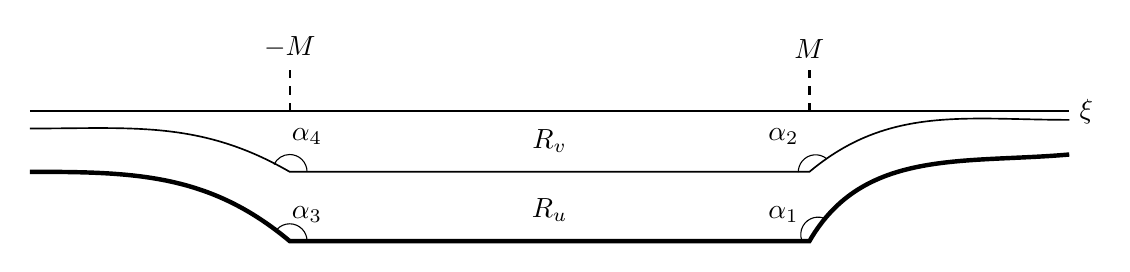
\begin{tikzpicture}[scale = 1.1]
\draw[thick](-6,0) -- (6,0) node[right] {$\xi$};
\draw [ultra thick] (-6,-0.7)to [out=0,in=140] (-3,-1.5) -- (3,-1.5) to [out=60,in=185] (6,-0.5);
\draw [semithick] (-6, -0.2) to [ out=0, in=150] (-3,-0.7) -- (3,-0.7)  to [out= 40, in=180] (6,-0.1);
\node[above] at (3,0.5) {$M$};
\draw[dashed] [thick] (3,0)-- (3,0.5);
\node[above] at (-3,0.5) {$-M$};
\draw[dashed] [thick] (-3,0)-- (-3,0.5);
\draw [thin] (-2.8,-1.5) arc [radius=0.2, start angle=0, end angle= 135];
\node[above] at (-2.8,-1.4) {$\alpha_3$};
\draw [thin] (-2.8,-0.7) arc [radius=0.2, start angle=0, end angle= 155];
\node[above] at (-2.8,-0.5) {$\alpha_4$};
\draw [thin] (3.2,-1.25) arc [radius=0.2, start angle=60, end angle= 200];
\node[above] at (2.7,-1.4) {$\alpha_1$};
\draw [thin] (3.2,-0.55) arc [radius=0.2, start angle=50, end angle= 180];
\node[above] at (2.7,-0.5) {$\alpha_2$};
\node[below] at (0,-0.9) {$R_u$};
\node[below] at (0,-0.1) {$R_v$};
%\node[below] at (0,-2.3) {Figure \ref{Figure ap}: $(R_u,R_v)$.};
\end{tikzpicture}
\caption{ $(R_u,R_v)$.}\label{Figure ap}
\end{center}
\end{figure}

We now define $(R_u,R_v)(\xi)$ as (see Figure 1)
\begin{equation*}
(R_u,R_v)(\xi):=\begin{cases}
(-\varepsilon_1e^{\lambda_1\xi},-\eta_1e^{\lambda_1\xi}),&\ \ \mbox{for}\ \ M\le\xi,\\
(-\varepsilon_1e^{\lambda_1 M},-\eta_1e^{\lambda_1 M}),&\ \ \mbox{for}\ \ -M\le\xi\le M,\\
(-\varepsilon_2(-\xi)^{1/2}[1-U_1(\xi)],-\eta_2(-\xi)^{1/2}V_1(\xi)),&\ \ \mbox{for}\ \ \xi\le -M,
\end{cases}
\end{equation*}
where $\lambda_{1}<\min\{\Lambda(c_1),\lambda_v^-(c_1)\}<0$ which is defined in Lemma \ref{lm: behavior around + infty}. Here $\varepsilon_{1,2}>0$ and $\eta_{1,2}>0$, will be determined later.

\noindent{\bf{Step 1}}
In this step, we consider $\xi\in[M,\infty)$. 
Recall that, $(U_1,V_1)$ is the minimal traveling wave satisfying \eqref{traveling wave c1}.
By some  straightforward computations,  we have
\begin{equation}\label{eq 1}
\begin{aligned}
N_5[\overline U,\underline V]=&(c_2-c_1)U'_1-(\lambda_1^2+c_2\lambda_1)R_u\\
&-R_u(1-2U_1+R_u-aV_1-aR_v)-aR_vU_1,
\end{aligned}
\end{equation}
and
\begin{equation}\label{eq 2}
\begin{aligned}
N_6[\overline U,\underline V] = &(c_2-c_1)V_1'+ (d\lambda_1^2+c_2\lambda_1)R_v+ rR_v(1-2V_1-R_v-U_1+R_u)\\
&-r\delta_0(V_1+R_v)(U_1-R_u).
\end{aligned}
\end{equation}

By Lemma \ref{lm: behavior around + infty}, there exists $C_1>0$ such that 
$$(c_2-c_1)U_1'\le -C_1(c_2-c_1)U_1\ \ \text{for all}\ \ \xi\in[M,\infty)$$
up to enlarging $M$ if necessary.
Then, from the definition of $(R_u,R_v)$ and $\lambda_{1}<\min\{\Lambda(c_1),\lambda_v^-(c_1)\}<0$, we find
$$-(\lambda_1^2+c_2\lambda_1)R_u=o(U_1),\ -R_u(1-2U_1+R_u-aV_1-aR_v)=o(U_1),\ -aR_vU_1=o(U_1).$$
Therefore, by setting  $\varepsilon_1>0$ and $\eta_1>0$ relatively small, from \eqref{eq 1}, we have $N_5[\overline U,\underline V]\le 0$ for all $\xi\in[M,\infty)$.


Next, we deal with the inequality of $N_6[W_u, W_v]$. Since $\lambda_{1}<\min\{\Lambda(c_1),\lambda_v^-(c_1)\}<0$, we have
$$ (d\lambda_1^2+c_2\lambda_1)R_v=o(1-V_1), rR_v(1-2V_1-R_v-U_1+R_u)=o(1-V_1).$$
From Lemma \ref{lm: behavior around + infty}, there exists $C_2>0$ such that 
$$(c_2-c_1)V'_1\ge C_2(c_2-c_1)(1-V_1).$$
By the asymptotic behavior of $U_1$ in Lemma \ref{lm: behavior around + infty}, we have
$$(c_2-c_1)V'_1-r\delta_0(V_1+R_v)(U_1-R_u)>0,$$
provided that $\delta_0$ is sufficiently small.
Then, we have $N_6[W_u,W_v]\geq0$
for $\xi\geq M$ for $\varepsilon_1$  and $\eta_1$ sufficiently small. 

\noindent{\bf{Step 2}}
In this step, we consider $\xi\in[-M,M]$. In this case, $(R_u,R_v)$ are constants. By the definition, $(R_u.R_v)$ is continuous on $\xi=M$. It is easy to verify that 
$$\lim_{\xi\to M^+}R'_u(\xi)>0=\lim_{\xi\to M^-}R'_u(\xi)\quad\text{and}\quad \lim_{\xi\to M^+}R'_v(\xi)>0=\lim_{\xi\to M^-}R'_v(\xi),$$
which implies $\angle \alpha_1,\angle \alpha_2<180^{\circ}$. 
By some straightforward computation, we have 
 \begin{equation*}
N_5[\overline U,\underline V]=(c_2-c_1)U'_1-R_u(1-2U_1+R_u-aV_1-aR_v)-aR_vU_1,
\end{equation*}
and
\begin{equation*}
N_6[\overline U,\underline V] = (c_2-c_1)V_1'+ rR_v(1-2V_1-R_v-U_1+R_u)-r\delta_0(V_1+R_v)(U_1-R_u).
\end{equation*}
Since $[-M,M]$ is a bounded interval, by decreasing $\varepsilon_1$, $\eta_1$ and $\delta_0$ if necessary, one has $N_5[\overline U,\underline V]\le 0$ and 
$N_6[\overline U,\underline V]\ge 0$ for $\xi\in[-M,M]$.

\noindent{\bf{Step 3}}
In this step, we consider $\xi\in(-\infty,-M]$. In this case, we have 
$$(R_u,R_v)=(-\varepsilon_2(-\xi)^{1/2}[1-U_1(\xi)],-\eta_2(-\xi)^{1/2}V_1(\xi)).$$  
We take  
$$\varepsilon_2=\frac{\varepsilon_1e^{\lambda_1 M}}{M^{1/2}(1-U_1(-M))}\quad\text{and}\quad\eta_2=\frac{\eta_1e^{\lambda_1 M}}{M^{1/2}V_1(-M)}$$
such that $(R_u.R_v)$ is continuous on $\xi=-M$. It is easy to verify that 
$$\lim_{\xi\to -M^+}R'_u(\xi)=0>\lim_{\xi\to -M^-}R'_u(\xi)\quad\text{and}\quad \lim_{\xi\to -M^+}R'_v(\xi)=0>\lim_{\xi\to M^-}R'_v(\xi),$$
which implies $\angle \alpha_3,\angle \alpha_4<180^{\circ}$. 

%By some straightforward computation, one has 

Note that, there exists $M_0>M$ sufficiently large such that $\overline U=1$ and $\underline V=0$ for all $\xi\in(-\infty,-M_0]$. 
From the definition of $(R_u,R_v)$, by modify $\varepsilon_1/\eta_1$, we may assume $\overline U(\xi)<1$, $\underline V(\xi)>0$ for all $\xi>-M_0$ and 
$\overline U(\xi)=1$, $\underline V(\xi)=0$ for all $\xi\in(-\infty,-M_0]$, which implies that
$$N_5[\overline U,\underline V]\le 0\ \ \text{and}\ \ N_6[\overline U,\underline V]\ge 0\ \ \text{for}\ \ \xi\in(-\infty,-M_0].$$

It suffices to consider $\xi\in[-M_0,-M]$. 
By $R_u,R_v<0$ in $[-M_0,-M]$ and $U'_1<0$, we have 
\begin{equation}\label{N3 inequalifty -infty}
\begin{aligned}
N_5[\overline U,\underline V]=&(c_2-c_1)U'_1+\varepsilon_2(-\xi)^{1/2}\Big(-U_1''-c_2U_1'-\frac{1}{4}(-\xi)^{-2}(1-U_1)+(-\xi)^{-1}U_1'\\&-\frac{c_2}{2}(-\xi)^{-1}(1-U_1)\Big)
-R_u(1-2U_1+R_u-a(V_1+R_v))-aU_1R_v\\
\leq&(c_2-c_1)(U'_1-\varepsilon_2(-\xi)^{1/2}U'_1)+\varepsilon_2(-\xi)^{1/2}\Big(U_1(1-U_1-aV_1)-\frac{c_2}{2}(-\xi)^{-1}(1-U_1)\Big)\\&-R_u(1-2U_1+R_u-a(V_1+R_v))-aU_1R_v.
\end{aligned}
\end{equation}

Note that,  $1-U_1\ge -R_u$ in $\xi\in[-M_0,-M]$ and $1-U_1=-R_u$ on $\xi=-M_0$.
By the asymptotic behavior in Lemma \ref{lem:AS-infty:b=1}, one has
$(1-U_1)'\ge -R'_u$, which implies 
$$(c_2-c_1)(U'_1-\varepsilon_2(-\xi)^{1/2}U'_1)\le -\frac{(c_2-c_1)}{2}(-\xi)^{-1}R_u$$


Then, by using 
$\varepsilon_2(-\xi)^{1/2}U_1(1-U_1)=-R_uU_1$, from \eqref{N3 inequalifty -infty} we have
\beaa
N_5[W_u,W_v]&\le&-R_uU_1-a\varepsilon_2(-\xi)^{1/2}U_1V_1+\frac{c_2}{2}(-\xi)^{-1}R_u-R_u(1-2U_1-aV_1)
\\
&&-R_u^2+aR_uR_v+a\varepsilon_2(-\xi)^{1/2}U_1V_1 -\frac{(c_2-c_1)}{2}(-\xi)^{-1}R_u\\
&=&\frac{c_1}{2}(-\xi)^{-1}R_u-R_u(1-U_1-aV_1)-R_u^2+aR_uR_v.
\eeaa

Denote that
\beaa
I_1:=\frac{c_1}{2}(-\xi)^{-1}R_u,\quad
I_2:=-R_u(1-U_1-aV_1),\quad
I_3:=-R_u^2+aR_uR_v.
\eeaa
By the equation satisfied by $U_1$,  $1-U_1-aV_1>0$ for all $\xi\leq -M$ (if necessary, we may choose $M$ larger). Therefore, 
\beaa
I_3=-R_u^2+aR_uR_v\leq R_u\varepsilon_2(-\xi)^{1/2}(1-U_1-aV_1)(\xi)<0\quad \mbox{for}\quad \xi\in[-M_0,-M].
\eeaa
Moreover, in view of Lemma~\ref{lm: behavior around - infty b=1}, we have
$I_2=o(I_1)$ as $\xi\to-\infty$.
Then, up to enlarging $M$ if necessary, we have $N_5[\overline U,\underline V]\le 0$ for $\xi\in[-M_0,-M]$.

On the other hand, by some straight computations, we have
\beaa
N_6[\overline U,\underline V]&=&d\Big(V_1''+\frac{\eta_2}{4}(-\xi)^{-2/3}V_1+\eta_2(-\xi)^{-1/2}V'_1-\eta_2(-\xi)^{1/2}V''_1\Big)\\
&&+c_2\Big(V_1'+\frac{\eta_2}{2}(-\xi)^{-1/2}V_1-\eta_2(-\xi)^{1/2}V'_1\Big)\\&&
+r(V_1+R_v)(1-V_1-R_v-(1+\delta_0)(U_1-R_u)).\\
&\geq& r\eta_2(-\xi)^{1/2}V_1\Big((\eta_2(-\xi)^{1/2}-1)(1-U_1-V_1)
+\frac{c_2}{2r}(-\xi)^{-1}\Big)\\
&&+(c_2-c_1)(V_1'-\eta_2(-\xi)^{1/2}V_1')-r(U_1-R_u)(V_1+R_v)\delta_0.
\eeaa

By Lemma \ref{lm: behavior around - infty b=1},  
up to enlarging $M$, we have 
$(\eta_2(-\xi)^{1/2}-1)(1-U_1-V_1)>0$ for $\xi\in[-M_0,-M]$. 
Since  $V_1\ge -R_v$ in $\xi\in[-M_0,-M]$ and $V_1=-R_v$ on $\xi=-M_0$, we have
$V_1'\ge -R'_v$, which implies 
$$(c_2-c_1)(V'_1-\eta_2(-\xi)^{1/2}V'_1)\ge -\frac{(c_2-c_1)}{2}(-\xi)^{-1}R_v.$$
Thus
$$N_6[\overline U,\underline V]\ge \frac{c_1}{2}(-\xi)^{-1}R_v-r(U_1-R_u)(V_1+R_v)\delta_0.$$
It follows that
$N_6[\overline U,\underline V]\ge 0$ for $\xi\in[-M_0,-M]$
for all small $\delta_0>0$.
Therefore,
the construction for Step 3 is finished.

Now we are equipped with a super-solution satisfying \eqref{def: super solution 2}. Let us consider the spreading speed of the solution of 
\begin{equation}\label{eq 2}
    \left\{\begin{aligned}\relax
    & u_t=u_{xx}+u(1-u-av) \\ 
        & v_t=dv_{xx}+rv(1-v-(1+\delta_0)u), 
    \end{aligned}\right.
\end{equation}
with initial datum $u_0(x)$ compactly supported and $v_0(x)\equiv 1$.  It is known that the spreading speed is strictly greater than $\bar c$. 

On the other hand, it is easy to check that $(\overline u, \underline v)(t,x):=(\overline U,\underline V)(x-c_2t-x_0)$ is a super-solution of \eqref{eq 2}. Moreover, by setting $x_0>0$ large, one has $\overline u(0,x)\ge u_0(x)$ and $\underline v(0,x)\le v_0(x)$. Then, by the comparison principle, the spreading speed is smaller than or equal to $c_2$, which contradicts $c_2<\bar c$. 
\end{proof}
By Claim \ref{claim 1 AP} and Claim \ref{claim 2 AP}, we can assert that $c^*_{LV}(1)$ is well defined and $c^*_{LV}(b)$ is continuous for all $b\in(0,+\infty)$. The proof of Proposition \ref{prop:existence-appendix} is complete.
\end{proof}



\subsection{Asymptotic behavior of traveling waves of \eqref{system} near $+\infty$}\label{subsec:Asymp behavior}
%\blue{I think we should remove this subsection and finish the introduction by the last subsection since this result in this subsection is not beneficial for the reader to understand our main result.}

\noindent

In this subsection, we provide the asymptotic behavior of $(U_c,V_c)$ near $\pm\infty$
for $0<a<1$ and $b>0$, where $(U_c,V_c)$ satisfies either \eqref{tw solution weak} or \eqref{tw solution weak} with speed $c$.
Some results are reported in \cite{MoritaTachibana2009}.
We further establish an implicit condition that determines the asymptotic behavior of the {\em pushed transition front} $U_{c_{LV}^*}$ at $+\infty$. Furthermore, the degenerate case $a=1$ and $b\neq 1$ is also discussed.



We transform \eqref{TW-appendix} into a 4-dimensional first-order system of ordinary differential equations by introducing the notation $P(\xi)=U'(\xi)$, $Q(\xi)=V'(\xi)$:
\begin{equation}\label{eq:4dim-flow}
    \left\{\begin{aligned}\relax
        &U'=P  &                    =:&F_1(U, P, V, Q), \\ 
        &P'=-cP-U(1-U-aV)&              =:&F_2(U, P, V, Q), \\ 
        &V'=Q        &          =:&F_3(U, P, V, Q), \\ 
        &Q'=-\frac{c}{d}Q-\frac{r}{d}V(1-bU-V)& =:&F_4(U, P, V, Q).
    \end{aligned}\right.
\end{equation}
We let $F(U, P, V, Q) = \big(F_1(U, P, V, Q),F_2(U, P, V, Q),F_3(U, P, V, Q), F_4(U, P, V, Q)\big)^T$ be the vector field corresponding to \eqref{eq:4dim-flow}. 
The Jacobian matrix of the vector field is
\begin{equation*}
    DF(U,P,V,Q) = \left(\begin{matrix}
        0 & 1 & 0 & 0 \\ 
        -1+2U+aV & -c & aU & 0 \\
        0 & 0 & 0 & 1 \\
        \frac{r}{d}bV & 0 & -\frac{r}{d}(1-bU-2V) & -\frac{c}{d} 
    \end{matrix}\right)
\end{equation*}

Next, we study the linearized problem in the neighborhood of the state $(U, P, V, Q)=(0, 0, 1, 0)$. The Jacobian matrix is 
\begin{equation}\label{eq:Jacobian-invaded}
    DF(0, 0, 1, 0) = \begin{pmatrix}
        0 & 1 & 0 & 0 \\ 
        -1+a & -c & 0 & 0 \\ 
        0 & 0 & 0 & 1 \\ 
        \frac{r}{d}b & 0 & \frac{r}{d} & \frac{-c}{d}
    \end{pmatrix}
\end{equation}
Since it is  block triangular it is easy to compute its characteristic polynomial $\chi_{+\infty}(X)$
\begin{equation}\label{kkkk}
    \chi_{+\infty}(X) = \big(X^2+cX+1-a\big)\left(X^2+\frac{c}{d}X-\frac{r}{d}\right).
\end{equation}
Therefore the spectrum of the matrix $ DF(0, 0, 1, 0)$ is 
\begin{equation*}
    \sigma_{+\infty} = \left\{\dfrac{-c\pm\sqrt{c^2+4(a-1)}}{2},\dfrac{-c\pm\sqrt{c^2+4rd}}{2d}\right\}. 
\end{equation*}
Notice that,  the equilibrium has a one-dimensional center space if $a=1$. 
The corresponding eigenelements are: \medskip

\noindent $\bullet$ if  $a<1$ and $c>2\sqrt{1-a}$,
\begin{equation*}
\begin{aligned}
    %\label{eq:eigs+inftyu-a>1}
    \lambda_{u}^{-}&:= \dfrac{-c-\sqrt{c^2+4(a-1)}}{2},\ \lambda_{u}^{+}:=\dfrac{-c+\sqrt{c^2+4(a-1)}}{2},\\
    \lambda_{v}^{-}&:= \dfrac{-c-\sqrt{c^2+4rd}}{2d},\ \lambda_{v}^{+}:= \dfrac{-c+\sqrt{c^2+4rd}}{2d},\\
    X^{-}_{u}&:=\left(1, \lambda_{u}^{-}, \frac{rb}{-r+c\lambda_{u}^{-}+d(\lambda_{u}^{-})^2}, \dfrac{\lambda_{u}^{-}rb}{-r+c\lambda_{u}^{-}+d(\lambda_{u}^{-})^2}\right)^T,  \\
    %\label{eq:eigs+inftyu+a>1}
   X^{+}_{u}&:= \left(1, \lambda_{u}^{+}, \dfrac{rb}{-r+c\lambda_{u}^{+}+d(\lambda_{u}^{+})^2}, \dfrac{\lambda_{u}^{+}rb}{-r+c\lambda_{u}^{+}+d(\lambda_{u}^{+})^2}\right)^T,   \\
    %\label{eq:eigs+inftyv-a>1}
    X^{-}_{v}&:=\left(0, 0, 1, \lambda_{v}^{-}\right), X^{+}_{v}:=\left( 0, 0, 1, \lambda_{v}^{+}\right),
    %\relax\label{eq:eigs+inftyv+a>1}
\end{aligned}
\end{equation*}
 provided $\lambda_{u}^{+}\neq \lambda_{v}^{+}$ and $\lambda_{u}^{+}\neq \lambda_{v}^{+}$.
If $\lambda_{u}^{\pm}=\lambda_{v}^{\pm}$, this eigenvalue is not associated with two distinct eigenvectors but with a plane spanned by $\mathcal{X}_{v}^{\pm}=X_{v}^{\pm}$ and 
\begin{equation*}%\label{eq:Xvpm-infty}
    \mathcal{X}_{u}^{\pm} = \left(\frac{2d\lambda_{v}^{\pm}+c}{rb}, \lambda_{v}^{\pm}\frac{2d\lambda_{v}^{\pm}+c}{rb}, 0, 1\right)^T, 
\end{equation*}
and the associated Jordan block in the $(\mathcal{X}_{v}^{\pm}, \mathcal{X}_{u}^{\pm})$ plane is 
\begin{equation*}
    \begin{pmatrix}
        \lambda_{v}^{\pm} & 1 \\ 0 & \lambda_{v}^{\pm}
    \end{pmatrix}.
\end{equation*}

\noindent $\bullet$ if $a=1$,
\begin{equation*}
\begin{aligned}
    %\label{eq:eigs+inftyu-a=1}
    \lambda_{u}^{-}&= -c,\ \lambda_{u}^{+}=0,\  \lambda_{v}^{-}= \dfrac{-c-\sqrt{c^2+4rd}}{2d},\ \lambda_{v}^{+}= \dfrac{-c+\sqrt{c^2+4rd}}{2d},\\
    X^{-}_{u}&=\left(1, \lambda_{u}^{-}, \dfrac{rb}{-r+c\lambda_{u}^{-}+d(\lambda_{u}^{-})^2}, \dfrac{\lambda_{u}^{-}rb}{-r+c\lambda_{u}^{-}+d(\lambda_{u}^{-})^2}\right)^T,   \\
    %\label{eq:eigs+inftyu+a=1}
     X^{+}_{u}&= \left(1, 0, -b, 0\right)^T,\ X^{-}_{v}=\left(0, 0, 1, \lambda_{v}^-\right), \  X^{+}_{v}=\left( 0, 0, 1, \lambda_{v}^+\right),
    %\label{eq:eigs+inftyv-a=1}
    %\relax\label{eq:eigs+inftyv+a=1}
\end{aligned}
\end{equation*}
provided $\lambda_{v}^{-}\neq \lambda_{u}^{-}=-c$. If $\lambda_{v}^{-}=\lambda_{u}^{-}=-c$, then this eigenvalue is not associated with two distinct eigenvectors but with a plane spanned by $\mathcal{X}_{v}^{\pm}=X_{v}^{\pm}$ and 
\begin{equation}\label{eq:Xupm+infty}
    \mathcal{X}_{u}^{\pm} = \left(\frac{2d\lambda_{v}^{\pm}+c}{rb}, \lambda_{v}^{\pm}\frac{2d\lambda_{v}^{\pm}+c}{rb}, 0, 1\right)^T.
\end{equation}
%and the associated Jordan block in the $(\mathcal{X}_{v}^{\pm}, \mathcal{X}_{u}^{\pm})$ plane is 
%\begin{equation*}
    %\begin{pmatrix}
        %\lambda_{v}^{\pm} & 1 \\ 0 & \lambda_{v}^{\pm}
    %\end{pmatrix}.
%\end{equation*}

\noindent $\bullet$ if  $a<1$ and $c\leq 2\sqrt{1-a}$, then the eigenvalues in \eqref{kkkk}  have an imaginary part and  should be replaced by 
\begin{equation*}
\begin{aligned}
    %\label{eq:eigs+inftyu-a<1}
    \lambda_{u}^{-}&= \dfrac{-c-i\sqrt{4(1-a)-c^2}}{2},\ \lambda_{u}^{+}=\dfrac{-c+i\sqrt{4(1-a)-c^2}}{2},\\
    X^{-}_{u}&=\left(1, \lambda_{u}^{-},\dfrac{rb}{-r+c\lambda_{u}^{-}+d(\lambda_{u}^{-})^2}, \dfrac{\lambda_{u}^{-}rb}{-r+c\lambda_{u}^{-}+d(\lambda_{u}^{-})^2}\right)^T,   \\
    %\label{eq:eigs+inftyu+a<1}
    X^{+}_{u}&:=\left(1, \lambda_{u}^{+}, \dfrac{rb}{-rb+c\lambda_{u}^{+}+d(\lambda_{u}^{+})^2}, \dfrac{\lambda_{u}^{+}rb}{-rb+c\lambda_{u}^{+}+d(\lambda_{u}^{+})^2}\right)^T.
\end{aligned} 
\end{equation*}
\medskip


A traveling wave solution to \eqref{TW-appendix} would approach $(0,1)$ when $x\to +\infty$, therefore our interest lies in the unstable manifold of \eqref{eq:4dim-flow}, that is the space tangent to the eigenvectors corresponding to positive eigenvalues, here $\lambda_{u}^{+} $ and $\lambda_{v}^{+}$. 
Note that, the center eigenvalue in $DF(0, 0, 1, 0)$ when $a=1$, it is not immediate to determine the asymptotic behavior of $(U, V)$. We prove the following. 
\begin{proposition}[Asymptotic behavior near $+\infty$, $a=1$]\label{prop:asym-invaded} 
Let $a=1$,  $b>1$ and $0<c<b$ be given. Let $(U,V)(\xi)$ be  solution to \eqref{TW-appendix} with speed $c>0$ and such that 
    \begin{equation*}
        \lim_{\xi\to+\infty} U(\xi) = 0 \text{ and } \lim_{\xi\to+\infty} V(\xi)=1.
    \end{equation*}
    Then, as $\xi\to +\infty$, we have
    \begin{equation*}%\label{eq:asym-invaded}
        \limsup_{\xi\to +\infty} \dfrac{\ln\big(\max(|U(\xi)|, |V(\xi)-1|)\big)}{\xi}<0.
    \end{equation*}
    More precisely, 
    \begin{enumerate}
        \item[(1)] If $\lambda_{v}^{-} > -c$ then
            \begin{equation*}
                U(\xi) = B_u e^{-c \xi}+o\left(e^{-c\xi}\right) \text{ and } V(\xi) = 1+A_ve^{\lambda_{v}^{-}\xi} + o\left(e^{\lambda_{v}^{-}\xi}\right)
            \end{equation*}
            for some $B_u>0$ and $A_v<0$. 
        \item[(2)] If $-c>\lambda_{v}^{-}$ then 
            \begin{equation*}
                 U(\xi) = A_u e^{-c\xi}+o\left(e^{-c\xi}\right) \text{ and } V(\xi) = 1+A_ve^{-c\xi} + o\left(e^{-c\xi}\right)
            \end{equation*}
            for some $A_u>0$ and $A_v<0$. 
        \item[(3)] If $-c=\lambda_{v}^{-}$, then 
            \begin{equation*}
                U(\xi) = B_ue^{\lambda_{v}^{-}\xi}+ o\big(e^{\lambda_{v}^{-}\xi}\big) \text{ and } V(\xi) = 1+(A_v-B_u \xi)e^{\lambda_{v}^{-}\xi}+ o\big(e^{\lambda_{v}^{-}\xi}\big), 
            \end{equation*}
            for some $B_u>0$ and $A_v\in\mathbb R$.
    \end{enumerate}
\end{proposition}
\begin{proof}
    The first part of the proof is devoted to show the exponential convergence of $(U, V)(\xi)$ to  $(0, 1)$ or, to be more precise, to show that the traveling wave cannot approach $(0, 1)$ through a center manifold of \eqref{eq:4dim-flow}.  

    We fix a neighborhood $\Omega\ni (1, 0, 0, 0)$ and a smooth cut-off $g(\xi)$ of the vector field in \eqref{eq:4dim-flow} such that $\Omega \subset B\big((1, 0, 0, 0)^T, 1\big) $ (the ball of radius 1) and 
    \begin{enumerate} 
        \item for each $ Z=(U, P, V, Q)\in \Omega$ the cut-off $g(Z)$ coincides with the vector field $F(Z)$ in \eqref{eq:4dim-flow}, 
        \item for each $ Z \not\in B(Z_0, 1)$ we have $g(Z)=0$.
    \end{enumerate}
    Since $Z(\xi):=(U(\xi), P(\xi), V(\xi), Q(\xi))^T$ converges to $Z_0:=(1, 0, 0, 0)^T$ there exists a $\xi_0\in\mathbb R$ with the property that 
    \begin{equation*}
        Z(\xi)\in \Omega \text{ for all } \xi\geq \xi_0.
    \end{equation*}
    Therefore for $\xi\geq \xi_0$, $Z(\xi)$ has to belong to the unique global center stable manifold associated with the equation 
    \begin{equation} \label{eq:cutoff}
        Z'(\xi)=g(Z(\xi)).
    \end{equation}
    By applying \cite[Theorem 5.17]{Van-89} to the equation $Z'(\xi)=g(Z(\xi))$ reduced to the center stable manifold (up to a local straightening), there exists an orbit $\tilde Z(z)\in M_c$ which belongs to the center manifold of \eqref{eq:cutoff}  and $\eta>0$ such that 
    \begin{equation}\label{eq:proofpropinvadeda=1-1}
        \sup_{\xi\geq \xi_0} e^{\eta \xi}\Vert Z(\xi) -\tilde Z(\xi)\Vert < +\infty
    \end{equation}
    for $\xi_0$ sufficiently large. 
    
    We implicitly made the assumption that the Lipschitz norm of $g$ is small so that the existence,  uniqueness, and smoothness theory for the center manifold of $g$ can be applied (we refer to \cite[Theorem 2.1]{Van-89} for the existence and uniqueness of the global center manifold, and to \cite[Theorem 3.1]{Van-89} for the smoothness of the center manifold). In particular, there exists a $C^2$ map $\psi$, 
    \begin{equation*}
        \psi:X_c\to X_h, \text{ where }  X_c = \text{span}(X_{u}^{+}) \text{ and }X_h = \text{span}(X_{u}^{-}, X_{v}^{-}, X_{v}^{+}),
    \end{equation*}
    such that $\psi(0)=0$, $D\psi(0\cdot X_{u}^{+}) = 0$ and 
    \begin{equation*}
        \tilde Z(\xi) =  Z_0 + \zeta(\xi) X_{u}^{+} + \psi\big(\zeta(\xi) X_{u}^{+}\big), 
    \end{equation*}
    where 
    \begin{equation*}
        \zeta(\xi):=\text{proj}_{X_{u}^{+}}(\tilde Z(\xi)-Z_0).
    \end{equation*}
    Since $F$ is $C^2$, we have 
    \begin{equation*}
        F(Z) = F(Z_0)+DF(Z_0)(Z-Z_0)+\frac{1}{2}D^2F(Z_0)(Z-Z_0)^2 + o\big(\Vert Z-Z_0\Vert^2\big), 
    \end{equation*}
    where $DF(Z_0)=DF\big((1, 0, 0, 0)^T\big) $ is given by \eqref{eq:Jacobian-invaded} and $D^2F(Z_0)(Z-Z_0)^2$ is given by the formula
    \begin{equation*}
        D^2F(Z_0)(Z-Z_0)^2 = \begin{pmatrix}
            (Z-Z_0)^T H_u(Z_0) (Z-Z_0) \\ 
            (Z-Z_0)^T H_p(Z_0) (Z-Z_0) \\ 
            (Z-Z_0)^T H_v(Z_0) (Z-Z_0) \\ 
            (Z-Z_0)^T H_q(Z_0) (Z-Z_0) 
        \end{pmatrix},
    \end{equation*}
    where $H_u$, $H_p$, $H_v$ and $H_q$ are the Hessian matrices of $F$ with respect to each component:
    \begin{align*}
        H_u\big((u, p, v, q)^T\big) &= 0_{M_4(\mathbb R)}, & H_p\big((u, p, v, q)^T\big) &= 
        \begin{pmatrix}
            2 & 0 & a & 0 \\
            0 & 0 & 0 & 0 \\
            a & 0 & 0 & 0 \\
            0 & 0 & 0 & 0 
        \end{pmatrix},\smallskip \\
        H_v\big((u, p, v, q)^T\big)& = 0_{M_4(\mathbb R)}, &\text{ and }
        H_q\big((u, p, v, q)^T\big) &= 
        \begin{pmatrix}
            0 & 0 & b\frac{r}{d} & 0 \\ 
            0 & 0 & 0 & 0 \\
            b\frac{r}{d} & 0 & 2\frac{r}{d} & 0 \\ 
            0 & 0 & 0 & 0
        \end{pmatrix}.
    \end{align*}
    Therefore  (recalling $\psi(Y)=o(Y)$)
    \begin{align*}
        \tilde Z'(\xi) & =  DF(Z_0)\bigg(\zeta(\xi) X_{u}^{+} + \psi\big(\zeta(\xi) X_{u}^{+}\big)\bigg) + \frac{1}{2} D^2F(Z_0)\bigg(\zeta(\xi) X_{u}^{+} + \psi\big(\zeta(\xi) X_{u}^{+}\big)\bigg)+  o\big(\zeta(\xi)^2\big) \\ 
        &=DF(Z_0)\psi\big(\zeta(\xi)X_{u}^{+}\big) + \frac{1}{2}D^2F(Z_0)\big(\zeta(\xi)X_{u}^{+}\big)^2+  o\big(\zeta(\xi)^2\big), 
    \end{align*}
    and on the other hand
    \begin{equation*}
       \tilde Z'(\xi) = \zeta'(\xi)\bigg(X_{u}^{+} + \psi'\big(X_{u}^{+}\zeta(\xi)\big)\bigg). 
    \end{equation*}
    We left-multiply by the left eigenvector of $DF(Z_0)$ associated with the eigenvalue $0$,
    \begin{equation*}   
        Y_{u}^{+} = 
        \begin{pmatrix}
            c & 1 & 0 & 0
        \end{pmatrix} ,
    \end{equation*}
    to find that
    \begin{gather*}
        \zeta'(\xi)\bigg(c-b + Y_{u}^{+}\psi'\big(\zeta(\xi)X_{u}^{+}\big)\bigg)= 0 + \frac{1}{2}Y_{u}^{+} D^2F(Z_0)\big(\zeta(\xi)X_{u}^{+}\big)^2+  o\big(\zeta(\xi)^2\big), \\ 
        \dfrac{\zeta'(\xi)}{\zeta(\xi)^2} = \frac{1}{c-b}\bigg(\frac{1}{2}Y_{u}^{+} D^2F(Z_0)\big(X_{u}^{+}\big)^2 + o(1)\bigg) = \frac{b-1}{b-c}+o(1), 
    \end{gather*}
    where $o(1)\to 0$ as $x\to+\infty$. Integrating between $\xi_1\geq \xi_0$ and $\xi\geq \xi_1$, we have therefore
    \begin{gather*}
        \frac{1}{\zeta(\xi_1)}-\frac{1}{\zeta(\xi)} = \dfrac{b-1}{b-c}(\xi-\xi_1)(1+o(1)),  \\
        \zeta(\xi) = \dfrac{\zeta(\xi_1)}{1-\dfrac{b-1}{b-c}\zeta(\xi_1)(\xi-\xi_1)(1+o_{\xi_1}(1))} . 
    \end{gather*}
    Thus $\zeta(\xi_1)\leq 0$ for $\xi_1$ sufficiently large, or else $\zeta(\xi)$ (and $Z(\xi)$) would leave $\Omega$ in finite time, which would be a contradiction. Suppose that $\zeta(\xi_1)<0$, then 
    \begin{gather*}
        \zeta(\xi) =\frac{c-b}{(b-1)(\xi-\xi_1)} \left(\frac{1}{1+o_{\xi_1}(1)+\frac{c-b}{(b-1)\zeta(\xi_1)(\xi-\xi_1)}}\right) . 
    \end{gather*}
    Recalling \eqref{eq:proofpropinvadeda=1-1} we have then
    \begin{align*}
        Z(\xi) &= \tilde Z(\xi)+O(e^{-\eta \xi}) = Z_0+\zeta(\xi) X_{u}^{+} + o(\zeta(\xi)) + O(e^{-\eta \xi}) \\
        &= Z_0+\zeta(\xi) X_{u}^{+} + o(\zeta(\xi)) ,
    \end{align*}
    in particular $U(\xi)<0$ for $x$ large, which is a contradiction. 
   

   We conclude that $\zeta(\xi_1)=0$, therefore  $\zeta(\xi)\equiv 0$ and recalling \eqref{eq:proofpropinvadeda=1-1}, 
    \begin{equation*}
        \limsup_{\xi\to +\infty} e^{\eta \xi}\max(|U(\xi)|, |U'(\xi)|, |V(\xi)-1|, |V'(\xi)|)=0. 
    \end{equation*}
    In particular $Z(\xi)$ converges to $ Z_0$ exponentially fast and the rate of convergence is a negative eigenvalue of $DF(Z_0)$ \cite[Chap. 13, Theorem 4.3 p.335]{CoddingtonLevison}. The asymptotic behavior of $U(\xi)$ and $V(\xi)$ can be proved by the same argument for the case $a\neq 1$. The proof for Proposition \ref{prop:asym-invaded} is complete.
\end{proof}
\begin{proposition}\label{prop decay rate a=1}
 If $c>b$ then we cannot determine the asymptotic behavior of $U(\xi)$ and $V(\xi)$ as simply. The reason is that, in the proof of Proposition \ref{prop:asym-invaded}, we cannot rule out that $Z(\xi)$ approaches $Z_0$ with a non-zero component on the center manifold ($\zeta(\xi)\neq 0$). In this case $U(\xi)$ and $V(\xi)$ could converge to the equilibrium algebraically fast.
\end{proposition}


%Let $(c,U,V)$ be a solution of the system (\ref{tw solution}).
%Hereafter, for simplicity, we write $(U_c,V_c)$ as $(U,V)$.
%To describe the asymptotic behavior of $(U,V)$ near $+\infty$,
Hereafter, we denote
\beaa
&&\lambda_u^{\pm}(c):=\frac{c\pm\sqrt{c^2-4(1-a)}}{2}>0,\\ &&\lambda_v^{+}(c):=\frac{c+\sqrt{c^2+4rd}}{2d}>0>\lambda_v^{-}(c):=\frac{c-\sqrt{c^2+4rd}}{2d}.
\eeaa
The asymptotic behavior of $(U,V)$ near $+\infty$ for $0<a<1$ and $b>1$ can be found in \cite{MoritaTachibana2009}.
Note that the conclusions presented in \cite{MoritaTachibana2009} are still applicable for $b>0$ since $b$ is not present in the linearization at the unstable equilibrium $(0,1)$. Therefore, we have the following result.


\begin{lemma}[\cite{MoritaTachibana2009}]\label{lm: behavior around + infty}
Assume that $0<a<1$ and $b>0$.
Let $(c,U,V)$ be a solution of the system (\ref{tw solution weak}).
Then there exist positive constants $l_{i=1,\cdots,8}$ such that the following hold:
\begin{itemize}
\item[(i)]
For $c>2\sqrt{1-a}$,
\beaa
&&\lim_{\xi\rightarrow+\infty}\frac{U(\xi)}{e^{-\Lambda(c)\xi}}=l_1,\\
&&\lim_{\xi\rightarrow+\infty}\frac{1-V(\xi)}{e^{-\Lambda(c)\xi}}=l_2\quad \mbox{if $\lambda_v^{+}(c)>\Lambda(c)$},\\
&&\lim_{\xi\rightarrow+\infty}\frac{1-V(\xi)}{\xi e^{-\lambda_v^{+}(c)\xi}}=l_3\quad
\mbox{if $\lambda_v^{+}(c)=\Lambda(c)$},\\
&&\lim_{\xi\rightarrow+\infty}\frac{1-V(\xi)}{e^{-\lambda_v^{+}(c)\xi}}=l_4\quad
\mbox{if $\lambda_v^{+}(c)<\Lambda(c)$},
\eeaa
where $\Lambda(c)\in\{\lambda_u^+(c),\lambda_u^-(c)\}$. %\red{for nonlinear case, can we determine the value of $\Lambda(c)$?}.
\item[(ii)]
For $c=2\sqrt{1-a}$,
\beaa
&&\lim_{\xi\rightarrow+\infty}\frac{U(\xi)}{\xi^{p} e^{-\Lambda(c)\xi}}=l_5,\\
&&\lim_{\xi\rightarrow+\infty}\frac{1-V(\xi)}{\xi^p e^{-\Lambda(c)\xi}}=l_6\quad \mbox{if $\lambda_v^{+}(c)>\Lambda(c)$},\\
&&\lim_{\xi\rightarrow+\infty}\frac{1-V(\xi)}{\xi^{p+1} e^{-\Lambda(c)\xi}}=l_7\quad
\mbox{if $\lambda_v^{+}(c)=\Lambda(c)$},\\
&&\lim_{\xi\rightarrow+\infty}\frac{1-V(\xi)}{ e^{-\lambda_v^{+}(c)\xi}}=l_8\quad
\mbox{if $\lambda_v^{+}(c)<\Lambda(c)$},
\eeaa
where  $\Lambda(c)=\lambda_u^{\pm}(c)=\sqrt{1-a}$ %=\lambda_u^-(c)$}
and  $p\in\{0,1\}$.
\end{itemize}
\end{lemma}


\begin{remark}\label{rk:DuWangZhou}
In Lemma~\ref{lm: behavior around + infty}, if $c=c_{LV}^*>2\sqrt{1-a}$ (pushed front case), then from \cite[Lemma~ 2.3]{DuWangZhou} we have $\Lambda(c)=\lambda_u^{+}(c)$. %If $c>c_{LV}^*>2\sqrt{1-a}$, we have $\Lambda(c)=\lambda_u^{+}(c)$.
\end{remark}


When $c=2\sqrt{1-a}$, it is not clear whether $p=0$ or $p=1$.
By applying a similar argument used in \cite{Guo Wu} that considered the discrete version of \eqref{system},
we can derive an implicit criterion for determining whether $p=0$ or $p=1$, which is given in the following proposition.



\begin{proposition}\label{prop: implicit cond}
Assume that $0<a<1$ and $b>0$.
Let $(c,U,V)$ be a solution of \eqref{tw solution weak} with
$c=2\sqrt{1-a}$ and
$p$ be given in (ii) of Lemma~\ref{lm: behavior around + infty}.
Then
\bea\label{cond-p}
 p=
\begin{cases}
1 & \quad \mbox{if and only if}\quad  \int_{-\infty}^{\infty}e^{\Lambda(c)\xi}U(\xi)[a(1-V(\xi))-U(\xi)]d\xi\neq0,\\
0 & \quad \mbox{if and only if}\quad  \int_{-\infty}^{\infty}e^{\Lambda(c)\xi}U(\xi)[a(1-V(\xi))-U(\xi)]d\xi=0,
\end{cases}
\eea
where $\Lambda(c)=\lambda_u^{\pm}(c)=\sqrt{1-a}$.
\end{proposition}


The proof of Proposition~\ref{prop: implicit cond} is based on
a modified version of Ikehara's Theorem, which is given as follows:

\begin{proposition}[see Proposition 2.3 in \cite{Carr Chmaj}]\label{prop:ikehara}
For a positive non-increasing function $U$, we define
\begin{eqnarray*}
\dps F(\lambda):=\int_0^{+\infty} e^{-\lambda\xi} U(\xi) d\xi,\quad
\mbox{$\lambda\in\mathbb{C}$ with ${\rm Re}\lambda<0$}.
\end{eqnarray*}
If $F$ can be written as
$F(\lambda)={H(\lambda)}/{(\lambda+\gamma)^{p+1}}$
for some constants $p>-1, \gamma>0$, and some analytic function $H$
in the strip $-\gamma\leq {\rm Re}\lambda<0$, then
\begin{eqnarray*}
\lim_{\xi\rightarrow +\infty}
\frac{U(\xi)}{{\xi}^{p}e^{-\gamma\xi}}=\frac{H(-\gamma)}{\Gamma(\gamma+1)}.
\end{eqnarray*}
\end{proposition}


\begin{proof}[Proof of Proposition~\ref{prop: implicit cond}]
In fact, by modifying the process used in \cite{Guo Wu}, we can prove Lemma~\ref{lm: behavior around + infty} and
\eqref{cond-p} independently; however, the proof is quite long.
Instead of giving detailed proof,
we simply assume that Lemma~\ref{lm: behavior around + infty} hold and derive
\eqref{cond-p} by using Proposition~\ref{prop:ikehara}.


Let us  define the bilateral Laplace transform of $U$ as
\beaa
\mathcal{L}(\lambda):=\int_{-\infty}^{+\infty}e^{-\lambda \xi}U(\xi) d\xi,
\eeaa
which is well-defined for $-\Lambda(c)<{\rm Re} \lambda<0$
(since we have assumed that Lemma~\ref{lm: behavior around + infty} holds).
Using the equation of $U$ and integration by parts several times, we have
\bea\label{Phi-eq}
\Phi(\lambda)\mathcal{L}(\lambda)+I(\lambda)=0,\quad -\Lambda(c)<{\rm Re} \lambda<0,
\eea
where
\beaa
\Phi(\lambda):=c\lambda+\lambda^2+1-a,\quad I(\lambda):=\int_{-\infty}^{\infty}e^{-\lambda \xi}U[a(1-V)-U](\xi)d\xi.
\eeaa
To apply Ikehara's Theorem, we
rewrite \eqref{Phi-eq} as
\beaa
F(\lambda):=\int_{0}^{+\infty}e^{-\lambda \xi}U(\xi) d\xi
=-\frac{I(\lambda)}{\Phi(\lambda)}-\int_{-\infty}^{0}e^{-\lambda \xi}U(\xi) d\xi,
\eeaa
as long as $\Phi(\lambda)$ does not vanish.
Also, we define
\bea\label{Ikehara-from}
H(\lambda):=Q(\lambda)-[\lambda+\Lambda(c)]^{p+1}\int_{-\infty}^{0}e^{-\lambda \xi}U(\xi) d\xi,
\eea
where $\Lambda(c)=\sqrt{1-a}$, $p\in\mathbb{N}\cup\{0\}$, and
\bea\label{Q-func}
Q(\lambda):=-\frac{I(\lambda)}{\Phi(\lambda)/[\lambda+\Lambda(c)]^{p+1}}.
\eea

We now prove that $H$ is analytic in the strip $S:=\{-\Lambda(c)\leq {\rm Re}\lambda<0\}$.
Since the second term on the right-hand side of \eqref{Ikehara-from} is always analytic for ${\rm Re}\lambda<0$,
it suffices to show that $Q$ is analytic in the strip $S$.
Since $\mathcal{L}$ is well-defined for $-\Lambda(c)< {\rm Re}\lambda<0$, we see that
$Q$ is analytic for $-\Lambda(c)< {\rm Re}\lambda<0$. Therefore, it suffices to prove the
analyticity of $Q$ on $\{{\rm Re}\lambda=-\Lambda(c)\}$.
For this, we claim that the only root of $\Phi(\lambda)=0$ is the real root $\lambda=-\Lambda(c)$.
To see this, let $\lambda=\alpha +\beta i$ for $\alpha,\beta\in\mathbb{R}$ and $i:=\sqrt{-1}$. If
$\Phi(\alpha +\beta i)=0$, then by simple calculations we see that $\beta=0$ and $\alpha=-\Lambda(c)$.
Therefore, from \eqref{Q-func} we see that $Q$ is analytic on $\{{\rm Re}\lambda=-\Lambda(c)\}$ and is also analytic in $S$. Then, Ikehara's Theorem can be applied to assert that
\beaa
\lim_{\xi\to+\infty}\frac{U(\xi)}{{\xi}^{p}e^{\Lambda(c)\xi}}=\frac{H(-\Lambda(c))}{\Gamma(\Lambda(c)+1)}=
\frac{Q(-\Lambda(c))}{\Gamma(\Lambda(c)+1)}.
\eeaa

Finally, we need to prove $Q(-\Lambda(c))\neq0$ by taking suitable $p$.
To do so, note that \eqref{Q-func} and the fact that $\Phi(\lambda)=0$ imply that $\lambda=-\Lambda(c)$.
We see that, if $I(-\Lambda(c))\neq0$, then $Q(-\Lambda(c))\neq0$ if and only if $p=1$.
On the other hand, when $I(-\Lambda(c))=0$, then $\lambda=-\Lambda(c)$ must be simple root of $I(\lambda)=0$. Otherwise,
we have $Q(-\Lambda(c))=0$ for any $p\in\mathbb{N}\cup\{0\}$, which contradicts
the conclusion (ii) of Lemma~\ref{lm: behavior around + infty}. Therefore, when $I(-\Lambda(c))=0$,
we have $Q(-\Lambda(c))\neq0$ if and only if $p=0$, so \eqref{cond-p} holds.
This completes the proof.
\end{proof}


\subsection{Asymptotic behavior of traveling waves of \eqref{system} near $-\infty$}\label{subsec:Asymp behavior -}
To describe the asymptotic behavior of $(U,V)$ near $-\infty$, we define
\beaa
&&\mu_{u}^{-}(c):=\frac{-c-\sqrt{c^2+4}}{2}<0<\mu_{u}^{+}(c):=\frac{-c+\sqrt{c^2+4}}{2},\\
&&\mu_v^{-}(c):=\frac{-c-\sqrt{c^2+4rd(b-1)}}{2d}<0<\mu_v^{+}(c):=\frac{-c+\sqrt{c^2+4rd(b-1)}}{2d}.
\eeaa

\begin{lemma}[\cite{MoritaTachibana2009}]\label{lem:AS-infty:b>1}
Assume that $0<a<1$ and $b>1$.
Let $(c,U,V)$ be a solution of the system (\ref{tw solution weak}). Then
there exist two positive constants $l_{i=9,\cdots,12}$ such that
\beaa
&& \lim_{\xi\rightarrow-\infty}\frac{V(\xi)}{e^{\mu_v^+(c)\xi}}=l_9,\\
&&\lim_{\xi\rightarrow-\infty}\frac{1-U(\xi)}{e^{\mu_v^+(c)\xi}}=l_{10}\quad \mbox{if $\mu_{u}^{+}(c)>\mu_v^+(c)$},\\
&&\lim_{\xi\rightarrow-\infty}\frac{1-U(\xi)}{|\xi|e^{\mu_v^+(c)\xi}}=l_{11}\quad
\mbox{if $\mu_{u}^{+}(c)=\mu_v^+(c)$},\\
&&\lim_{\xi\rightarrow-\infty}\frac{1-U(\xi)}{e^{\mu_u^+(c)\xi}}=l_{12}\quad \mbox{if $\mu_{u}^{+}(c)<\mu_v^+(c)$}.
\eeaa
\end{lemma}

\bigskip
\begin{lemma}\label{lem:AS-infty:b<1}
Assume that $0<a,b<1$.
Let $(c,U,V)$ be a solution of the system (\ref{tw solution weak}).
Then there exist two positive constants $l_{13}$ and $l_{14}$ such that
\beaa
\lim_{\xi\to-\infty}\frac{u^*-U(\xi)}{e^{\nu\xi}}=l_{13},\quad
\lim_{\xi\to-\infty}\frac{V(\xi)-v^*}{e^{\nu\xi}}=l_{14}
\eeaa
where
$\nu$ is the smallest positive zero of
\bea\label{chara-poly}
\rho(\lambda):=(\lambda^2+c\lambda-u^*)(d\lambda^2+c\lambda-rv^*)-rabu^*v^*.
\eea
\end{lemma}
\begin{proof}
Set
$g_u(\lambda):=\lambda^2+c\lambda-u^*$ and $g_v(\lambda):=d\lambda^2+c\lambda-rv^*$.
Then $g_u$ (resp., $g_v$) has two zeros $\mu^{u}_{\pm}$ (resp. $\mu^{v}_{\pm}$) with
$\mu^{u}_{-}<0< \mu^{u}_{+}$ (resp., $\mu^{v}_{-}<0< \mu^{v}_{+}$). More precisely, we have
\beaa
\mu^u_{\pm}=\frac{-c\pm\sqrt{c^2+4u^*}}{2},\quad \mu^v_{\pm}=\frac{-c\pm\sqrt{c^2+4drv^*}}{2d}.
\eeaa

Note that
$\rho(\lambda)=g_u(\lambda)g_v(\lambda)-rabu^*v^*$. Since $\rho(\pm\infty)=+\infty$,
$\rho(\mu^{u}_{\pm})<0$, $\rho(\mu^{v}_{\pm})<0$, and $\rho(0)=ru^*v^*(1-hk)>0$, we see that
$\rho$ has exactly four distinct real zeros $\lambda=\nu_i$ $(i=1,2,3,4)$, two negative and two positive zeros, such that
\beaa
\nu_4<\min\{\mu^{u}_{-},\mu^{v}_{-} \}\leq \max\{\mu^{u}_{-},\mu^{v}_{-} \}<\nu_3<0<\nu_2
<\min\{\mu^{u}_{+},\mu^{v}_{+} \}\leq \max\{\mu^{u}_{+},\mu^{v}_{+} \}<\nu_1.
\eeaa

%\red{It is better to change $(X_1,X_2,X_3,X_4)$ to $(U,P,V,Q)$ like (1.16) and that in Page 28
%Set $(X_1,X_2,X_3,X_4)(\xi)=(U,U',V,V')(\xi)$.
Set $P=U'$ and $Q=V'$.
Then from \eqref{system}, we have
\bea\label{X-sys}
\qquad U'= P, \ P'=-c P-U(1-U-a V),\ V'= Q,
\ Q'=-\frac{c}{d}Q-\frac{r}{d}V(1-V-bU).
\eea

Linearizing \eqref{X-sys} at $(U,P,V,Q)=(u^*,0,v^*,0)$ yields that ${\bf Y}'=J {\bf Y}$, where
${\bf Y}=(Y_1,Y_2,Y_3,Y_4)^T$ and
\beaa
J:=
\left(\begin{array}{cccc} 0 & 1 & 0 & 0\\
                       u^* & -c & au^* & 0\\
                       0 & 0 & 0 & 1 \\
                       -\frac{rb}{d}v^* & 0 & \frac{r}{d}v^* & -\frac{c}{d}
                       \end{array}\right).
\eeaa
Using cofactor expansions, one has ${\rm det}(J-\lambda I)=\rho(\lambda)$,
where $\rho(\lambda)$ is defined in \eqref{chara-poly}. Hence,
$J$ has four distinct real eigenvalues $\nu_4<\nu_3<0<\nu_2<\nu_1$.
By straightforward calculations, for each eigenvalue $\nu_i$, the corresponding eigenvector ${\bf w}_i$ is given by
\beaa%\label{eigenv}
{\bf w}_i:=\Big(1,\nu_i,\frac{g_u(\nu_i)}{au^*},\nu_i \frac{g_u(\nu_i)}{au^*}\Big)^T,\quad i=1,2,3,4.
\eeaa
Therefore, the general solution of ${\bf Y}'=J {\bf Y}$ with ${\bf Y}(-\infty)={\bf 0}$ is given by
${\bf Y}(\xi)=\sum_{i=1}^{2}K_i  e^{\nu_i\xi}{\bf w}_i$ for some constants $K_i\in\mathbb{R}$, $i=1,2$.
By standard ODE theory, as $\xi\to-\infty$,
\bea\label{expansion}
\left(\begin{array}{c} U(\xi)\\ U'(\xi) \\ V(\xi) \\V'(\xi) \end{array}\right)=
%\left(\begin{array}{c} X_1(\xi) \\ X_2(\xi) \\X_3(\xi)\\ X_4(\xi) \end{array}\right)=
\left(\begin{array}{c} u^*+K_1  e^{\nu_1\xi}+K_2  e^{\nu_2\xi} \\
                            K_1  \nu_1 e^{\nu_1\xi}+ K_2 \nu_2 e^{\nu_2\xi}\\
                         v^*+K_1 \frac{g_u(\nu_1)}{au^*}   e^{\nu_1\xi}+K_2 \frac{g_u(\nu_2)}{au^*}   e^{\nu_2\xi}\\
                              K_1 \nu_1\frac{g_u(\nu_1)}{au^*} e^{\nu_1\xi}+K_2 \nu_2\frac{g_u(\nu_2)}{au^*}   e^{\nu_2\xi}
                              \end{array}\right)+h.o.t.
\eea
Clearly, $K_1^2+K_2^2\neq0$. If $K_2=0$, then
$K_1\neq0$  and it follows from
\eqref{expansion} that 
$$U'(\xi)\sim K_1  \nu_1 e^{\nu_1\xi}\ \ \text{and}\ \ V'(\xi)\sim K_1 \nu_1\frac{g_1(\nu_1)}{au^*} e^{\nu_1\xi}\ \ \text{as}\ \ \xi\to-\infty.$$
Since $\nu_1>\max\{\mu^u_+, \mu^v_+\}$, we see that $g_1(\nu_1)>0$.
This implies that $U'$ and $V'$ have the same sign as $\xi\to -\infty$,
which is impossible since
$U'<0$ and $V'>0$ in $\mathbb{R}$. Therefore, we obtain $K_2\neq0$. Moreover,
we have $K_2<0$ due to the monotonicity of $U$ and $V$.
The proof is thus complete by taking $\nu=\nu_2$, $l_{13}=-K_2$ and $l_{14}=K_2 g_u(\nu_2)/au^*$.
\end{proof}




For the strong-weak competition case ($b>1$) (resp.,
the weak competition case ($b<1$)), Lemma \ref{lem:AS-infty:b>1} and Lemma~\ref{lem:AS-infty:b<1} show that $(U,V)(\xi)$ converges to $(1,0)$ (resp., $(u^*,v^*)$) exponentially as $\xi\to-\infty$. %Furthermore, such asymptotic behaviors played an important role in the construction of $(R_u,R_v)(\xi)$ near $-\infty$.
However, in the critical case ($b=1$), the convergence rates may be of polynomial orders due to the degeneracy of the principal eigenvalue.

We now apply the center manifold theory to establish the decay rate of $U$ and $V$ at $\xi=-\infty$ when $b=1$. Let $W(\xi)=1-U(\xi)$. Then by simple calculations, $(W,V)$ satisfies
\bea\label{WVsys-b=1}
\begin{cases}
W''+cW'-(1-W)(W-aV)=0,&\quad \xi\in\mathbb{R},\\
dV''+cV'+rV(W-V)=0&\quad \xi\in\mathbb{R},\\
(W, V)(-\infty)=(0,0), \quad(W,V)(+\infty)=(1,1)
\end{cases}
\eea
To reduce \eqref{WVsys-b=1} to first-order ODEs, we introduce
\beaa
X_1(\xi)=V(\xi),\quad X_2(\xi)=V'(\xi), \quad X_3(\xi)=W(\xi),\quad X_4(\xi)=W'(\xi).
\eeaa
Then $X:=(X_1,X_2,X_3,X_4)(\xi)$ satisfies
$X'=G(X)$, which is described as
\bea\label{X1X2X3X4sys}
\begin{cases}
\dps X_1'=X_2,&\quad \xi\in\mathbb{R},\\
\dps X_2'=-\frac{c}{d}X_2-\frac{r}{d}X_1(X_3-X_1),&\quad \xi\in\mathbb{R},\\
\dps X_3'=X_4,&\quad \xi\in\mathbb{R},\\
\dps X_4'=-cX_4+(1-X_3)(X_3-aX_1),&\quad \xi\in\mathbb{R},
\end{cases}
\eea
By linearizing \eqref{X1X2X3X4sys} at $(0,0,0,0)$, we obtain
${\bf Y}'=J {\bf Y}$, where
${\bf Y}=(Y_1,Y_2,Y_3,Y_4)^T$ and
\beaa
J:=
\left(\begin{array}{cccc} 0 & 1 & 0 & 0\\
0 & -\frac{c}{d} & 0 & 0\\
0 & 0 & 0 & 1 \\
-a & 0 & 1 & -c
\end{array}\right).
\eeaa
It is easy to calculate that $J$ has four eigenvalues
\beaa
\mu_1=0,\quad \mu_2=-\frac{c}{d}, \quad \mu_3:=\frac{-c-\sqrt{c^2+4}}{2}<0,\quad \mu_4:=\frac{-c+\sqrt{c^2+4}}{2}>0,
\eeaa
and the corresponding eigenvector $v_i$ with respect to $\mu_i$ is given by
\beaa
v_1=(1,0,a,0)^T,\ v_2=\Big(\omega, -\frac{c}{d}\omega,-ad,ac\Big)^T,\
v_3=(0,0,1,\mu_3)^T,\ v_4=(0,0,1,\mu_4)^T,
\eeaa
where
\bea\label{omega}
\omega:=-d-c^2+\frac{c^2}{d}.
\eea
%By linearizing \eqref{WVsys-b=1} at $(0,0)$, we have
%\beaa
%\begin{cases}
%\hat{W}''+c\hat{W}'-%\hat{W}+a\hat{V}=0,&\quad %\xi\in\mathbb{R},\\
%d\hat{V}''+c\hat{V}'=0&\quad \xi\in\mathbb{R},
%\end{cases}
%\eeaa
To reduce \eqref{X1X2X3X4sys} into the normal form, we set $Z=Q^{-1}X$, where $Z:=(Z_1,Z_2,Z_3,Z_4)^T$ and
$Q:=(v_1\ v_2\ v_3\ v_4)\in \mathbb{R}^{4\times 4}$.
By some tedious computations, we have
\bea\label{X-Z}
\begin{cases}
X_1=Z_1+\omega Z_2,&\quad X_2=-\frac{c}{d}\omega Z_2,\\
X_3=aZ_1-adZ_2+Z_3+Z_4,&\quad X_4=acZ_2+\mu_3Z_3+\mu_4 Z_4,
\end{cases}
\eea
and
\bea\label{Q-1}
Q^{-1}:=
\left(\begin{array}{cccc}
1 & \frac{d}{c} & 0 & 0\\
0 & -\frac{d}{c\omega} & 0 & 0\\
\frac{a\mu_4}{\mu_3-\mu_4} & \frac{da(c+\omega\mu_4 +d\mu_4)}{\omega c (\mu_3-\mu_4)} & -\frac{\mu_4}{\mu_3-\mu_4} & \frac{1}{\mu_3-\mu_4} \\
-\frac{a\mu_3}{\mu_3-\mu_4} &
-\frac{da(c+\omega\mu_3 +d\mu_3)}{\omega c (\mu_3-\mu_4)} & \frac{\mu_3}{\mu_3-\mu_4} & -\frac{1}{\mu_3-\mu_4}
\end{array}\right),
\eea
where $\omega$ is defined in \eqref{omega}.
By \eqref{X1X2X3X4sys}, \eqref{X-Z} and \eqref{Q-1}, some tedious computations yield that
\bea\label{Zsys}
\begin{cases}
Z_1'= g_1(Z),\\
Z_2'=-\frac{c}{d}Z_2+g_2(Z),\\
Z_3'=\mu_3Z_3+g_3(Z),\\
Z_4'=\mu_4Z_4+g_4(Z),
\end{cases}
\eea
where
\beaa
&&g_1(Z):=-\frac{r}{c}(Z_1+\omega Z_2)h_1(Z),\quad g_2(Z):=\frac{r}{\omega c}(Z_1+\omega Z_2)h_1(Z),\\
%&&g_3(Z):=\omega\Big[-q_{31}\frac{c}{d}+q_{32}\frac{c^2}{d^2}\Big]Z_2-q_{32}\frac{r}{d}(Z_1+\omega Z_2)h_1(Z)+q_{33}[acZ_2+\mu_4 Z_4]\\
%&&\qquad+q_{34}\Big\{-ac^2Z_2-c\mu_4Z_4+(1+h_2(Z))[-(a\omega+ad)Z_2+Z_4]+h_2(Z)Z_3\Big\},\\
&&g_3(Z):=-q_{32}\frac{r}{d}(Z_1+\omega Z_2)h_1(Z)+q_{34}h_2(z)h_3(z),\\
%&&g_4(Z):=\omega\Big[-q_{41}\frac{c}{d}+q_{42}\frac{c^2}{d^2}\Big]Z_2-q_{42}\frac{r}{d}(Z_1+\omega Z_2)h_1(Z)+q_{43}[acZ_2+\mu_3 Z_3]\\
%&&\qquad+q_{44}\Big\{-ac^2Z_2-c\mu_3Z_3+(1+h_2(Z))[-(a\omega-ad)Z_2+Z_3]+h_2(Z)Z_4\Big\},\\
&&g_4(Z):=-q_{42}\frac{r}{d}(Z_1+\omega Z_2)h_1(Z)+q_{44}h_2(z)h_3(z),\\
&&h_1(Z):=(a-1)Z_1-(\omega+ad)Z_2+Z_3+Z_4,\\
%&&h_2(Z):=-aZ_1+adZ_2-Z_3-Z_4.
&&h_2(Z):=aZ_1-adZ_2+Z_3+Z_4,\\
&&h_3(Z):=a(\omega+d)Z_2-Z_3-Z_4.\\
\eeaa
Here $q_{ij}$ is defined as the $i,j$ entry of the matrix $Q^{-1}$.
Note from the definition of $g_i$ and $h_i$, %with more detailed computations (using $q_{33}=-\mu_4q_{34}$, $q_{43}=-\mu_3 q_{44}$, $\mu_3+\mu_4=c$ and $\mu_3\mu_4=-1$),
we see that $g_i$ does have no linear term of $Z_i$ for $i=1,2,3,4$, and thus
\beaa
g_i({\bf0})=0,\quad Dg_i({\bf0})={\bf0},\quad i=1,2,3,4.
\eeaa
Therefore, we can apply the center manifold theory (see \cite[Chapter 18]{Wiggins}) to conclude that there exists a one-dimensional center manifold for \eqref{Zsys}, and $Z_i$, $i=2,3,4$ can be represented by a smooth function $Z_i=H_i(Z_1)$, $i=2,3,4$, for small $Z_1$.
We assume that
\beaa
H_i(Z_1)=C_iZ_i^2+o(|Z_1|^2),\quad i=2,3,4,
\eeaa
for some $C_i\in\mathbb{R}$. Indeed, $C_i$ is determined such that
\bea
&&H_2'(Z_1)g_1(Z)-\Big[-\frac{c}{d}Z_2+g_2(Z)\Big]=o(|Z_1|^2),\label{H2-eq}\\
&&H_3'(Z_1)g_1(Z)-(\mu_3Z_3+g_3(Z))=o(|Z_1|^2),\label{H3-eq}\\
&&H_4'(Z_1)g_1(Z)-(\mu_4Z_4+g_4(Z))=o(|Z_1|^2).\label{H4-eq}
\eea
By comparing the coefficients in front of $Z_1^2$ on the both sides of \eqref{H2-eq},
we need $C_2=-\frac{rd}{\omega c^2}(1-a)$.
Also, from \eqref{H3-eq} and \eqref{H4-eq},  with some tedious computations, we see that $C_3=C_4=0$.
Moreover, the flow on the center manifold is defined by
\beaa
Z_1'=g_1(Z_1,H_2(Z_1),H_3(Z_1),H_4(Z_1))=\frac{r}{c}(1-a)Z_1^2+o(|Z_1|^2),
\eeaa
for sufficiently small $Z_1(\xi)$,
which implies that
\beaa
Z_1(\xi)=-\frac{c}{r(1-a)}\xi^{-1}+o(|\xi|^{-1})\quad \mbox{as $\xi\to-\infty$}.
\eeaa
Therefore, the center manifold theory yields that if $0<Z_1(\xi)\ll1$, we have
\beaa
Z_1(\xi)\sim -\frac{c}{r(1-a)}\xi^{-1},\quad
Z_2(\xi)\sim-\frac{d}{r\omega(1-a)}\xi^{-2}\quad
\mbox{as $\xi\to-\infty$.}
\eeaa
Therefore,
in view of \eqref{X-Z} and the definition of $X_i$,
together with the fact that $0<U,V<1$ in $\mathbb{R}$,
we see that there exists  $l_{15}>0$ such that
\bea\label{AS-infty:b=1}
\lim_{\xi\to-\infty}\frac{V(\xi)}{\xi^{-1}}=l_{15},\quad \lim_{\xi\to-\infty}\frac{1-U(\xi)}{\xi^{-1}}=a l_{15},
\eea
%\red{or there exists  $l_{16}>0$,
%\bea\label{AS-incorrect}
%\lim_{\xi\to-\infty}\frac{1-U(\xi)}{e^{\mu_4\xi}}=l_{16},
%\eea
%since we have a one-dimensional manifold on which the solution decays to zero
%exponentially as $\xi\to-\infty$.
%If \eqref{AS-incorrect} holds, we have $V\equiv 0$, which contradicts the fact $0<V<1$, so we have \eqref{AS-infty:b=1}. I don't know the reason %why we get \eqref{AS-incorrect} from \eqref{X-Z}.}
Furthermore, it holds that
\bea\label{AS-infty2:b=1}
\lim_{\xi\to-\infty}\frac{1-U(\xi)}{V(\xi)}=a<1.
\eea
Combining \eqref{AS-infty:b=1} and \eqref{AS-infty2:b=1}, we have the following result.


\begin{lemma}\label{lem:AS-infty:b=1}
Assume that $0<a<1$ and $b=1$.
Let $(c,U,V)$ be a solution of the system (\ref{tw solution weak}).
Then there exist two positive constants $l_{15}$ such that
\beaa
\lim_{\xi\to-\infty}\frac{V(\xi)}{\xi^{-1}}=l_{15},\quad \lim_{\xi\to-\infty}\frac{1-U(\xi)}{\xi^{-1}}=a l_{15}, \quad \lim_{\xi\to-\infty}\frac{1-U(\xi)}{V(\xi)}=a<1.
\eeaa
\end{lemma}

%Therefore, to describe the asymptotic behavior of $(U_*,V_*)$ near $-\infty$ for the case $b=1$, we define
%\bea\label{def of tau u v}
%1-U_*(\xi)\approx \tau_u(\xi)\quad\text{and}\quad V_*(\xi)\approx \tau_v(\xi)\quad\text{as}\quad\xi\to-\infty.
%\eea
%Then, by linearization of \eqref{tw solution} at $(u,v)=(1,0)$, we have
%\begin{equation}\label{system tau u v}
%\begin{cases}
%\tau''_u+c^*\tau'_u-\tau_u+a\tau_v=0,\\
%d\tau''_v+c^*\tau'_v-r(b-1)\tau_v+r\tau_v(b\tau_u-%\tau_v)=0.
%\end{cases}
%\end{equation}
%It is important to keep the term $r\tau_v(\tau_u-\tau_v)$ in the equation of $\tau_v$ for the case $b=1$.
%By comparing the order of both sides of the equations, $(\tau_u,\tau_v)(\xi)$ can not be exponential decay.

Hence, we immediately obtain a Lemma as follows:

Thanks to Lemma~\ref{lem:AS-infty:b>1}, Lemma~\ref{lem:AS-infty:b<1} and Lemma~\ref{lem:AS-infty:b=1}, we immediately obtain

\begin{corollary}\label{lm: behavior around - infty b=1}
Assume that $0<a<1$ and $b>0$.
Let $(U,V)$ be a solution of the system (\ref{tw solution weak}) with speed $c$. Then it holds that
\beaa
1-U(\xi)-aV(\xi)=o(|\xi|^{-1}).
\eeaa
In particular, for the case $b=1$,
%%we have $\tau_u(\xi)=O(|\xi|^{-1})$ and %$\tau_v(\xi)=O(|\xi|^{-1})$. Moreover,
there exists $\xi_0$ near $-\infty$ such that $(1-U-V)(\xi)< 0$ for all $\xi\in(-\infty,\xi_0]$.
\end{corollary}

%\subsection{Asymptotic behavior of traveling waves of \eqref{nonlocal equation} near $\pm\infty$}\label{subsec:Asymp behavior}
%In this subsection, we provide the asymptotic behavior of $U_c$ near $\pm\infty$, where $U_c$ satisfies \eqref{scalar nonlocal tw-parameter s} with speed $c\ge c^*_0$ defined as \eqref{formula of c_NL}. Hereafter, for simplicity, we write $U_c$ as $U$.
%Some results are reported in \cite{Carr Chmaj,Coville}.
%We further establish an implicit condition that determines the asymptotic behavior of the {\em pushed transition front} $U_{c_{LV}^*}$ at $+\infty$.

%Let $(c,U,V)$ be a solution of the system (\ref{tw solution}).
%To describe the asymptotic behavior of $U$ near $+\infty$,
%we define
%\beaa
%g(\mu)=\frac{1}{\mu}\Big(\int_{\mathbb{R}}J(y)e^{\mu y}dy+f'(0)-1\Big).
%\eeaa
%Notice that, this function is positive for all

%\beaa
%&&\lambda_u^{\pm}(c):=\frac{-c\pm\sqrt{c^2-4(1-a)}}{2}<0,\\ &&\lambda_v^{-}(c):=\frac{-c-\sqrt{c^2+4rd}}{2d}<0<\lambda_v^{+}(c):=\frac{-c+\sqrt{c^2+4rd}}{2d}.
%\eeaa

%The asymptotic behavior of $(U,V)$ near $+\infty$ for $0<a<1$ and $b>1$ can be found in \cite{MoritaTachibana2009}.
%Note that the conclusions presented in \cite{MoritaTachibana2009} are still applicable for $b>0$ since $b$ is not present in the linearization at the unstable equilibrium $(0,1)$. Therefore, we have the following result.



\bigskip

\noindent{\bf Acknowledgement.}
Maolin Zhou is supported by the National Key Research and Development Program of China (2021YFA1002400).
Chang-Hong Wu is supported by the Ministry of Science and Technology of Taiwan.
Dongyuan Xiao is supported by the LabEx {\it Solutions Num\'{e}riques, Mat\'{e}rielles et Mod\'{e}lisation pour lEnvironnement et le Vivant} (NUMEV) of the University of Montpellier.

\begin{thebibliography}{20}% Replace 9 by 99 if 10 or more references
%
% Please note the use of "\and" between author names below
%
\bibitem{Alfaro Xiao}
{M. Alfaro and D. Xiao},
Lotka-Volterra competition-diffusion system: the critical case, Commun. Partial Differ. Equ., 48:2(2023), 182-208.

\bibitem{Alhasanat Ou2019-1}
{A. Alhasanat and C. Ou}, On a conjecture raised by Yuzo Hosono,
 J. Dyn. Diff. Equat., 31 (2019), 287-304.

\bibitem{Alhasanat Ou2019}
{A. Alhasanat and C. Ou}, Minimal-speed selection of traveling waves to the Lotka-Volterra
competition model, J. Differ. Equ. 266 (2019), 7357-7378.


%\bibitem{Alhasanat Ou2020}
%{A. Alhasanat, C. Ou}, On the conjecture for the pushed wavefront to the diffusive Lotka-Volterra competition model.
%J Math Biol. 80 (2020), 1413–1422.



\bibitem{Aronson Weinberger}
{D. G. Aronson and H. F. Weinberger},
Multidimensional nonlinear diffusion arising
in population genetics,
Adv. Math., 30 (1978), 33--76.

%\bibitem{log delay 1}
%{M. D. Bramson},
%Maximal displacement of branching Brownian motion, Comm. Pure Appl. Math., 31 (1978), 531--581.

%\bibitem{log delay 2}
%{M. D. Bramson},
%Convergence of solutions of the Kolmogorov equation to travelling waves, Mem. Amer. Math. Soc., 44, 1983.

\bibitem{Benguria Depassier1994}
{R. D. Benguria and M. C. Depassier},
Validity of the linear speed selection mechanism for fronts of the nonlinear diffusion equation,
Phys. Rev. Lett. 73 (1994), 2272-2274.

\bibitem{Benguria Depassier1996}
{R. D. Benguria and M. C. Depassier},
Speed of fronts of the reaction-diffusion equation,
Phys. Rev. Lett. 77 (1996), 1171-1173.


%\bibitem{Berestycki Hamel2007}
%{H. Berestycki, F. Hamel},
%Generalized travelling waves for reaction-diffusion equations, Perspectives in Nonlinear Partial Differential Equations, Contemporary Mathematics, American Mathematical Society, Providence, R.I., (2007), pp 101-123.

\bibitem{Berestycki Hamel2012}
{H. Berestycki and F. Hamel}, Generalized transition waves and their properties,
Commun. Pure Appl. Math. 65 (2012), 592-648.

\bibitem{Bonnefon Coville Garnier Roques2014}
{O. Bonnefon, J. Coville, J. Garnier, and L. Roques}, Inside dynamics of solutions of integro-differential equations, Discrete Contin. Dyn. Syst. B 19 (2014), 3057-3085.


\bibitem{Bosch Metz Diekmann}
{F. van den Bosch, J.A.J. Metz, and O. Diekmann},  
The velocity of spatial population expansion, J. Math. Biol., 28 (1990), 529–565.


 \bibitem{Carr Chmaj}
{J. Carr and A. Chmaj},
Uniqueness of travelling waves for nonlocal monostable equations,
Proc. Amer. Math. Soc. 132 (2004), 2433-2439.


\bibitem{Carrere}
{C. Carrere}, Spreading speeds for a two-species competition-diffusion system. J. Differential Equations, 264
(2018), 2133--2156.

 \bibitem{Chen Fu Guo}
 {X. Chen, S.-C. Fu, and J.-S. Guo},
 Uniqueness and asymptotics of traveling waves of monostable dynamics on lattices, SIAM J. Math. Anal. 38 (2006), 233–258.

 \bibitem{CoddingtonLevison} {E. A. Coddington and N. Levinson}, Theory
of Ordinary Differential Equations, McGraw-Hill, New York, 1955.

\bibitem{Coville}
{J. Coville, J. Dávila, and S. Martínez},
Nonlocal anisotropic dispersal with monostable nonlinearity,
J. Diff. Eqns.,
12 (2008), 3080-3118.

\bibitem{Coville Dupaigne}
J. Coville and L. Dupaigne,
Propagation speed of travelling fronts in non local reaction–diffusion equations,
Nonlinear Analysis: Theory, Methods \& Applications, 60(2005), 797-819.

\bibitem{DuWangZhou} {Y. Du, M.X. Wang, and M. Zhou}, Semi-wave and spreading speed for the diffusive competition model with a free boundary, J. Math. Pures Appl. 107 (2017), 253--287.

\bibitem{Du Li Zhou}
{Y. Du, F. Li, and  M. Zhou},
Semi-wave and spreading speed of the nonlocal Fisher-KPP equation with free boundaries,
Journal de Mathématiques Pures et Appliquées, 154 (2021), 30-66.




% \bibitem{Conley Gardner 1984}
%{C. Conley, R. Gardner},
%An application of the generalized Morse index to traveling wave solutions of a competitive reaction diffusion model,
%Indiana Univ. math. J., 33 (1984), 319--343.

%\bibitem{Ducrot Giletti Matano}
%{A. Ducrot, T. Giletti and H. Matano},
%Spreading speeds for multidimensional reaction-diffusion systems of the prey-predator type, Calc. Var. Partial Differential Equations, 58 (2019), Paper No. 137, 34 pp.

\bibitem{Fife1973}
{P. C. Fife}, Semilinear elliptic boundary value problems with small parameters,
Arch. Rat. and Mech. Anal., 52 (1973), 205--232.

\bibitem{Fife1976}
{P. C. Fife}, Boundary and interior transition layer phenomena for pairs of second-order differential equations, J. Math. Anal. Appl., 54 (1976), 497--521.

%\bibitem{Fife1977}
%{P. C. Fife}, Asymptotic analysis of reaction-diffusion wave fronts, Rocky Mountain
%J . Math., 7 (1977), 389--415.

\bibitem{Fife McLeod1977}
{P. C. Fife and J. B. McLeod}, The approach of solutions of nonlinear diffusion equations to travelling front solutions,
 Arch. Ration. Mech. Anal., 65 (1977), 335--361.

\bibitem{Fisher}
{R. A. Fisher},
The wave of advance of advantageous genes,
Ann. Eugen., 7 (1937), 335--369.

%\bibitem{Gardner}
%{R.A. Gardner},
%Existence and stability of traveling wave solutions of competition models: a degree theoretic,
%J. Differential Equations, 44 (1982), 343--364.

\bibitem{Gardner et al 2012}
{J. Garnier, T. Giletti, F. Hamel, and L. Roques}, Inside dynamics of pulled and pushed fronts,
J Math Pures Appl, 98 (2012), 428-449.


%\bibitem{Girardin}
%{L. Girardin},
%The effect of random dispersal on competitive exclusion-a review, Mathematical Biosciences, 318 (2019), 108271.

\bibitem{Girardin Lam}
{L. Girardin, K.-Y. Lam},
Invasion of an empty habitat by two competitors: spreading properties of monostable
two-species competition-diffusion systems, Proc. Lond. Math. Soc., 119 (2019), 1279--1335.

\bibitem{Girardin Nadin}
{L. Girardin and G. Nadin},
Travelling waves for diffusive and strongly competitive systems: relative motility and
invasion speed, European J. Appl. Math., 26 (2015), 521--534.

\bibitem{Guo Liang}
{J.-S. Guo and X. Liang},
The minimal speed of traveling fronts for the Lotka-Volterra competition system,
J. Dynamics Diff. Equations, 23 (2011), 353--363.

\bibitem{Guo Lin}
{J.-S. Guo and Y.-C. Lin}, The sign of the wave speed for the Lotka-Volterra competition-diffusion system, Comm. Pure Appl. Anal., 12 (2013), 2083--2090.


\bibitem{Guo Wu}
{J.-S. Guo and C.-H. Wu},
Traveling wave front for a two-component lattice dynamical system
arising in competition models, J. Diff. Eqns.,  252 (2012), 4357--4391.

\bibitem{Hadeler Rothe}
{K. Hadeler and F. Rothe},
Travelling fronts in nonlinear diffusion equations, J. Math.
Biol. 2 (1975), 251-263.


%\bibitem{Hamel Roques} {F. Hamel, L. Roques},
%Uniqueness and stability properties of monostable pulsating fronts, J. Eur. Math. Soc.
%13 (2011), 345–390.


%\bibitem{log delay 3}
%{F. Hamel, J. Nolen, J. M. Roquejoffre and L. Ryzhik},
%A short proof of the logarithmic Bramson correction in Fisher-KPP equations, Netw. Heterog. Media., 8 (2013), 261--289.

\bibitem{Holzer Scheel 2012}
{M. Holzer and A. Scheel}, A slow pushed front in a Lotka-Volterra competition model, Nonlinearity
25 (2012), 2151.

\bibitem{Hosono 1995}
{Y. Hosono}, Traveling waves for diffusive Lotka-Volterra competition model ii: a geometric approach.
Forma 10 (1995), 235-257.

\bibitem{Hosono 1998}
{Y. Hosono}, The minimal speed of traveling fronts for a diffusive Lotka Volterra competition
model, Bull. Math. Biol., 60 (1998), 435-448.

\bibitem{Hosono 2003}
{Y. Hosono}, Traveling waves for a diffusive Lotka-Volterra competition model I: singular perturbations.
Disc Cont Dyn Systems B 3 (2003), 79-95.

\bibitem{Hosono Mimura 1982}
{Y. Hosono and M. Mimura}, Singular perturbation approach to traveling waves in competing and diffusing species models. Journal of Mathematics of Kyoto University 22 (1982), 435-461.

\bibitem{Huang2010}
{W. Huang}, Problem on minimum wave speed for a Lotka-Volterra reaction-diffusion competition model,
J. Dyn. Diff. Equat., 22 (2010), 285-297.

\bibitem{HuangHan2011}
{W. Huang and M. Han}, Non-linear determinacy of minimum wave speed for a Lotka-Volterra competition
model, J. Diff. Eqns., 251 (2011), 1549-1561.

\bibitem{Ito1985}
{M. Ito}, A remark onsin gular perturbation methods, Hiroshima Math. J. 14 (1984), 619–629.
%\bibitem{Iida Lui Ninomiya}
%{M. Iida, R. Lui and H. Ninomiya},
%Stacked fronts for cooperative systems with equal diffusion coefficients, SIAM J. Math. Anal., 43 (2011), 1369--1389.

\bibitem{Kan-On}
{Y. Kan-On},
Parameter dependence of propagation speed of travelling waves for competition-diffusion equations,
SIAM J. Math. Anal., 26 (1995), 340--363.

%\bibitem{Kan-On Fang}
%{Y. Kan-On, Q. Fang}, Stability of monotone travelling waves for competition-diffusion equations, Japan J. Indust. Appl. %Math., 13 (1996), 343--349.


\bibitem{Kan-on1997}
{Y. Kan-on}, Fisher wave fronts for the Lotka-Volterra competition model with diffusion, Nonlinear Anal., 28 (1997), 145--164.


\bibitem{KPP}
{A. N. Kolmogorov, I. G. Petrovskii, and N. S. Piskunov},
A study of the equation of diffusion with increase in the quantity of matter, and its application to a biological problem,
Bull. Moscow State Univ. Ser. A: Math. and Mech., 1 (1937), 1--25.

\bibitem{Lewis Li Weinberger 1}
{M.A. Lewis, B. Li, and H.F. Weinberger}, Spreading speeds and the linear conjecture for two-species competition models, J. Math. Biol., 45 (2002) 219--233.

\bibitem{Lewis Li Weinberger 2}
{M.A. Lewis, B. Li, and H.F. Weinberger},  Spreading speeds as slowest wave speeds for cooperative systems, Math. Biosci. 196(2005) 82–98.

%\bibitem{Lewis Li Weinberger 2}
%{M.A. Lewis, B. Li and H.F. Weinberger}, Spreading speeds as slowest wave speeds for cooperative systems, Math. Biosci., 196 (2005), 82--98.

%\bibitem{Li Weinberger Lewis2005}
%{B, Li, H .F. Weinberger, M. A. Lewis}, Spreading speeds as slowest wave speeds for cooperative systems.
%Math Biosci, 196 (2005), 82-98.

\bibitem{Liang Zhao 2007}
{X. Liang and X. Zhao}, Asymptotic speeds of spread and traveling waves for monotone
semiflows with applications, Comm. Pure Appl. Math., 60 (2007), 1-40.


%\bibitem{Lin Li}
%{G. Lin, W.-T. Li}, Asymptotic spreading of competition diffusion systems: the role of interspecific competitions. European J. Appl. Math., 23 (2012), 669--689.


%\bibitem{Liu Liu Lam 1}
%{Q. Liu, S. Liu and K.-Y. Lam}, Asymptotic spreading of interacting species with multiple fronts I: A geometric
%optics approach, Discrete Cont. Dyn. Syst. Ser. A, 40 (2020), 3683--3714.

%\bibitem{Liu Liu Lam 2}
%{Q. Liu, S. Liu and K.-Y. Lam},
%Asymptotic spreading of interacting species with multiple fronts II: Exponentially
%decaying initial datum, J. Diff. Eqns., 303 (2021), 407-455.

\bibitem{Lucia Muratov Novaga}
{M. Lucia, C.B. Muratov, and M. Novaga},
Linear vs. nonlinear selection for the propagation speed of the solutions of scalar reaction–diffusion
equations invading an unstable equilibrium, Comm. Pure Appl. Math. 57 (2004), 616–636.

%\bibitem{Lui}
%{R. Lui}, Biological growth and spread modeled by systems of recursions. I. Mathematical Theory,
%Math. Biosci., 93 (1989), 269-295.


\bibitem{Ma Huang Ou}
{M. Ma, Z. Huang, and C. Ou},
Speed of the traveling wave for the bistable Lotka-Volterra competition model, Nonlinearity, 32 (2019), 3143-3162.


\bibitem{Ma Ou}
{M. Ma and C. Ou},
Linear and nonlinear speed selection for mono-stable wave propagations, SIAM J. Math. Anal., 51 (2019),
321-–345.

\bibitem{Mollison}
{D. Mollison},
Dependence of epidemic and population velocities on basic parameters,
Mathematical Biosciences,
107: 2 (1991), 255-287.

\bibitem{MoritaTachibana2009} {Y. Morita and K. Tachibana},
An entire solution for wave fronts to the Lotka-Volterra
competition-diffusion equations,
SIAM J. Math. Anal., 40 (2009), 2217--2240.


\bibitem{Murray1993}
{J. D. Murray}, Mathematical Biology, Berlin, Springer, 1993.

\bibitem{Okubo etal}
{A. Okubo, P.K. Maini, M.H. Williamson, and J.D. Murray,}
On the spatial spread of the grey squirrel in Britain,
Proc. R. Soc. Lond. B, 238 (1989), 113--125.

\bibitem{Peng Wu Zhou}
{R. Peng, C.-H. Wu, and M. Zhou},
Sharp estimates for the spreading speeds of the Lotka-Volterra diffusion system with strong competition, Annales de l'Institut Henri Poincar\'e C, Analyse non lin\'eaire, 38 (2021), 507-547.


%\bibitem{Roquejoffre Terman Volpert}
%{J-M Roquejoffre, D. Terman, and V. A. Volpert},
%Global stability of traveling fronts and convergence towards stacked families of waves in monotone parabolic systems,
%SIAM J. Math Anal., 27 (1996), 1261-1269.

\bibitem{Rodrigo Mimura}
{M. Rodrigo and M. Mimura}, Exact solutions of a competition-diffusion system, Hiroshima Math. J., 30 (2000),
257-270.

\bibitem{Roques et al 2012}
{L. Roques, J. Garnier, F. Hamel, and E. K. Klein},
Allee effect promotes diversity in traveling waves of colonization. Proc Natl Acad Sci USA., 109 (2012), 8828-8833.

\bibitem{Roques et al 2015}
{L. Roques, Y. Hosono, O. Bonnefon, and T. Boivin}, The effect of competition on the neutral intraspecific diversity of invasive species, J. Math. Biol. 71 (2015), 465-489.


\bibitem{Rothe1981}
{F. Rothe},
Convergence to pushed fronts, Rocky Mountain J. Math. 11 (1981), 617-634.

\bibitem{Stokes1976}
{A.N. Stokes}, On two types of moving fronts in quasilinear diffusion, Math. Biosc.
31 (1976), 307-315.


%\bibitem{Tang Fife 1980}
%{M. M. Tang, P.C. Fife},
%Propagating fronts for competing species equations with diffusion,
%Arch. Rational Mech. Anal., 73 (1980), 69--77.

\bibitem{van Saarloos1988}
{W. van Saarloos},
Front propagation into unstable states: marginal stability as a dynamical mechanism
for velocity selection. Phys. Rev. A (3) 37 (1988), 211–229.

\bibitem{van Saarloos1989}
{W. van Saarloos},
Front propagation into unstable states. II. Linear versus nonlinear marginal
stability and rate of convergence. Phys. Rev. A (3) 39 (1989), 6367–6390.

\bibitem{van Saarloos2003}
{W. van Saarloos},
Front propagation into unstable states, Phys. Rep. 386 (2003) 29–222.

\bibitem{Van-89}
{A. Vanderbauwhede}, Centre manifolds, normal forms and elementary bifurcations. In:
Dynamics reported, Vol. 2. Vol. 2. Dynam. Report. Ser. Dynam. Systems Appl. Wiley,
Chichester, 1989, 89–169.

\bibitem{Volpert}
{A. I. Volpert, V. A. Volpert, and V. A. Volpert},
Traveling wave solutions of parabolic systems,
Amer. Math. Soc., Providence, 1994.

%\bibitem{Weinberger Lewis Li 2002}
%{H. F. Weinberger, M. A. Lewis and  B. Li}, Analysis of the linear conjecture for spread in
%cooperative models, J. Math. Biol., 45 (2002), 183-218.

\bibitem{Wiggins}
{S. Wiggins},
Introduction to Applied Nonlinear Dynamical Systems and Chaos, 2nd ed, Springer-Verlag, Berlin, 2003.



\bibitem{Wu Xiao Zhou}
{C.-H. Wu, D. Xiao, and M. Zhou},
Sharp estimates for the spreading speeds of the Lotka-Volterra competition-diffusion system: the strong-weak type with pushed front,
J. Math. Pure Appl.,
to appear.

\bibitem{Zhang_etal2012}
{G. Zhang, W. Li, and Z. Wang},
Spreading speeds and traveling waves for nonlocal dispersal equations with degenerate monostable nonlinearity,
J. Diff. Eqns., 252 (2012), 5096-5124.

\end{thebibliography}
\end{document} 